\documentclass{brandeis-dissertationx}
%\usepackage[utf8x]{inputenc}
\usepackage[style=alphabetic,backend=bibtex]{biblatex}
\usepackage{epsfig}
\usepackage{amsmath}
\usepackage{amssymb}
\usepackage{mathtools}
\usepackage{color}
\usepackage{url}
\usepackage{booktabs}
\usepackage{enumerate}
\usepackage{float}
\usepackage[font=normalsize]{caption}
\usepackage{titlesec}
\usepackage{setspace}
\usepackage{tabularx}
\usepackage{caption}
%\usepackage{tabular}
\usepackage[linesnumbered,ruled]{algorithm2e}
\usepackage[breaklinks=true,colorlinks,bookmarks=false]{hyperref}
% \usepackage{xcolor}
\usepackage[table]{xcolor}
\usepackage{makeidx}
\usepackage{arydshln}
\usepackage{bm}
\usepackage{wasysym}
\usepackage{multirow}

% \usepackage[dvipsnames,table,xcdraw]{xcolor}

%\usepackage[backend=biber,sorting=none]{biblatex}


%\titlespacing\section{0pt}{12pt plus 4pt minus 2pt}{0pt plus 2pt minus 2pt}
%\newlength{\figurewidth}
%\newlength{\smallfigurewidth}
%\setlength{\smallfigurewidth}{2.75in}
%\setlength{\figurewidth}{6in}
%\setlength{\belowcaptionskip}{-10pt}
% \setlength{\bibsep}{0pt plus 0.3ex}

% \let\oldbibliography\thebibliography
% \renewcommand{\thebibliography}[1]{\oldbibliography{#1}
% \setlength{\itemsep}{0pt}} %Reducing spacing in the bibliography.



\newcommand\todo[1]{ \textcolor{red}{\footnotesize #1}}

%\renewcommand*{\bibfont}{\footnotesize}

\DeclareMathOperator*{\argmin}{\arg\!\min}
\DeclareMathOperator*{\argmax}{\arg\!\max}

\DeclareRobustCommand\onedot{\futurelet\@let@token\@onedot}
\def\onedot{\ifx\@let@token.\else.\null\fi\xspace}
% \def\onedot{.}

\def\eg{\emph{e.g}\onedot} \def\Eg{\emph{E.g}\onedot}
\def\ie{\emph{i.e}\onedot} \def\Ie{\emph{I.e}\onedot}
\def\cf{\emph{c.f}\onedot} \def\Cf{\emph{C.f}\onedot}
\def\etc{\emph{etc}\onedot} \def\vs{\emph{vs}\onedot}
\def\wrt{w.r.t\onedot} \def\dof{d.o.f\onedot}
\def\etal{\emph{et al}\onedot}

\newcommand{\STAB}[1]{\begin{tabular}{@{}c@{}}#1\end{tabular}}

\newcolumntype{L}[1]{>{\raggedright\let\newline\\\arraybackslash\hspace{0pt}}m{#1}}
\newcolumntype{C}[1]{>{\centering\let\newline\\\arraybackslash\hspace{0pt}}m{#1}}
\newcolumntype{R}[1]{>{\raggedleft\let\newline\\\arraybackslash\hspace{0pt}}m{#1}}
\DeclareMathOperator*{\argmaxA}{arg\,max} 

\definecolor{Gray}{RGB}{239, 239, 239}
\definecolor{White}{RGB}{255, 255, 255}
\definecolor{winered}{rgb}{0.5,0,0}
\definecolor{Yellow}{RGB}{255,255,0}
\definecolor{ora}{rgb}{1,0.5,0}

\hypersetup
{
     pdfauthor={Aaditya Prakash},
     pdfsubject={PhD Thesis},
     pdfkeywords={thesis, deep learning, aaditya prakash}
%    colorlinks=false,
     pdfborder={0 0 0},
%You can set individual colors for links as below:
colorlinks=true,
linkcolor={winered},
urlcolor={winered},
filecolor={winered},
citecolor={blue}
% allcolors={winered}
}


\addbibresource{references-reduced.bib}

\title{Robust and Efficient Techniques in Deep Learning  \\
\large with applications in Computer Vision and Language Understanding}
\author{Aaditya Prakash}
\department{Michtom School of Computer Science}
\advisor{James A. Storer}
\reader{Antonella DiLillo}
\reader{Sadid Hasan}

\dean{Eric Chasalow}

\graduationyear{2019}
\graduationmonth{May}

\thesisabstract{Advancements in Deep Neural Networks has made a tremendous impact in various tasks. 
However, these methods have their limitations. 
Most of the CNN and RNN based models are computationally expensive and require special hardware to operate at a reasonable rate.
More importantly, these methods are easily fooled by small changes in the input. 
These limitations are a hindrance to the widespread use of these models and prevent use in critical applications.
In this dissertation, I discuss these issues in details and propose solutions to overcome both these issues.

Yet another issue with a lot of research in deep learning is their limited use-case beyond typical examples.
I explore applications of these novel methods to image compression, paraphrase generation, and disease diagnosis.
By changing the existing structure or the training process we are able to apply deep learning methods to these tasks.
Our methods yield results that are significantly better than standard methods without paying significantly higher in computational cost.
}


\begin{document}

\acknowledgments{I would like to thank my advisor James Storer for the wonderful time I have had during my graduate years. He provided a perfect amount of supervision while letting me explore various areas of research that interested me.
I could not have asked for a better advisor.

I would like to thank Sadid Hasan (Philips Research), Raghuraman Krishnamoorthi (Facebook), Dinei Florencio (Microsoft) and Cha Zhang (Microsoft) who were my mentors during my summer internships and from whom I got to learn tremendously.  

I would like to acknowledge generous grants and donations by NVIDIA, Intel and Google, which made possible most of the research.

I am indebted to my friend Nick Moran who not only proofread all the papers that constitute this thesis but also served as a sounding board for all the ideas.

I would also like to thank Solomon Garber, Ryan Marcus and Antonella Di Lillo for various ideas and discussions throughtout my graduate years and for proof-reading all my papers.

Last but not least I would like to thank my parents Meena Karna and Vinay K Karna for always encouraging me to aim higher.
}
\preface{This thesis is comprised of various published research. Chapters are divided as independent papers and provides all necessary introductions and related literature. Here is a brief description of the chapters.

Chapter One provides a brief discussion of Neural Networks and Convolutional Neural Networks that is necessary to follow the subsequent chapters. Only necessary elaboration is provided and the reader is encouraged to explore various textbooks in the area for a complete and a thorough guide.

Chapter two presents the research which shows how to use a Convolutional Neural Network to make image compression that is semantically aware.
It has long been considered a significant problem to improve the visual quality of lossy image and video compression. Recent advances in computing power together with the availability of large training data sets has increased interest in the application of deep learning CNNs to address image recognition and image processing tasks. Here, we present a powerful CNN tailored to the specific task of semantic image understanding to achieve higher visual quality in lossy compression. A modest increase in complexity is incorporated to the encoder which allows a standard, off-the-shelf jpeg decoder to be used. While jpeg encoding may be optimized for generic images, the process is ultimately unaware of the specific content of the image to be compressed. Our technique makes jpeg content-aware by designing and training a model to identify multiple semantic regions in a given image. Unlike object detection techniques, our model does not require labeling of object positions and is able to identify objects in a single pass. We present a new CNN architecture directed specifically to image compression, which generates a map that highlights semantically-salient regions so that they can be encoded at higher quality as compared to background regions. By adding a complete set of features for every class, and then taking a threshold over the sum of all feature activations, we generate a map that highlights semantically-salient regions so that they can be encoded at a better quality compared to background regions. Experiments are presented on the Kodak PhotoCD dataset and the MIT Saliency Benchmark dataset, in which our algorithm achieves higher visual quality for the same compressed size.
This chapters presents the work published as ~\cite{Prakash2017SemanticPI} --

\noindent\textbf{
Prakash, Aaditya, Nick Moran, Solomon Garber, Antonella DiLillo and James A. Storer. \textit{``Semantic Perceptual Image Compression Using Deep Convolution Networks.''} 2017 Data Compression Conference (DCC - Oral) (2017)
}
\vspace{2em}

Chapter three presents the research which improves upon the results from chapter two by making these images robust in the presence of an adversary.
As deep neural networks (DNNs) have been integrated into critical systems, several methods to attack these systems have been developed. These adversarial attacks make imperceptible modifications to an image that fool DNN classifiers. We present an adaptive JPEG encoder which defends against many of these attacks. Experimentally, we show that our method produces images with high visual quality while greatly reducing the potency of state-of- the-art attacks. Our algorithm requires only a modest increase in encoding time, produces a compressed image which can be decompressed by an off-the-shelf JPEG decoder, and classified by an unmodified classifier.
This chapters presents the work published as ~\cite{Prakash2018ProtectingJI}--

\noindent\textbf{
Prakash, Aaditya, Nick Moran, Solomon Garber, Antonella DiLillo and James A. Storer. \textit{``Protecting JPEG Images Against Adversarial Attacks.''} 2018 Data Compression Conference (DCC - Oral) (2018)
}
\vspace{2em}

Chapter four extends the work of preventing use of adversarial images from being used to fool the deep networks.
CNNs are poised to become integral parts of many critical systems. Despite their robustness to natural variations, image pixel values can be manipulated, via small, carefully crafted, imperceptible perturbations, to cause a model to misclassify images. We present an algorithm to process an image so that classification accuracy is significantly preserved in the presence of such adversarial manipulations. Image classifiers tend to be robust to natural noise, and adversarial attacks tend to be agnostic to object location. These observations motivate our strategy, which leverages model robustness to defend against adversarial perturbations by forcing the image to match natural image statistics. Our algorithm locally corrupts the image by redistributing pixel values via a process we term pixel deflection. A subsequent wavelet-based denoising operation softens this corruption, as well as some of the adversarial changes. We demonstrate experimentally that the combination of these techniques enables the effective recovery of the true class, against a variety of robust attacks. Our results compare favorably with current state-of-the-art defenses, without requiring retraining or modifying the CNN.
This chapters presents the work published as ~\cite{aadityaprakash2018}--

\noindent\textbf{
Prakash, Aaditya, Nick Moran, Solomon Garber, Antonella DiLillo and James A. Storer. \textit{``Deflecting Adversarial Attacks with Pixel Deflection.''} 2018 IEEE/CVF Conference on Computer Vision and Pattern Recognition (CVPR - Spotlight) (2018)
}
\vspace{2em}

Chapter five finds yet another limitation of deep networks - redundancy in feature representation.
A well-trained Convolutional Neural Network can easily be pruned without significant loss of performance. This is because of unnecessary overlap in the features captured by the network's filters. Innovations in network architecture such as skip/dense connections and Inception units have mitigated this problem to some extent, but these improvements come with increased computation and memory requirements at run-time. We attempt to address this problem from another angle - not by changing the network structure but by altering the training method. We show that by temporarily pruning and then restoring a subset of the model's filters, and repeating this process cyclically, overlap in the learned features is reduced, producing improved generalization. We show that the existing model-pruning criteria are not optimal for selecting filters to prune in this context and introduce inter-filter orthogonality as the ranking criteria to determine under-expressive filters. Our method is applicable both to vanilla convolutional networks and more complex modern architectures, and improves the performance across a variety of tasks, especially when applied to smaller networks.
This chapters presents the work published as ~\cite{Prakash2018RePrIT}--

\noindent\textbf{
Prakash, Aaditya, James A. Storer, Dinei A. F. Florêncio and Cha Zhang. \textit{``RePr: Improved Training of Convolutional Filters.''} 2019 IEEE/CVF Conference on Computer Vision and Pattern Recognition (CVPR - Oral) (2019)
}
\vspace{2em}

Chapter six gives a brief description of how to extend Convolutional Neural Networks to incorporate languages when the task involves multimodal signals.
We propose a version of highway network designed for the task of Visual Question Answering. We take inspiration from recent success of Residual Layer Network and Highway Network in learning deep representation of images and fine grained localization of objects. We propose variation in gating mechanism to allow incorporation of word embedding in the information highway. The gate parameters are influenced by the words in the question, which steers the network towards localized feature learning. This achieves the same effect as soft attention via recurrence but allows for faster training using optimized feed-forward techniques. We are able to obtain state-of-the-art results on VQA dataset for Open Ended and Multiple Choice tasks with current model.
This chapters presents the work published as ~\cite{Prakash2016HighwayNF}--

\noindent\textbf{
Prakash, Aaditya and James Storer Brandeis. \textit{``Highway Networks for Visual Question Answering.''} IEEE/CVF Conference on Computer Vision and Pattern Recognition (VQA - Workshop - Spotlight) (2016)
}
\vspace{2em}

Chapter seven goes deeper into languge domains and explores the idea of residual connection in the context of languages.
we propose a novel neural approach for paraphrase generation. Conventional paraphrase generation methods either leverage handwritten rules and thesauri-based alignments, or use statistical machine learning principles. To the best of our knowledge, this work is the first to explore deep learning models for paraphrase generation. Our primary contribution is a stacked residual LSTM network, where we add residual connections between LSTM layers. This allows for efficient training of deep LSTMs. We experiment with our model and other state-of-the-art deep learning models on three different datasets: PPDB, WikiAnswers and MSCOCO. Evaluation results demonstrate that our model outperforms sequence to sequence, attention-based and bi-directional LSTM models on BLEU, METEOR, TER and an embedding-based sentence similarity metric.
This chapters presents the work published as ~\cite{Prakash2016NeuralPG}--

\noindent\textbf{
Prakash, Aaditya, Sadid A. Hasan, Kathy Lee, Vivek Datla, Ashequl Qadir, Joey Liu and Oladimeji Farri. \textit{``Neural Paraphrase Generation with Stacked Residual LSTM Networks.''} COLING (2016) 
}
\vspace{2em}


Chapter eight explores memory networks and shows its efficacy in diagnosis of diseses.
Diagnosis of a clinical condition is a challenging task, which often requires significant medical investigation. Previous work related to diagnostic inferencing problems mostly consider multivariate observational data (e.g. physiological signals , lab tests etc.). In contrast, we explore the problem using free-text medical notes recorded in an electronic health record (EHR). Complex tasks like these can benefit from structured knowledge bases, but those are not scalable. We instead exploit raw text from Wikipedia as a knowledge source. Memory networks have been demonstrated to be effective in tasks which require comprehension of free-form text. They use the final iteration of the learned representation to predict probable classes. We introduce condensed memory neural networks (C-MemNNs), a novel model with iterative condensation of memory representations that preserves the hierarchy of features in the memory. Experiments on the MIMIC-III dataset show that the proposed model outperforms other variants of memory networks to predict the most probable diagnoses given a complex clinical scenario.
This chapters presents the work published as ~\cite{Prakash2016CondensedMN}--

\noindent\textbf{
Prakash, Aaditya, Siyuan Zhao, Sadid A. Hasan, Vivek Datla, Kathy Lee, Ashequl Qadir, Joey Liu and Oladimeji Farri. \textit{``Condensed Memory Networks for Clinical Diagnostic Inferencing.''} AAAI (2017)
}
\vspace{2em}
}
% \signaturepage*
%\thesisfront[nocopyrightpage,lot,lof]
\thesisfront[copyrightpage]


\listoffigures
\listoftables
\listofalgorithms





\chapter{Introduction}
Testing, testing, testing

\chapter{Multi-structure Regions of Interest}
\section{Introduction}
Several attempts have been made to improve upon the lossy image compression offered by \textsc{jpeg} \cite{ginesu2012objective} \cite{toderici2016full}.
Despite these efforts, \textsc{jpeg} continues to be the standard image file format on the web.
Because of the status of \textsc{jpeg} as the default standard and its wide adoption, it seems unlikely that the new formats will get any traction.
We propose an image compression technique to improve the visual quality of standard \textsc{jpeg} by using a higher bitrate to encode image regions flagged by our model as containing an object of interest and lowering the bitrate elsewhere in the image.
The compressed output of our method can be decoded by standard \textsc{jpeg} implementations.

The \textsc{jpeg} algorithm uses a scaling factor $Q$ in order to scale the quantization matrix to achieve a variety of compression ratios.
However, this ratio is an image level property and all the $8 \times 8$ blocks of a given image are compressed using the same scaling factor.
Natural images are heterogeneous with respect to frequency, and contain both regions of primarily low frequencies and of primarily high frequencies.
While low frequency regions are more tolerant of higher compression ratios, high frequency regions are not \cite{chandra1999jpegcompressionme}.
Therefore, variable quantization in \textsc{jpeg} would aim to provide optimum perceptual quality across the image by compressing different blocks at different ratios.
Previous approaches to use variable quantization have employed DCT analysis on each block to determine the frequency components \cite{konstantinides1998method} as well as classification of each block according to a pre-determined look-up table \cite{memon2000method}.
Soon et al \cite{tan1996classified} proposed classifying blocks as textures, edges or flat regions, and adjusting the quantization matrix for each block accordingly.
Adaptive Quantization techniques have also been applied to video coding \cite{xiang2014adaptive}.

These methods are limited in their ability to improve the perceptual quality of an image because frequency analysis and image metrics do not correlate with human perception \cite{klein1992relevance}.
Therefore, we propose variable quantization of \textsc{jpeg} in which the choice of scaling factor is informed by semantic knowledge of the image.
Human vision naturally focuses on familiar semantic objects, and is particularly sensitive to distortions of these objects as compared to distortions of background details.
Our goal is to develop a technique which improves the visual quality of an image by improving the signal to noise ratio within these semantic objects while keeping the overall visual quality close to that of standard \textsc{jpeg}. 
Measuring visual quality is an ongoing research area and there is no consensus among researchers on the proper metric. 
We evaluate our model on a variety of metrics, \texttt{SSIM}\cite{ssim}, \texttt{MS-SSIM}\cite{msssim}, \texttt{VIFP}\cite{vifp}, \texttt{PSNR-HVS}\cite{psnrhvs} and \texttt{PSNR-HVSM}\cite{psnrhvsm}; these robust metrics have been shown to correlate better with subjective quality measurement than pixel-level metrics such as \texttt{MSE} or \texttt{PSNR} \cite{psnrhvsm}.
Yuri et al \cite{kerofsky2015perceptual} showed that \texttt{PSNR} as an image comparison metric has severe limitations.

Convolutional Neural Networks (\textsc{cnn}s) have been successfully applied to a variety of computer vision tasks \cite{he2015deep} \cite{krizhevsky2012imagenet}.
Their feature extraction and transfer learning capabilities are now well known\cite{zeiler2014visualizing} .
\textsc{cnn}s, well known for their ability to classify images by their most prominent object, and have also been used to draw a bounding box around that object \cite{girshick2014rich}.
This method is capable of providing a binary map for the presence of the most salient object. Some success has been obtained in predicting the visual saliency map of a given image \cite{jiang2015salicon} \cite{kummerer2014deep}.

We propose a deep convolution network designed to locate several semantic objects within a single image.
Our model differs from traditional object detection models like \cite{dai2016r} \cite{girshick2014rich} as these models are restricted to detecting a single salient object in an image, typically an instance of a pre-computed class for that image.
Previous work has shown that semantic object detection has a variety of advantages over saliency maps \cite{mnih2014recurrent} \cite{zund2013content}. Semantic detection models recognize discrete objects and are thus able to generate maps that are more coherent for human perception.
% done: consider comparing ground-truth heatmap with model's heatmap -- NOT enough SPACE
Visual saliency models are based on human eye fixations, and thus produce results which do not capture object boundaries.
This is particularly evident in the results obtained by Stella et al \cite{stella2009image}, in which image compression is guided by a multi-scale saliency map, and the obtained images show blurred edges and soft focus.
Our proposed model captures the structure of the depicted scene and thus maintains the integrity of semantic objects, unlike results produced using human eye fixations \cite{liu2015predicting}.


Our proposed model produces a single class-invariant feature map by learning separate feature maps for each of a set of object classes and then summing over the top features.
Our model trades lower confidence of bounding edges for the ability to find all salient regions of an image in a single pass, as opposed to standard object-detection \textsc{cnn}s, which require multiple passes over the image to identify and locate all the objects.
In comparison to grid-based features as described by Yuri et al \cite{reznik2013coding} our features are scale- and transformation-invariant, which allows application of the model to a wider class of images.

We employ a Convolutional Neural Network (\textsc{cnn}) tailored to the specific task of semantic image understanding to achieve higher visual quality in lossy image compression.
We focus on the \textsc{jpeg} standard, which remains the dominant image representation on the internet and in consumer electronics. 
Several attempts have been made to improve upon its lossy image compression, for example WebP \cite{ginesu2012objective} and Residual-GRU \cite{toderici2016full}, but many of these require custom decoders and are not sufficiently content-aware.

We improve the visual quality of standard \textsc{jpeg} by using a higher bit rate to encode image regions flagged by our model as containing content of interest and lowering the bit rate elsewhere in the image. 
With our enhanced \textsc{jpeg} encoder, the quantization of each region is informed by knowledge of the image content.
Human vision naturally focuses on familiar objects, and is particularly sensitive to distortions of these objects as compared to distortions of background details \cite{jiang2015salicon}.
By improving the signal-to-noise ratio within multiple regions of interest, we improve visual quality of those regions, while preserving overall \texttt{PSNR} and compression ratio.
A second encoding pass produces a final \textsc{jpeg} encoding that may be decoded with any standard off-the-shelf \textsc{jpeg} decoder.
Measuring visual quality is an ongoing area of research and there is no consensus among researchers on the proper metric.
Yuri et al \cite{kerofsky2015perceptual} showed that \texttt{PSNR} has severe limitations as an image comparison metric.
Richter et al \cite{richter2009ms}\cite{richter2011ssim} addressed structural similarity (\texttt{SSIM}\cite{ssim} and \texttt{MS-SSIM}\cite{msssim}) for \textsc{jpeg} and \textsc{jpeg} 2000.
We evaluate on these metrics, as well as \texttt{VIFP}\cite{vifp},  \texttt{PSNR-HVS}\cite{psnrhvs} and \texttt{PSNR-HVSM}\cite{psnrhvsm}, which have been shown to correlate with subjective visual quality.  Figure~\ref{fig_compressing_demo} compares close-up views of a salient object in a standard \textsc{jpeg} and our new content-aware method.
\begin{figure}[H]
    \centering
    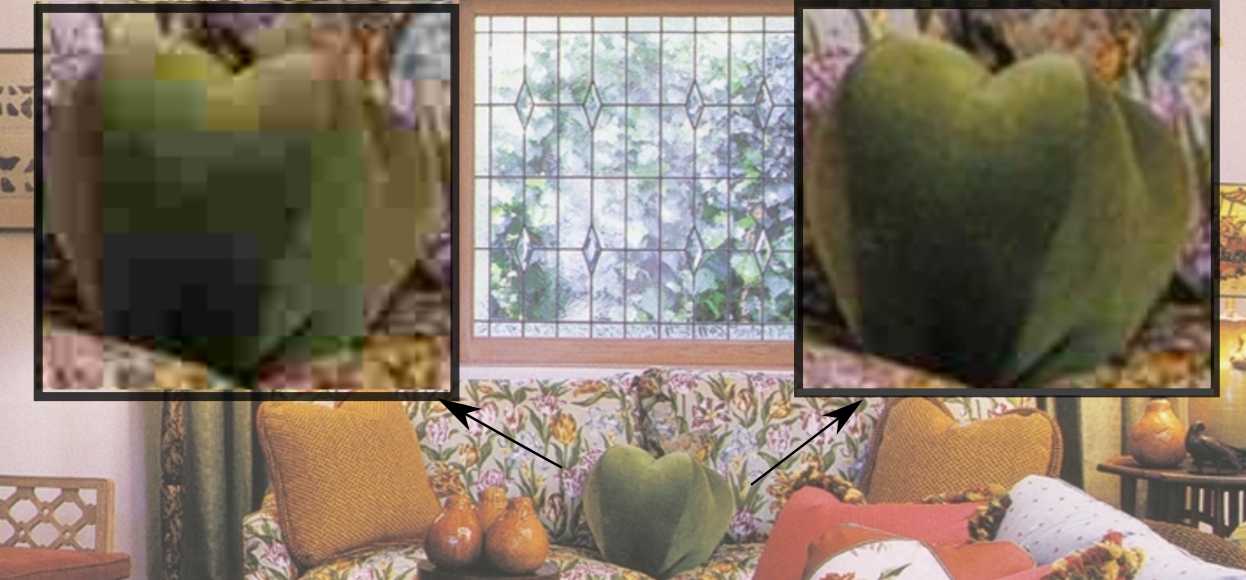
\includegraphics[scale=0.40]{figures/semantic/arrow_small.png}
    \caption[Comparison with JPEG]{Comparison of compression of semantic objects in standard \textsc{jpeg}[left] and our model [right]\label{fig_compressing_demo}}
\end{figure}

\textsc{cnn}s have been successfully applied to a variety of computer vision tasks \cite{krizhevsky2012imagenet}.
The feature extraction and transfer learning capabilities of \textsc{cnn}s are well known \cite{zeiler2014visualizing}, as are their ability to classify images by their most prominent object \cite{he2015deep}, and compute a bounding box \cite{girshick2014rich}.
Some success has been obtained in predicting the visual saliency map of a given image \cite{jiang2015salicon},\cite{kummerer2014deep}.
Previous work has shown that semantic object detection has a variety of advantages over saliency maps \cite{mnih2014recurrent}, \cite{zund2013content}.
Semantic detection recognizes discrete objects and is thus able to generate maps that are more coherent for human perception.
Visual saliency models are based on human eye fixations, and thus produce results which do not capture object boundaries \cite{kummerer2014deep}.
This is evident in the results obtained by Stella et al \cite{stella2009image}, in which image compression is guided by a multi-scale saliency map, and the obtained images show blurred edges and soft focus.

We present a \textsc{cnn} designed to locate multiple regions of interest (\textsc{roi}) within a single image.
Our model differs from traditional object detection models like \cite{dai2016r}, \cite{girshick2014rich} as these models are restricted to detecting a single salient object in an image.
It captures the structure of the depicted scene and thus maintains the integrity of semantic objects, unlike results produced using human eye fixations \cite{liu2015predicting}.
We produce a single class-invariant feature map by learning separate feature maps for each of a set of object classes and then summing over the top features.
Because this task does not require precise identification of object boundaries, our system is able to capture multiple salient regions of an image in a single pass, as opposed to standard object detection \textsc{cnn}s, which require multiple passes over the image to identify and locate multiple objects.
Model training need only be done offline, and encoding with our model employs a standard \textsc{jpeg} encoder combined with efficient computation of saliency maps (over 60 images per second for 1920x1080 using a Titan X Maxwell \textsc{gpu}).
A key advantage of our approach is that its compressed output can be decoded by any standard off-the-shelf \textsc{jpeg} implementation.  It serves to maintain the existing decoding complexity, the primary issue for distribution of electronic media.
In contrast to grid based features as described by Yuri et al \cite{reznik2013coding} our features are scale and translation invariant, which allows application of the model to a wider class of images.


% TODO fix section numbers
Section 2 reviews \textsc{cnn} techniques used for object localization, semantic segmentation and class activation maps. We also discuss merits of using our technique over these methods.
Section 3 presents our new model which can generate a map showing multiple regions of interest. In Section 4 show how we combine this map to make \textsc{jpeg} semantically aware.
Sections 5 presents experimental results on a variety of image datasets and metrics. Section 6 concludes with future areas for research.

%%%%%%%%%%%%%%%%%%%%%%%%%%%%%%%%%%%%%%%%%%%%%%%%%%%%%%%%%%%%%%%%%%%%%%%%%%%%%%%%%%%%%%%%%%%%%%%%%%%%%%%%%%%%%%%%%%%%%%%%%%%%%%%%%%%%%%

\section{Review of localization using CNNs}
%%%%%%%%%%%%%%%%%%%%%%%%%%%%%%%%%%%%%%%%%%%%%%%%%%%%%%%%%%%%%%%%%%%%%%%%%%%%%%%%%

\textsc{cnn}s are multi-layered feed-forward architectures where the learned features at each level are the weights of the convolution filters to be applied to the output of the previous level. Learning is done via gradient-based optimization \cite{lecun1995convolutional}.
\textsc{cnn}s differ from fully connected neural networks in that the dimensions of the learned convolution filters are, in general, much smaller than the dimensions of the input image, so the learned features are forced to be localized in space. Also, the convolution operation uses the same weight kernel at every image location, so feature detection is spatially invariant.


Given an image $x$, and a convolution filter of size $n \times n$, then a convolutional layer performs the operation shown in equation \ref{eqn_cnn}, where $\mathbf{W}$ is the learned filter.

\begin{equation}
    y_{ij} = \sum_{a=0}^{n} \sum_{b=0}^{n} \; \mathbf{W}_{ab} \; x_{(i+a)(j+b)}
    \label{eqn_cnn}
\end{equation}

In practice, multiple filters are learned in parallel within each layer, and thus the output of a convolution layer is a 3-\textit{d} feature map, where the depth represents the number of filters. The number of features in a given layer is a design choice, and may differ from layer to layer.
\textsc{cnn}s include a max pooling \cite{lecun1995convolutional} step after every or every other layer of convolution, in which the height and width of the feature map (filter response) are reduced by replacing several neighboring activations (coefficients), generally within a square window, with a single activation equal to the maximum within that window.  This pooling operation is strided, but the size of the pooling window can be greater than the stride, so windows can overlap.
This results in down-sampling of input data, and filters applied to such a map will have a larger receptive field (spatial support in the pixel space) for a given kernel size, thus reducing the number of parameters of the \textsc{cnn} model and allowing the training of much deeper networks.
Max pooling performed with a stride of $ k \times k $ will reduce a feature matrix of size $ N \times N $ to $ \frac{N}{k} \times \frac{N}{k}$.
This does not change the depth of the feature map, but only its width and height.
In practice, pooling windows are typically of size $2 \times 2$ or $4 \times 4$, with a stride of two, which reduces the number activations by 75\%.
\textsc{cnn}s apply some form of non-linear operation such as sigmoid $ (1-e^{-x})^{-1} $ or linear rectifier $max(0,x)$ on the output of each convolution operation.


Region-based \textsc{cnn}s use a moving window to maximize the posterior of the presence of an object \cite{girshick2015fast}.
However, this is computationally expensive as it requires looking for all possible classes in all possible regions.
Faster \textsc{rcnn}s \cite{ren2015faster} have been proposed, but they are still computationally expensive and are limited to determining the presence or absence of a single class of object within the entire image.
Moving-window methods are able to produce rectangular bounding boxes, but cannot produce object silhouettes.
In contrast, recent deep learning models proposed for semantic segmentation \cite{long2015fully}, \cite{girshick2014rich}, \cite{zheng2015conditional} are very good at drawing a close border around the objects.
However, these methods do not scale well to more than a small number of object categories (e.g. $20$) \cite{everingham2010pascal}.
Segmentation methods typically seek to produce a hard boundary for the object, in which every pixel is labeled as either part of the object or part of the background.
In contrast, class activation mapping produces a fuzzy boundary and is therefore able to capture pixels which are not part of any particular object, but are still salient to some spatial interaction between objects.
Segmentation techniques are also currently limited by the requirement for strongly-labeled data for training.
Obtaining training data where the locations of all the objects in the images are tagged is expensive and not scalable \cite{everingham2010pascal}. Our approach only requires image-level labels of object classes, without pixel-level annotation or bounding-box localization.

\subsection{Class Activation Mapping}
%%%%%%%%%%%%%%%%%%%%%%%%%%%%%%%%%%%%%%%%
Convolution filters learned from natural images are sensitive to the object classes in the training data \cite{oquab2015object}, \cite{lin2013network}.
In other words, regions of an image which contain relevant objects tend to produce high activations when convolved with learned filters, while regions that do not contain any object class have lower activations, and this is particularly true for the deeper levels of the \textsc{cnn}.
In a traditional \textsc{cnn}, there are two fully-connected (non-convolutional) layers as the final layers of the network. 
%neurons at end of the pipeline, with connections to every activation from the feature map of the previous layer.
The final layer has one neuron for every class in the training data, and the final step in the inference is to normalize the activations of the last layer to sum to one.
The second to last layer, however, is fully connected to the last convolution layer, and a non-linearity is applied to its activations.
The authors of \cite{oquab2015object}, \cite{CAMZhou2016LearningDF} modify this second to last layer to allow for class localization.
In their architecture, the second to last layer is not learned, but consists of one neuron for each feature map, which has fixed  equally-weighted connections to each activation of its corresponding map.
They suggest one neuron for each feature map from the last convolution layer, and this neuron has connections of equal weight to every activation of its feature map and no connections to any other feature map.
No non-linearity is applied to the outputs of these neurons, so that each activation in this layer represents the global spatial average of one feature map from the previous layer.
Since the output of this layer is connected directly to the classification layer, each class will in essence learn a weight for each feature map from the final convolution layer.
Thus, given an image and a class, the classification weights for that class can be used to re-weight the layers of activations of the final convolution layer on that image.
These activations can be collapsed along the feature axis to create a class activation map, spatially localizing the best evidence for that class within that image. 
Taking the spatial average of the feature map (global average pooling) at the last convolution layer reveals possible locations of objects within the image \cite{oquab2015object}, \cite{CAMZhou2016LearningDF}. 
This is used to make Class Activation Maps (CAM), which shows the probability distribution of the most likely class.

While standard max pooling combines spatially local activations for each feature independently, `global max pooling' instead combines the activations of all features for each spatial location.  
This collapses the feature map to two spatial dimensions by reducing the $D$ features at each location to a single maximum value.
If the activation of a convolution layer is of size $ M \times N \times D $ where $M$ and $N$ are the spatial dimensions of feature activations and $D$ denotes the number of features in the feature map, then after `global max pooling', the size of activations becomes $M \times N$.
It is important to note that global average pooling is performed in lieu of a final fully-connected layer (or perceptron), which is often used in image classification tasks \cite{Simonyan2014VeryDC}.
Fully-connected layers have dense connections across all neurons and thus do not preserve spatial locality of activations.
The substitution of a global max pooling layer retains this locality property in exchange for a fractional loss of classification accuracy\cite{oquab2015object}.
Pooling of feature maps is probabilistic \cite{li2015beyond}, which means the most salient object is not always the one with highest activation across the feature map. 
If we plot the activation of each feature on the $2$-dimensional map and overlay them on each other, we find significant overlap of regions of high activations.
This means taking a `global max pooling' would lead to missing some. 
Zhou \cite{CAMZhou2016LearningDF} reported that they obtained better localization by performing `global average pooling' instead of `global max pooling'. 
This is because taking an average across the feature map ensures each detected object has consistently high activations across many features, instead of a single maximal activation of one feature.
The application of GAP after the final layer of convolution $ y_{ij} $ over $\mathbf{D}$ features would result in --
CAM is obtained by taking output of the last convolution layer $f(x,y)$, and taking a weighted sum across the feature map.
Figure~\ref{fig_comparison_of_map} (c) shows an example of such a map, the equation of which is given by

\begin{equation}
    M_c(x,y) = \sum_{d \; \epsilon \; \mathbf{D}} w^{c}_{d} \; f_d(x,y)
    \label{eqn_gap}
\end{equation}

{\setlength{\parindent}{0cm} where $ w^{c}_{d} $ is the learned weight of class $c$ for feature map $d$.
%in the supervised training, and $\mathbf{D}$ the set of the numbers of filters for each layer.
M is referred to as class activation mapping (CAM) ~\ref{fig_comparison_of_map}.
 It is used to generate discriminative localization for the most probable class.
Training for \textsc{cam} minimizes the cross entropy between objects' true probability distribution over classes (all mass given to the true class) and the predicted distribution, which is obtained as }

\begin{equation}
    P(c) = \frac{\text{exp}(\sum_{xy}{M_c(x,y)})}{\sum_c \text{exp}(\sum_{xy}{M_c(x,y)})}
    \label{eqn_posterior}
\end{equation}

Since \textsc{cam}s are trained to maximize posterior probability for the class, they tend to only highlight a single most prominent object.
This makes them useful for studying the output of \textsc{cnn}s, but not well suited to more general semantic saliency, as real world images  typically contain multiple objects of interest.
This has practical applications in understanding and visualizing convolution neural networks but is less applicable to real world images, which typically contain multiple objects of interest.
Without using standard resolution, color-space or types of object classes it is hard to use such systems to extract semantic information from the images.

\section{Multi-Structure Region of Interest}
%%%%%%%%%%%%%%%%%%%%%%%%%%%%%%%%%%%%%%%%%%%%%%%%%%%%%%%%%%%%%%%%%%%%%%%%%%%%%%%%
We have developed a variant of \textsc{cam} which balances the activation for multiple objects and thus does not suffer from the issues of global average pooling.
Our method, \textit{Multi-Structure Region of Interest} (MS-ROI), allows us to effectively train on localization tasks independent of the number of classes.
For the purposes of semantic compression, obtaining a tight bound on the objects is not important. However, identifying and approximately locating all the objects is critical.
We propose a set of 3D feature maps in which each feature map is learned for an individual class, and is learned independently of the maps for other classes.
For $ \mathbf{L} $ layers, where each layer $l$ contains $d_l$ features, an image of size $ n \times n $, and with $\mathbf{C}$ classes, this results in a total activation size of

\begin{equation*}
    \sum_{l \; \epsilon \; \mathbf{L}}{d_l \times \mathbf{C} \times \frac{n}{k^l} \times \frac{n}{k^l}}
\end{equation*}

where $k$ is the max pooling stride size.
This is computationally very expensive, and not practical for real world data.
\textsc{cnn}s designed for full-scale color images have many filters per layer and are several layers deep.
For such networks, learning a model with that many parameters would be unfeasible in terms of computational requirements.
We propose two techniques to make this idea feasible for large networks: 

\begin{enumerate}[i]
	 \item Reduce the number of classes and increase the inter-class variance by combining similar classes
    \item Share feature maps across classes to jointly learn lower level features
\end{enumerate}

Most \textsc{cnn} models are built for classification on the Large Scale Visual Recognition Challenge, commonly known as ImageNet.
\footnote{http://image-net.org/challenges/LSVRC/}.
ImageNet has one thousand classes and many of the classes are fine-grained delineations of various types of animals, flowers and other objects.
We significantly reduce the number of classes by collapsing these sets of similar classes to a single, more general class.
This is desirable because, for the purpose of selecting a class invariant `region of interest,' we do not care about the differences between Siberian husky and Eskimo dog or between Lace-flower and Tuberose.
As long as objects of these combined classes have similar structure and are within the same general category, the map produced will be almost identical.
Details of the combined classes used in our model are provided in the Experimental Results section.

It is self-evident that most images contain only a few classes and thus it is computationally inefficient to build a separate feature map for every class.
More importantly, many classes have similar lower-level features, even when the number of classes is relatively small.
The first few layers of a \textsc{cnn} learn filters which recognize small edges and motifs \cite{zeiler2014visualizing}, which are found across a wide variety of object classes.
Therefore, we propose parameter sharing across the feature maps for different classes.
This reduces the number of parameters and also allows for the joint learning of these shared, low-level features.

\begin{figure}[H]
    \centering
    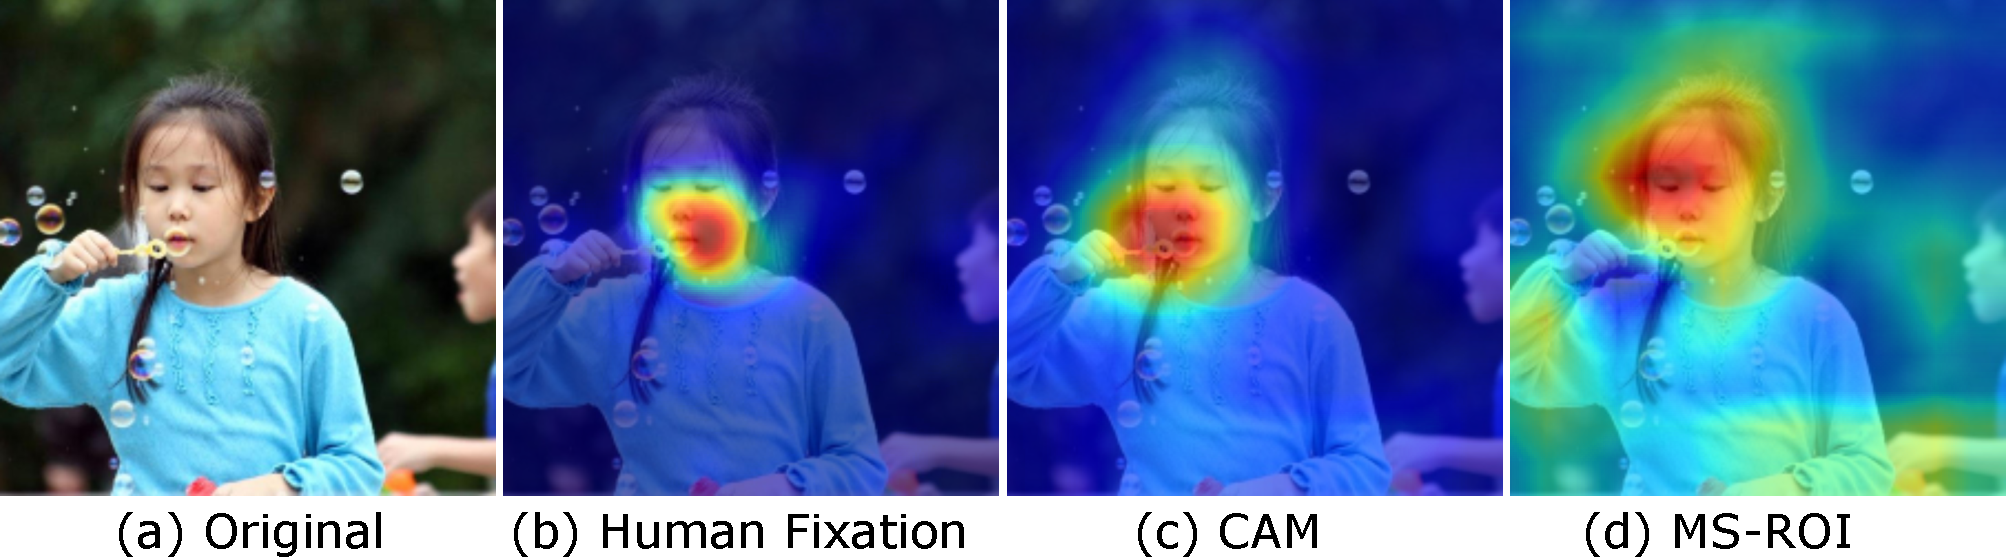
\includegraphics[scale=0.49]{figures/semantic/girl_compression.pdf}
    \caption[MSROI vs CAM vs Saliency]{Comparison of various methods of detecting objects in an image \label{fig_comparison_of_map}}
\end{figure}

Although we do not restrict ourselves to a single most-probable class, it is desirable to eliminate the effects of activations for classes which are not present in the image.  
In order to accomplish this, we propose a thresholding operation which discards those classes whose learned features do not have a sufficiently large total activation when summed across all features and across the entire image.  
Let $Z^c_l$ denote the total sum of the activations of layer $\ell$ for all feature maps for a given class $c$.
Since our feature map is a $4$-dimensional tensor, $Z^c_l$ can be obtained by summation of this tensor over the three non-class dimensions.

\begin{equation}
    Z^c_l = \sum_{d \; \epsilon \; \mathbf{D}} \sum_{x,y} f_d^c(x,y)
    \label{eqn_Zscore}
\end{equation}

Next, we use $Z^c_l$ to filter the classes. Computation of the multi-structure region of interest is shown below.

\begin{equation}
    \hat{M}(x,y) = \sum_{c \; \epsilon \; \mathbf{c} }
    \begin{cases}
        \sum_d f_d^c(x,y), & \text{if}\ Z^c_l > T \\
        \phantom{this_is_empty} \\
      0 & \text{otherwise}
    \end{cases}
    \label{eqn_msroi}
\end{equation}

We use the symbol $\hat{M}$ to denote the multi-structure map generated by our proposed model in order to contrast it with the map generated using standard \textsc{cam} models, $ M $.
$ \hat{M} $ is a sum over all classes with total activations $Z^c_l$ beyond a threshold value $T$.
$T$ is determined during the training or chosen as a hyper-parameter for learning. 
In practice, it is sufficient to \textit{argsort} $Z^c_l$ and pick the top five classes and combine them via a sum weighted by their rank. 
It should be noted that, because $ \hat{M} $ is no longer a reflection of the class of the image, we use the term `region of interest'.

A comparison of our model (MS-ROI) with \textsc{cam} and human fixation is shown in Figure~\ref{fig_comparison_of_map}. 
Only our model identifies the face of the boy on the right as well the hands of both children at the bottom. 
When doing compression, it is important that we do not lower the quality of body extremities or other objects which other models may not identify as critical to the primary object class of the image.
If a human annotator were to paint the areas which should be compressed at better quality, we believe the annotated area would be closer to that captured by our model.

To train the model to maximize the detection of all objects, instead of using a softmax function as in equation \ref{eqn_posterior}, we use sigmoid, which does not marginalize the posterior over the classes.
Thus the likelihood of a class $c$ is given by equation~\ref{eqn_our_posterior}. 

\begin{equation}
    P(c) = \frac{1}{1 + \text{exp}(Z^c_l)}
    \label{eqn_our_posterior}
\end{equation}

\section{Integrating MS-ROI map with JPEG}
%%%%%%%%%%%%%%%%%%%%%%%%%%%%%%%%%%%%%%%%%%%%%%%%%%%%%%%%%%%%%%%%%%%%%%%%%%%%%%%%
We obtain from MS-ROI a saliency value for each pixel in the range [0,1], where 1 indicates maximum saliency.
Then discretize these saliency values into $k$ levels, where $k$ is a tune-able hyper-parameter.
The lowest level contains pixels of saliency $[0,1/k]$, the second level contains pixels of saliency $(1/k,2/k]$ and so forth.
We next select a range of \textsc{jpeg} quality levels, $Q_l$ to $Q_h$.  Each saliency level will be compressed using a $Q$ value drawn from this range, corresponding to that level.
In other words, saliency level $n$, with saliency range $[n/k,(n+1)/k]$ will be compressed using 

\begin{equation}
Q_n = Q_l + \frac{n*(Q_h - Q_l)}{k}
\end{equation}


For each level $l \le n \le h$, we obtain a decoded \textsc{jpeg} of the image after encoding at quality level $Q_n$.
For each $8 \times 8$ block of our output image, we select the block of color values obtained by the \textsc{jpeg} corresponding to that block's saliency level.  This mosiac of blocks is finally compressed using a standard \textsc{jpeg} encoder with the desired output quality to produce a file which can be decoded by any off-the-shelf \textsc{jpeg} decoder.

Details of our choices for $k$, $Q_l$ and $Q_h$, as well as target image sizes are provided in the next section.  A wider range of $Q_l$ and $Q_h$ will tend to produce stronger results, but at the expense of very poor quality in non-salient regions.

\begin{algorithm}[H]
\SetKwInOut{Input}{Input}
\SetKwInOut{Output}{Output}

    \Input{Image: I}
    \Output{Image: O, same dimensions as I}
    Let $Q_{l \cdot h}$ be N fixed values in range l to h
    
    \For{b $\gets 8 \times 8$ blocks in I}{
        $Q_i = \hat{M}$[b] \#Nearest\ quantized\ level
        
        I'[b] $\gets$ JPEG \{I[b], $Q_i$\}
    }
    O $\gets$ JPEG\{I', $Q_f$\}
\caption[Encoding with MSROI]{JPEG Encoding with MSROI}
\label{alg:encoding}
\end{algorithm}

Encoding of image using MSROI on a JPEG standard can be summarized as shown by algorithm ~\ref{alg:encoding}.

Figure ~\ref{fig_encoding_steps} shows the steps of taking an image and using the MSROI map to obtain the final encoded image.

\begin{figure}[H]
    \centering
    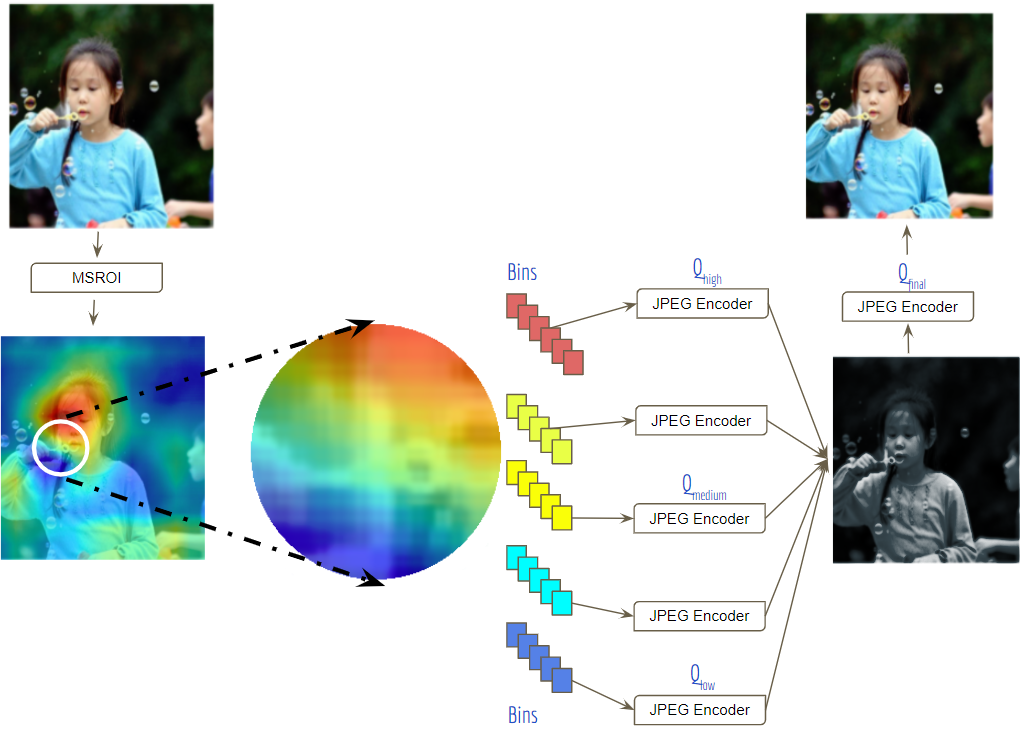
\includegraphics[scale=0.65]{figures/semantic/variable_q_jpeg.png}
    \caption[Encoding with MSROI]{Process of combining MSROI maps to obtain final encoded image \label{fig_encoding_steps}}
\end{figure}


\section{Experimental Results}
%%%%%%%%%%%%%%%%%%%%%%%%%%%%%%%%%%%%%%%%%%%%%%%%%%%%%%%%%%%%%%%%%%%%%%%%%%%%%%%%%
We trained our model with the Caltech-256 dataset \cite{griffin2007caltech}, which contains 256 classes of man-made and natural objects, common plants and animals, buildings, etc.

We believe this offers a good balance between covering more classes as compared to CIFAR-100 which contains only 100 classes, and avoiding overly finely-grained classes as in ImageNet with 1000 classes \cite{imagenet_cvpr09}.
For the results reported here, we experimented with several stacked layers of convolution as shown in the diagram below:
\begin{equation*}
    \text{IMAGE} \longmapsto \bigg[ \big[ \text{CONV} \rightarrow \text{RELU}\big]^2 \rightarrow \text{MAXPOOL} \bigg]^5 \longmapsto \text{MS-ROI} \longmapsto \text{MAP}
\end{equation*}


$\text{MS-ROI}$ refers to the operation shown in the equation~\ref{eqn_msroi}.
To obtain the final image we discretize the heat-map into five levels and use \textsc{jpeg} quality levels $Q$ in increments of ten from $Q_l=30$ to $Q_h=70$.
For all experiments, the file size of the standard \textsc{jpeg} image and the \textsc{jpeg} obtained from our model were kept within $\pm1\%$ of each other.
On average, salient regions were compressed at $Q_f=65$, and non-salient regions were compressed at $Q=45$.
The average $Q$ for the final image generated using our model was $55$, whereas for all standard \textsc{jpeg} samples, $Q$ was chosen to be 50. It should be noted that even though images are at different $Q$ they have same size.

\begin{figure}[H]
    \centering
    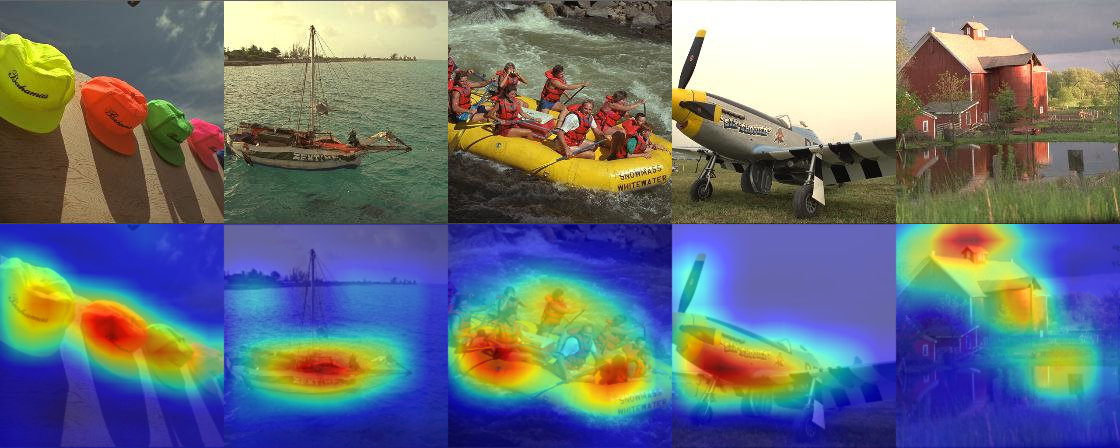
\includegraphics[scale=0.43]{figures/semantic/all_images_small.png}
    \caption[Results on KODAK]{Sample of our map for five KODAK images.\label{fig_kodak_combo}}
\end{figure}

We tested on the Kodak PhotoCD set (24 images) and the the MIT dataset (2,000 images).
Kodak is a well known dataset consisting primarily of natural outdoor color images.
Figure~\ref{fig_kodak_combo} shows a sample of five of these images, along with the corresponding heatmaps generated by our algorithm; the first four show typical results which strongly capture the salient content of the images, while the fifth is a rare case of partial failure, in which the heatmap does not fully capture all salient regions.
The MIT set allows us to compare results across twenty categories. In Table~\ref{tbl_results} we only report averaged results across `Outdoor Man-made' and `Outdoor Natural' categories (200 images), as these categories are likely to contain multiple semantic objects, and are therefore appropriate for our method.
Both datasets contain images of smaller resolutions, but the effectiveness of perceptual compression is more pronounced for larger images.
Therefore, we additionally selected a very large image of resolution $8705\times8400$, which we scale to a range of sizes to demonstrate the effectiveness of our system at a variety of resolutions.
See Figure~\ref{fig_size} for the image sizes used in this experiment.
Both Figure~\ref{fig_size} and Figure~\ref{fig_mit} show the \texttt{PSNR-HVS} difference between our model and standard \textsc{jpeg}. Positive values indicate our model has higher performance compared to standard \textsc{jpeg}.
In addition to an array of standard quality metrics, we also report a \texttt{PSNR} value calculated only for those regions our method has identified as salient, which we term \texttt{PSNR-S}.
By examining only regions of high semantic saliency, this metric demonstrates that our compression method is indeed able to preserve visual quality in targeted regions, without sacrificing performance on traditional image-level quality metrics or compression ratio.
It should be noted that the validity of this metric is dependent on the correctness of the underlying saliency map, and thus should only be interpreted to demonstrate the success of the final image construction in preserving details highlighted by that map.

\begin{table}[H]
% \footnotesize
\centering
\rowcolors{1}{White}{Gray}
\begin{tabular}{lccccccc}
			 \toprule
               & \texttt{PSNR-S} \phantom{so} & \texttt{PSNR} \phantom{so} & \texttt{PSNR-HVS} \phantom{so}& \texttt{PSNR-HVSM} \phantom{so}& \texttt{SSIM} \phantom{so}& \texttt{MS-SSIM} \phantom{so}& \texttt{VIFP}\phantom{so} \\
              \midrule
              & \multicolumn{6}{c}{Kodak PhotoCD [24 images]}   &                        \\
              \midrule
Std \textsc{jpeg} &   33.91   & 34.70     & 34.92          & 42.19  & 0.969  & 0.991 & 0.626      \\
% 			  \midrule
			  \cline{2-8}
Our model &  39.16    & 34.82    & 35.05          & 42.33  & 0.969  & 0.991 & 0.629     \\
			  \midrule
              & \multicolumn{6}{c}{MIT Saliency Benchmark [Outdoor Man-made + Natural, 200 images]} &              \\
			  \midrule
Std \textsc{jpeg} & 36.9 & 31.84    & 35.91   & 45.37 & 0.893 & 0.982     & 0.521      \\
% 			  \midrule
			  \cline{2-8}
Our model & 40.8 & 32.16   & 36.32   & 45.62 &  0.917 & 0.990      & 0.529      \\
			  \midrule
              & \multicolumn{6}{c}{Re-sized images of a very large image, see fig:~\ref{fig_size} [20 images]} &          \\
			  \midrule
Std \textsc{jpeg} & 35.4   & 27.46  & 33.12 & 43.26     & 0.912 & 0.988 & 0.494     \\
% 			  \midrule
			  \cline{2-8}
Our model & 39.6  & 28.67  & 34.63 & 44.89     & 0.915 & 0.991 & 0.522     \\
			  \toprule
\end{tabular}
\caption[Results across various datasets]{Results across datasets \label{tbl_results}}
\end{table}
        
\begin{figure}[H]
    \centering
    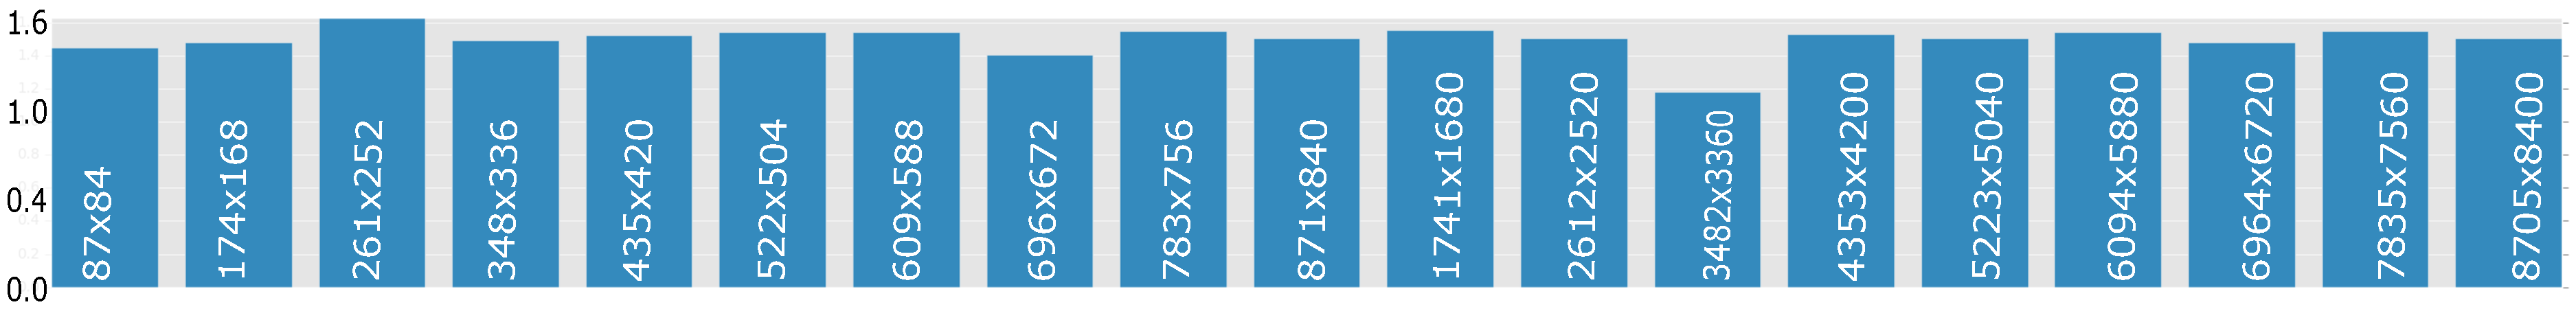
\includegraphics[scale=0.28]{figures/semantic/image_size.pdf}
    \caption[Impact on Image Size]{\texttt{PSNR-HVS} of our model - \textsc{jpeg} across various image size (higher is better). \label{fig_size}}
\end{figure}

\begin{figure}[H]
    \centering
    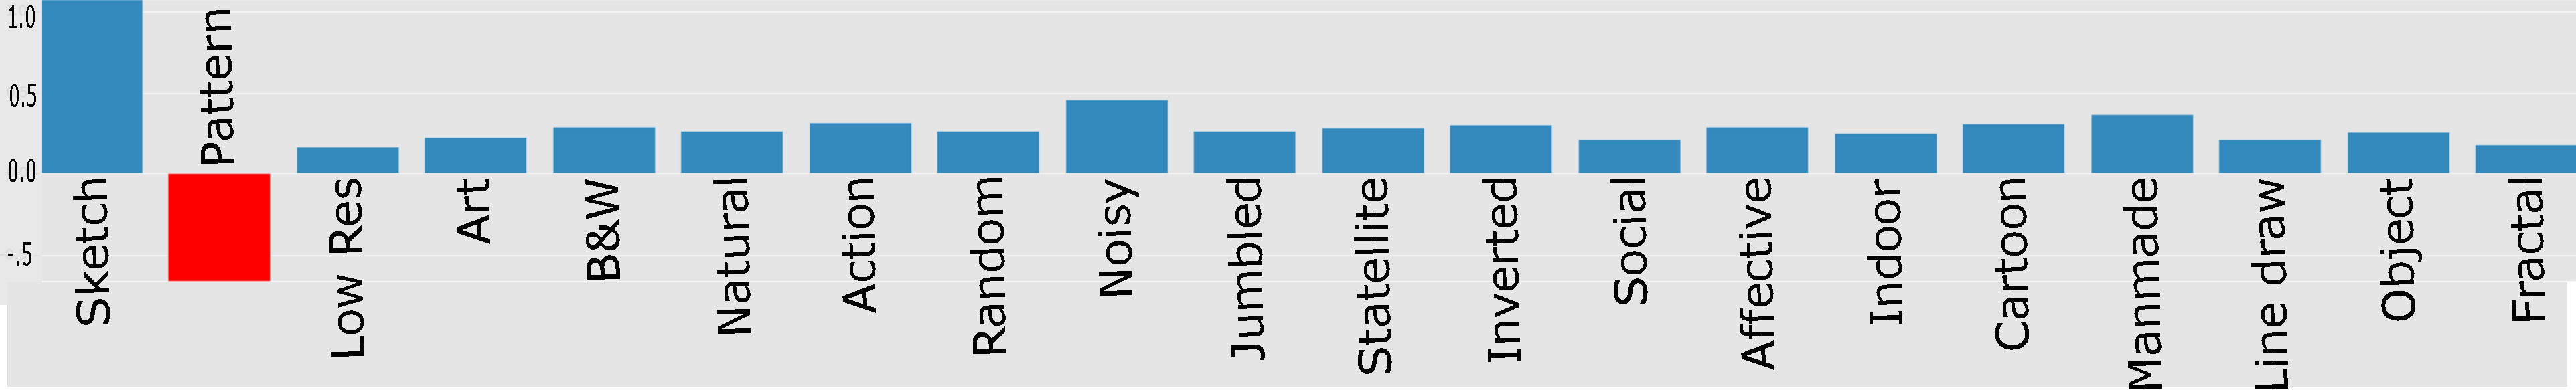
\includegraphics[scale=0.28]{figures/semantic/image_mit.pdf}
    \caption[Impact on Image Type]{\texttt{PSNR-HVS} of our model - \textsc{jpeg} across various categories of MIT Saliency dataset (higher is better). \label{fig_mit}}
\end{figure}

\section{Discussion}
%%%%%%%%%%%%%%%%%%%%%%%%%%%%%%%%%%%%%%%%%%%%%%%%%%%%%%%%%%%%%%%%%%%%%%%%%%%%%%%%
While the comparison of metrics in Table~\ref{tbl_results} on standard \textsc{jpeg} and variable quality \textsc{jpeg} using our  generated map is similar, it should be noted that these metrics still lack ability to judge human perception. 
It is evident from the results that the salient objects have significantly higher \texttt{PSNR-S}, yet maintains overall \texttt{PSNR} and the file size.
We believe we have effectively created a model to make \textsc{jpeg} semantically aware without sacrificing overall image quality.
We know from the \textsc{jpeg} standard that images compressed with higher $Q$ better, and by design our model compresses the salient objects with higher $Q$; see Figure~\ref{fig_compressing_demo} for qualitative evaluation.

The results in Table~\ref{tbl_results} show the success of our method in maintaining or improving performance on traditional image quality metrics.
Further, given the efficacy of our method in identifying multiple regions of interest, the \texttt{PSNR-S} measurements demonstrate the power of our method to produce superior visual quality in subjectively important regions.

When we look at Figure~\ref{fig_compressing_demo} we see the difference in quality of the salient object.  
Our model consistently outperforms standard \textsc{jpeg} on \texttt{SSIM} and \texttt{MS-SSIM} metric.
These metrics measure the inherent structures in the image and Richter et al \cite{richter2009ms} \cite{richter2011ssim} has shown efficacy of these metric for image compression.

Figure~\ref{fig_mit} shows the performance of our model across all categories of the MIT dataset.
Performance was strongest in categories like `Outdoor Natural', `Outdoor Man Made', `Action' and `Object', while categories like `Line Drawing', `Fractal' and `Low Resolution' showed the least improvement.
Not surprisingly, the category `Pattern', which lacks semantic objects, is the only category where our model did not improve upon standard \textsc{jpeg}.
Figure~\ref{fig_size} shows results on the same image scaled to different sizes. 
Because our model benefits from the scale-invariance of \textsc{cnn}s, we are able to preserve performance across a wide range of input sizes.
Performance of our model on \texttt{PSNR-HVS} is consistent across all tested sizes. \textsc{cnn}s are able to learn scale-invariant features, and therefore the same object at any size should always be classified similarly.
Our model preserves this feature even when looking for multiple objects.


    

\section{Conclusion}
We have presented a model which can learn to detect multiple objects at any scale and generate a map of multiple semantically salient image regions.
This provides sufficient information to perform variable-quality image compression, without providing a precise semantic segmentation.
Unlike region-based models, our model does not have to iterate over many windows.
We sacrifice exact localization for the ability to detect multiple salient objects.
Using the output of our model as a map to perform variable-quality compression preserves the overall quality and size of the image, yet improves the visual quality of salient objects.
Our variable compression improves upon visual quality without sacrificing compression ratio. 
Encoding requires a single inference over the pre-trained model, the cost of which is reasonable when performed using a \textsc{gpu}, along with a standard \textsc{jpeg} encoder. The cost of decoding, which employs a standard, off-the-shelf \textsc{jpeg} decoder remains unchanged.
We believe it will be possible to incorporate our approach into other lossy compression methods such as \textsc{jpeg} 2000 and vector quantization, a subject of future work.
Improvements to the power of our underlying \textsc{cnn}, addressing evolving visual quality metrics, and other applications such as video compression, are also potential areas of future work.


\chapter{Robust regions of interest}
\section{Introduction}
Deep neural networks (DNNs) have shown tremendous success in image recognition tasks, even surpassing human capability ~\cite{He2016DeepRL}. 
DNNs have become components of many critical systems, such as self-driving cars ~\cite{bojarski2016end}, medical image segmentation, surveillance, and  malware classification ~\cite{pascanu2015malware}. However, recent research has shown that DNNs are vulnerable to adversarial attacks, in which minute, carefully-chosen image perturbations can result in misclassification of the image by the neural network ~\cite{Goodfellow2014ExplainingAH}.
In most cases, this change is imperceptible to humans (the resulting image is visually indistinguishable from the original).

%Recently, research has shown that these adversarial attacks are very hard to detect and difficult to protect against.
%Defense is particularly challenging because the adversarial examples are transferable from one model to another, i.e an image tailored to fool one deep learning model is also likely able to fool other deep learning models.
% NEW %

Current adversarial attacks take advantage of the \emph{over-completeness} of the pixel representation of images -- that is, storing images as an array of values results in storing much more information than is required to recognize the content of an image. Traditional image compression techniques, like JPEG, rely on assumptions about the human perception of natural images in order to compress them. Since adversarial attacks are imperceptible to the human eye, they can be viewed as hiding themselves in the over-complete part of the pixel representation of images. Removing these adversarial perturbations is therefore a lossy image compression problem: by effectively encoding natural images, image compression techniques can quantize away imperceptible elements of an image, effectively blocking attacks that rely on adversarial perturbations.

%Research in defending against such adversarial perturbations is in its infancy. However, recent work ~\cite{Das2017KeepingTB,Dziugaite2016ASO} has shown that JPEG compression removes some of these imperceptible  perturbations, often times restoring the original classification of the image. 
%More advanced attacks, however, are robust against JPEG compression.

While the research in defending against such adversarial perturbations is still in its infancy, it has been shown that JPEG naturally removes some of these imperceptible  perturbations, thereby restoring the original classification of the image ~\cite{Das2017KeepingTB,Dziugaite2016ASO}.
More advanced attacks, however, are robust against JPEG compression.
In this work, we study the nature of the perturbations generated by adversarial methods, as well as their effect on classification. We present a solution which produces a standard JPEG-decodable image, while allowing significantly improved classification recovery as compared to off-the-shelf JPEG compression.
% NEW %


%Most of these attacks attempt to change the output of the model directly, using the gradient of the input image with respect to the the model output to iteratively discover a smallest perturbation to the input image that will change the model's classification. 
%NEW


Several techniques have been proposed which attempt to reduce the feasibility of generating adversarial images ~\cite{Papernot2016DistillationAA,Miyato2015DistributionalSW}. Most of these methods involve augmenting the DNN training process to create a more robust classifier.
However, these defenses often fail against more advanced attacks, and come at the cost of more computationally expensive training. 
%TODO : \ref{defenses} isn't working
%A detailed discussion of proposed defenses is found in section ~\ref{defenses}.
%If a new attack vector is proposed which falls outside of what defense was trained for, the model has to be trained with the new set of perturbations to make it robust against this new attack. 
%This is an expensive and non-scalable solution.
%In many cases, it is prohibitively expensive to retrain a classifier to defend against a new attack.

\begin{figure}[H]
     \centering
     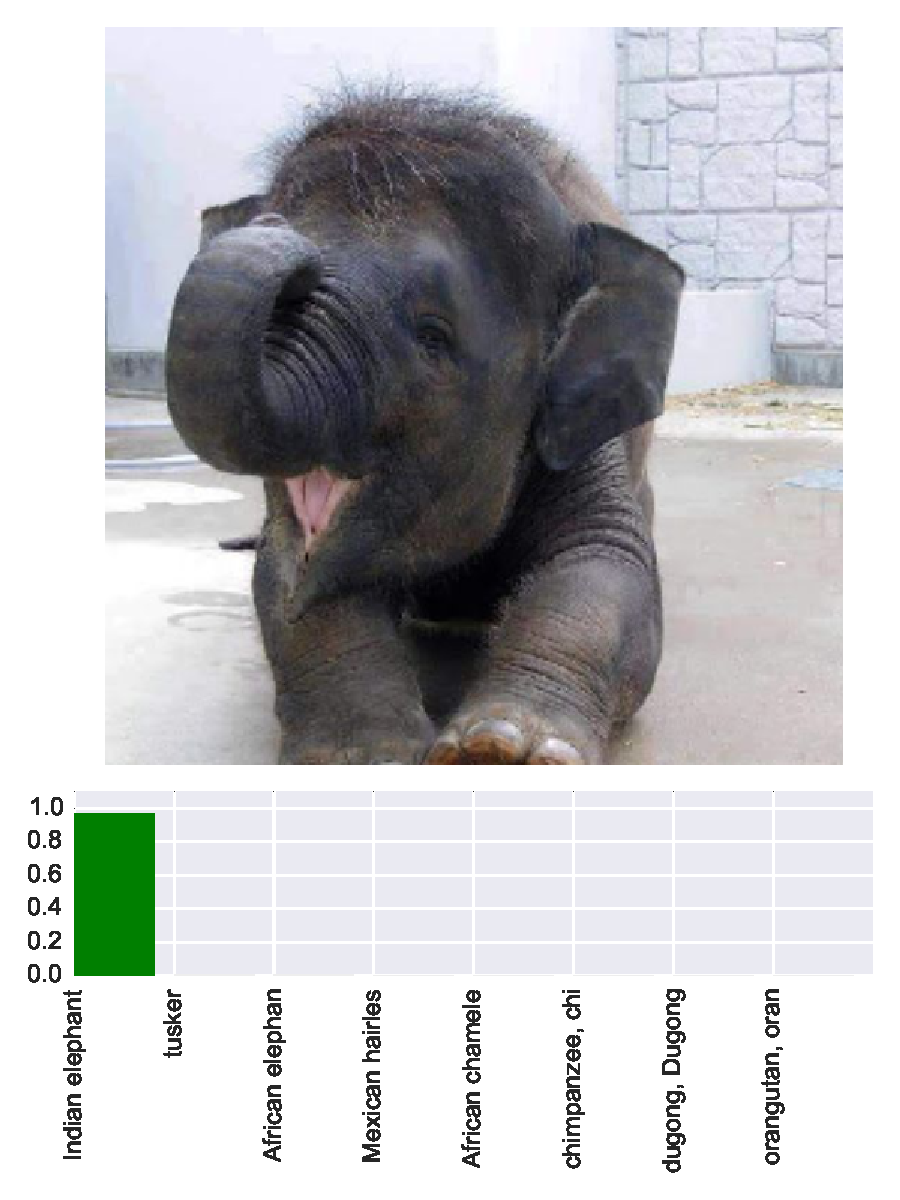
\includegraphics[width=0.30\textwidth,angle=0]{figures/protect/ori.pdf}
     
\includegraphics[width=0.04\textwidth,angle=0,scale=0.9]{figures/protect/plus_epsilon.png}
     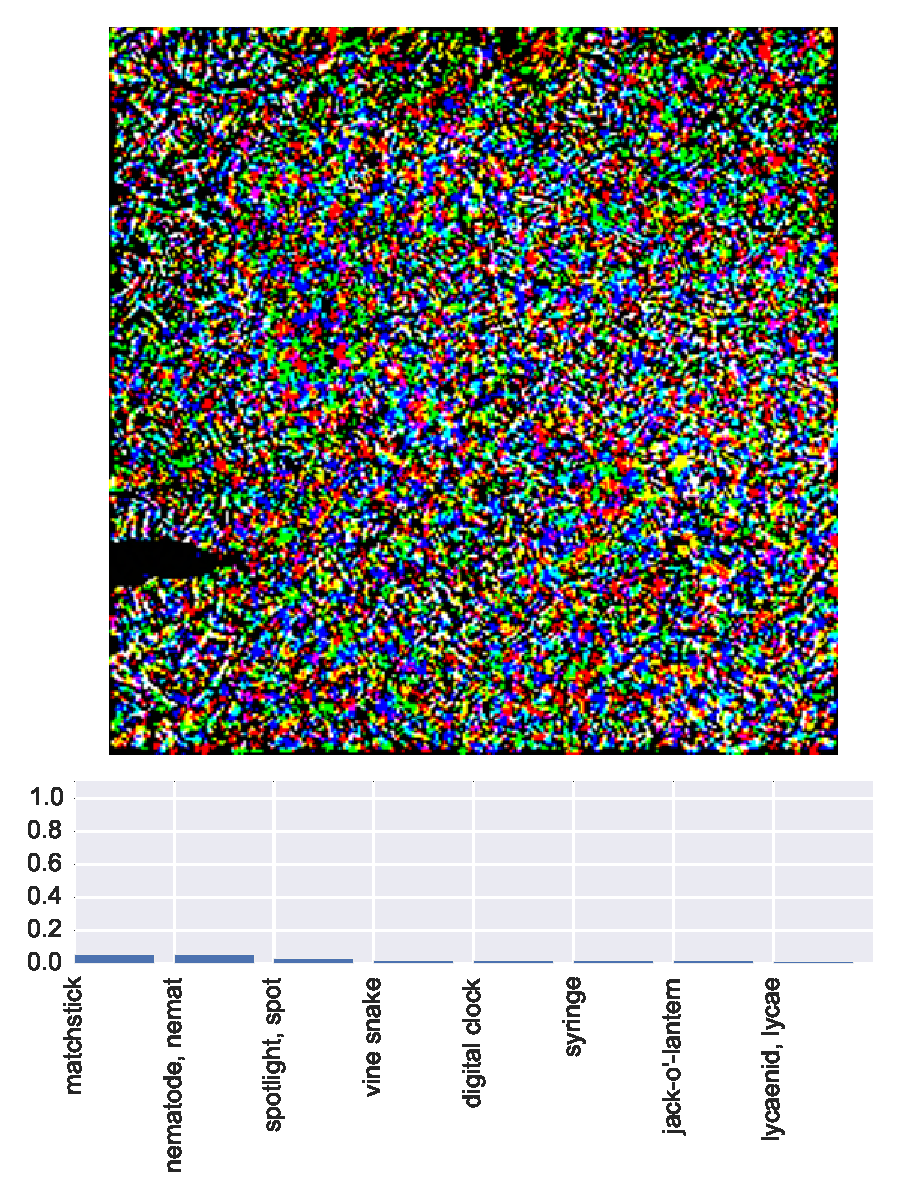
\includegraphics[width=0.30\textwidth,angle=0]{figures/protect/noise.pdf}
     
\includegraphics[width=0.03\textwidth,angle=0,scale=0.9]{figures/protect/equals.png}
     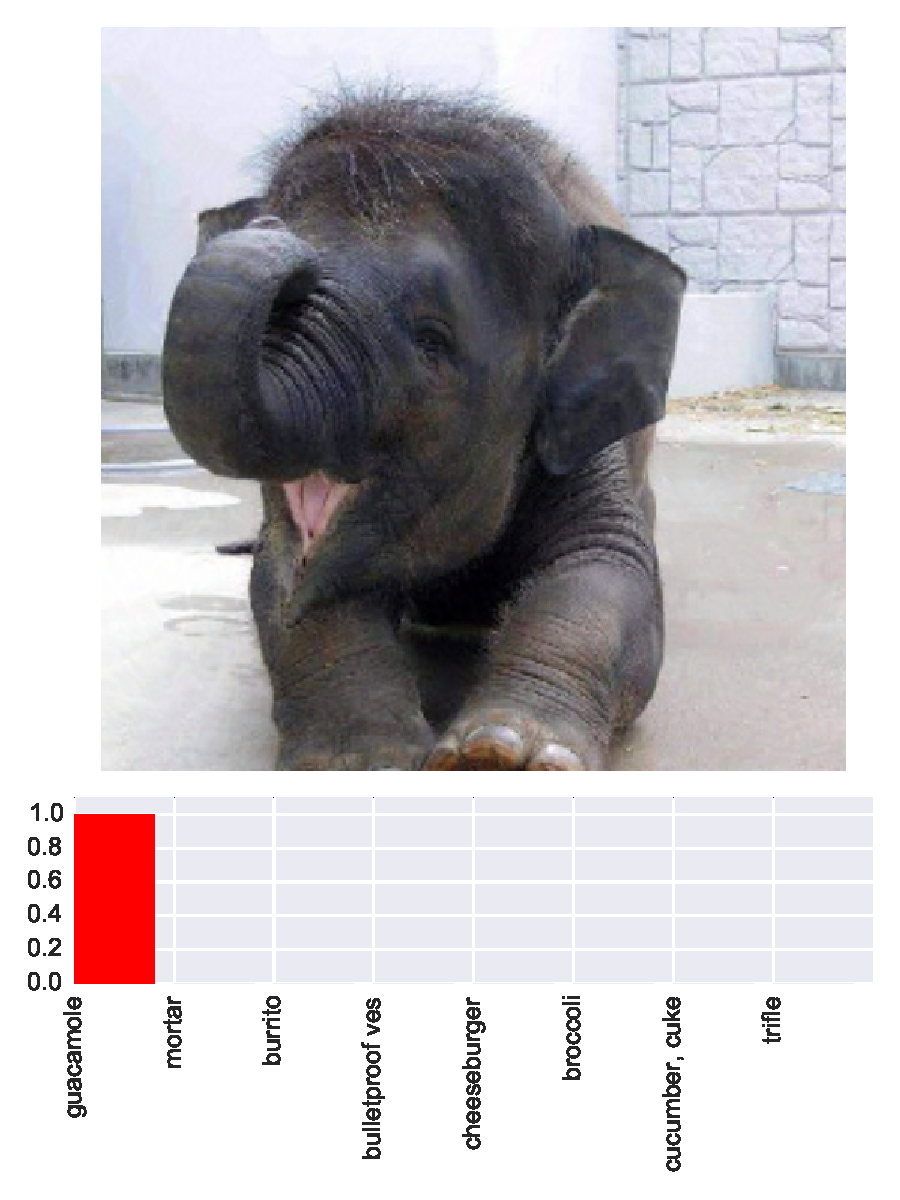
\includegraphics[width=0.30\textwidth,angle=0]{figures/protect/adv.pdf}
     \label{fig:adv}
      \caption[Qualitative comparison of Adversarial Images]{Left: Original Image, Center: Perturbed Noise, Right: Adversarial Image}
 \end{figure}

%[TODO: add +epsilon/= to figure 1]

%We therefore seek a defense which can be applied to images as a preprocessing step, before they are passed to the classifier.
%NEW an improved JPEG compressor
%We present an improved JPEG compressor which defends against such attacks without requiring changes to the classification model or its training process.
%Our algorithm dampens the noise added by the adversary so as to allow the classifier to recover the correct classification.
%While this kind of defense may not be the most robust solution, it comes at a low computational cost, and the ubiquity of the JPEG decoder makes it easily implementable in practice.
%It has a low computational cost, and decoding can still be done by any standard, off-the-shelf decoder.
%the ubiquity of the JPEG decoder makes it easily implementable in practice.

%NEW


Standard JPEG compression is able to provide some measure of defense against adversarial attacks.
Since adversarial perturbations are often high frequency and low magnitude, the quantization step of JPEG frequently removes them.
When the noise added by the adversary is removed or substantially modified, and the resulting image no longer fools the classifier.
However, as the severity of quantization increases, important features of the original image are also lost, and the model's ability to correctly classify the resulting image deteriorates regardless of any adversarial perturbation.
This trade-off limits the effectiveness of a simple JPEG-based defense, as defending against more sophisticated attacks requires harsh quantization that renders the output image difficult to classify.

Our algorithm employs an adaptive quantization scheme which intelligently quantizes different blocks at different levels. 
%Our analysis of adversarial images generated by various attacks shows that attack methods will tend to perturb all regions of an image with equal probability. %[TODO DONE: Make sure to include said analysis showing where perturbations are generated]
We have found that the regions chosen for perturations by attack methods do not strongly correlate with the presence of a semantic object.
As a result, there often exists added noise outside the object of interest in the image. We target this portion of the noise for aggressive quantization.
We tested the MSROI algorithm of  ~\cite{Prakash2017SemanticPI}, which identifies multiple salient regions of the image, and quantizes those regions which are not salient more aggressively. %[TODO: add JPEG reference]
MSROI adaptive quantization dampens a significant portion of the adversarial noise, but does so without deteriorating the quality of salient regions, thereby disrupting the attack while allowing for recovery of the original classification.
However, initial experiments demonstrated that the unmodified MSROI algorithm is also susceptible to adversarial noise, weakening the accuracy of the generated saliency maps.
%OLD
%Therefore, we strongly quantize those areas which are not identified as containing a salient object.
%This gets rid of a sufficient portion of the adversarial noise to defend against the attack, without deteriorating salient regions, thereby allowing recovery of the original classification.
%We experimented with a heat map that is trained to highlight all the salient regions of a given image  ~\cite{Prakash2017SemanticPI}. 
%We show that the accuracy of this map is also impacted by adversarial noise. 
%END OLD
Therefore, we present a more robust method of generating a saliency map, which is able to recover object saliency even in the presence of adversarial noise, without significantly impacting performance on unperturbed images.
We show that our proposed defense is successful against several state-of-the-art attack methods using an off-the-shelf classification model.
We further demonstrate that our proposed technique greatly improves upon the defense provided by a standard JPEG encoder.
%[TODODONE (removed: do JPEG2000 experiments to verify]

\section{Background}
%[TODO: add default ref for deep neural nets]
A deep neural network can be viewed as a parameterized function, $F_\theta$, which maps $x \in \mathbb{R}^n$ to $y \in \mathbb{R}^m$  i.e.\ $F_\theta(x) = y$ where $\theta$ represents the model parameters. 
Feed-forward neural networks are composed of multiple layers of successive operations, each applied to the output of the previous layer. For a deep neural network containing $l$ layers, the final network is a function composition of $l$ simpler functions i.e $F = F_1 \circ F_2 \circ \cdots F_l$.
These networks are trained by minimizing some loss function, $\mathcal{L}$, which is a differentiable measure of the classification accuracy on the training data.
%computed over the classification probabilities predicted by the network and the ground truth.
The parameters of the model, $\theta$, are learned by stochastic gradient descent (SGD). 
%[TODO: the SGD equations seem unnecessary - probably cut them to save space.  Maybe cite SGD instead?]
Let $\widetilde{y}$ denote $F(x|\theta)$.
\[
   \min \mathcal{L}(y, \widetilde{y}) = - \frac{1}{N} \sum_{i=1}^N y^i \times \log %(\widetilde{y}) + (1-y^i) \times \log(1-\widetilde{y})
\]
\[
   \theta^l := \theta^l - \eta \nabla \mathcal{L}(y,\widetilde{y})
\]

Most adversarial attack methods use the gradient of the image pixels with respect to the the classification error to generate the desired perturbation.
In order to compute this gradient, an attacker needs to have access to the internal model and parameters.
These kinds of attacks are called white box attacks, as the adversary needs access to the targeted model. 
White box attacks can fool many state-of-the-art convolutional neural networks. 
Many popular deep learning models are publicly available, making them vulnerable in practice to these attacks.
%This increases their ability to be attacked using such techniques.

%These attacks are discussed in detail in section  ~\ref{attacks}.

It is also possible to attack deep networks without access to the model parameters. 
Such attacks are called black box attacks, and they begin by training a secondary model to match the outputs of the target model.
This secondary model can then be attacked using white box methods, and the resulting adversarial images are transferable to the target network \cite{Papernot2016PracticalBA}. 
Black box attacks are weaker than white box attacks; here we focus on white box attacks. 

\section{Adversarial Attacks} \label{attacks}
Formally, the paradigm of adversarial attacks can be described as follows. 
Let $x$ be an input image to a classifier. 
Then, the class label (the model's evaluation of what object the image contains) for the image $x$ is: $c = \argmax_{i} F(x|\theta)$ where $i$ is an index into the output vector.

An adversarial attacker takes the image $x$ and adds a small perturbation $\delta_x$, to obtain an adversarial image $x' = x + \delta_x$.
The attack is considered to be successful if, for a small $\delta_x$, the class label of the adversarial image ($c'$), is not the same as that of original image ($c$). 
There is no consensus on the exact definition of  ``small'' for $\delta_x$, but attacks are generally considered successful when the difference between $x$ and $x'$ is indistinguishable to the human eye. Some attacks are noticeable to humans, but do not change our perception of the class label of the image, and these attacks are also considered successful.  %[TODO: clarify this]
Attacks can be targeted to induce a specific chosen class label, $\hat{c}$ such that $c' = \hat{c}$, or untargeted, meaning that they seek to induce any class label, as long as it does not match the original classification, i.e., $c' \neq c$.

In most cases, untargeted attacks are performed by iterating a targeted attack over all classes and choosing the class which requires the smallest perturbation.
%Targeted attacks tend to require a larger, more obvious perturbation, thereby making them easier to detect and defend against.
As our work focuses on defense, we will consider untargeted attacks, and therefore our methods should also be effective against targeted attacks.

%TODO: rephrase
Adversarial attacks work by exploiting the design of the model and the limitations of SGD. 
Just as gradients of the model parameters ($\theta$) with respect to the loss function are calculated during SGD training, an attacker can compute gradients of the input pixels with respect to the classification output.
These gradients instruct the attacker on how to modify the image to change the model's classification.
In the following sections, we will briefly describe each of the adversarial attacks used in our experiments.

%\subsection{Fast Gradient Sign Method}
\subsection{Fast Gradient Sign Method (FGSM)} 
\cite{Goodfellow2014ExplainingAH} uses the sign of the gradient of the loss function to determine the direction of the perturbation $\delta_x$. 
\[
    x' = x + \epsilon \times \text{sign}(\nabla \mathcal{L} (F(x|\theta),\widetilde{y}))
\]

Where $\epsilon$ is a small value which controls the magnitude of perturbation, chosen through trial and error.
To ensure a sufficiently small $\delta_x$, FGSM optimizes the $L_\infty$ distance between $x$ and $x'$, and thus tries to minimize the maximum change to any of the pixels.
It has been shown that with small values of $\epsilon$, most deep neural networks trained on CIFAR-10 and MNIST can easily be fooled \cite{Goodfellow2014ExplainingAH}.
FGSM is a particularly efficient attack method, as it requires only a single computation of the gradients of the input pixels.
However, FGSM does not always produce robust results.%, and may not be successful against all classes. 
%[TODO: what does "against all classes" mean?]

\subsection{Iterative Gradient Sign Method}
\cite{Kurakin2016AdversarialEI} builds upon FGSM.
Starting with the original image, FGSM is applied iteratively until a satisfactory image is found, and, at each step, the generated adversarial image is clipped so that the generated image is within an $L_\infty$ $\epsilon$-neighborhood of the original image.
\[
x_0' = x, \qquad x_{N+1}' = \text{Clip}_{x,\epsilon} \Bigl\{x_N' + \alpha \times \text{sign}(\nabla \mathcal{L} (F(x|\theta),\widetilde{y}))  \Bigr\} 
\]
Here, $\alpha$ is the amount of perturbation added per iteration, which is usually very small compared to the $\epsilon$ used in FGSM.
This allows the attacker to find adversarial images which are closer to the original image than those found by FGSM ~\cite{Kurakin2016AdversarialEI}.

%\subsection{Gradient Attack}

%While IGSM generates better adversarial images than FGSM, it is a significantly more expensive process, because it requires multiple computations of the gradient. The Gradient Attack (GA) is a middle ground in which steps are taken according to magnitude of the normalized gradient, rather than just the sign.
\subsection{Gradient Attack (GA)} 
Gradient Attack is where a single step is taken, as in FGSM, but the step is taken in the exact direction of the gradient, rather than the direction of the element-wise sign of the gradient. The gradient step is normalized to have unit length.
%, thus implicitly minimizing the $L_2$ norm of the attack and, by extension, the PSNR of the adversarial image with respect to the input.
%\vspace{-2mm}
\[
\mathcal{G} = \nabla \mathcal{L} (F(x|\theta),\widetilde{y}), \qquad x' = x + \epsilon \times \frac{\mathcal{G}}{\mathcal{||G||}_2} \qquad \text{where, $||.||_2$ denotes $L_2$ norm}
%\vspace{-4mm}
\]
%%\vspace{-4mm}
\subsection{Deep Fool}
%\vspace{-4mm}
Deep Fool ~\cite{MoosaviDezfooli2016DeepFoolAS} makes the simplifying assumption that the classifier to be targeted is a linear model which uses a hyperplane to separate the classes.
It tries to find an adversarial image by moving in the direction orthogonal to the linear decision boundary. 
Because the classifier is not actually linear, it is necessary to iterate this process until an adversarial image is found.
Deep Fool is an untargeted attack and optimizes for $L_2$ (PSNR) instead of $L_\infty$, unlike FGSM. 
Experiments reveal that perturbations generated by Deep Fool are less perceptible than those generated by other methods.

\subsection{Jacobian-based Saliency Map Attack}
%\vspace{-4mm}
Jacobian-based Saliency Map Attack (JSMA) \cite{Carlini2017TowardsET} uses an adversarial saliency map, which indicates the pixels in the image that the adversary should increase in value in order to fool the classifier.
Let $\mathcal{J}(x)$, where  $\mathcal{J}_i(x) = \frac{\partial F_{i}(x)}{\partial x} $, be the Jacobian of the output of the classifier with respect to the image $x$ and $c'$ be the targeted class.
Then, the adversarial saliency map, $S(x_j,c')$, is given by: 
%\vspace{-2mm}
\[
 S(x_j,c') = \begin{cases} 
            0, & \text{if $\mathcal{J}_c'(x_j)<0$}$ or $\sum_{i \neq c'} \mathcal{J}_i(x_j) > 0 \\
           \mathcal{J}_{c'}(x_j) | \sum_{i \neq c'} \mathcal{J}_i(x_j) |, & \text{otherwise}
          \end{cases}
\]

The attacker tries to find the pixel {$x_j$} such that $S(x_j,c')$ is maximized. 
Then, that pixel is perturbed by $\epsilon$. 
This process is iterated until the model's prediction for $x$ is $c'$. 
JSMA produces alterations that are imperceptible to humans, but it is considerably slower than other techniques.

\subsection{L-BFGS}
%\vspace{-4mm}
L-BFGS \cite{Szegedy2013IntriguingPO} is one of the earliest proposed techniques to generate adversarial images.
The authors formulate the task of finding an adversarial image $x'$ given an image $x$ as a box-constrained optimization problem.
The constraint is the class label and the function being minimized is the $L_2$ distance between the image $x$ and the generated adversary $x'$.
In practice, it is hard to find a satisfactory minimum under such strict constraints. Instead, they reduce the minimization to:
%\vspace{-2mm}
\[
\text{minimize} \quad \alpha || x - x' ||_2^2 + \mathcal{L}((F(x'|\theta),c'),\quad \text{subject to } x' \in [0,1]^n 
%\vspace{-4mm}
\]
where $\alpha$ is an arbitrary value chosen by line search. 
This optimization is often carried out using L-BFGS, which is slower than other adversarial techniques.

%\vspace{-2mm}
\section{Defenses} \label{defenses}
Defenses against adversarial systems are either specific to a given attack or attack-agnostic. 
We briefly discuss some well-known defenses from both categories.

%\SubSection{Adversarial Training}
One of the techniques to defend against adversarial images is to include such images as part of the training set, thereby encouraging the model to classify the perturbed images with same label as the original image. 
This method is very inefficient as the space of possible perturbations is very large and it is not practical to train
a model long enough to become robust against all possible noise \cite{Tramr2017TheSO}. 
%[TODO: I find the next three lines confusing]
Another limitation of this method is that adversarial images trained to fool other networks are not defended against. 
It has been shown that adversarial images are transferable between models ~\cite{Liu2016DelvingIT}, and such transferred images are generally difficult to defend against.
Adversarial systems which include random perturbations to the image before applying an attack technique are generally robust against
this kind of defense.
% Maybe say why? Because it finds the perturbation dimensions generally not touched by most adversarial systems, thus harder
% to train with

%\SubSection{Defensive Distillation}
One of the most effective techniques towards defending against adversarial perturbations is called Defensive Distillation.
In this scheme, the outputs of the classifier are used to train another model, called the distilled model. 
The distilled model is trained to match the output of the last layer (softmax layer) of the original classifier.
This distilled model benefits from a smoother distribution of target outputs as compared to the all-or-nothing ground truth labels.
This model has been shown to be robust against some of the less efficient attacks.
However, this comes at the expense of training a new model.
Recently, quantization and other image processing techniques have been proposed as a first line of defense to counteract adversarial perturbations ~\cite{liang2017detecting,aadityaprakash2018,guo2017countering}. 
These defenses significantly alter the image and render them unfit for general purpose use.
These techniques also reduce the classification accuracy of clean image, which is an undesirable effect of image transformations.

\begin{figure}[H]
    \centering
     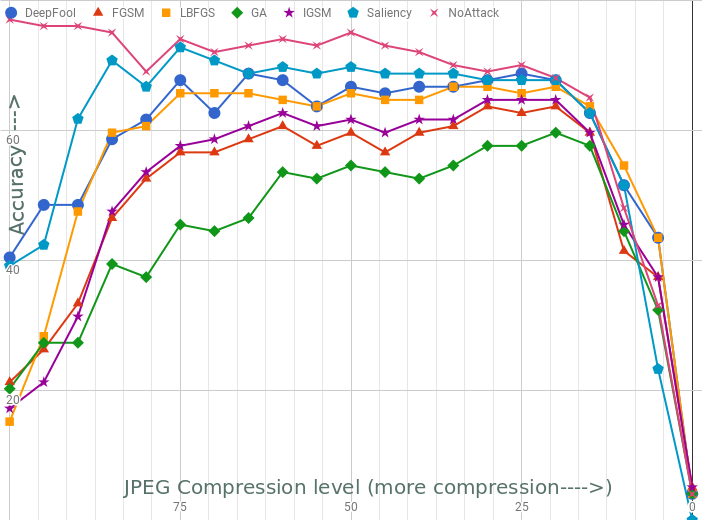
\includegraphics[width=0.46\textwidth,angle=0]{figures/protect/jpeg_study.png}
     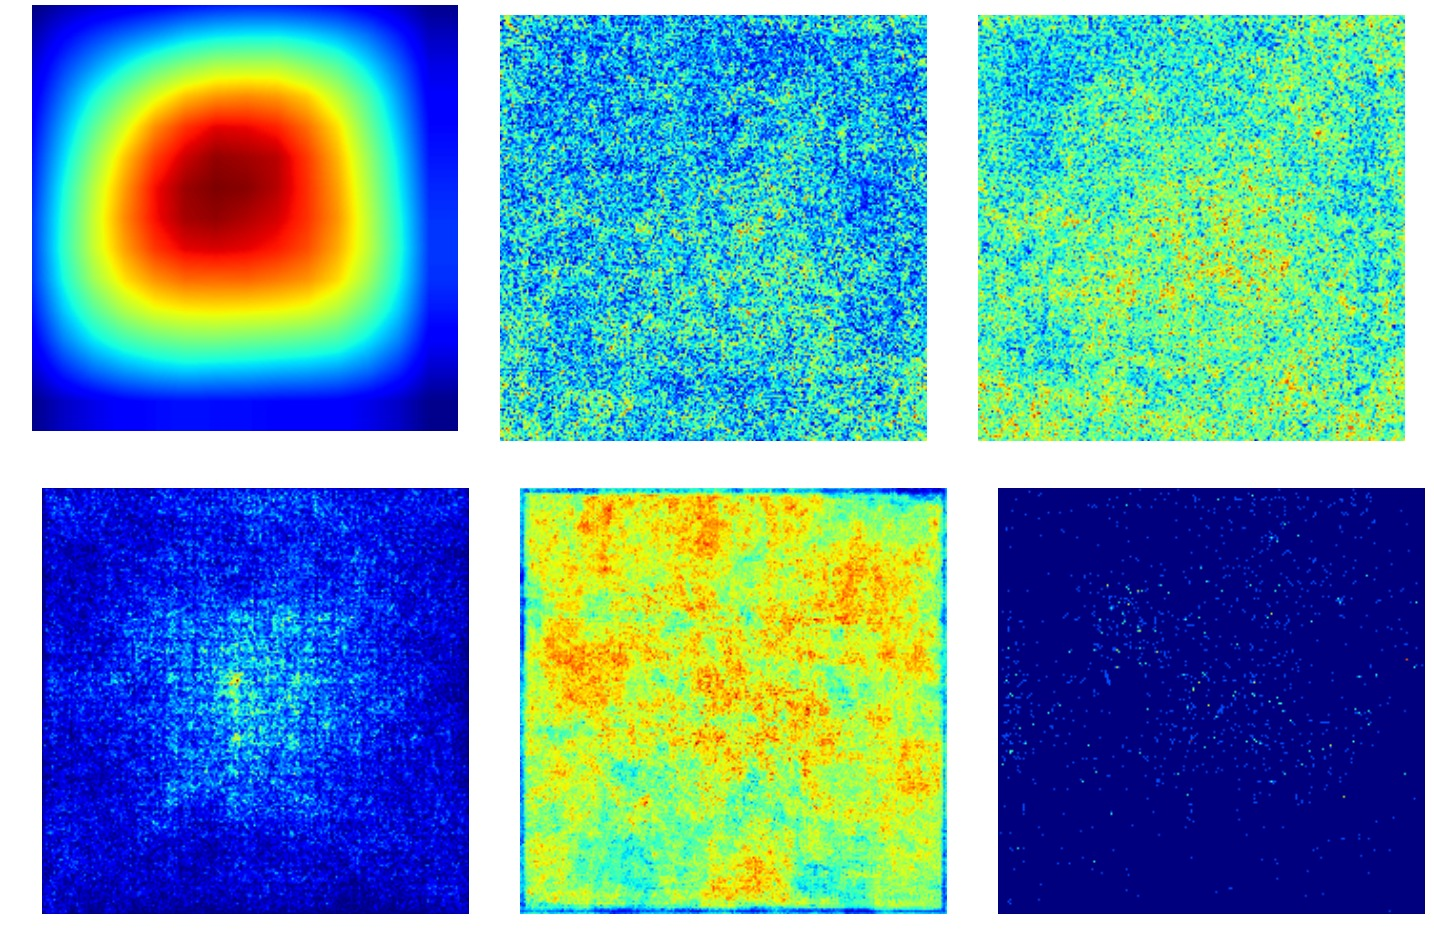
\includegraphics[width=0.52\textwidth,angle=0]{figures/protect/drawing_noise.jpg}
     %\vspace{-5mm}
     \label{fig:jpeg}
     \caption[JPEG under attack]{(a) Classification accuracy on adversarial images is recovered as quantization increases, but drops when quantization becomes too aggressive. \textit{JPEG Compression level} refers to the scaling factor of the quantization matrix often denoted as Q. (b) Clockwise from top left; average MSROI saliency map for original images, average adversarial perturbations for five attack methods (IGSM, FGSM, JSMA, Deep Fool, GA).  Note that noise intensity is not concentrated in salient regions.}
%\vspace{-5mm}
 \end{figure}
%Yet another defense against adversarial images is to either detect the presence of adversarial perturbations in the given image

%\SubSection{Transformations}


% If space remaining cite Bhagogi and discuss, data transformations like PCA.
%\vspace{-2mm}
\paragraph{Limitations of JPEG} - Recently, it has been shown that image transformations such as Gaussian blur, Gaussian noise, change of contrast and brightness, and image compression like JPEG are able to recover some portion of correct classifications when applied to adversarial images ~\cite{Kurakin2016AdversarialEI}.
The impact of JPEG compression was further studied by ~\cite{Dziugaite2016ASO} and ~\cite{Das2017KeepingTB}.
Their studies were limited to less effective attack techniques, such as FGSM, but demonstrated the baseline efficacy of JPEG. 
We show that standard JPEG does not defend against newer and more robust attacks, and analyze some of the limitations of pure JPEG for adversarial defense.

JPEG's success in defending against some attack models is due to the quantization of high-frequency signals in the image.
The high frequencies will contain some portion of the perturbations added by the attacker, and quantization will lessen their impact.
However, adversarial perturbations in lower frequencies remain, and the more aggressive quantization which is required to remove these perturbations results in lower image quality, making it difficult to recover the original classification.


%OLD
%Some portion of the adversarial perturbations lie in the high frequencies, which are strongly quantized during JPEG compression.
%Therefore, doing lossy JPEG compression gets rid of these high-frequency perturbations and reduces the impact of adversarial noise on the classification of the image.
%[TODO:DONE experiment to show this - plot histogram of adv perturbation (diff) ]
%Not all perturbations occur in same frequency, and it requires a stronger quantization (lower Q value on JPEG) to overpower all of the adversarial noise. However, this comes at a cost of losing both image quality and classification accuracy.
%END OLD

 
%Unlike adversary, a defensive model is not constrained by a $L_p$ distance, regardless of that, losing integrity of the image would mean reduced classification accuracy.

To maximize the effectiveness of our defense, while still preserving sufficient quality to allow for correct classification, we seek to strongly quantize those regions of the image which are not salient to the true class, while weakly quantizing salient regions.
We present a method for achieving this in the following section.

%\vspace{-2mm}
\section{Semantic Quantization}

Our approach employs a transformation $T(x)$ of a given image $x$ which quantizes the image in the frequency domain like standard JPEG.
However, unlike JPEG, we determine the salient regions of $x$ , i.e. regions for which the presence of an object is likely, and quantize those regions at higher bit-rates than non-salient regions.
We use a convolutional neural network to generate a saliency heat map, % RCM TODO: add citation here?
which guides quantization.

The center plot on Figure 1 shows the map of the perturbations added by an adversarial system (IGSM). The adversary has made modifications to every image region (except where the image is saturated), even though the elephant is in the center of the image. Our method takes advantage of this, and strongly quantizes the image blocks outside of the salient region. %[TODO: Maybe instead reference figure 2? It shows this more clearly]

\begin{figure}[H]
\centering
     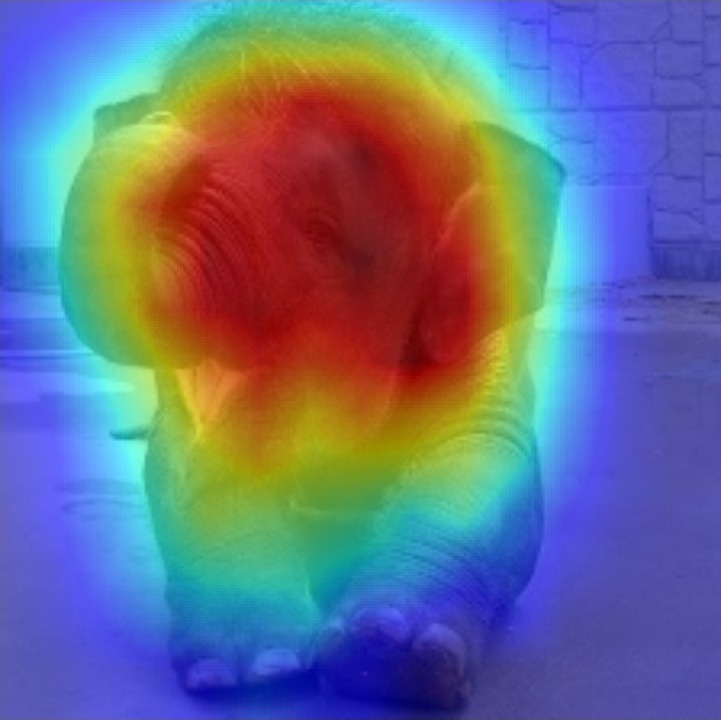
\includegraphics[width=0.3\textwidth,angle=0,scale=0.7]{figures/protect/original_msroi.jpg}
     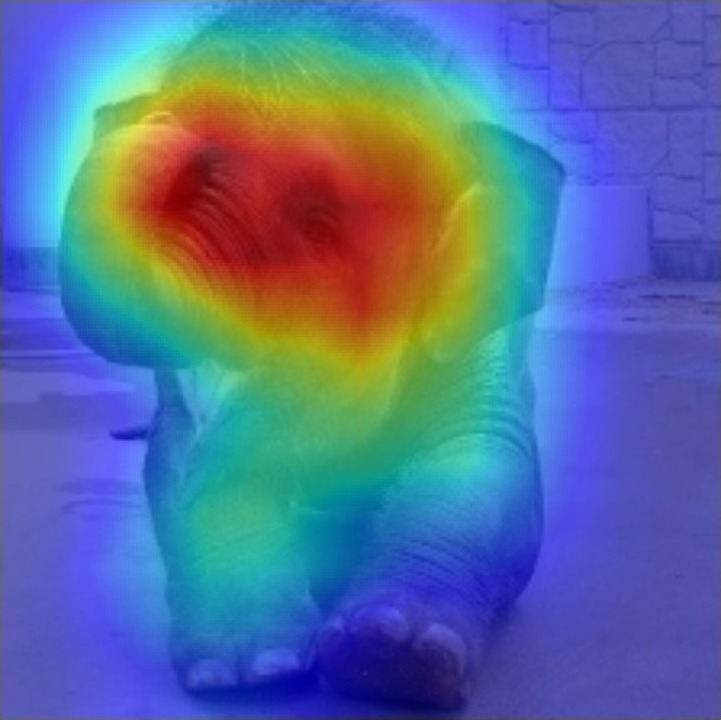
\includegraphics[width=0.3\textwidth,angle=0,scale=0.7]{figures/protect/adversarial_msroi.jpg}
     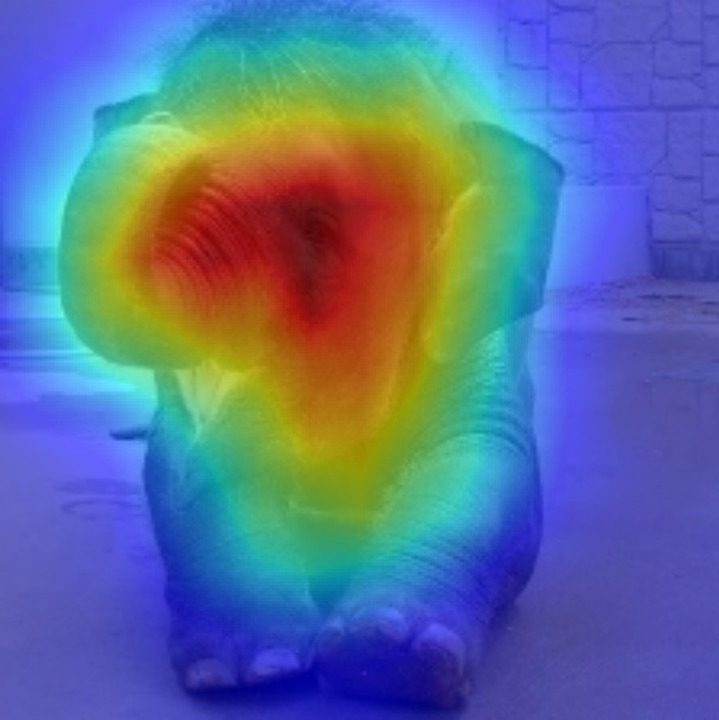
\includegraphics[width=0.3\textwidth,angle=0,scale=0.7]{figures/protect/MSROI_after.jpg}
     \label{fig:msroi}
          \caption[Multi-Structure ROI]{Left: MSROI on original image, Center: MSROI, Right: Aug-MSROI, on adversarial image}
 \end{figure}
 

Convolutional neural networks (CNNs) have been used to detect and locate objects in a given image \cite{Erhan2014ScalableOD,Zhao_2015_CVPR}. 
However, these works seek to generate a hard bounding box around the objects which does not take into consideration partial or occluded objects.
They are also limited in the number of classes they can detect, which ranges between $20$ to $40$.
%TODO: cite some saliency technique papers
Saliency detection techniques can solve these issues, but such techniques are limited in their ability to detect multiple objects, and the identified salient region may only contain a limited subset of the objects in the image.
To address these shortcomings, we utilize MSROI  ~\cite{Prakash2017SemanticPI}, a CNN designed to retrieve all salient regions and provide a soft boundary over the image.

MSROI generates a heat map based on its confidence over all classes and their corresponding activation values. 
At each layer, $l$, of the network, MSROI has independent filters for each class in the dataset. 
Thus, summing the filter responses of each class over their respective filters represents the confidence of that class. 
For an image $x$ at a given location of ($i,j$) and $C$ classes, MSROI map is defined as:

\[
M(i,j) = \sum_{c \in C} \begin{cases}
                        \sum_l f_l^c(i,j) & \text{if} \sum_{l} \sum_{x,y} f_d^c(i,j) > \mathcal{T} \\
                        0 & \text{otherwise}
                        \end{cases}
\]

\begin{figure}[H]
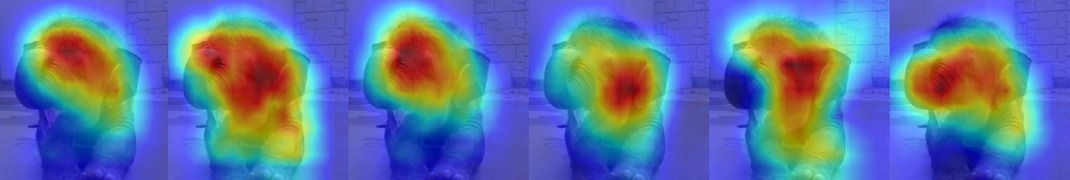
\includegraphics[scale=0.4]{figures/protect/out2_small_small.png}
           %\vspace{-3mm} 
     \label{fig:combination}
          \caption[Combination of various jittered inputs]{Combination of various jittered inputs}
          %\vspace{-6mm} 
 \end{figure}


%[TODO: briefly explain about images being centered]
When the confidence of the model on a specific class is below a threshold $\mathcal{T}$ (determined through experimentation on validation data), the class is not represented. 

%\vspace{-2mm}
\section{Augmented MSROI}
%[TODO: explain weighting/ difference from standard MSROI]
MSROI was trained on natural images, but in this task it will be applied to an adversarial image. 
This means that the incorrect adversarial classification will be represented in the saliency map.
This presents an issue, as the adaptive quantization will try to preserve those areas which are salient to the incorrect classification. 
Thus, performing standard MSROI retains some adversarial noise which could have been quantized away.
To counteract this, we augment the MSROI algorithm by generating several small random perturbations of the image and the intermediate activations of the MSROI network, and calculating a saliency map $\widetilde{M}$ for each such perturbation:
%\vspace{-2mm}
\[
\widetilde{M}(i,j) = \sum_{c \in \hat{C}}  \sum_l (a_l^c(i ,j))  \text{\quad and \quad} a_{l+1}^c = f_l(a_l^c(i,j) +\Delta)
%\vspace{-2mm}
\]
where $\Delta$ is a random perturbation and $\hat{C}$ is subset of $C$ found similarly using $\mathcal{T}$ as shown with MSROI.
We take an average of $\widetilde{M}$ maps over several perturbations to generate a final map, which we term Augmented MSROI (Aug-MSROI).
This process of averaging over many perturbations gives softer localization which is less vulnerable to attack.
%The ($i,j$) signifying the most salient objects gets adds over many times, thereby making the localization of object less precise but more robust.%TODO: FIXME
The number of perturbations to average over can be found empirically.  %[TODO DONE fix this sentence]
%TODO: these figures are causing question marks ??
Figure 4 shows several individual $\widetilde{M}$ maps which are combined to create the final heat map. 
In Figure 3 we show the difference between standard MSROI and Aug-MSROI. 
Most of the head of the baby elephant is retrieved in the Aug-MSROI heat map but not in the standard MSROI. 
%REMOVED BELOW - this is explained at the start of this section
%Computation of MSROI relies heavily on the most prominent class even if it was designed to find all salient objects.
%Since an adversarial image's top-1 prediction has changed, it changes the saliency map built by MSROI.

Once the semantic heat map is obtained, we use the technique proposed in \cite{Prakash2017SemanticPI}, which quantizes different $8\times8$ blocks at different levels and combines them to obtain a final JPEG image. 
This final image retains high quality in salient regions, and is heavily quantized in non-salient regions.
Strong quantization in non-salient regions is often sufficient to reverse the impact of adversarial perturbations, and high quality in salient regions allows recovery of the correct classification.
%The map has to be discretized so that different levels of quantization can be applied. 
%We bin the heat map into $K$ different levels.
%We then pick $K$ different tables for quantization of these blocks. 
%For simplicity we use different scaling factor on the same table, values of which were obtained from JPEG standard \cite{wallace1992jpeg}, but these tables could be different from each other, as different quantization tables exist for JPEG blocks \cite{wang2001designing}.
%This was done to keep the comparison against JPEG as fair as possible. After the quantization, inverse DCT is performed for each block. 


%[TODO DONE: note that AugMSROI is standard JPEG decodable, small increase in encoding cost]
Our modifications of the standard MSROI algorithm result in only a modest increase in encoding complexity, and, like standard MSROI, the resulting compressed image can be decompressed by a standard off-the-shelf JPEG decoder.
Even though JSMA and L-BFGS attack selected pixels, the pixels changed by these attacks do not significantly correlate with the pixels selected by Aug-MSROI. Aug-MSROI extracts pixels belonging to the object while JSMA extracts pixels most likely to cause the change in image classification, which often lie in the negative space.

%\SubSection{Quantization}
%Once the semantic heat map is obtained we bin the heat map into $K$ slots. 
%Every $8\times8$ block of the original image is then compressed using JPEG encoder at different quantization levels.
%Then the frequency components are quantized based on the values on the saliency map.

%\vspace{-2mm}
\section{Experiments}

We experimented with several adversarial attacks as described in Section ~\ref{attacks}.
We used Residual Network (ResNet-50) ~\cite{He2016DeepRL}, a state-of-the-art deep CNN as the classification model. 
Our test images are scaled and cropped to $256 \times 256$, and are drawn from the ImageNet dataset, which contains $1000$ classes.
%ResNet-50 is a fifty layer deep neural network which consists of convolutional layers with skip connections \cite{He2016DeepRL}.
%This has been shown to improve classification accuracy considerably \cite{He2016IdentityMI}
%VGG-19 is comparatively less accurate but is known to generalized well in image transfer applications. \cite{Simonyan2014VeryDC}.
% If space is limited consider removing lines about resnet & vgg
All the attacks were parametrized to have RMSE distance of $0.02$ compared to the original image.
Aug-MSROI, like MSROI, requires a one-time off-line training of the model. Encoding of images can be done in parallel for several images on a GPU. Computation of Aug-MSROI map requires multiple perturbations for the same image and thus is somewhat more resource intensive than computing MSROI map. However, these passes can be computed in parallel as the final map is an average of individual maps. On a Titan X Maxwell GPU with 12 GB of memory encoding 300 images, each with five perturbations, took 5 seconds total; the decoding process remains unchanged from standard JPEG.
%We compare our results against the original MSROI technique, as well as off-the-shelf JPEG. 
%[TODO add the graph showing JPEG destruction rate at different Q level.] 

%\vspace{-2mm}
\paragraph{Metrics for comparison} Accuracy is the most common metric for assessing performance of deep neural networks on image classification tasks.
Most publications report `Top-5' accuracy, which is calculated by counting the number of instances for which the image's true label is in the top five predicted labels. 
For the purposes of adversarial attacks, we consider an attack to be successful if the model's top predicted class $c'$ for adversarial image $x'$ is not the same as the top predicted class for the original image $x$ i.e `Top-1' accuracy. 
This is a very generous success metric for the adversary, as the predicted class label for most of the adversarial images are within the `Top-5' of the original image even if not in `Top-1'.

We achieved 76\% accuracy with Residual Network (ResNet-50), which is in accordance with the reported numbers \cite{He2016DeepRL}.
In other words, after applying our defense, we recover a level of classification accuracy which is close to the accuracy obtained on non-adversarial images.
Since the top-1 accuracy of classifier on the original image is limited the metric is biased towards adversary because in many cases adversary does not even have to work to produce a success.


Therefore, to measure the effectiveness of a transformation, $T$, we also report destruction rate as proposed in \cite{Kurakin2016AdversarialEI}. 
Destruction rate is fraction of adversarial images which are no longer misclassified after the transformation. 

Let $C$ be a function defined as -

\[
C(x,y) = \begin{cases}
  1, & \text{if image $x$ is classified as $y$} \\
  0, & \text{otherwise}
\end{cases}
\]
Then, destruction rate is defined as --
\[
d = \frac{\sum_{i=1}^N C(x_i, y_i) \times (1 - C(x'_i,y)) \times C(T(x'_i),y_i)}{\sum_{i=1}^N C(x_i, y_i) \times (1 - C(x'_i,y))}
\]


\begin{figure}[H]
   \centering
     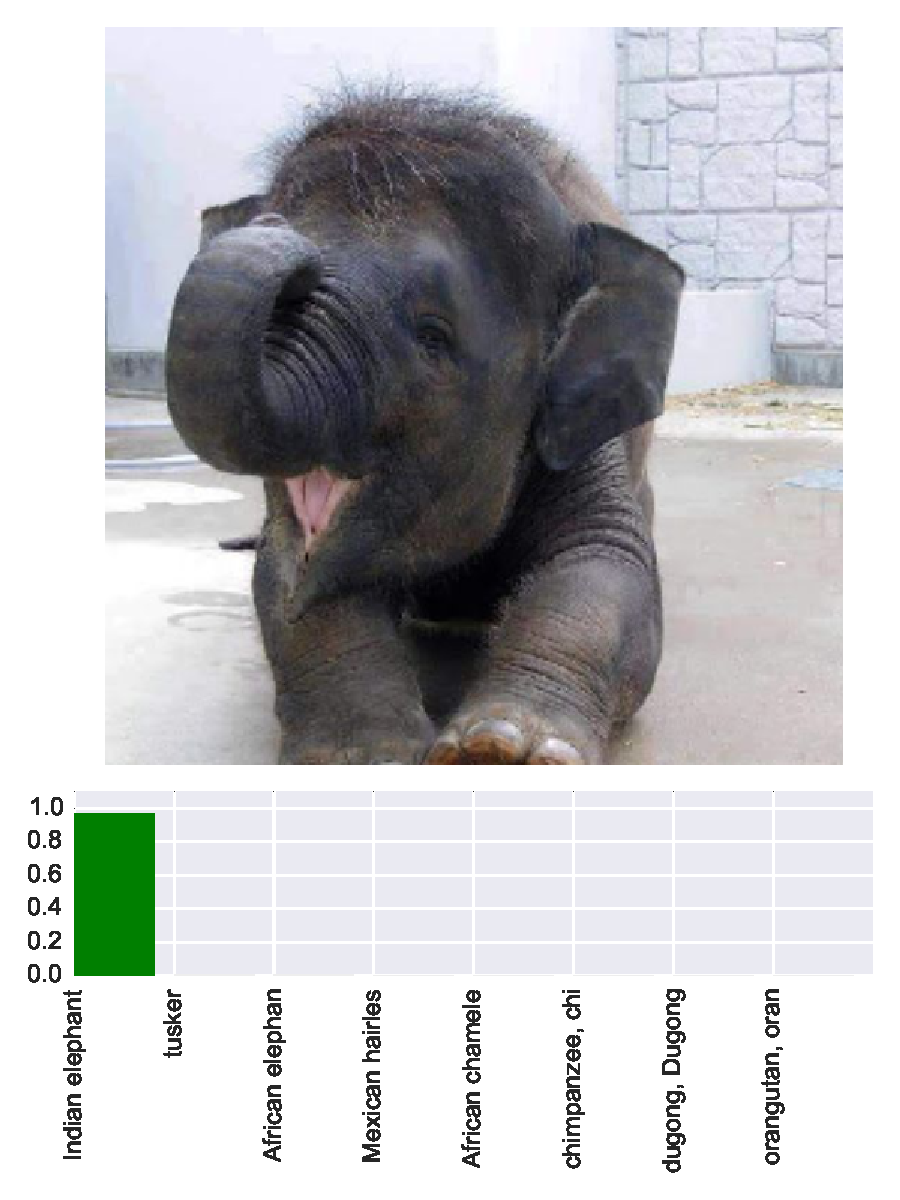
\includegraphics[width=0.24\textwidth,angle=0]{figures/protect/ori.pdf}
     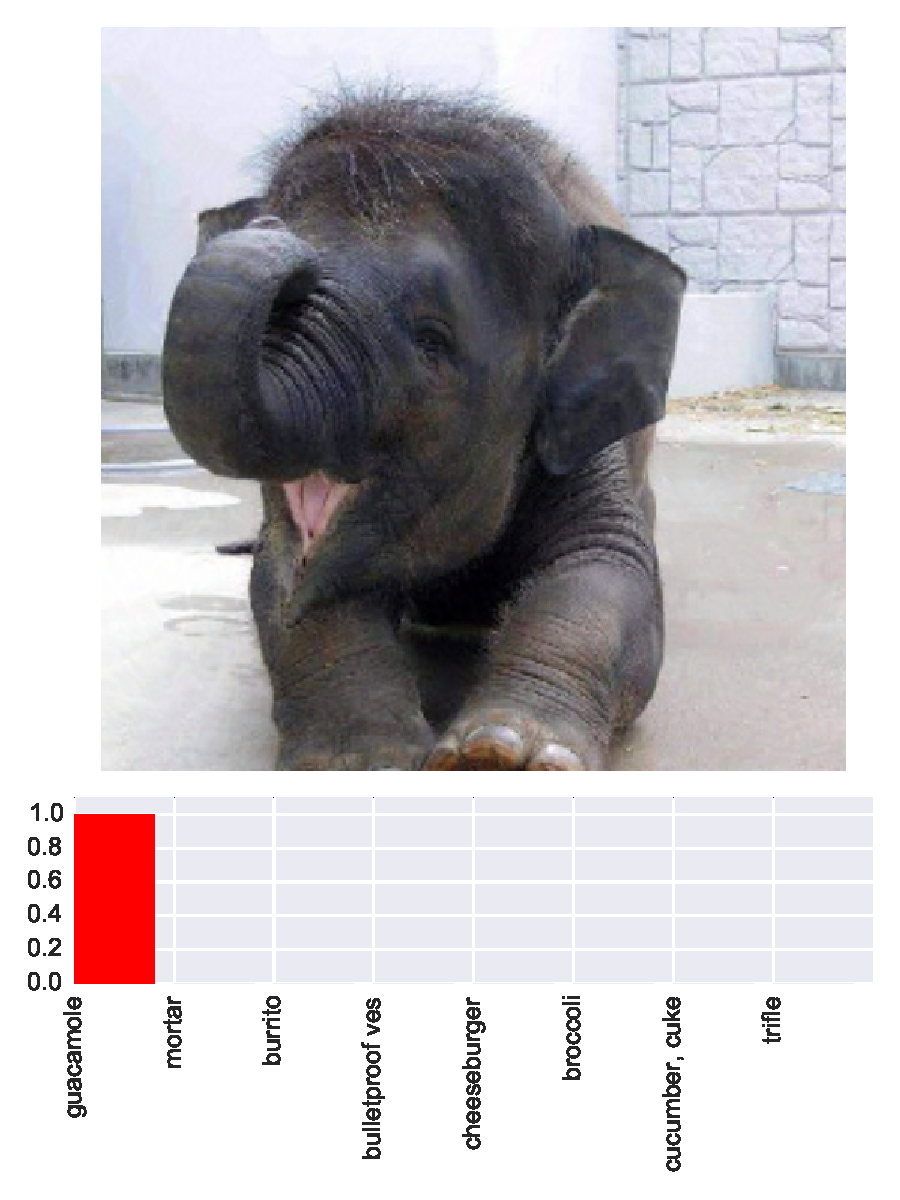
\includegraphics[width=0.24\textwidth,angle=0]{figures/protect/adv.pdf}
     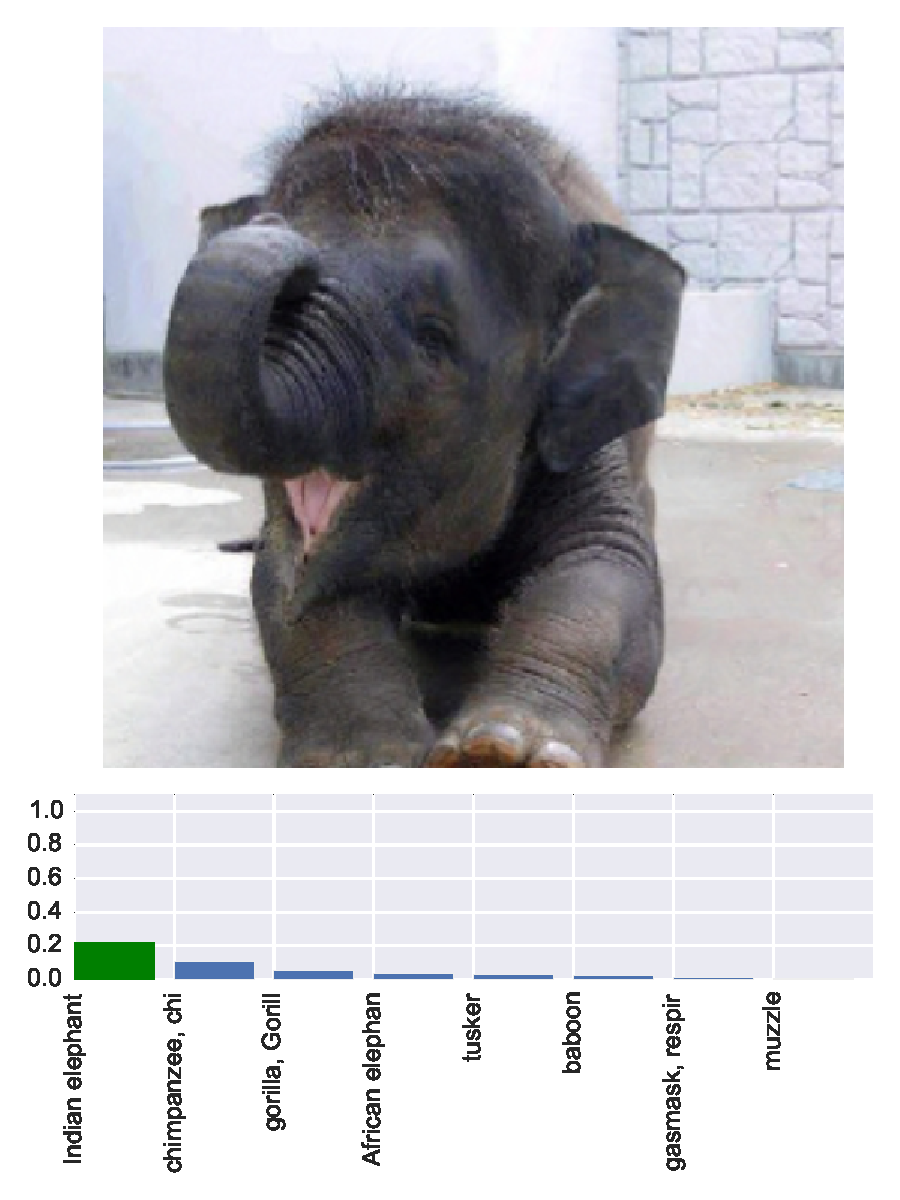
\includegraphics[width=0.24\textwidth,angle=0]{figures/protect/jpg.pdf}
     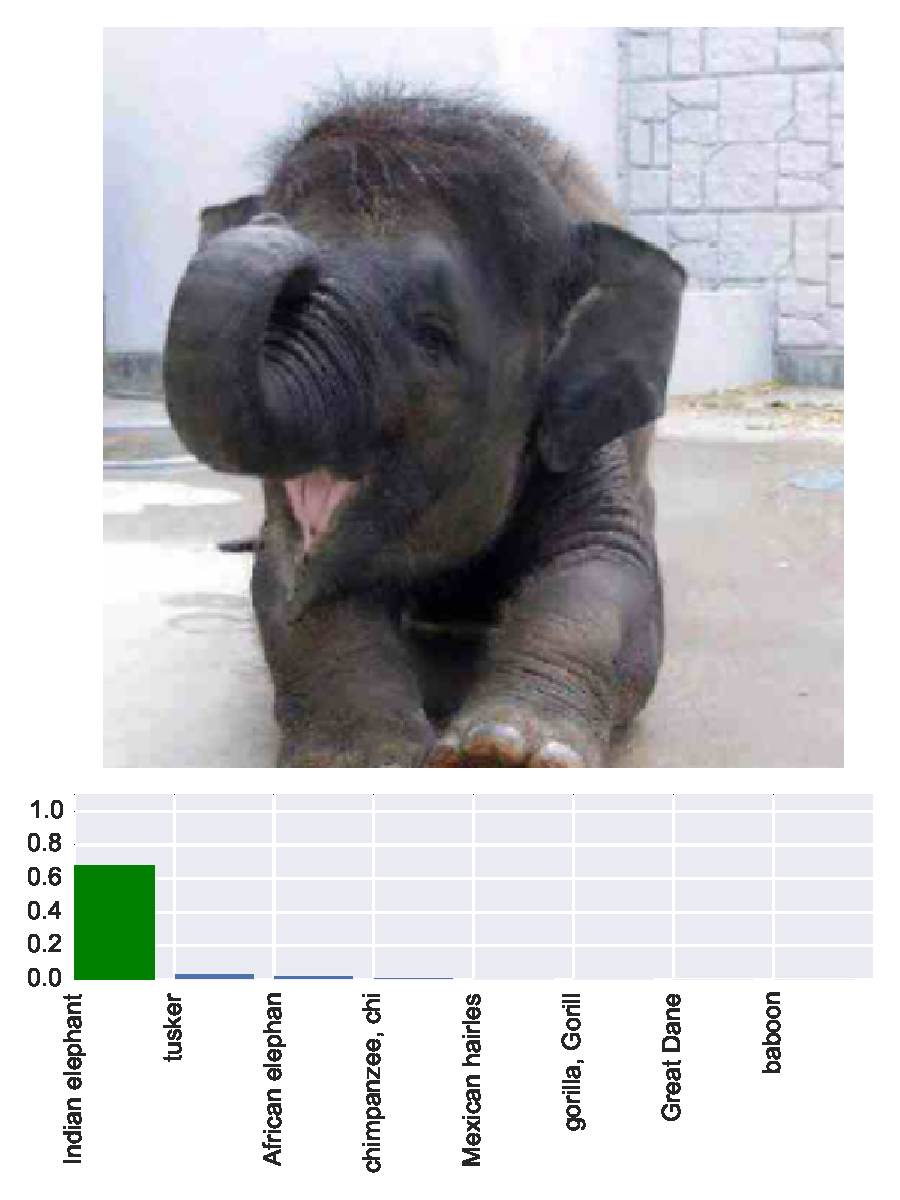
\includegraphics[width=0.24\textwidth,angle=0]{figures/protect/msroi.pdf}
          %\vspace{-4mm} 
              \caption[Augmented Multi-Structure ROI]{Original Image, Adversarial Image, JPEG, Aug-MSROI }
     \label{fig:compare}
          %\vspace{-4mm} 
 \end{figure}
 
 
 \begin{figure}[H]
     \centering
     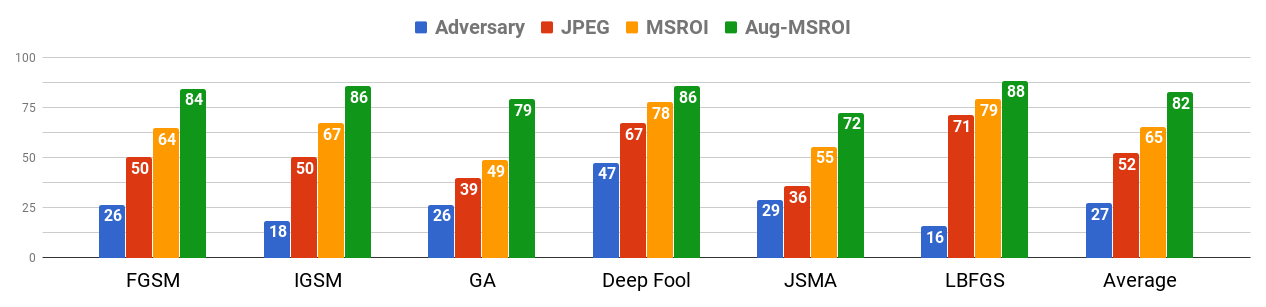
\includegraphics[width=0.99\textwidth,angle=0]{figures/protect/results.png}
     %\vspace{-5mm} 
     \caption[Classification accuracy of images on various attacks]{Classification accuracy of images on various attacks}
     \label{fig:numbers}
     \end{figure}

%\vspace{-2mm}
\section{Results}
Figure ~\ref{fig:compare} shows a typical example of the results for qualitative comparison. In this case, while JPEG was also able to retrieve the original class, it does so with significantly lower confidence. 
Table 1 shows the quantitative results averaged across 300 images of ImageNet.

\begin{table}[H]
\centering
\label{tbl:results}
%%\vspace{-10pt} 
\rowcolors{1}{White}{Gray}
\begin{tabular}{rclll}
\multicolumn{1}{l}{} & \textbf{Accuracy$\uparrow$} & \textbf{MSE$\downarrow$} & \textbf{SSIM$\uparrow$} & \textbf{PSNR$\uparrow$} \\ \hline
\textbf{JPEG}        & 52                & 16.55        & 0.62          & 24.33         \\
\textbf{MSROI}       & 65                & 16.13        & 0.64          & 24.61         \\
\textbf{Aug-MSROI}   & 82                & 10.92        & 0.86          & 27.36        
\end{tabular}
%\vspace{-10pt} 
\caption[Quantitative results using Aug-MSROI]{Results averaged across $300$ images. }
%\vspace{-10pt} 
\end{table}
 

The JPEG quantization level was chosen to achieve the highest accuracy. 
For MSROI, we applied the technique described in ~\cite{Prakash2017SemanticPI} and set the quantization level to keep the final image quality as close as possible to the JPEG version. The results are shown in Figure 2(a). %RCM TODO, maybe use a label?  % RCM TODO this makes it sound like you matched the quality of the MSROI to the best JPEG, instead of leaving the quality fixed -- is that the case?
Aug-MSROI improved classification accuracy while maintaining the perceptual quality as evaluated by PSNR, MSE and SSIM ~\cite{wang2004image}. %TODO: reference for SSIM

%\vspace{-2mm}
\section{Conclusion}

%We explored various vulnerabilities of neural networks against adversarial attacks. We investigated efficacy and limitations of standard JPEG and semantic JPEG against these minute perturbations. We proposed a variant of semantic quantization which is robust against adversarial perturbation. Our experiments show that such a model is able to recover significant amount of images. Compared to other defense techniques which require learning a new model, our method can be carried out as a image processing step. Images generated by our technique can easily be decoded by any standard JPEG decoder. 

We have presented Aug-MSROI, an augmentation of MSROI ~\cite{Prakash2017SemanticPI}  to employ semantic JPEG compression as an effective defense against state-of-the-art adversarial attacks.
In our experiments, JPEG compression employing Aug-MSROI produces compressed images, which, when decompressed, have high visual quality while at the same time preserving the accuracy of classification by a neural network. 
A key advantage of our approach is that, with only a modest increase in encoding time, like standard MSROI, it produces compressed images that can be decompressed by any off-the-shelf JPEG decoder.


\chapter{Pixel Deflection}
\section{Introduction}


Image classification convolutional neural networks (CNNs) have become a part of many critical real-world systems.
For example, CNNs can be used by banks to read the dollar amount of a check ~\cite{Bottou1997GlobalTO}, or by self-driving cars to identify stop signs ~\cite{Papernot2016PracticalBA}.%DONE: citations?

The critical nature of these systems makes them targets for adversarial attacks.
Recent work has shown that classifiers can be tricked by small, carefully-crafted, imperceptible perturbations to a natural image.
These perturbations can cause a CNN to misclassify an image into a different class (\eg a ``1'' into a ``9'' or a stop sign into a yield sign). 

Thus, defending against these vulnerabilities will be critical to the further adoption of advanced computer vision systems.
Here, we consider \emph{white-box} attacks, in which an adversary can see the weights of the classification model.
Most of these attacks work by taking advantage of the differentiable nature of the classification model, \ie taking the gradient of the output class probabilities with respect to a particular pixel. 
Several previous works propose defense mechanisms that are differentiable transformations applied to an image before classification.
These differentiable defenses appear to work well at first, but attackers can easily circumvent these defenses by ``differentiating through them'', \ie by taking the gradient of a class probability with respect to an input pixel through both the CNN and the transformation. 

In this work, we present a defense method which combines two novel techniques for defending against adversarial attacks, which together modify input images in such a way that is (1) non-differentiable, and (2) frequently restores the original classification.
The first component, \emph{pixel deflection}, takes advantage of a CNN's resistance to the noise that occurs in natural images by randomly replacing some pixels with randomly selected pixels from a small neighborhood.
We show how to weight the initial random pixel selection using a \emph{robust activation map}.
The second approach, \emph{adaptive soft-thresholding} in the wavelet domain, which has been shown to effectively capture the distribution of natural images.
This thresholding process smooths adversarially-perturbed images in such a way so as to reduce the effects of the attacks.

Experimentally, we show that the combination of these approaches can effectively defend against state-of-the-art attacks ~\cite{Szegedy2013IntriguingPO, Goodfellow2014ExplainingAH,Carlini2017TowardsET,MoosaviDezfooli2016DeepFoolAS,papernot2016limitations,Kurakin2016AdversarialEI}
%DONE: List of citations
Additionally, we show that these transformations do not significantly decrease the classifier's accuracy on non-adversarial images.

In Section ~\ref{sec:advattacks}, we discuss the various attack techniques against which we will test our defense.  In Sections ~\ref{sec:defenses} and ~\ref{sec:related} we discuss the established defense techniques against which we will compare our technique.  In Sections ~\ref{sec:pdrop}, ~\ref{sec:tpd} and ~\ref{sec:wavelet} we lay out the components of our defense and provide the intuition behind them.  In Sections ~\ref{sec:exp} and ~\ref{sec:results_pixel}, we provide experimental results on a subset of ImageNet.

%TODO: fill in



We propose a two-step process to defend against adversarial attacks on existing networks.

\begin{enumerate}
\item Apply targeted \textit{pixel deflection} guided by robust activation maps, as described in Sections ~\ref{sec:pdrop} and ~\ref{sec:tpd}.
\item Apply adaptive soft thresholding to the image in a wavelet domain, as described in Section ~\ref{sec:wavelet}.
\end{enumerate}

In a white-box attack model, the adversary is able to find the gradient of the image pixels with respect to the classification error.  
In this paradigm, defenses which employ a differentiable transformation are of limited effectiveness, as the adversary can simply incorporate that transformation into their training.
Our method avoids this potential weakness by applying a non-differentiable transformation which stochastically alters pixel values.
These factors reduce the adversary to working in a gray-box environment, in which gradients can only be computed for part of the classification process, and in which the adversary cannot be certain which perturbations will be preserved.

Previously proposed defenses which rely on a strong quantization ~\cite{Dziugaite2016ASO,Das2017KeepingTB} are often successful at avoiding the adversarial class, but this success comes at the cost of decreased performance on clean images.
By contrast, our method uses an adaptive quantization scheme which preserves the classification of clean images at a much higher rate.
Defenses which are based around a deterministic, differentiable transformation are of limited effectiveness, as the adversary can simply incorporate that transformation into their training.
It is difficult to incorporate our technique as a an augmentation process for adversarial loss, because it decreases the space and availability of pixels for the attack.


White-box attacks are based on the ability to find the gradient of image with respect to the classification error. 
Our defense technique stochastically changes the pixel values, in a way which is non-differentiable, thereby reducing a white-box attack to a grey-box attack.

%Most denoising based defense methods ~\cite{Dziugaite2016ASO,Das2017KeepingTB} come at cost of reduced accuracy of the classifier on the clean images.
This is a limitation of hard and fixed quantization. 
Our method uses adaptive and soft quantization and therefore, accuracy of clean images remains unchanged.





\section{Adversarial Attacks\label{sec:advattacks}}
%RYAN
It has been established that most image classification models can easily be fooled ~\cite{Szegedy2013IntriguingPO,Goodfellow2014ExplainingAH}. 
Several techniques have been proposed which can generate an image that is perceptually indistinguishable from another image but is classified differently. 
This can be done robustly when model parameters are known, a paradigm called \textit{white-box attacks} ~\cite{Goodfellow2014ExplainingAH,Kurakin2016AdversarialEI,Madry2017TowardsDL,Carlini2017TowardsET}.
In the scenario where access to the model is not available, called \textit{black-box attacks}, a secondary model can be trained using the model to be attacked as a guide.
It has been shown that the adversarial examples generated using these substitute models are transferable to the original classifiers ~\cite{Papernot2016PracticalBA,Liu2016DelvingIT}.

Consider a given image $x$ and a classifier $F_\theta(\cdot)$ with parameters $\theta$.
%Then an adversarial example for $x$ is an image $\hat{x}$ such that, under a certain $L_P$ norm, they are very close (\ie $||x-\hat{x}||_{L_P}$ is small),  but the classifier's prediction for each of them is different, \ie $F(x) \neq F(\hat{x})$. 
Then an adversarial example for $F_\theta(\cdot)$ is an image $\hat{x}$ which is close
% RYAN I just removed the L_P to make it just any old norm
to $x$ (\ie $||x-\hat{x}||$ is small, where the norm used differs between attacks),  but the classifier's prediction for each of them is different, \ie $F(x) \neq F(\hat{x})$. 
% RYAN plural "attack"
\textit{Untargeted attacks} are  methods to produce such an image, given $x$ and $F_\theta(\cdot)$. 
%As long as the model mis-classifies $\hat{x}$, the attack is considered a success.
%Such attacks are called , in which the value of $F(\hat{x})$ is unconstrained beyond the requirement that it differ from $F(x)$.
%A stronger form of an attack is a {targeted attack}, in which the attacker is given $x$, $F(\cdot)$, and a specific target class $\hat{y}$, and produces $\hat{x}$ such that $F(\hat{x}) = \hat{y} \neq F(x)$.
%RYAN untargeted => targeted, also made structural parallel
\emph{Targeted attacks}, however, seek a $\hat{x}$ such that $F(\hat{x}) = \hat{y}$ for some specific choice of $\hat{y} \neq F(x)$, i.e. targeted attacks try to induce a specific class label, whereas untargeted attacks simply try to destroy the original class label.

% RYAN phrasing
Next, we present a brief overview of several well-known attacks, which form the basis for our experiments.

% RYAN reordered, but FGSM and IGSM next to each other
\subsection{Fast Gradient Sign Method (FGSM)}
\cite{Goodfellow2014ExplainingAH} is a single step attack process.
It uses the sign of the gradient of the loss function,  $\ell$,  with respect to to the image to find the adversarial perturbation. 
For a given value $\epsilon$, FGSM is defined as:
\begin{equation}
\hat{x} = x + \epsilon \text{sign} (\nabla \ell (F(x),x))
\end{equation}

\subsection{Iterative Gradient Sign Method (IGSM)} 
\cite{Kurakin2016AdversarialEI} is an iterative version of FGSM. After each iteration the generated image is clipped to be within a $\epsilon L_\infty$ neighborhood of the original and this process stops when an adversarial image has been discovered. 
Both FGSM and IGSM minimize the $L_\infty$ norm with respect to to the original image. Let $x_0' = x$, then after $m$ iterations, the adversarial image is obtained by:
\begin{equation}
x_{m+1}' = \text{Clip}_{x,\epsilon} \Bigl\{x_m' + \alpha \times \text{sign}(\nabla \ell (F(x'_m),x'_m))  \Bigr\} 
\end{equation}

\subsection{L-BFGS} ~\cite{Szegedy2013IntriguingPO} tries to find the adversarial input as a box-constraint minimization problem.
L-BFGS optimization is used to minimize $L_2$ distance between the image and the adversarial example while keeping a constraint on the class label for the generated image.
%This is a slow and iterative targeted attack which generally produces images with small perturbations and strong classifier confidence in the misclassification.


\subsection{Jacobian-based Saliency Map Attack (JSMA)} 
\cite{papernot2016limitations} estimates the saliency of each image pixel with respect to to the classification output, and modifies those pixels which are most salient. This is a targeted attack, and saliency is designed to find the pixel which increases the classifier's output for the target class while tending to decrease the output for other classes.

\subsection{Deep Fool (DFool)}
 ~\cite{MoosaviDezfooli2016DeepFoolAS} is an untargeted iterative attack. 
This method approximates the classifier as a linear decision boundary and then finds the smallest perturbation needed to cross that boundary.
This attack minimizes $L_2$ norm with respect to to the original image. 

\subsection{Carlini \& Wagner (C\&W)}
 ~\cite{Carlini2017TowardsET} is a recently proposed adversarial attack, and one of the strongest.
%RYAN what loss function? Is this an explanation ppl in CV will understand? 
C\&W updates the loss function, such that it jointly minimizes $L_p$ and a custom differentiable loss function that uses the unnormalized outputs of the classifier (\textit{logits}). 
Let $Z_k$ denote the logits of a model for a given class $k$, and $\kappa$ a margin parameter. Then C\&W tries to minimize:
\begin{equation}
|| x - \hat{x} ||_p + c* max\left(Z(\hat{x}_y) - max\{Z(\hat{x})_k : k \neq y\},-\kappa\right)
\end{equation}
For our experiments, we use $L_2$ for the first term, as this makes the entire loss function differentiable and therefore easier to train. 
Limited success has been observed with $L_0$ and $L_\infty$ for images beyond CIFAR and MNIST.

We have not included recently proposed attacks like `Projected Gradient Descent' ~\cite{Madry2017TowardsDL} and `One Pixel Attack' ~\cite{Su2017OnePA} because although they have been shown to be robust on datasets of small images like CIFAR10 and MNIST, they do not scale well to large images. 
Our method is targeted towards large natural images where object localization is meaningful, i.e. that there are many  pixels outside the region of the image where the object is located.

%TODO, maybe PGD.

\section{Defenses\label{sec:defenses}}

%When an image is provided, which may or may not have adversarial perturbations, the goal of the defense method is to classify the images with same predictions.
%If $F(x)=F(\hat{x})$ then defense is considered as successful. 
%Defense strategies are based on either building a robust classifier such that it is harder to find an adversarial example, or they are based on some transformation $\mathcal{T}$ such that $F(\mathcal{T}(\hat{x}))=F(\mathcal{T}(x))=F(x)$. 
Given a classification model $F$ and an image $\tilde{x}$, which may either be an original image $x$, or an adversarial image $\hat{x}$, the goal of a defense method is to either augment either $F$ as $F'$ such that $F'(\tilde{x}) = F(x)$, or transform $\tilde{x}$ by a transformation $\mathcal{T}$ such that $F(\mathcal{T}(\tilde{x}))=F(x)$.

One method for augmenting $F$ is called Ensemble Adversarial training ~\cite{Tramr2017EnsembleAT},  which augments the training of  deep convolutional networks to include various potential adversarial perturbations. 
This expands the decision boundaries around training examples to include some nearby adversarial examples, thereby making the task of finding an adversary within a certain $\epsilon$ harder than conventional models.
Another popular technique uses distillation from a larger network by learning to match the 
%RYAN is "to match the softmax" clear, or does this need to say "to match the softmax output layer"?
softmax ~\cite{Papernot2016DistillationAA}.
This provides smoother decision boundaries and thus makes is harder to find an adversarial example which is imperceptible.
There are methods that proposes to detect the adversarial images as it passes through the classifier model ~\cite{Meng2017MagNetAT,akhtar2017defense}.

Most transformation-based defense strategies suffer from accuracy loss with clean images  ~\cite{Dziugaite2016ASO,Kurakin2016AdversarialEI}, \ie they produce $F(\mathcal{T}(x)) \neq F(x)$.
This is an undesirable side effect of the transformation process, and we propose a transformation which tries to minimize this loss while also recovering the classification of an adversarial image. 
Detailed discussion on various kinds of transformation based defenses is provided in section ~\ref{sec:related}.

%Model based defenses:
%1. Feature Squeezing \cite{FeatureSqueezingXu2017}
%TODO:
\section{Related Work \label{sec:related}}

Transformation-based defenses are a relatively recent and unexplored development in adversarial defense. 
The biggest obstacle facing most transformation-based defenses is that the transformation degrades the quality of non-adversarial images, leading to a loss of accuracy.
%Most transformations results in some undesirable loss of accuracy on clean images. 
%Thus, transformations are not considered to be a strong defense against adversarial systems.
This has limited the success of transformations as a practical defense, as even those which are effective at removing adversarial transformations struggle to maintain the model's accuracy on clean images.
%TODO: Guo et al needs a cite
Our work is most similar to Guo ~\etal's ~\cite{CounteringAIGuo17} recently proposed transformation of image by quilting and Total Variance Minimization (TVM). 
%Image quilting is the technique of patching regions of image from different source.
Image quilting is performed by replacing patches of the input image with similar patches drawn from a bank of images.
They collect one million image patches from clean images and use a $k$-nearest neighbor algorithm to find the best match.
Image quilting in itself does not yield satisfactory results, so it is augmented with TVM.
In Total Variance Minimization, a substitute image is constructed by optimization such that total variance is minimized.
Total variation minimization has been widely used ~\cite{Getreuer2012RudinOsherFatemiTV} as an image denoising technique. 
%In section ~\ref{sec:results_pixel} we have compared the results. 
Our method uses semantic maps to obtain a better pixel to update and our update mechanism does not require any optimization and thus is significantly faster.

Another closely related work is from Luo \etal ~\cite{FoveationbasedMALuo2015}. They propose a foveation-based mechanism.
% RYAN I rewrote this sentence... I'm not sure this is good, though.
%They obtain ground-truth data about object coordinates, and then crop the image to and scale the image back to the same dimensions.
Using ground-truth data about object coordinates, they crop the image around the object, and then scale it back to the original size.

%RYAN old: Our model makes is based on similar hypothesis that not all regions of the image are equally important for a classifier.
Our model shares the hypothesis that not all regions of the image are equally important to a classifier.
%However, we take a different approach to hardening an image such that salient parts are more representative of the image.
Further, foveation-based methods can be fooled by finding an adversarial perturbation within the object bounding box.
Our model does not rely on a ground-truth bounding box, and the stochastic nature of our approach means that it is not restricted to only modifying a particular region of the input.

Yet another similar work is from Xie ~\etal ~\cite{MitigatingAnon208}, in which they pad the image and take multiple random crops and evaluate ensemble classification. 
This method utilizes the randomness property that our model also exploits. 
However, our model tries to spatially define the probability of a presence of a perturbation and subsequently uses wavelet-based transform to denoise the perturbations.




\section{Pixel Deflection \label{sec:pdrop}}

Much has been written about the lack of robustness of deep convolutional networks in the presence of adversarial inputs ~\cite{EasilyFNguyen2015DeepNN,IntriguingSzegedy2013}.
However, most deep classifiers are robust to the presence of natural noise, such as sensor noise ~\cite{DirtyPODiamond2017}. 

We introduce a form of artificial noise and show that most models are similarly robust to this noise.
We randomly sample a pixel from an image, and replace it with another randomly selected pixel from within a small square neighborhood.  We also experimented with other neighborhood types, including sampling from a Gaussian centered on the pixel, but these alternatives were less effective.
 


%The process of pixel deflection, as formalized in Algorithm ~\ref{alg:swap}, results in a similar distortion to those caused by natural noise sources.
%DONE change Algorithm 1 to a real reference
% RYAN: I agree with the TODOs below very strongly. This currently reads as an extremely ad-hoc procedure with a small experiment to show it doesn't *not* work

%TODO:IMP does the above assertion need to be justified?
%TODO: Imp, give some range here, once the figure is plotted.
%We will use the term \textit{pixel dropout} to signify loss of certain percentage of pixels from the image. 
%TODO: Move notational definitions either into the algorithm box, or after it?
%TODO: justify square neighborhood as simple, efficient alternative to gaussian
We term this process \textit{pixel deflection}, and give a formal definition in Algorithm ~\ref{alg:swap}.
Let $R^r_{p}$ be a square neighborhood with apothem $r$ centered at a pixel $p$.
Let $\mathcal{U}(R)$ be the uniform distribution over all pixels within $R$.
Let $I_p$ indicate the value of pixel $p$ in image $I$.
Let $K$ be the number of iterations, $H$ and $W$ be height and width of an image, respectively, and $\mathcal{U}(a,b)$ be the uniform distribution over the range $[a,b]$. 
We will randomly select a pixel and update its value from a close-by neighbor.
Let $R_{x,y}$ be a square neighborhood with apothem $r$ centered at $x,y$.
If $r>\text{min}(H,W)$, then whole image is the neighbor. %TODO: unnecessary sentence?


\begin{algorithm}[H]
	\SetKwInOut{Input}{Input}
    \SetKwInOut{Output}{Output}
    %\underline{function pixel-update} $(image)$\;
    \Input{Image $I$, neighborhood size $r$}
    \Output{Image $I'$ of the same dimensions as $I$}
    \For{$i\gets0$ \KwTo $K$}{
    	Let $p_i \sim \mathcal{U}(I)$\\
        Let $n_i \sim \mathcal{U}(R^r_p \cap I)$\\
        $I'[p_i] = I[n_i]$
    }
    \caption[Pixel Deflection Transform]{Pixel deflection transform}
    \label{alg:swap}
\end{algorithm}


\begin{figure}[H]
   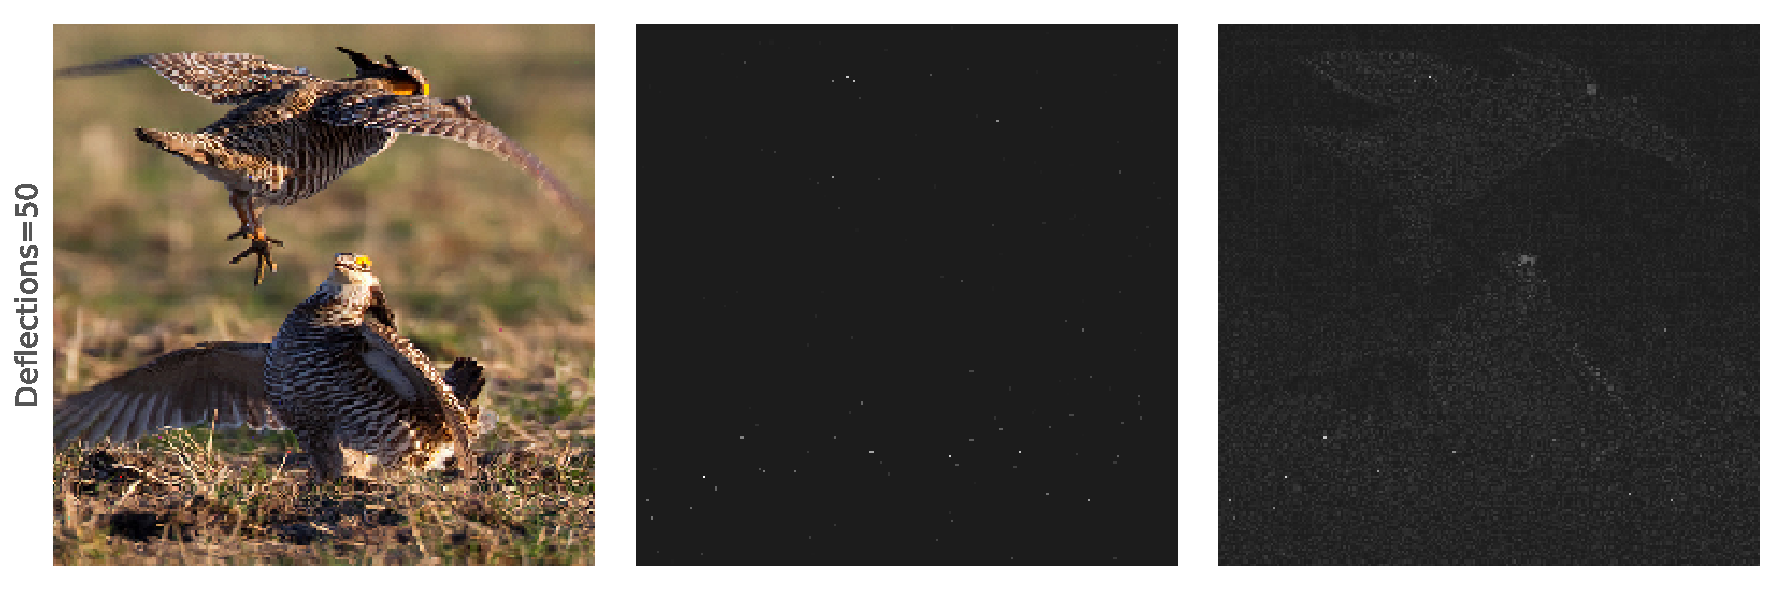
\includegraphics[width=1\linewidth, scale=0.9]{figures/pixel/image_corruption_x_50.pdf}
   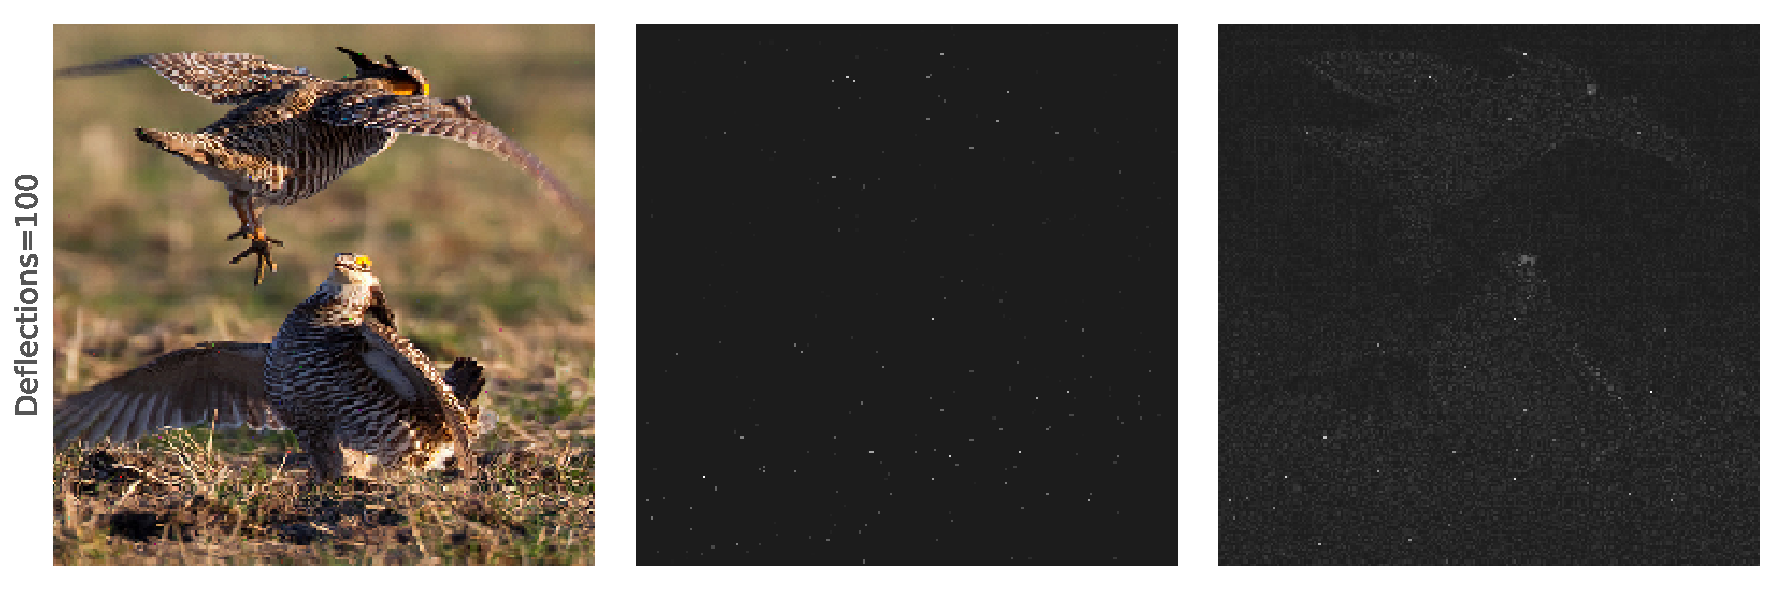
\includegraphics[width=1\linewidth, scale=0.9]{figures/pixel/image_corruption_x_100.pdf}
   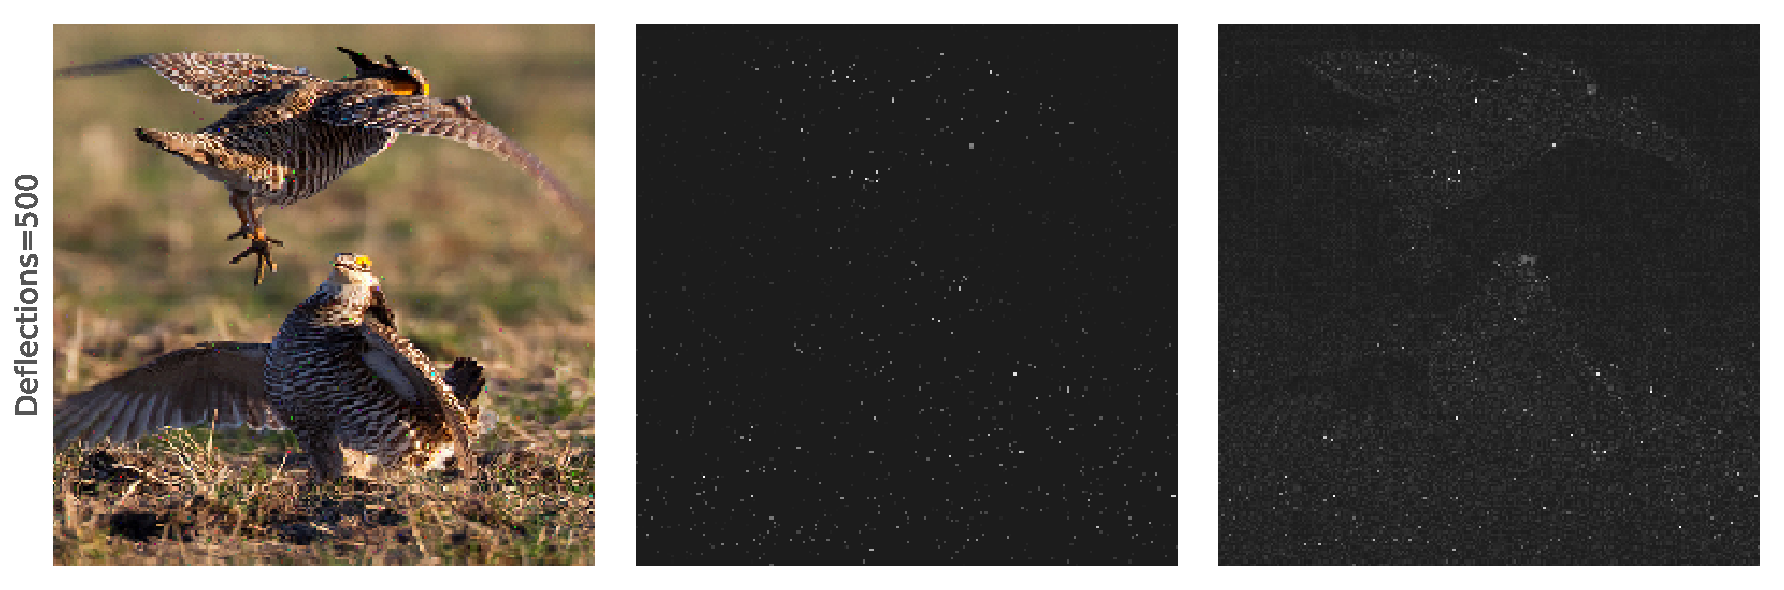
\includegraphics[width=1\linewidth, scale=0.9]{figures/pixel/image_corruption_x_500.pdf}
   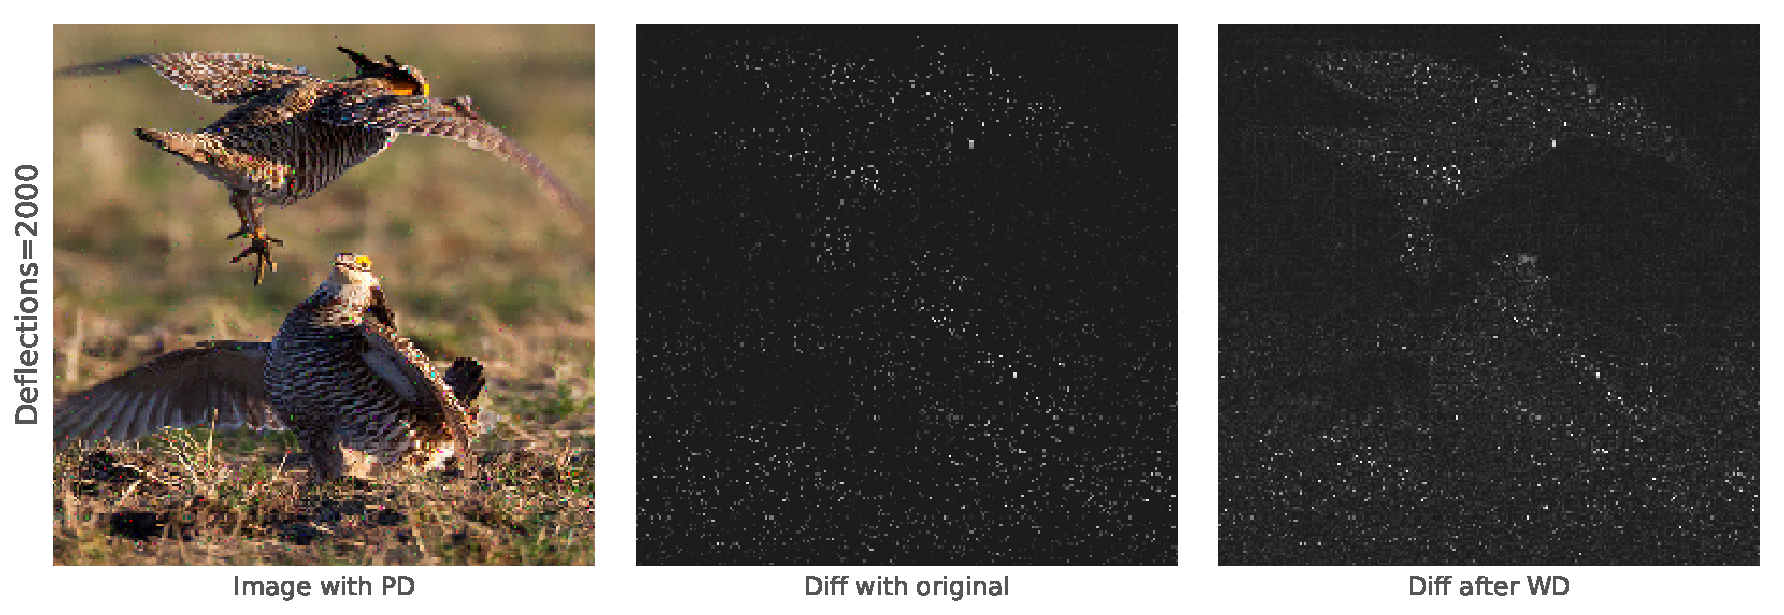
\includegraphics[width=1\linewidth, scale=0.9]{figures/pixel/image_corruption_x_2000.pdf}
   \label{fig:pixeldeflection}
   \caption[Impact Of Pixel Deflection]{Left: Image with given number of pixels deflected. Middle: Difference between clean image and deflected image. Right: Difference after denoising.}
   
\end{figure}

\begin{figure}[H]
   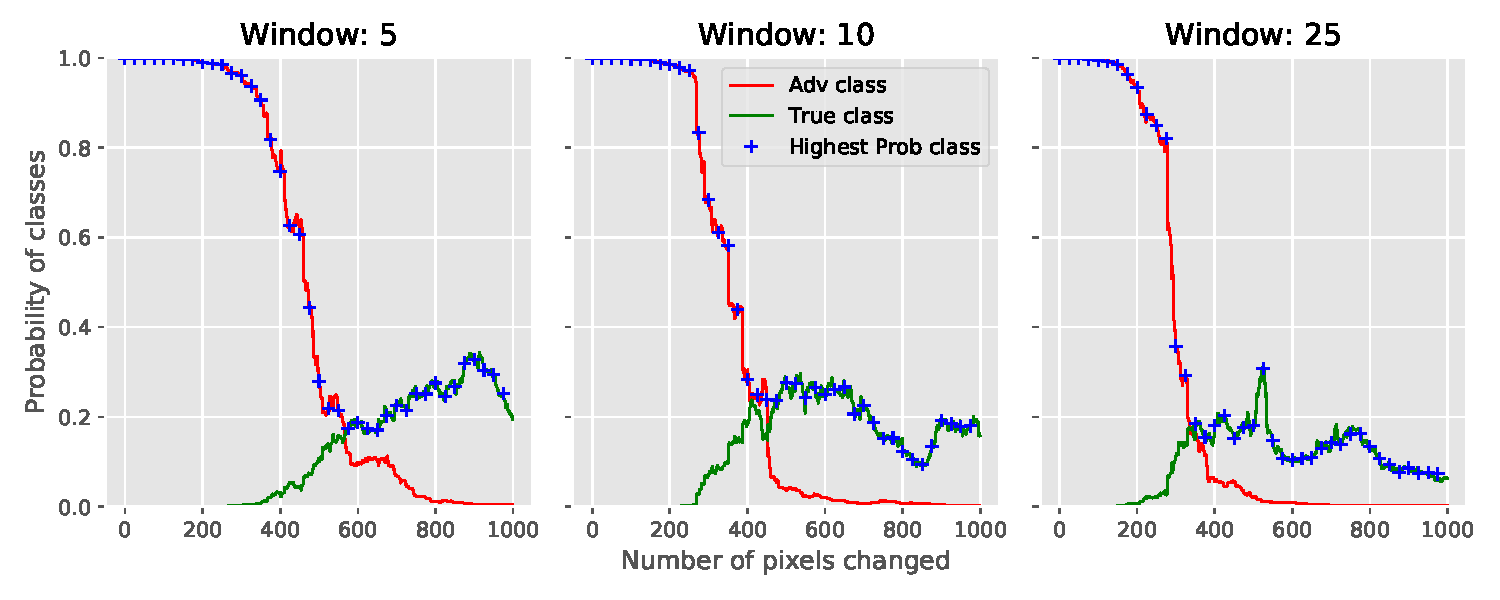
\includegraphics[width=1\linewidth]{figures/pixel/clean_pixel.pdf}
   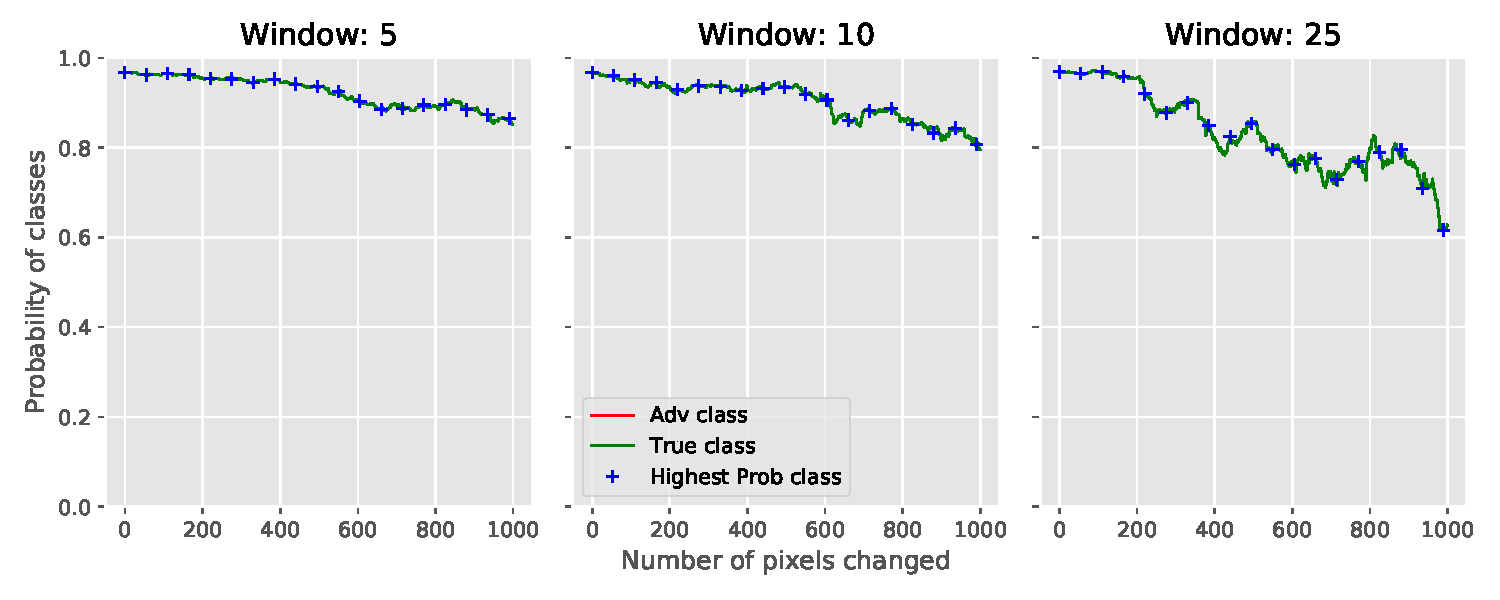
\includegraphics[width=1\linewidth]{figures/pixel/clean_pixel_no_adv.pdf}
   \caption[Impact on clean images]{Average classification probabilities for an adversarial image (top) and clean image (bottom) after pixel deflection (Image size: 299x299)}
   \label{fig:pixelloss}
\end{figure}


%We will briefly demonstrate that state-of-the-art classifiers are robust to this sort of pixel-level corruption.
%TODO: Maybe move this to the experiments section?
As shown in Figure ~\ref{fig:pixelloss}, even changing as much as $1\%$ (\ie $10$ times the amount changed in our experiments) of the original pixels does not alter the classification of a clean image.
However, application of pixel deflection enables the recovery of a significant portion of correct classifications.

\subsection{Distribution of Attacks}

Most attacks search the entire image plane for adversarial perturbations, without regard for the location of the image content.
%The attack models have no special preference for changing pixels which belong to the object in the image. 
This is in contrast with the classification models, which show high activation in regions where an object is present ~\cite{Yosinski2015UnderstandingNN,Chattopadhyay2017GradCAMGG}. %RYAN: might as well cite yourself here too!
This is especially true for attacks which aim to minimize the $L_p$ norm of their changes for large values of $p$, as this gives little to no constraint on the total number of pixels perturbed.
In fact, Lou \etal \cite{FoveationbasedMALuo2015} use the object coordinates to mask out the background region and show that this defends against some of the known attacks. 
 

\begin{figure}[H]
   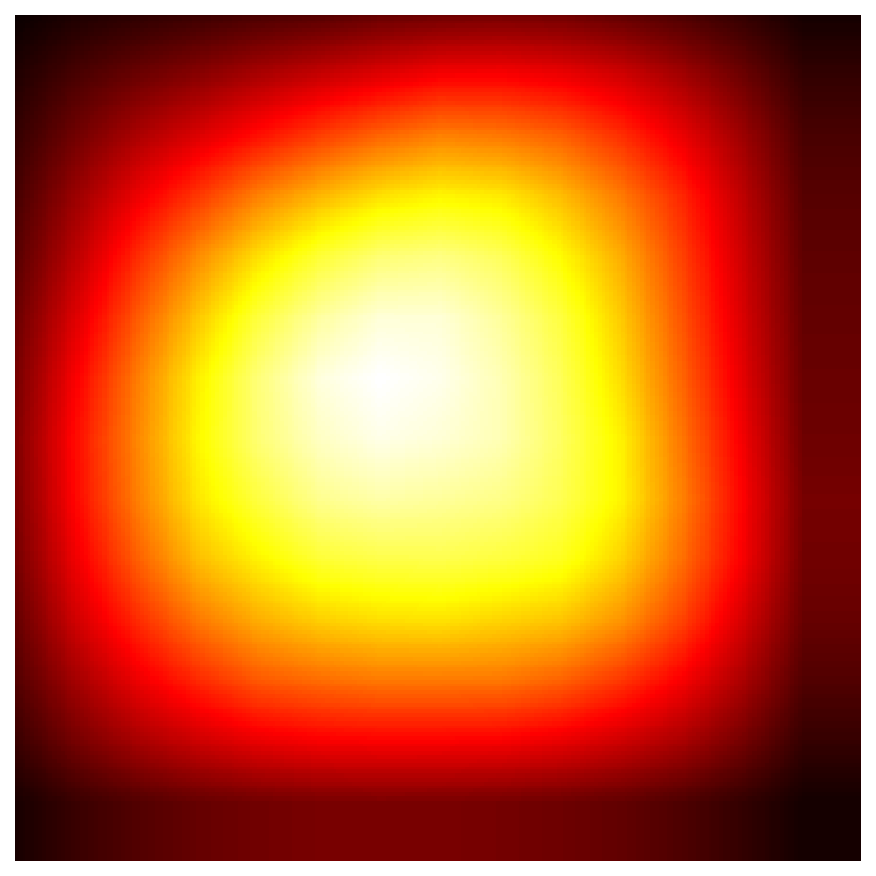
\includegraphics[width=0.242\linewidth]{figures/pixel/vis_attack_X.pdf}
   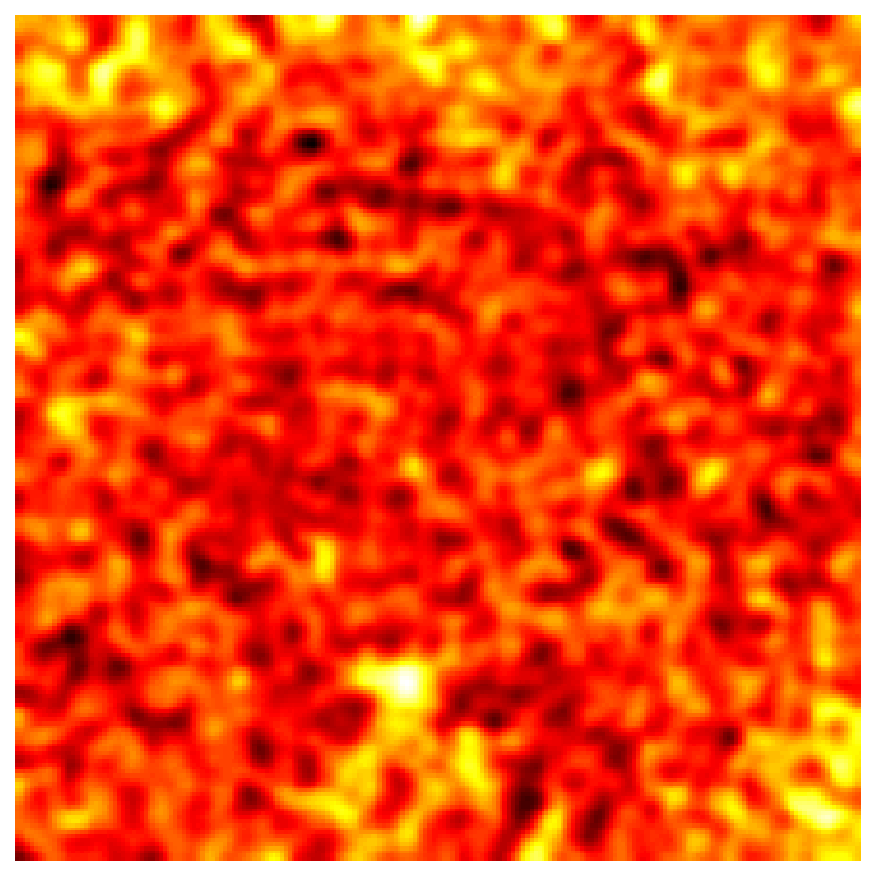
\includegraphics[width=0.242\linewidth]{figures/pixel/vis_attack_0.pdf}
   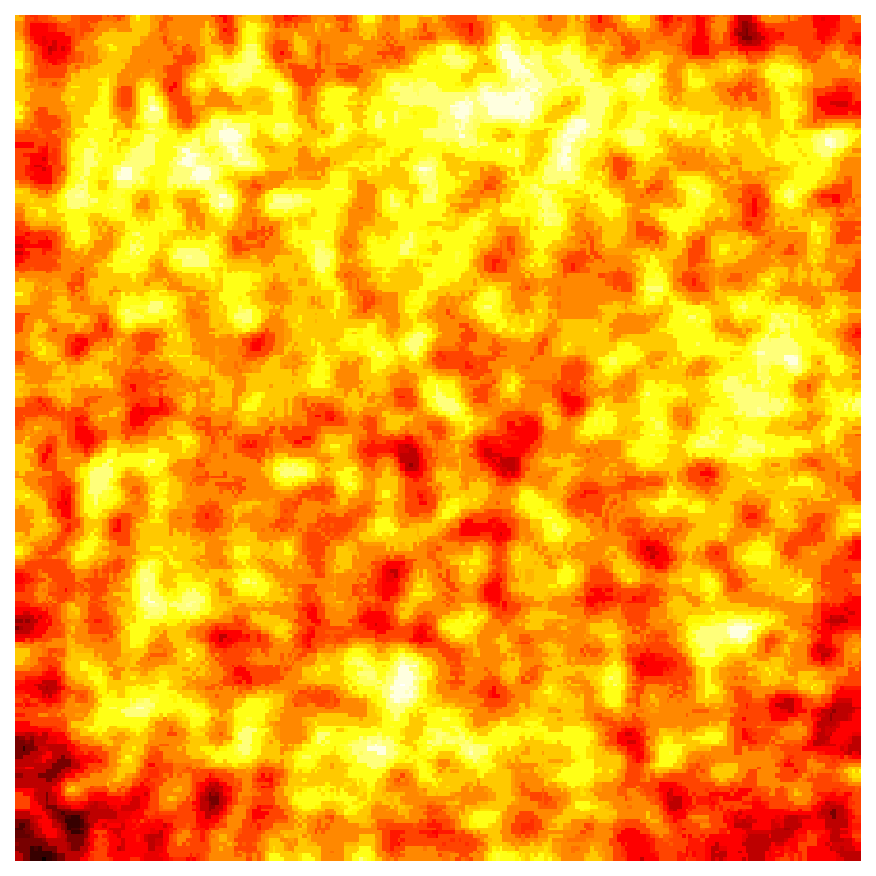
\includegraphics[width=0.242\linewidth]{figures/pixel/vis_attack_1.pdf}
   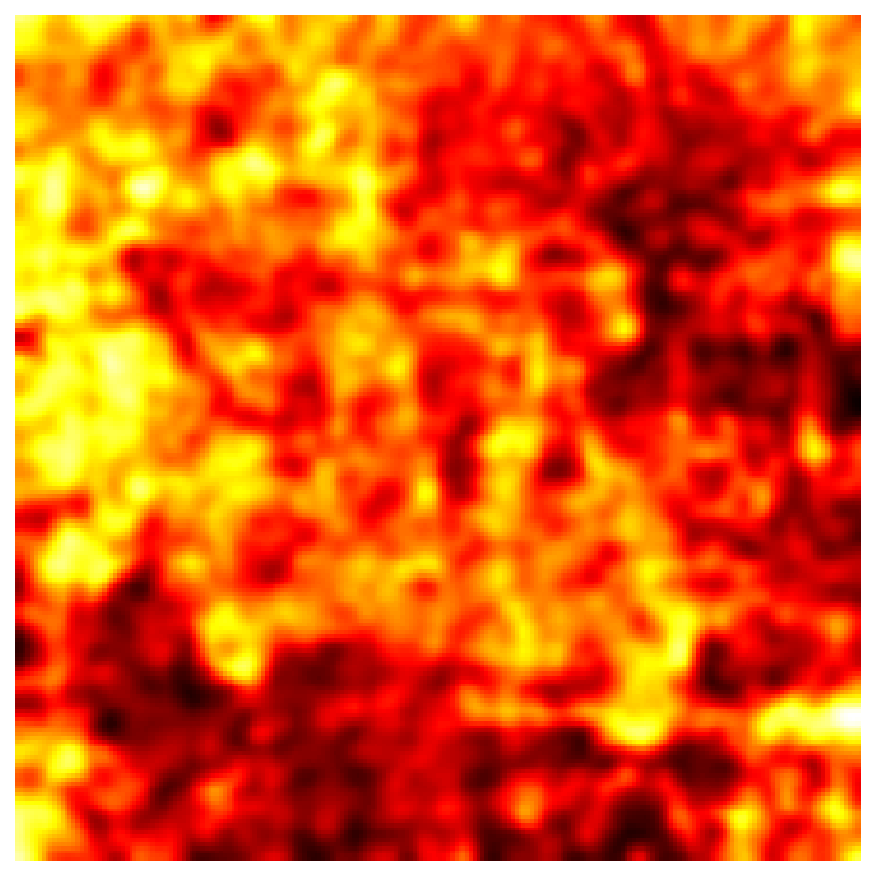
\includegraphics[width=0.242\linewidth]{figures/pixel/vis_attack_2.pdf}
   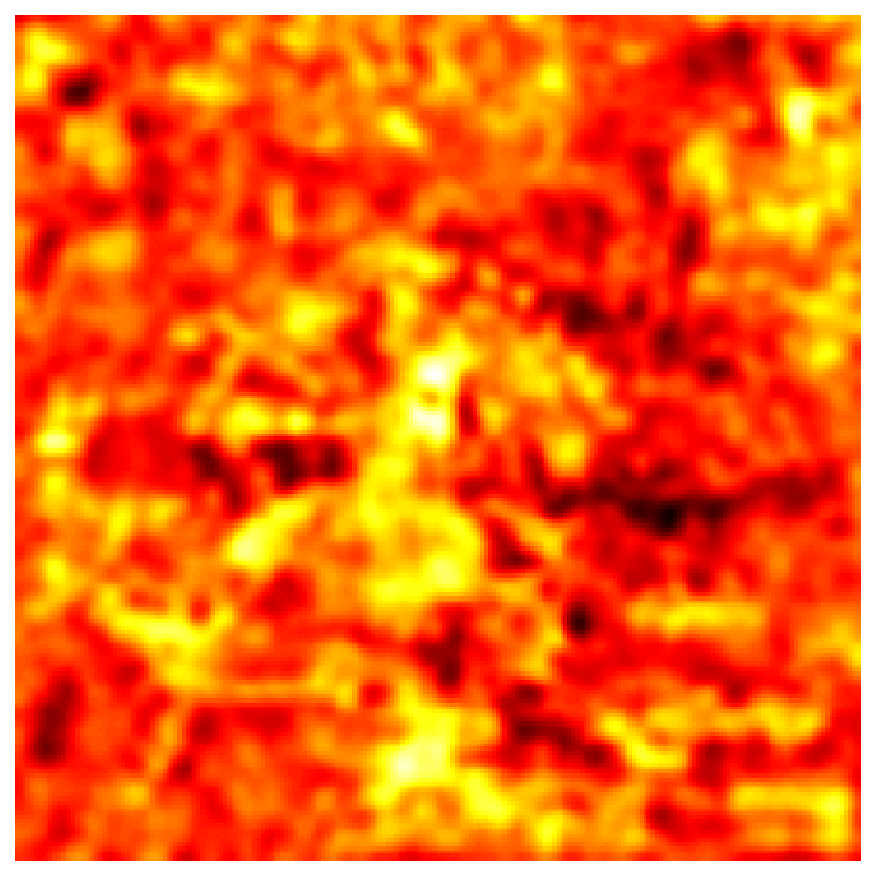
\includegraphics[width=0.242\linewidth]{figures/pixel/vis_attack_3.pdf}
   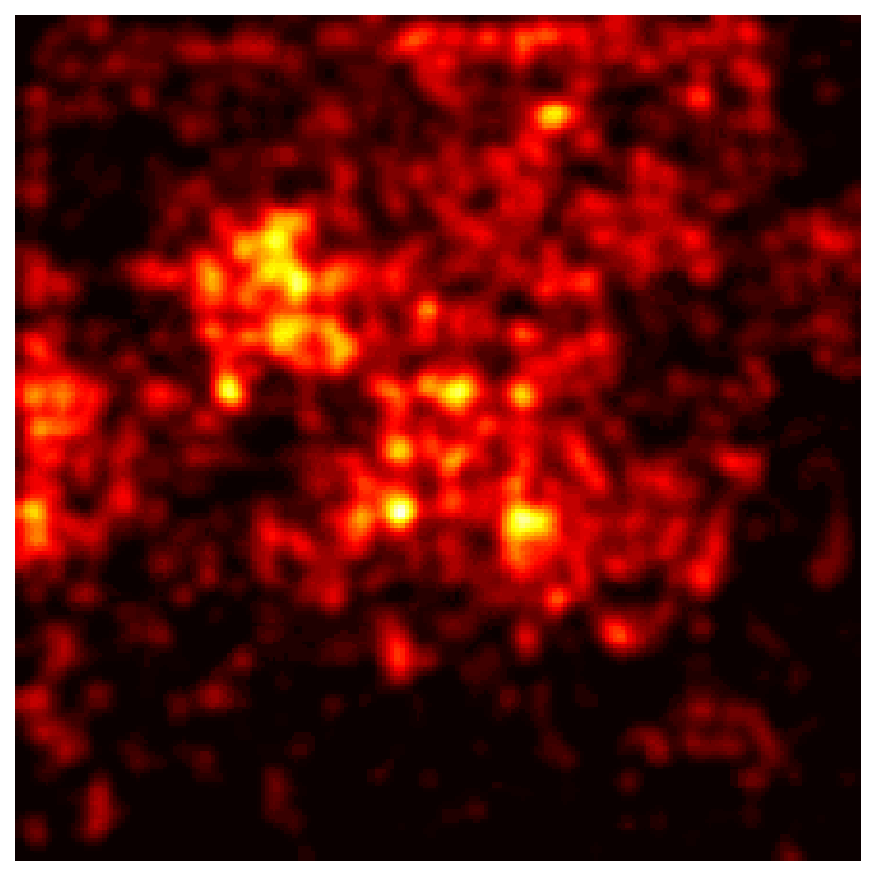
\includegraphics[width=0.242\linewidth]{figures/pixel/vis_attack_4.pdf}
   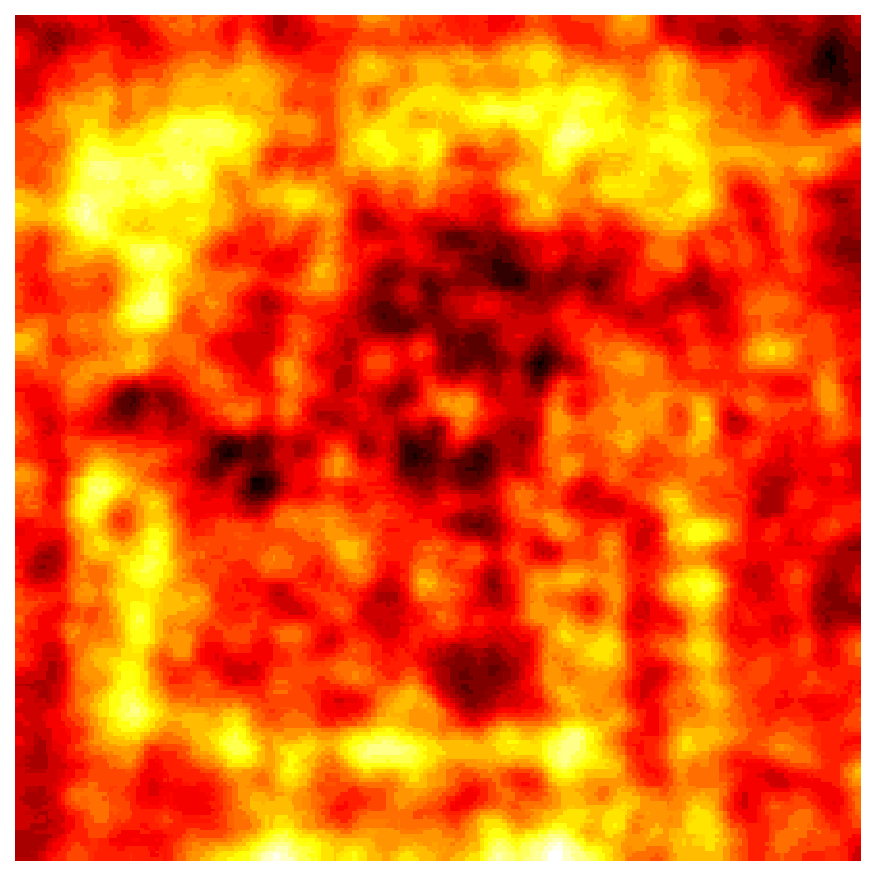
\includegraphics[width=0.242\linewidth]{figures/pixel/vis_attack_5.pdf}
   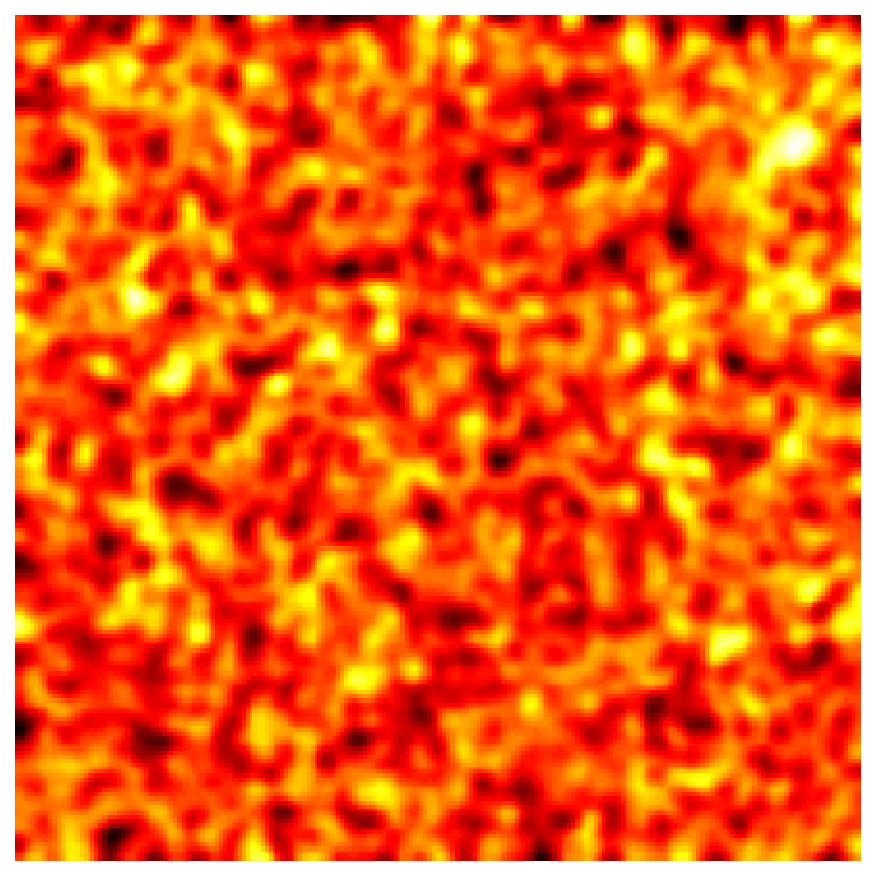
\includegraphics[width=0.242\linewidth]{figures/pixel/vis_attack_9.pdf}
   
   \caption[Location of perturbation]{Visualization showing average location in the image where perturbation is added by an attacker.
   Clockwise from top left:
   Localization of most salient object in the image, FGSM, IGSM, FGSM-2 (higher $\epsilon$), Deep Fool, JSMA, LBFGS and Carlini-Wagner attack.
   \label{fig:visattack}}
   
\end{figure}

In Figure ~\ref{fig:visattack} we show the average spatial distribution of perturbations for several attacks, as compared to the distribution of object locations (top left). 
%TODO:IMP
Based on these ideas, we explore the possibility of updating the pixels in the image such that the probability of that pixel being updated is inversely proportional to the likelihood of that pixel containing an object.


\section{Targeted Pixel Deflection \label{sec:tpd}}

As we have shown in section ~\ref{sec:pdrop}, image classification is robust against the loss of a certain number of pixels. 

% RYAN: "to do correspond to a relevant" is a grammar error. Not sure what it is trying to say.  Fixed ~Nick
In natural images, many pixels do not correspond to a relevant semantic object and are therefore not salient to classification.
%TODO:IMP use the ImageNet to calculate this ratio
Classifiers should then be more robust to pixel deflection if more pixels corresponding to the background are dropped as compared to the salient objects.
Luo \etal \cite{FoveationbasedMALuo2015} used this idea to mask the regions which did not contain the object,
%They use the ground truth co-ordinates from image localization dataset to obtain a mask.
however, their method has two limitations which we will seek to overcome.

First, it requires ground-truth object coordinates and it is, therefore, difficult to apply to unlabeled inputs at inference time. 
We solve this by using a variant of class activation maps to obtain an approximate localization for salient objects.
Class activation maps ~\cite{CAMZhou2016LearningDF}  are a weakly-supervised localization ~\cite{WeaklyOquab2015IsOL} technique in which
the last layer of a CNN, often a fully connected layer, is replaced with a global average pooling layer. 
This results in a heat map which lacks pixel-level precision but is able to approximately localize objects by their class.
%TODO: DONE I am not sure if the sentence above is grammatically correct. Please check and rephrase if necessary.
We prefer to use weakly supervised localization over saliency maps ~\cite{SALICONHuang2015}, as saliency maps are trained on human eye fixations 
and thus do not always capture object classes ~\cite{DeepGazeKmmerer2014DeepGI}. 
Other weakly supervised localization techniques, such as regions-of-interest ~\cite{Prakash2017SemanticPI}, capture more than a single object and thus are not suitable for improving single-class classification.

Second, completely masking out the background deteriorates classification of classes for which the model has come to rely on the co-occurrence of non-class objects.
For instance, airplanes are often accompanied by a sky-colored background, and most classifiers will have lower confidence when trying to classify an airplane outside of this context.
%RYAN: perhaps say "our approach can be interpreted as a Bayesian one, in which..."
We take a Bayesian approach to this problem and use stochastic re-sampling of the background. 
This preserves enough of the background to protect classification and drops enough pixels to weaken the impact of adversarial input. 


\subsection{Robust Activation Map \label{sec:robustmap}}

Class activation maps ~\cite{CAMZhou2016LearningDF} are a valuable tool for approximate semantic object localization.
%visualization tool to depict the likelihood of the presence of an object class for a given image.
Consider a convolutional network with $k$ output channels on the final convolution layer ($f$) with spatial dimensions of $x$ and $y$, and let $\boldsymbol{w}$ be a vector of size $k$ which is the result of applying a global max pool on each channel. 
This reduces channel to a single value, $\boldsymbol{w_k}$.
The class activation map, $M_c$ for a class $c$ is given by:
\begin{equation}
M_c(x,y) = \sum_k \boldsymbol{w}_k^c \; f_k(x,y)
\end{equation}
Generally, one is interested in the map for the class for which the model assigns the highest probability.
However, in the presence of adversarial perturbations to the input, the highest-probability class is likely to be incorrect.
Fortunately, our experiments show that an adversary which successfully changes the most likely class tends to leave the rest of the top-k classes unchanged.
Our experiments show that $38\%$ of the time the predicted class of adversarial images is the second highest class of the model for the clean image. 
Figure ~\ref{fig:untarget} shows how the class of adversarial image relates to predictions on clean images.
%TODO: numbers, tables anything to validate this
ImageNet has one thousand classes, many of which are fine-grained. 
Frequently, the second most likely class is a synonym or close relative of the main class (\eg ``Indian Elephant'' and ``African Elephant'').
To obtain a map which is robust to fluctuations of the most likely class, we take an exponentially weighted average of the maps of the top-$k$ classes. 
\begin{equation}
	\widehat{M}(x,y) = \sum_i^k \frac{M_{c_i}(x,y)}{2^i}
\end{equation}
%We will refer to this robust activation maps as $\widehat{M}(x,y)$. 
We normalize the map by diving it by its max so that values are in the range of $[0,1]$. %TODO: include this in the formula?
Even if the top-1 class is incorrect, this averaging reduces the impact of mis-localization of the object in the image. 
\begin{figure}[H]
   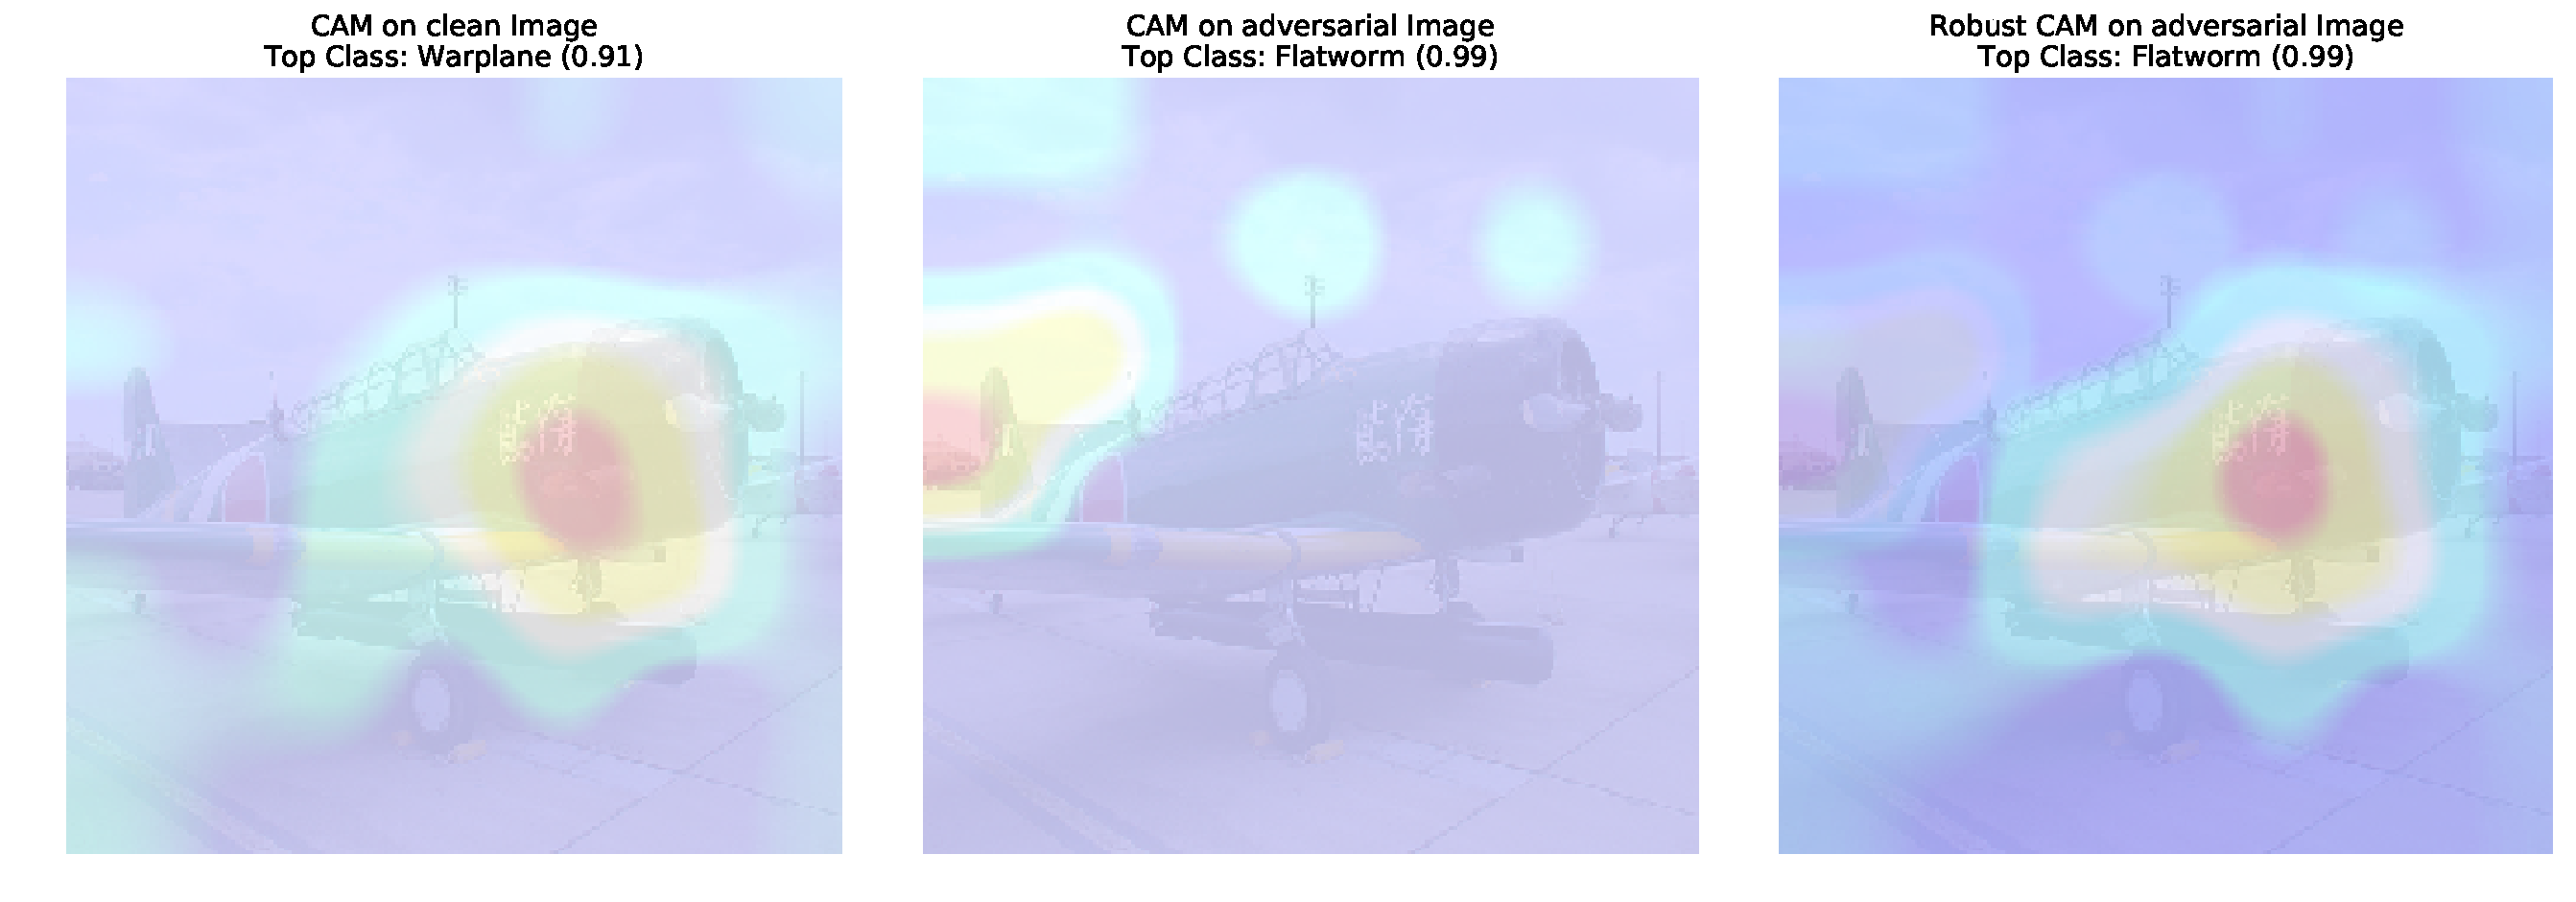
\includegraphics[width=1\linewidth]{figures/pixel/robust_cam.pdf}
   \caption[Robust Activation Maps]{Difference between standard activation maps and robust maps under the presence of an adversary.}
   \label{fig:robustcam}
\end{figure}

The appropriate number of classes $k$ to average over depends on the total number of classes.
For ImageNet-1000, we used a fixed $k=5$.
While each possible class has its own class activation map (CAM), only a single robust activation map is generated for a particular image, combining information about all classes.
ImageNet covers wide variety of object classes and most structures found in other datasets are represented in ImageNet even if class names are not bijectional.
Therefore, Robust Activation Map (R-CAM) is trained once on ImageNet but can also localize objects from Pascal-VOC or Traffic Signs. 


\section{Wavelet Denoising\label{sec:wavelet}}
Because both pixel deflection and adversarial attacks add noise to the image, it is desirable to apply a denoising transform to lessen these effects.
Since adversarial attacks do not take into account the frequency content of the perturbed image, they are likely to pull the input away from the class of likely natural images in a way which can be detected and corrected using a multi-resolution analysis. 

%RYAN: combined these cites into one, not sure if that's what was wanted
Works such as  ~\cite{BayesShrinkChang2000,Simoncelli1999BayesianDO,field1987relations} have shown that natural images exhibit regularities in their wavelet responses which can be learned from data and used to denoise images.
These regularities can also be exploited to achieve better lossy image compression, the basis of JPEG2000.
Many vision and neuroscience researchers  ~\cite{Marcelja1980MathematicalDO,Rust2005SpatiotemporalEO,Hubel1959ReceptiveFO} have suggested that the visual systems of many animals take advantage of these priors, as the simple cells in the primary visual cortex have been shown to have Gabor-like receptive fields.

Swapping pixels within a window will tend to add noise with unlikely frequency content to the image, particularly if the window is large.
% RYAN: I would remove this dicussion of JPEG, unless you plan to cite your DCC paper, that starts HERE------------
This kind of noise can be removed by image compression techniques like JPEG, however, the quantization process in JPEG uses fixed tables that are agnostic to image content, and it quantizes responses at all amplitudes while the important image features generally correspond to large frequency responses.
This quantization reduces noise but also gets rid of some of the signal. % (This can be observed as reduced PSNR of JPEG image as compared to original image).

Therefore, it is unsurprising that JPEG compression recovers correct classification on some of the adversarial images but  also reduces the classification accuracy on clean images \cite{Kurakin2016AdversarialEI,Das2017KeepingTB,Dziugaite2016ASO,CounteringAIGuo17}. 
Dziugaite \etal \cite{Dziugaite2016ASO} reported loss of $8$\% accuracy on clean images after undergoing JPEG compression. 
%TODO, if we decide to cite our current DCC paper, maybe we can cite that here. We provide more clear answer on that.
%We attribute the success of JPEG against adversarial images to the nonuniform quantization of spatially localized DCT block coefficients, reflecting similar assumptions about the local frequency content of natural images to wavelet denoising.

We, therefore, seek filters with frequency response better suited to joint space-frequency analysis than the DCT blocks (and more closely matching representations in the early ventral stream, so that features which have a small filter response are less perceptible) and quantization techniques more suited to denoising. %TODO: DONE reword
%RYAN: AND ENDS HERE --------------------
%RYAN: ... then describe why the wavelet is good independent of JPEG. If not, I think you need to show that JPEG is effective.
Wavelet denoising uses wavelet coefficients obtained using \textit{Discrete Wavelet Transform} \cite{DWTantonini1992image}.
The wavelet transform represents the signal as a linear combination of orthonormal wavelets.
These wavelets form a basis for the space of images and are separated in space, orientation, and scale.
%TODO maybe specify DWT for discrete wavelet transform and use that after that first time?
The Discrete Wavelet Transform is widely used in image compression ~\cite{JPEG2000Adams2001} and image denoising ~\cite{BayesShrinkChang2000,WaveletDenoisingRangarajan2002,Simoncelli1999BayesianDO}.

%It has benefits over Discrete Cosine Transform as it tries to recover signal regardless of the frequency content. %TODO what does this mean?
While the noise introduced by dropping a pixel is mostly high-frequency, the same cannot be said about the adversarial perturbations.
Several attempts have been made to quantify distribution of adversarial perturbations \cite{DropoutFeinman2017,ForesightLin2017DetectingAA} but recent work by Carlini and Wagner \cite{EasilyDetectedCarlini2017} has shown that most techniques fail to detect adversarial examples.
We have observed that for the perturbations added by well-known attacks, wavelet denoising yields superior results as compared to block DCT. %TODO maybe just say JPEG
%TODO compare DCT/shrinkage to show benefit of wavelet, SOLOMON: add intuition

\subsection{Hard \& Soft Thresholding}
%The Wavelet Transform alone is a linear and a lossless process. 
%Therefore, the noise reduction happens only if we threshold the wavelet coefficients.
%Most compression techniques use hard-thresholding, in which values below a threshold are set to zero.
%Jansen \etal \cite{ThresholdingJansen2012noise} observed that hard-thresholding of wavelets introduces other forms of noise %in the output, and soft-thresholding maintains better PSNR.
%Thus, we use soft-thresholding for the purposes of our experiment.

%Let the Discrete Wavelet Transform and its inverse be represented as $\mathcal{T}$ and $\mathcal{T}^{-1}$. 
%We will represent the transformation of image $X$ using $\mathcal{T}$ as $\hat{X}$.   
%If $Q$ be the thresholding function with $T_h$ as the threshold.
%Then the hard-threshold is obtained by $Q(\hat{X}) = \hat{X} \; \forall \; |\hat{X}| > T_h$ and soft-thresholding is computed as $Q(\hat{X}) = \text{sign}(\hat{X})\times \text{max}(0,|\hat{X}| - T_h) $.
%Soft-threshold is able to shrink the values below the $T_h$ which avoids the noise introduced by hard threshold.

%NEW
The process of performing a wavelet transform and its inverse is lossless and thus does not provide any noise reduction.
In order to reduce adversarial noise, we need to apply thresholding to the wavelet coefficients before inverting the transform.
Most compression techniques use a hard thresholding process, in which all coefficients with magnitude below the threshold are set to zero: $Q(\hat{X}) = \hat{X} \; \forall \; |\hat{X}| > T_h$, where $\hat{X}$ is the wavelet transform of $X$, and $T_h$ is the threshold value.
The alternative is soft thresholding, in which we additionally subtract the threshold from the magnitude of coefficients above the threshold: $Q(\hat{X}) = \text{sign}(\hat{X})\times \text{max}(0,|\hat{X}| - T_h)$.
Jansen \etal \cite{ThresholdingJansen2012noise} observed that hard thresholding results in over-blurring of the input image, while soft thresholding maintains better PSNR.
By reducing all coefficients, rather than just those below the threshold, soft thresholding avoids introducing extraneous noise.
This allows our method to preserve classification accuracy on non-adversarial images.
%NEW


\subsection{Adaptive Thresholding \label{sec:contentthresholding}}
% TODO: Is content-aware confusing term? I had adaptive but that undersells what we do. 
Determining the proper threshold is very important, and the efficacy of our method relies on the ability to pick a threshold in an adaptive, image specific manner.
The standard technique for determining the threshold for wavelet denoising is to use a universal threshold formula called \textit{VisuShrink}. 
For an image $X$ with $N$ pixels, this is given by $\sigma\sqrt{2\log N}$, where $\sigma$ is the variance of the noise to be removed and is a hyper-parameter. 
However, we used \textit{BayesShrink} \cite{BayesShrinkChang2000}, which models the threshold for each wavelet coefficient as a Generalized Gaussian Distribution (GGD). 
The optimal threshold is then assumed to be the value which minimizes the expected mean square error \ie
\begin{equation}
T_h*(\sigma_x, \beta) = \argmin_{T_h} E(\hat{X} - X)^2 \; \approx \frac{\sigma^2}{\sigma_x}
\label{eqn:bayesshrink}
\end{equation}
where $\sigma_x$ and $\beta$ are parameters of the GGD for each wavelet sub-band.
In practice, an approximation, as shown on right side of equation ~\ref{eqn:bayesshrink}, is used. 
This ratio, also called $T_{\text{Bayes}}$, adapts to the amount of noise in the given image.
Within a certain range of $\beta$ values, BayesShrink has been shown to effectively remove artificial noise while preserving the perceptual features of natural images ~\cite{BayesShrinkChang2000,WaveletDenoisingRangarajan2002}.
As our experiments are carried out with images from ImageNet, which is a collection of natural images, we believe this is an appropriate thresholding technique to use.
% RYAN: this next paragraph might fit better with the experiments section
Yet another popular thresholding technique is Stein's Unbiased Risk Estimator (SUREShrink), which computes unbiased estimate of $E(\hat{X} - X)^2 $. SUREShrink requires optimization to learn $T_h$ for a given coefficient. We empirically evaluated results and SUREShrink did not perform as well as BayesShrink. Comparative results are  shown in Table ~\ref{tblshrink}.

\section{Method}

The first step of our method is to corrupt the adversarial noise by applying targeted pixel deflection as follows: %RYAN this method really seems more like it is part of your algorithm. Maybe you need a section about combining pixel deflection with the adaptive denoising.

(a) Generate a robust activation map $\widehat{M}$, as described in section ~\ref{sec:robustmap}.

(b) Uniformly sample a pixel location $(x,y)$ from the image, and obtain the normalized activation map value for that location, $v_{x,y} = \widehat{M}(x,y)$.

(c) Sample a random value from a uniform distribution $\mathcal{U}(0,1)$. If $v_{x,y}$ is lower than the random value, we deflect the pixel using the algorithm shown in Algorithm  ~\ref{alg:swap}. 

(d) Iterate this process $K$ times. \\

The following steps are used to soften the impact of pixel deflection:

(a) Convert the image to $YC_bC_r$ space to decorrelate the channels. $YC_bC_r$ space is perceptually meaningful and thus has similar denoising advantages to the wavelets.  

(b) Project the image into the wavelet domain using the discrete wavelet transform. We use the \textit{db1} wavelet, but similar results were obtained with \textit{db2} and \textit{haar} wavelets. 

(c) Soft threshold the wavelets using BayesShrink. 

(d) Compute the inverse wavelet transform on the shrunken wavelet coefficients.

(e) Convert the image back to RGB.

\section{Experimental Design\label{sec:exp}}

We tested our method on $1000$ randomly selected images from the ImageNet ~\cite{Deng2009ImageNetAL} Validation set. 
We use ResNet-50 ~\cite{he2015deep} as our classifier. 
We obtain the pre-trained weights from TensorFlow's GitHub repository.
These models achieved a Top-1 accuracy of $76\%$ on our selected images. %TODO:IMP REMOVE THIS????????
This is in agreement with the accuracy numbers reported in ~\cite{he2015deep} for a single-model single-crop inference.

By the definition set by adversarial attacks, an attack is considered successful by default if the original image is already mis-classified. 
In this case, the adversary simply returns the original image unmodified. 
However, these cases are not useful for measuring the effectiveness of an attack or a defense as there is no pixel level difference between the images.
As such, we restrict our experiments to those images which are correctly classified in the absence of adversarial noise.
Our attack models are based on the Cleverhans  ~\cite{papernot2017cleverhans} library\footnote{https://github.com/tensorflow/cleverhans} with model parameters that aim to achieve the highest possible misclassification score with a normalized RMSE ($|\bm{L}_2|$) budget of $0.02-0.04$.

We will publicly release  our implementation code.
%Impact of adversary can only be detected when there is a diff
%We reject the images from our set which yields incorrect classification on the clean image. 

\subsection{Training}

%Unlike models that train a new network  ~\cite{Tramr2017TheSO,Meng2017MagNetAT} our model has very few hyper-parameters.
Our defense model has three hyper-parameters, which is significantly fewer than the classification models it seeks to protect, making it preferable over defenses which require retraining of the classifier such as  ~\cite{Tramr2017TheSO,Meng2017MagNetAT}.
These three hyper-parameters are: $\sigma$, a coefficient for \textit{BayesShrink}, $r$, the window size for pixel deflection, and $K$, the number of pixel deflections to perform.
Using a reduced set of $300$ images from ImageNet Validation set, We perform a linear search over a small range of these hyper-parameters. 
%We use $300$ images from ImageNet Validation set to search for optimal hyper-parameters. 
These images are not part of the set used to show the results of our model.
A particular set of hyper-parameters may be optimal for one attack model, but not for another.  
This is primarily because attacks seek to minimize different $L_p$ norms, and therefore generate different types of noise.
%Different values of these parameters perform best on different attack strategies. 
%Primarily because attacks are minimizing different $L_p$ norms. 
To demonstrate the robustness of our defense, we select a single setting of the hyper-parameters to be used against all attack models.
Figure ~\ref{fig:hyperparam} shows a visual indication of the variations in performance of each model across various hyper-parameter settings. 
In general, as the $K$ and $r$ increase, the variance of the resulting classification accuracy increases.  
This is primarily due to the stochastic nature of pixel deflection - as more deflections are performed over a wider window, a greater variety of transformed images can result.
%Variance in the accuracy increases with the increase in window size and number of iterations, this is due to stochastic nature of pixel deflection.

\begin{figure}[H]
   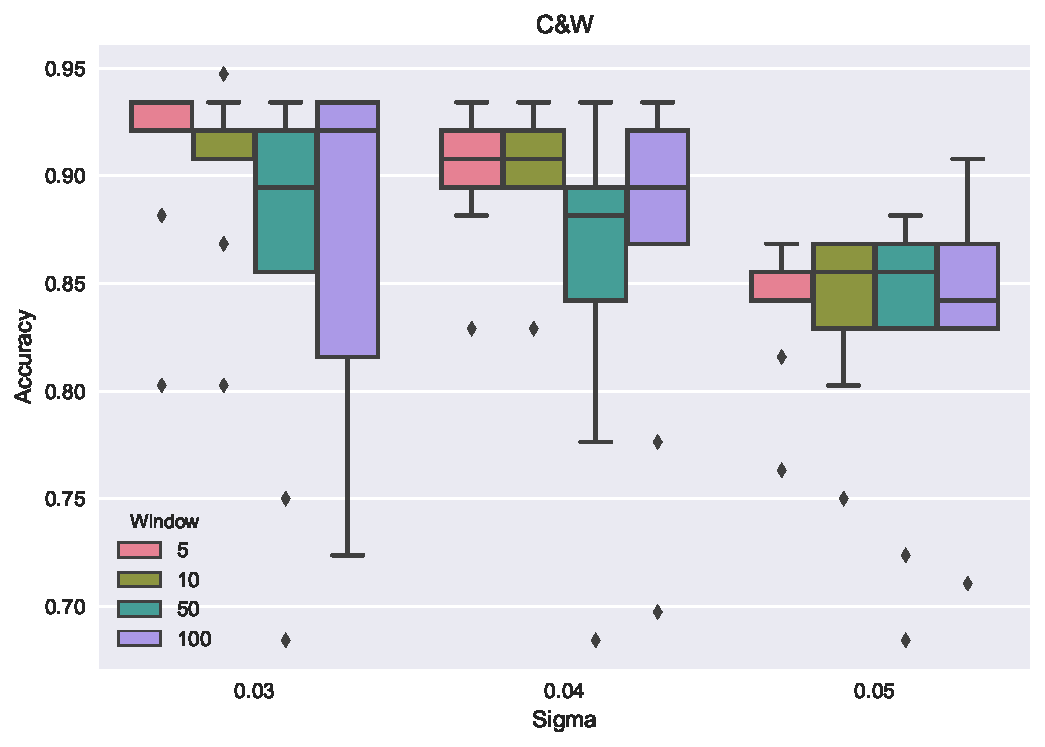
\includegraphics[width=0.49\linewidth]{figures/pixel/CW.pdf}
   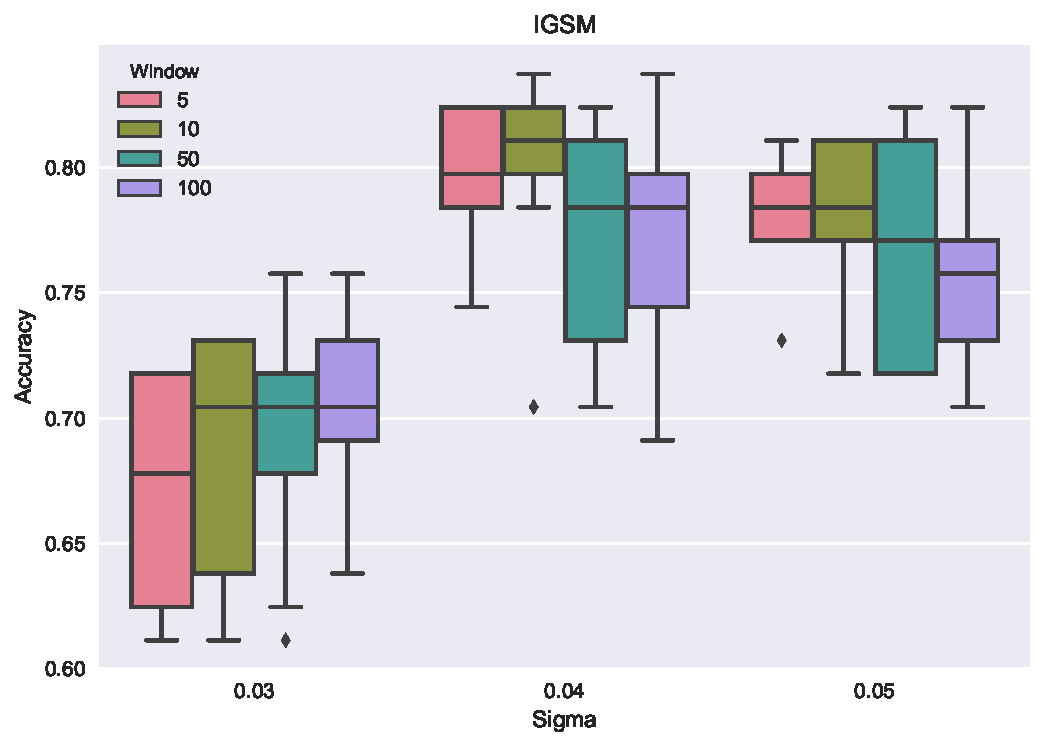
\includegraphics[width=0.49\linewidth]{figures/pixel/IGSM.pdf}
   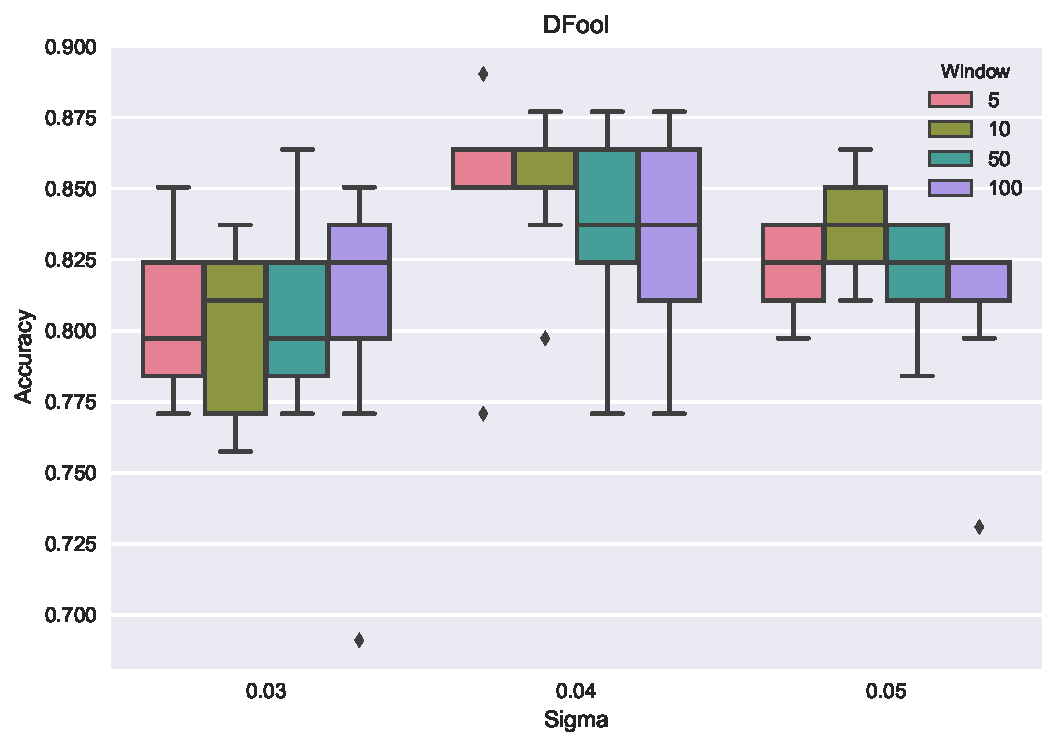
\includegraphics[width=0.49\linewidth]{figures/pixel/DFool.pdf}
   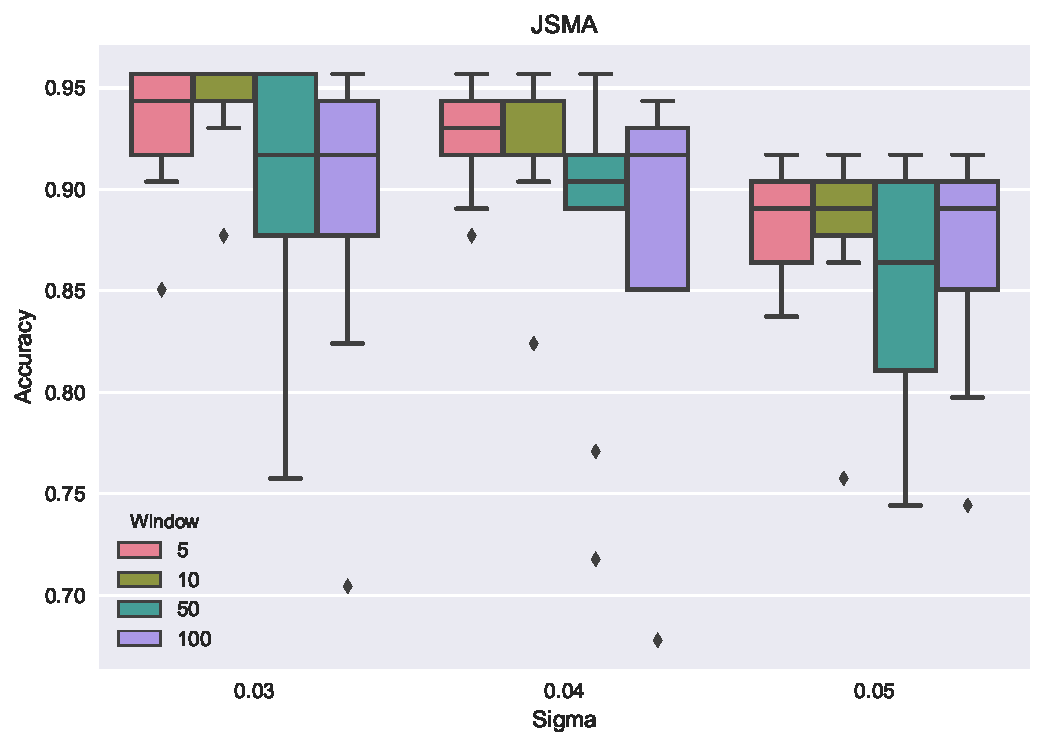
\includegraphics[width=0.49\linewidth]{figures/pixel/JSMA.pdf}
   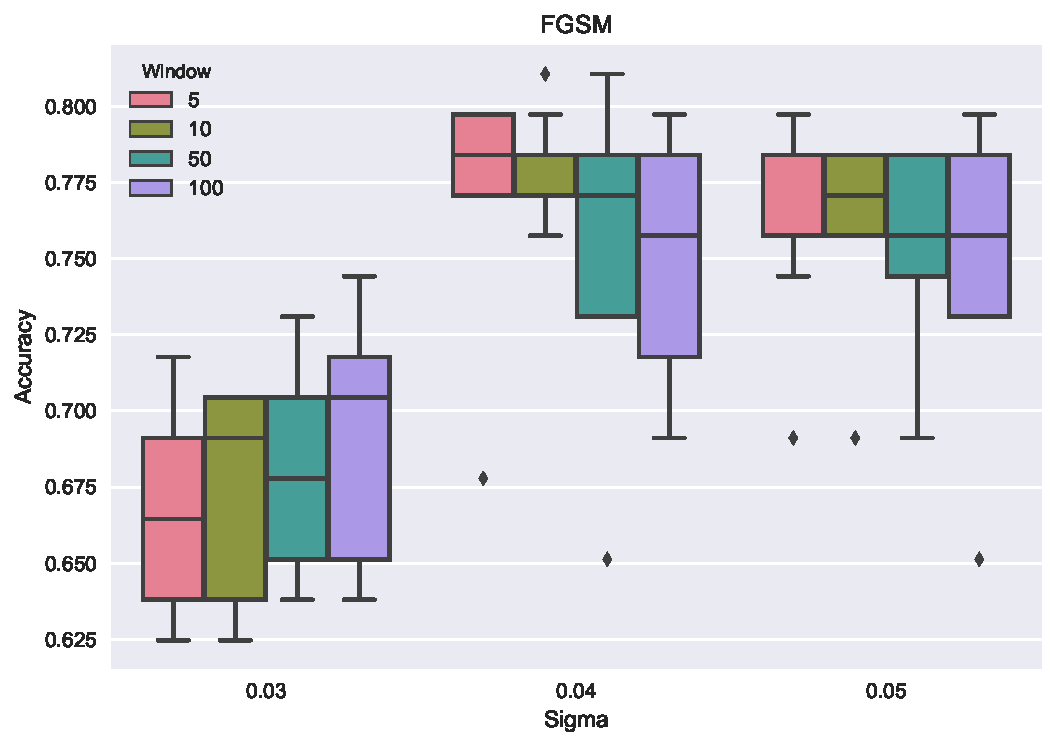
\includegraphics[width=0.49\linewidth]{figures/pixel/FGSM.pdf}
   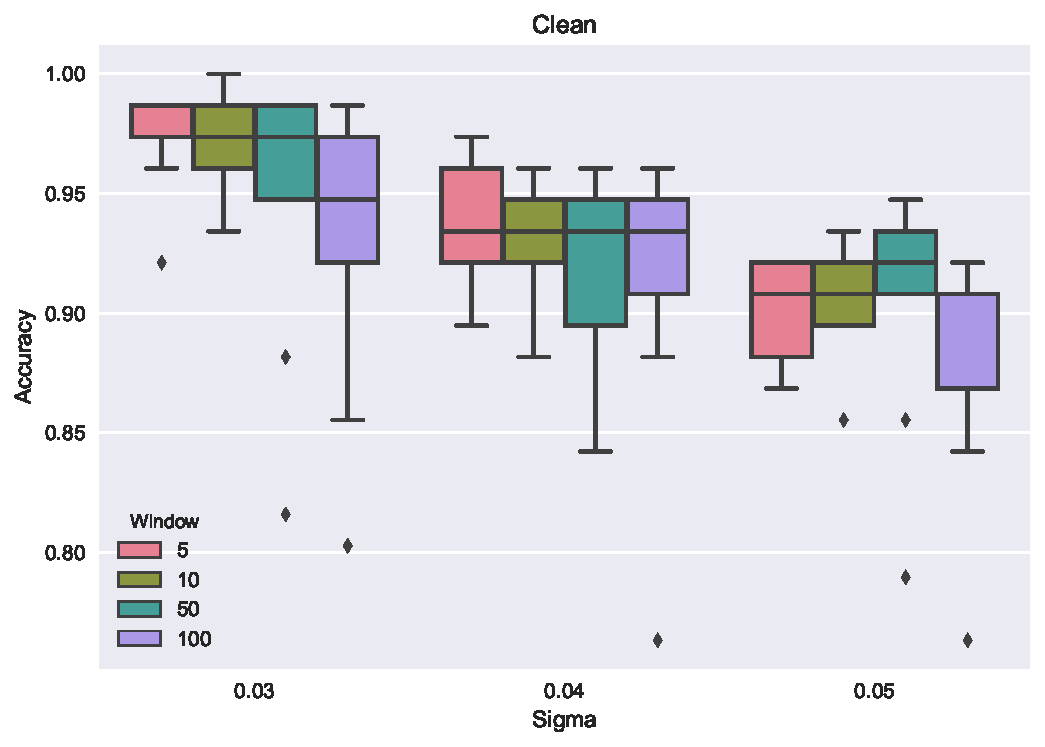
\includegraphics[width=0.49\linewidth]{figures/pixel/Clean.pdf}
   \caption[Parameter Search]{Linear search for model parameters}
   \label{fig:hyperparam}
\end{figure}

\section{Results \& Discussion \label{sec:results_pixel}}

\begin{table}[H]
\centering
\rowcolors{1}{White}{Gray}
\begin{tabular}{lcccc}
\textbf{Model} & \multicolumn{1}{l}{$|\boldsymbol{L}_2|$} & \multicolumn{1}{l}{\textbf{No Defense}} & \multicolumn{2}{l}{\textbf{With Defense}} \\ \hline
 & \multicolumn{1}{l}{} & \multicolumn{1}{l}{} & Single & Ens-10 \\ \cline{4-5} 
 \textbf{Clean} & 0.00 & 100 & 98.3 & \textbf{98.9} \\ \hline
\textbf{FGSM} & 0.05 & 20.0 & 79.9 & \textbf{81.5} \\
\textbf{IGSM} & 0.03 & 14.1 & 83.7 & \textbf{83.7} \\
\textbf{DFool} & 0.02 & 26.3 & 86.3 & \textbf{90.3} \\
\textbf{JSMA} & 0.02 & 25.5 & 91.5 & \textbf{97.0} \\
\textbf{LBFGS} & 0.02 & 12.1 & 88.0 & \textbf{91.6} \\
\textbf{C\&W} & 0.04 & 04.8 & 92.7 & \textbf{98.0}
\\
 \multicolumn{5}{c}{Large perturbations} \\ \hline
 &&&&\\
\textbf{FGSM} & 0.12 & 11.1 & 61.5 &  \textbf{70.4}\\
\textbf{IGSM} & 0.09 & 11.1 & 62.5 &  \textbf{72.5}\\
\textbf{DFool} & 0.08 & 08.0 & 82.4 &  \textbf{88.9}\\
\textbf{JSMA} & 0.05 & 22.1 & 88.9 &  \textbf{92.1}\\
\textbf{LBFGS} & 0.04 & 12.1 & 77.0 & \textbf{89.0} \\
\end{tabular}
\caption[Classification Accuracy with Pixel Deflection]{ Params: $\sigma=0.04$, Window=10, Deflections=100 \\Top-1 accuracy on applying pixel deflection and wavelet denoising across various attack models. We evaluate non-efficient attacks at larger $|\bm{L}_P|$ which leave visible perturbations to show the robustness of our model.
 \label{tblresults}}
\end{table}
In Table ~\ref{tblresults} we present results obtained by applying our transformation against various untargeted white-box attacks. 
Our method is agnostic to classifier architecture, and thus shows similar results across various classifiers. 
For brevity, we report only results on ResNet-50. 
Results for other classifiers are provided in Table ~\ref{tblmodels}.
The accuracy on clean images without any defense is 100\% because we didn't test our defense on images which were misclassified before any attack.
We do not report results for targeted attacks as they are harder to generate ~\cite{Carlini2017TowardsET} and easier to defend. 
Due to the stochastic nature of our model, we benefit from taking the majority prediction over ten runs; this is reported in Table ~\ref{tblresults} as Ens-10.
%The benefits of doing majority ensemble are particularly pronounced against attacks such as JSMA which are based on activation intensity, thus different set of deflected pixels combine to weaken the adversary.

%\subsection{Results on larger samples}
We randomly sampled 10K images from ILSVRC2012 validation set; this contained all 1000 classes with minimum of $3$ images per class.

%\vspace{-2mm}
\begin{table}[H]
%\vspace{-1mm}
\centering
\rowcolors{1}{White}{Gray}
%\setlength{\tabcolsep}{0.6em}
\begin{tabular}{lcccc}
\textbf{Attack} & \multicolumn{1}{l}{$|\boldsymbol{L}_2|$} & \multicolumn{1}{l}{\textbf{No Defense}} & \multicolumn{2}{l}{\textbf{With Defense}} \\ \hline
 \multicolumn{3}{l}{Window=10, Deflections=100}  & Single & Ens-10 \\ \hline 
\small{Clean} & 0.00 & 100 & 98.1 & \textbf{98.9} \\ 
\small{FGSM} & 0.04 & 19.2 & 79.7 & \textbf{81.2} \\
\small{IGSM} & 0.03 & 11.8 & 81.7 & \textbf{82.4} \\
\small{DFool} & 0.02 & 18.0 & 87.7 & \textbf{92.4} \\
\small{JSMA} & 0.02 & 24.9 & 93.0 & \textbf{98.1} \\
\small{LBFGS} & 0.02 & 11.6 & 90.3 & \textbf{93.6} \\
\small{C\&W} & 0.04 & 05.2 & 93.1 & \textbf{98.3}   \\ \hline
\end{tabular}
%\vspace{-3mm}
\caption[Accuracy Under Various Attacks]{Top-1 accuracy of our model on various attack models.}
%\vspace{-2mm}
\end{table}

\subsection{Results on various classifiers}
Original classification accuracy of each classifier on selected $1000$ images is reported in the table.
However, we omit the images that were originally incorrectly classified, thus the accuracy of clean images without defense is always $100\%$.
Weights for each classifier were obtained from Tensorflow GitHub repository
\footnote{https://github.com/tensorflow/models/tree/master/research/slim\#Pretrained}. \\

\begin{table}[H]
\centering
\rowcolors{1}{White}{Gray}
\begin{tabular}{lcccc}
\textbf{Model} & \multicolumn{1}{l}{$|\boldsymbol{L}_2|$} & \multicolumn{1}{l}{\textbf{No Defense}} & \multicolumn{2}{l}{\textbf{With Defense}} \\ \hline
 & \multicolumn{1}{l}{} & \multicolumn{1}{l}{} & Single & Ens-10 \\ \cline{4-5} 
 \multicolumn{5}{c}{ResNet-50, original classification $76\%$} \\ \hline

\textbf{Clean} & 0.00 & 100 & 98.3 & \textbf{98.9} \\ \hline
\textbf{FGSM} & 0.05 & 20.0 & 79.9 & \textbf{81.5} \\
\textbf{IGSM} & 0.03 & 14.1 & 83.7 & \textbf{83.7} \\
\textbf{DFool} & 0.02 & 26.3 & 86.3 & \textbf{90.3} \\
\textbf{JSMA} & 0.02 & 25.5 & 91.5 & \textbf{97.0} \\
\textbf{LBFGS} & 0.02 & 12.1 & 88.0 & \textbf{91.6} \\
\textbf{C\&W} & 0.04 & 04.8 & 92.7 & \textbf{98.0} \\
\end{tabular}
\caption[ResNet-50 under Pixel Deflection]{Top-1 accuracy of ResNet-50 with pixel deflection on various attack models. 
 \label{tblmodels}}
\end{table}
 
 
 
 
 
\begin{table}[H]
\centering
\rowcolors{1}{White}{Gray}
\begin{tabular}{lcccc}
\textbf{Model} & \multicolumn{1}{l}{$|\boldsymbol{L}_2|$} & \multicolumn{1}{l}{\textbf{No Defense}} & \multicolumn{2}{l}{\textbf{With Defense}} \\ \hline
 & \multicolumn{1}{l}{} & \multicolumn{1}{l}{} & Single & Ens-10 \\ \cline{4-5} 
 \multicolumn{5}{c}{VGG-19, original classification $71\%$} \\ \hline

\textbf{Clean} & 0.00 & 100 & 99.8 & \textbf{99.8} \\ \hline
\textbf{FGSM} & 0.05 & 12.2 & 79.3 & \textbf{81.3} \\
\textbf{IGSM} & 0.04 & 9.79 & 79.2 & \textbf{81.6} \\
\textbf{DFool} & 0.01 & 23.7 & 83.9 & \textbf{91.6} \\
\textbf{JSMA} & 0.01 & 29.1 & 95.8 & \textbf{98.5} \\
\textbf{LBFGS} & 0.03 & 13.8 & 83.0 & \textbf{93.9} \\
\textbf{C\&W} & 0.04 & 0.00 & 93.1 & \textbf{97.6} \\
\end{tabular}
\caption[VGG-19 under Pixel Deflection]{Top-1 accuracy of VGG-19 with pixel deflection on various attack models. 
 \label{tblmodels1}}
\end{table}
 
 
 \begin{table}[H]
\centering
\rowcolors{1}{White}{Gray}
\begin{tabular}{lcccc}
\textbf{Model} & \multicolumn{1}{l}{$|\boldsymbol{L}_2|$} & \multicolumn{1}{l}{\textbf{No Defense}} & \multicolumn{2}{l}{\textbf{With Defense}} \\ \hline
 & \multicolumn{1}{l}{} & \multicolumn{1}{l}{} & Single & Ens-10 \\ \cline{4-5} 
 \multicolumn{5}{c}{Inception-v3, original classification $78\%$} \\ \hline

\textbf{Clean} & 0.00 & 100 & 98.1 & \textbf{98.5} \\ \hline
\textbf{FGSM} & 0.05 & 22.1 & 85.8 & \textbf{87.1} \\
\textbf{IGSM} & 0.04 & 15.5 & \textbf{89.7} & 89.1 \\
\textbf{DFool} & 0.02 & 27.2 & 82.6 & \textbf{85.3} \\
\textbf{JSMA} & 0.02 & 24.2 & 93.7 & \textbf{98.6} \\
\textbf{LBFGS} & 0.02 & 12.5 & 87.1 & \textbf{91.0} \\
\textbf{C\&W} & 0.04 & 07.1 & 93.9 & \textbf{98.5} \\
\end{tabular}
\caption[Inception-v3 under Pixel Deflection]{Top-1 accuracy of Inception-v3 with pixel deflection on various attack models. 
 \label{tblmodels2}}
\end{table}

\subsection{Comparison of results} - 
There are two main challenges when seeking to compare defense models. 
First, many attack and defense techniques primarily work on smaller images, such as those from CIFAR and MNIST.
The few proposed transformation based defense techniques which work on larger-scale images are extremely recent, and currently under review ~\cite{MitigatingAnon208,CounteringAIGuo17}.
Second, because different authors target both different $|\bm{L}_P|$ norms and different perturbation magnitudes, it is difficult to balance the strength of various attacks.
We achieved $98\%$ recovery on C\&W with $|\bm{L}_2|$ of 0.04 on ResNet-50, where Xie \etal ~\cite{MitigatingAnon208} reports $97.1\%$ on ResNet-101 and $98.8\%$ on ens-adv-Inception-ResNet-v2.
ResNet-101 is as stronger classifier than ResNet-50 and ens-adv-Inception-Resnet-v2 ~\cite{Tramr2017EnsembleAT} is an ensemble of classifiers specifically trained with adversarial augmentation. 
They do not report the $|\bm{L}_2|$ norm of the adversarial perturbations, and predictions are made on an ensemble of 21 crops.
Guo \etal ~\cite{CounteringAIGuo17} have reported (normalized) accuracy of $92.1\%$ on C\&W with $|\bm{L}_2|$ of 0.06, and their predictions are on an ensemble of 10 crops.

To present a fair comparison across various defenses we only measure the fraction of images which are no longer misclassified after the transformation.  
This ratio is known as  Destruction Rate and was originally proposed in [24]. 
Value of $1$ means all the misclassified images due to the adversary are correctly classified after the transformation.

\begin{table}[H]
\centering
\rowcolors{1}{White}{Gray}
\setlength{\tabcolsep}{0.4em}
%\vspace{-2mm}
\begin{tabular}{lllll}
\textbf{Defense}              & \textbf{FGSM}  & \textbf{IGSM}  & \textbf{DFool} & \textbf{C\&W}  \\ \hline
\multicolumn{5}{c}{Feature Squeezing (Xu et al \cite{FeatureSqueezingXu2017})}                                                \\ \hline
\small{(a) Bit Depth (2 bit)} & 0.132          & 0.511          & 0.286          & 0.170          \\
\small{(b) Bit Depth (5 bit)} & 0.057          & 0.022          & 0.310          & 0.957          \\
\small{(c) Median Smoothing (2x2)} & 0.358          & 0.422          & 0.714          & 0.894          \\
\small{(d) Median Smoothing (3x3)} & 0.264          & 0.444          & 0.500          & 0.723          \\
\small{(e) Non-local Mean (11-3-2)} & 0.113          & 0.156          & 0.357          & 0.936          \\
\small{(f) Non-local Mean (13-3-4)} & 0.226          & 0.444          & 0.548          & 0.936          \\
\small{Best model (b) + (c) + (f)} & 0.434          & 0.644          & 0.786          & 0.915          \\ \hline
\multicolumn{5}{c}{Random resizing + padding (Xie \etal \cite{MitigatingAnon208} )}                               \\ \hline
\small{Pixel padding}    & 0.050          & -              & 0.972          & 0.698          \\
\small{Pixel resizing}    & 0.360          & -              & 0.974          &    0.971       \\
\small{Padding + Resizing}   & 0.478          & -              & \textbf{0.983} & 0.969          \\ \hline
\multicolumn{5}{c}{Quilting + TVM (Guo \etal \cite{CounteringAIGuo17} )}                                         \\ \hline
\small{Quilting}        & 0.611          & 0.862          & 0.858          & 0.843          \\
\small{TVM + Quilting}& 0.619          & 0.866          & 0.866          & 0.841          \\
\small{Cropping + TVM + Quilting} & 0.629          & 0.882          & 0.883          & 0.859          \\ \hline
\multicolumn{5}{c}{Our work: PD - Pixel Deflection, R-CAM: Robust CAM}                                                                    \\ \hline
\small{PD}  & 0.735          & 0.880          & 0.914          & 0.931          \\
\small{PD + R-CAM}       & 0.746          & 0.912          & 0.911          & 0.952          \\
\small{PD + R-CAM + DCT}       & 0.737          & 0.906          & 0.874         & 0.930          \\
\small{PD + R-CAM + DWT}  & \textbf{0.769} & \textbf{0.927} & 0.948          & \textbf{0.981} \\ \hline
\end{tabular}
%\vspace{-3mm}
\caption[Destruction Rate]{Destruction Rate of various defense techniques. $|L_2|$ lies between $0.02 - 0.06$ and classifier accuracy is $76\%$.
We only include the Black-box attacks, where the attack model is not aware of the defense techniques. Single Pattern Attack and Ensemble pattern attack as reported in Xie et al \cite{MitigatingAnon208} are not reported.}
\end{table}

\begin{figure}[H]
\centering
   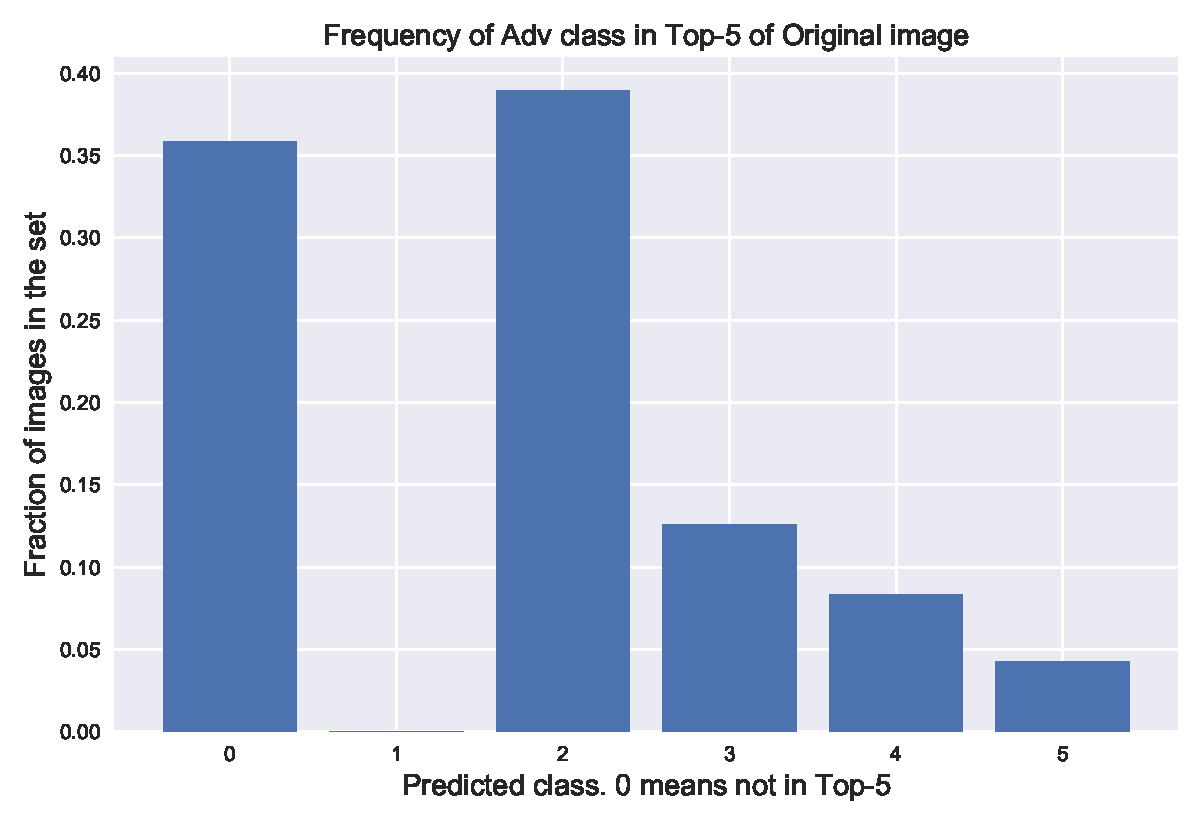
\includegraphics[width=0.49\linewidth]{figures/pixel/untargeted.pdf}
   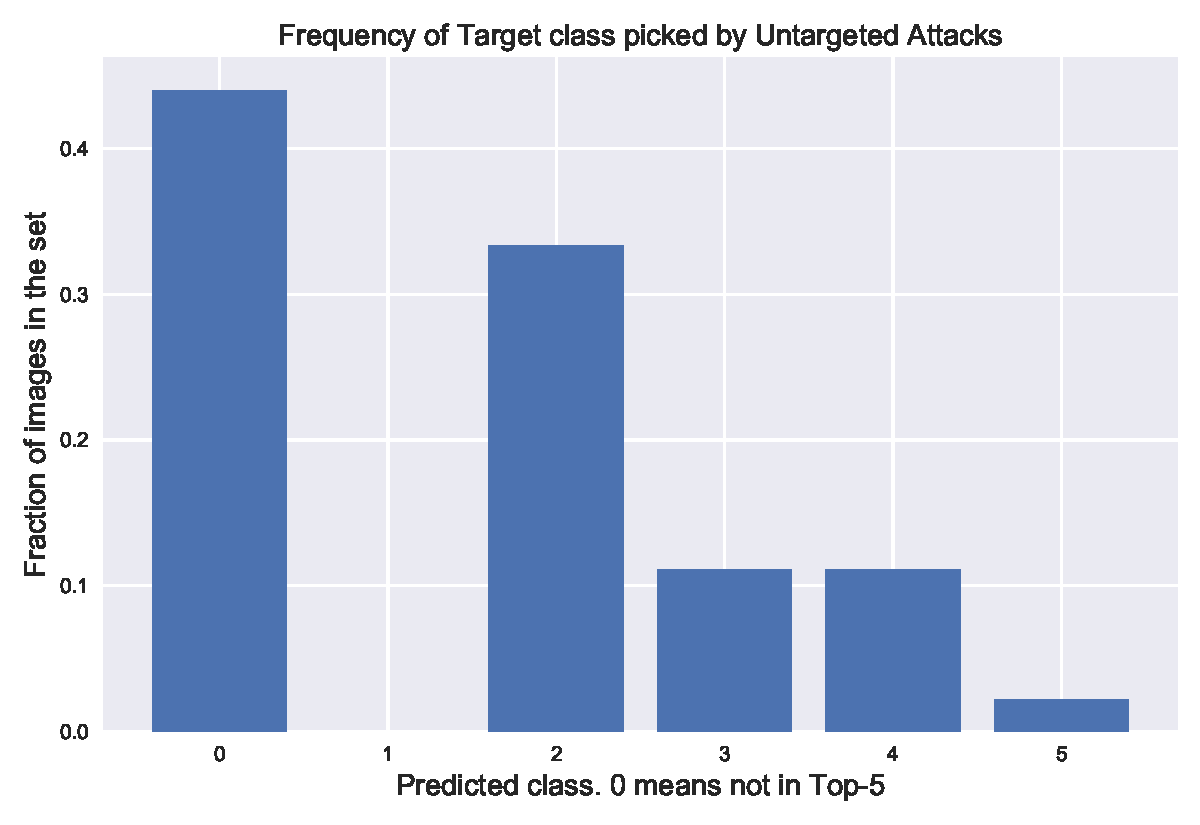
\includegraphics[width=0.49\linewidth]{figures/pixel/retargeted.pdf}
   \caption[Overlap of Classes under Adversary]{Left: Rank of adversarial class within the top-5 predictions for original images.  Right: Rank of original class within the top-5 predictions for adversarial images.  In both cases, 0 means the class was not in the top-5.}
   \label{fig:untarget}
\end{figure}
%We do not report Top-5 accuracy for these evaluations as reported by Kurakin\etal ~\cite{Kurakin2016AdversarialEI}, as the adversary often targets the second most likely class, leaving top-5 accuracy unaffected.
%In $64\%$ of the cases the mis-classified class was still within Top-5 picks barring the most likely class. 
As seen in Figure ~\ref{fig:untarget}, the predicted class of the perturbed image is very frequently among the classifier's top-5 predictions for the original image.
In fact, nearly $40\%$ of the time, the adversarial class was the second most-probable class of the original image.
Similarly, the original classification will often remain in the top-5 predictions for the adversarial image.
Unlike Kurakin \etal ~\cite{Kurakin2016AdversarialEI}, our results are in terms of top-1 accuracy, as this matches the objective of the attacker.
While top-1 accuracy is a more lenient metric for an attack method (due to the availability of nearly-synonymous alternatives to most classes in ImageNet-1000), it is a more difficult metric for a defense, as we must exactly recover the correct classification.
These facts render top-5 accuracy an unsuitable metric for measuring the efficacy of a defense.
%While evaluating an adversarial system this might be considered as a weaker result, however for a defense model this is a harder task, as the semantic difference in the classes between clean image and adversarial image is very low.
When evaluating stochastic transformations, it is quite common to use an ensemble of predictions to get a more generalized version of the model's performance.
We perform pixel deflection on a given image ten times and do a majority vote of the predicted classes to report the accuracy numbers. 
Results reported for Carlini \& Wagner ~\cite{Carlini2017TowardsET} attacks are only for $L_2$ loss, even though they can be applied for $L_0$ and $L_\infty$. 
Carlini \& Wagner attack has been shown to be effective with MNIST and CIFAR but their efficacy against large images is limited due to expensive computation. 



\subsection{Ablation studies}

Previous work ~\cite{Kurakin2016AdversarialEI,Dziugaite2016ASO} has demonstrated the efficacy of JPEG compression as a defense against adversarial attacks due to its denoising properties.
Das \etal ~\cite{Das2017KeepingTB} demonstrate that increasing the severity of JPEG compression defeats a larger percentage of attacks, but at the cost of accuracy on clean image.
As our method employs a conceptually similar method to reduce adversarial noise via thresholding in a wavelet domain, we use JPEG as a baseline for comparison.
%JPEG can also be considered as a method to reduce image noise. 
%Therefore, it is no surprise that JPEG has been shown to recover some of the attacks ~\cite{Kurakin2016AdversarialEI,Dziugaite2016ASO}.
%
%Thus we consider JPEG as control to demonstrate efficacy of wavelet denoising.
In Table ~\ref{tblimpact}, we report accuracy with and without wavelet denoising with soft thresholding.
While JPEG alone is effective against only a few attacks, the combination of JPEG and pixel deflection performs better than pixel deflection alone.
The best results are obtained from pixel deflection and wavelet denoising.
Adding JPEG on top of these leads to a drop in performance. 
\begin{table}[H]
\centering
\rowcolors{1}{White}{Gray}
\begin{tabular}{lllllll}
\textbf{Model} & \textbf{JPG} & \textbf{WD} & \textbf{PD} & \textbf{\begin{tabular}[c]{@{}l@{}}\,PD\\ JPG\end{tabular}} & \textbf{\begin{tabular}[c]{@{}l@{}}WD\\ \,PD\\ JPG\end{tabular}} & \textbf{\begin{tabular}[c]{@{}l@{}}WD\\ \,PD\end{tabular}} \\ \hline
\textbf{Clean} &  96.1 &  98.7 &  97.4 &      96.1 &           96.1 &     \textbf{98.9} \\
\textbf{FGSM} &  49.1 &  40.6 &  79.7 &      81.1 &           78.8 &     \textbf{81.5} \\
\textbf{IGSM} &  49.1 &  31.2 &  82.4 &      82.4 &           79.7 &     \textbf{83.7} \\
\textbf{DFool} &  67.8 &  61.1 &  86.3 &      86.3 &           86.3 &     \textbf{90.3} \\
\textbf{JSMA} &  91.6 &  89.1 &  95.7 &      93.0 &           93.0 &     \textbf{97.0} \\
\textbf{LBFGS} &  71.8 &  67.2 &  90.3 &      89.1 &           88.9 &     \textbf{91.6} \\
\textbf{C\&W} &  85.5 &  95.4 &  95.4 &      94.1 &           93.4 &     \textbf{98.0} \\
\end{tabular}
\caption[Comparison with JPEG]{ Params: $\sigma=0.04$, Window=10, Deflections=100 \\
Ablation study of pixel deflection (PD) in combination with wavelet denoising (WD) and JPEG compression.\label{tblimpact}}
\end{table}

\begin{table}[H]
\centering
\rowcolors{1}{White}{Gray}
\begin{tabular}{lrrrr}
\textbf{Model} & \multicolumn{1}{c}{\textbf{\begin{tabular}[c]{@{}c@{}}Hard\end{tabular}}} &  \multicolumn{1}{c}{\textbf{\begin{tabular}[c]{@{}c@{}}VISU\end{tabular}}} & \multicolumn{1}{c}{\textbf{\begin{tabular}[c]{@{}c@{}}SURE\end{tabular}}} & \multicolumn{1}{c}{\textbf{\begin{tabular}[c]{@{}c@{}}Bayes\end{tabular}}} \\ \hline
 \textbf{Clean} &               39.5 &        96.1 &        92.1 &         \textbf{98.9} \\
  \textbf{FGSM} &               35.9 &        63.8 &        79.7 &         \textbf{81.5} \\
  \textbf{IGSM} &               42.5 &        67.8 &        81.1 &         \textbf{83.7} \\
 \textbf{DFool} &               37.2 &        78.4 &        87.7 &         \textbf{90.3} \\
 \textbf{JSMA} &               39.9 &        93.0 &        93.0 &         \textbf{97.0} \\
  \textbf{LBFGS} &               37.2 &        81.1 &        90.4 &         \textbf{91.6} \\
   \textbf{C\&W} &               36.8 &        93.4 &        92.8 &         \textbf{98.0} \\
\end{tabular}
\caption[Comparsion of Thresholding]{ Params: $\sigma=0.04$, Window=10, Deflections=100 \\
Comparison of various thresholding techniques, after application of pixel deflection. \label{tblshrink}}
\end{table}

In Table ~\ref{tblshrink} we present a comparison of various shrinkage methods on wavelet coefficients after pixel deflection.
%All the results reported are for applying the given thresholding after pixel deflection.
For the impact of coefficient thresholding in the absence of pixel deflection, see Table ~\ref{tblimpact}.
BayesShrink, which learns separate Gaussian parameters for each coefficient, does better than other soft-thresholding techniques.
A brief overview of these shrinkage techniques are provided in Section ~\ref{sec:contentthresholding}, for more thorough review on BayesShrink, VisuShrink and SUREShrink we refer the reader to ~\cite{BayesShrinkChang2000}  ~\cite{VISUDonoho1994IdealSA} and  ~\cite{SUREDonoho1992AdaptingTU} respectively. 
VisuShrink is a faster technique as it uses a universal threshold but that limits its applicability on some images. 
SUREShrink has been shown to perform well with compression but as evident, in our results, it is less well suited to denoising.



%\section{Evaluation on 10,000 images}
%As per the suggestions we are including evaluation of our technique on 10K images. 

%\section{Head-to-head comparison}
%\vspace{-1mm}
%To overcome the differences in strength of adversary ($|L_2|$) and accuracy of the classifier we measure the fraction of images which are no longer misclassified after the transformation. 

%Attack model is not aware of the defense techniques.
%\vspace{-4mm}

%\vspace{-3mm}

%We presented some ablation studies of various parameters in Table 2 and 3 of the original paper, and Table 1 of the supplementary. Here, we provide additional studies.
\begin{table}[H]
%\vspace{-2mm}
\centering
\rowcolors{1}{White}{Gray}
%\setlength{\tabcolsep}{0.6em}
\begin{tabular}{llcllll}
\multicolumn{1}{c}{\textbf{Attack}} & \multicolumn{1}{c}{\textbf{$|L_2$}} & \multicolumn{1}{c}{\textbf{No Defense}} & \multicolumn{4}{c}{\textbf{\begin{tabular}[c]{@{}c@{}}With Defense\end{tabular}}} \\ \hline
                                   \multicolumn{3}{r}{Window=10, Deflections $\longrightarrow$}                               & \textbf{10}                    & \textbf{100}                    & \textbf{1K}                    & \textbf{10K}                    \\ \hline
\textbf{Clean}                              & 0.00                            &  100                                    & \textbf{98.4}                  & 98.1                  & 94.7                    & 80.3                     \\
\textbf{FGSM}                               & 0.04                            &  19.2                                   & 75.7                  & \textbf{79.7}                  & 71.7                    & 69.1                     \\
\textbf{IGSM}                               & 0.03                            &  13.8                                   & 78.4                  &\textbf{81.7}                & 75.2                    & 71.2                     \\
\textbf{DFool}                              & 0.02                            &  25.0                                   & 83.7                  & \textbf{87.7}                & 81.0                    & 77.0                     \\
\textbf{JSMA}                               & 0.02                            &  25.9                                   & 91.7                  &\textbf{93.0}                 & 87.7                    & 67.7                     \\
\textbf{LBFGS}                              & 0.02                            &  11.6                                   & 85.0                  & \textbf{90.3}               & 82.4                    & 73.0                     \\
\textbf{C\&W}                               & 0.04                            &  05.2                                   & 89.4                  &\textbf{93.1}                & 86.8                    & 69.7                    \\ \hline
\end{tabular}
%\vspace{-3mm}
\caption[Number of Delfections]{Top-1 accuracy with different deflections.}
%\vspace{-3mm}
\end{table}


\begin{table}[H]
%\vspace{-3mm}
\centering
\rowcolors{1}{White}{Gray}
%\setlength{\tabcolsep}{0.6em}
\begin{tabular}{lllllll}
\multicolumn{1}{c}{\textbf{Attack}} & \multicolumn{1}{c}{\textbf{L2}} & \multicolumn{1}{c}{\textbf{No Defense}} & \multicolumn{4}{c}{\textbf{\begin{tabular}[c]{@{}c@{}}With Defense\end{tabular}}} \\ \hline
                                   \multicolumn{3}{r}{Deflections=100, Window $\longrightarrow$}                                         & \textbf{5}                     & \textbf{10}                     & \textbf{50}                      & \textbf{100}                     \\ \hline
\textbf{Clean}                              & 0.00                            &  100                                    &\textbf{98.6}            & 98.1                   & 96.4                    & 94.4                     \\
\textbf{FGSM}                               & 0.04                            &  19.2                                   & \textbf{79.7}                & \textbf{79.7}                 & 78.4                    & 76.7                     \\
\textbf{IGSM}                               & 0.03                            &  13.8                                   & 81.0                  & \textbf{81.7}                 & 79.7                    & 78.4                     \\
\textbf{DFool}                              & 0.02                            &  25.0                                   & 86.4                  &\textbf{87.7}                  & 87.7                    & 85.0                     \\
\textbf{JSMA}                               & 0.02                            &  25.9                                   & 92.3                  & \textbf{93.0}                 & 91.7                    & 90.3                     \\
\textbf{LBFGS}                              & 0.02                            &  11.6                                   & 89.4                  & \textbf{90.3}                  & 89.0                    & 88.1                     \\
\textbf{C\&W}                               & 0.04                            &  05.2                                   & 91.8                  & \textbf{93.1}                  & 90.5                    & 89.2                      \\ \hline
\end{tabular}
%\vspace{-3mm}
\caption[Different Window Sizes]{Top-1 accuracy with different window sizes.}
%\vspace{-4mm}
\end{table}

%For the following studies we present results averaged across all six attacks.

\begin{table}[H]
%\vspace{-2mm}
\centering
\rowcolors{1}{White}{Gray}
\begin{tabular}{lllll} \hline
\multicolumn{5}{c}{Sampling technique (Random Pixel)} \\ \hline
Window $\longrightarrow$   & \textbf{5} & \textbf{10} & \textbf{50} & \textbf{100} \\ \hline
Uniform  & \textbf{86.7}          & \textbf{87.5}          & \textbf{86.1}           & \textbf{84.6}           \\
Gaussian & 80.0          & 81.4          & 79.0           & 76.4          \\ \hline
\multicolumn{5}{c}{Replacement technique (Uniform Sampling)} \\ \hline
Window $\longrightarrow$   & \textbf{5} & \textbf{10} & \textbf{50} & \textbf{100} \\ \hline
Min & 73.0          & 64.4          & 49.1           & 44.3          \\
Max & 69.7          & 63.8          & 51.9           & 45.4          \\ 
Mean & 83.6         & 72.3         & 57.2           & 49.1          \\
Random & \textbf{86.7}       & \textbf{87.5}         & \textbf{86.1}           & \textbf{84.6}         \\ \hline
\multicolumn{5}{c}{Various Denoising Techniques} \\ \hline
\textbf{Bilateral} & \textbf{Anisotropic} & \textbf{TVM} & \textbf{Deconv} & \textbf{Wavelet} \\ \hline
78.1     & 84.1        & 77.26           & 85.12  & \textbf{87.5  } 

\end{tabular}
%\vspace{-3mm}
\caption[Average Accuracy of atacks]{Top-1 accuracy averaged across all six attacks.}
%\vspace{-4mm}
\end{table}


%\paragraph{Contributions} 
%\clearpage
\section{Conclusion}
%Our work proposes simple and improved technique, Pixel Deflection, to mitigate adversarial images and a variation of CAM that is robust to attack.
%Finally, we show merits of wavelet denoising over other techniques.
Motivated by the robustness of CNNs and the fragility of adversarial attacks, we have presented a technique which combines a computationally-efficient image transform, \emph{pixel deflection}, with soft wavelet denoising. 
This combination provides an effective defense against state-of-the-art adversarial attacks. 
We show that most attacks are agnostic to semantic content, and using \emph{pixel deflection} with probability inversely proportionate to robust activation maps (R-CAM) protects regions of interest.
In ongoing work, we seek to improve our technique by adapting hyperparameters based on the features of individual images. Additionally, we seek to integrate our robust activation maps with wavelet denoising.


\chapter{RePr}
\section{Introduction}

Convolutional Neural Networks have achieved state-of-the-art results in various computer vision tasks~\cite{he2015deep, Lin2018FocalLF}. 
%Most of the success is lead by innovation in designing more complex and task-specific networks~\cite{He2017MaskR, Ronneberger2015UNetCN}.
Much of this success is due to innovations of a novel, task-specific network architectures~\cite{He2017MaskR, Ronneberger2015UNetCN}.
%All these networks are trained using similar optimization techniques, which are principally designed for a generic neural network which treats each weight as a single entity - \textit{a neuron}.
Despite variation in network design, the same core optimization techniques are used across tasks.
These techniques consider each individual weight as its own entity and update them independently.
%Limited innovation has been made at understanding training process categorically designed for convolutional networks where a single unit is a \textit{filter}. 
Limited progress has been made towards developing a training process specifically designed for convolutional networks, in which \textit{filters} are the fundamental unit of the network.
A filter is not a single weight parameter but a stack of spatial kernels.
%One of the implications of this is that most models are over-parameterized and a lot of the filters are redundant. 

Because models are typically over-parameterized, a trained convolutional network will contain redundant filters~\cite{Cogswell2015ReducingOI, Li2016PruningFF}. %TODO: cite over-parameterized?
%This is evident from abundant research in model compression which prunes complete filters~\cite{He2017ChannelPF, Anwar2017StructuredPO, Li2016PruningFF, Molchanov2016PruningCN, Liu2017LearningEC, Luo2017ThiNetAF} rather than just individual parameters~\cite{Han2015DeepCC}.
This is evident from the common practice of pruning filters~\cite{He2017ChannelPF, Anwar2017StructuredPO, Li2016PruningFF, Molchanov2016PruningCN, Liu2017LearningEC, Luo2017ThiNetAF}, rather than individual parameters~\cite{Han2015DeepCC}, to achieve model compression.
Most of these pruning methods are able to drop a significant number of filters with only a marginal loss in the performance of the model.
However, a model with fewer filters cannot be trained from scratch to achieve the performance of a large model that has been pruned to be roughly the same size~\cite{Li2016PruningFF, Luo2017ThiNetAF, Zhu2017ToPO}.
%The current training procedure is not able to find the same efficient filters that are obtained from the pruned models, which suggests there is a room for improvement for the training of Convolutional Neural Networks (ConvNets).
Standard training procedures tend to learn models with extraneous and prunable filters, even for architectures without any excess capacity.
This suggests that there is room for improvement in the training of Convolutional Neural Networks (ConvNets).

\begin{figure}[H]
%\hspace*{-2mm}
\center
   % \hspace{-8.0mm}
   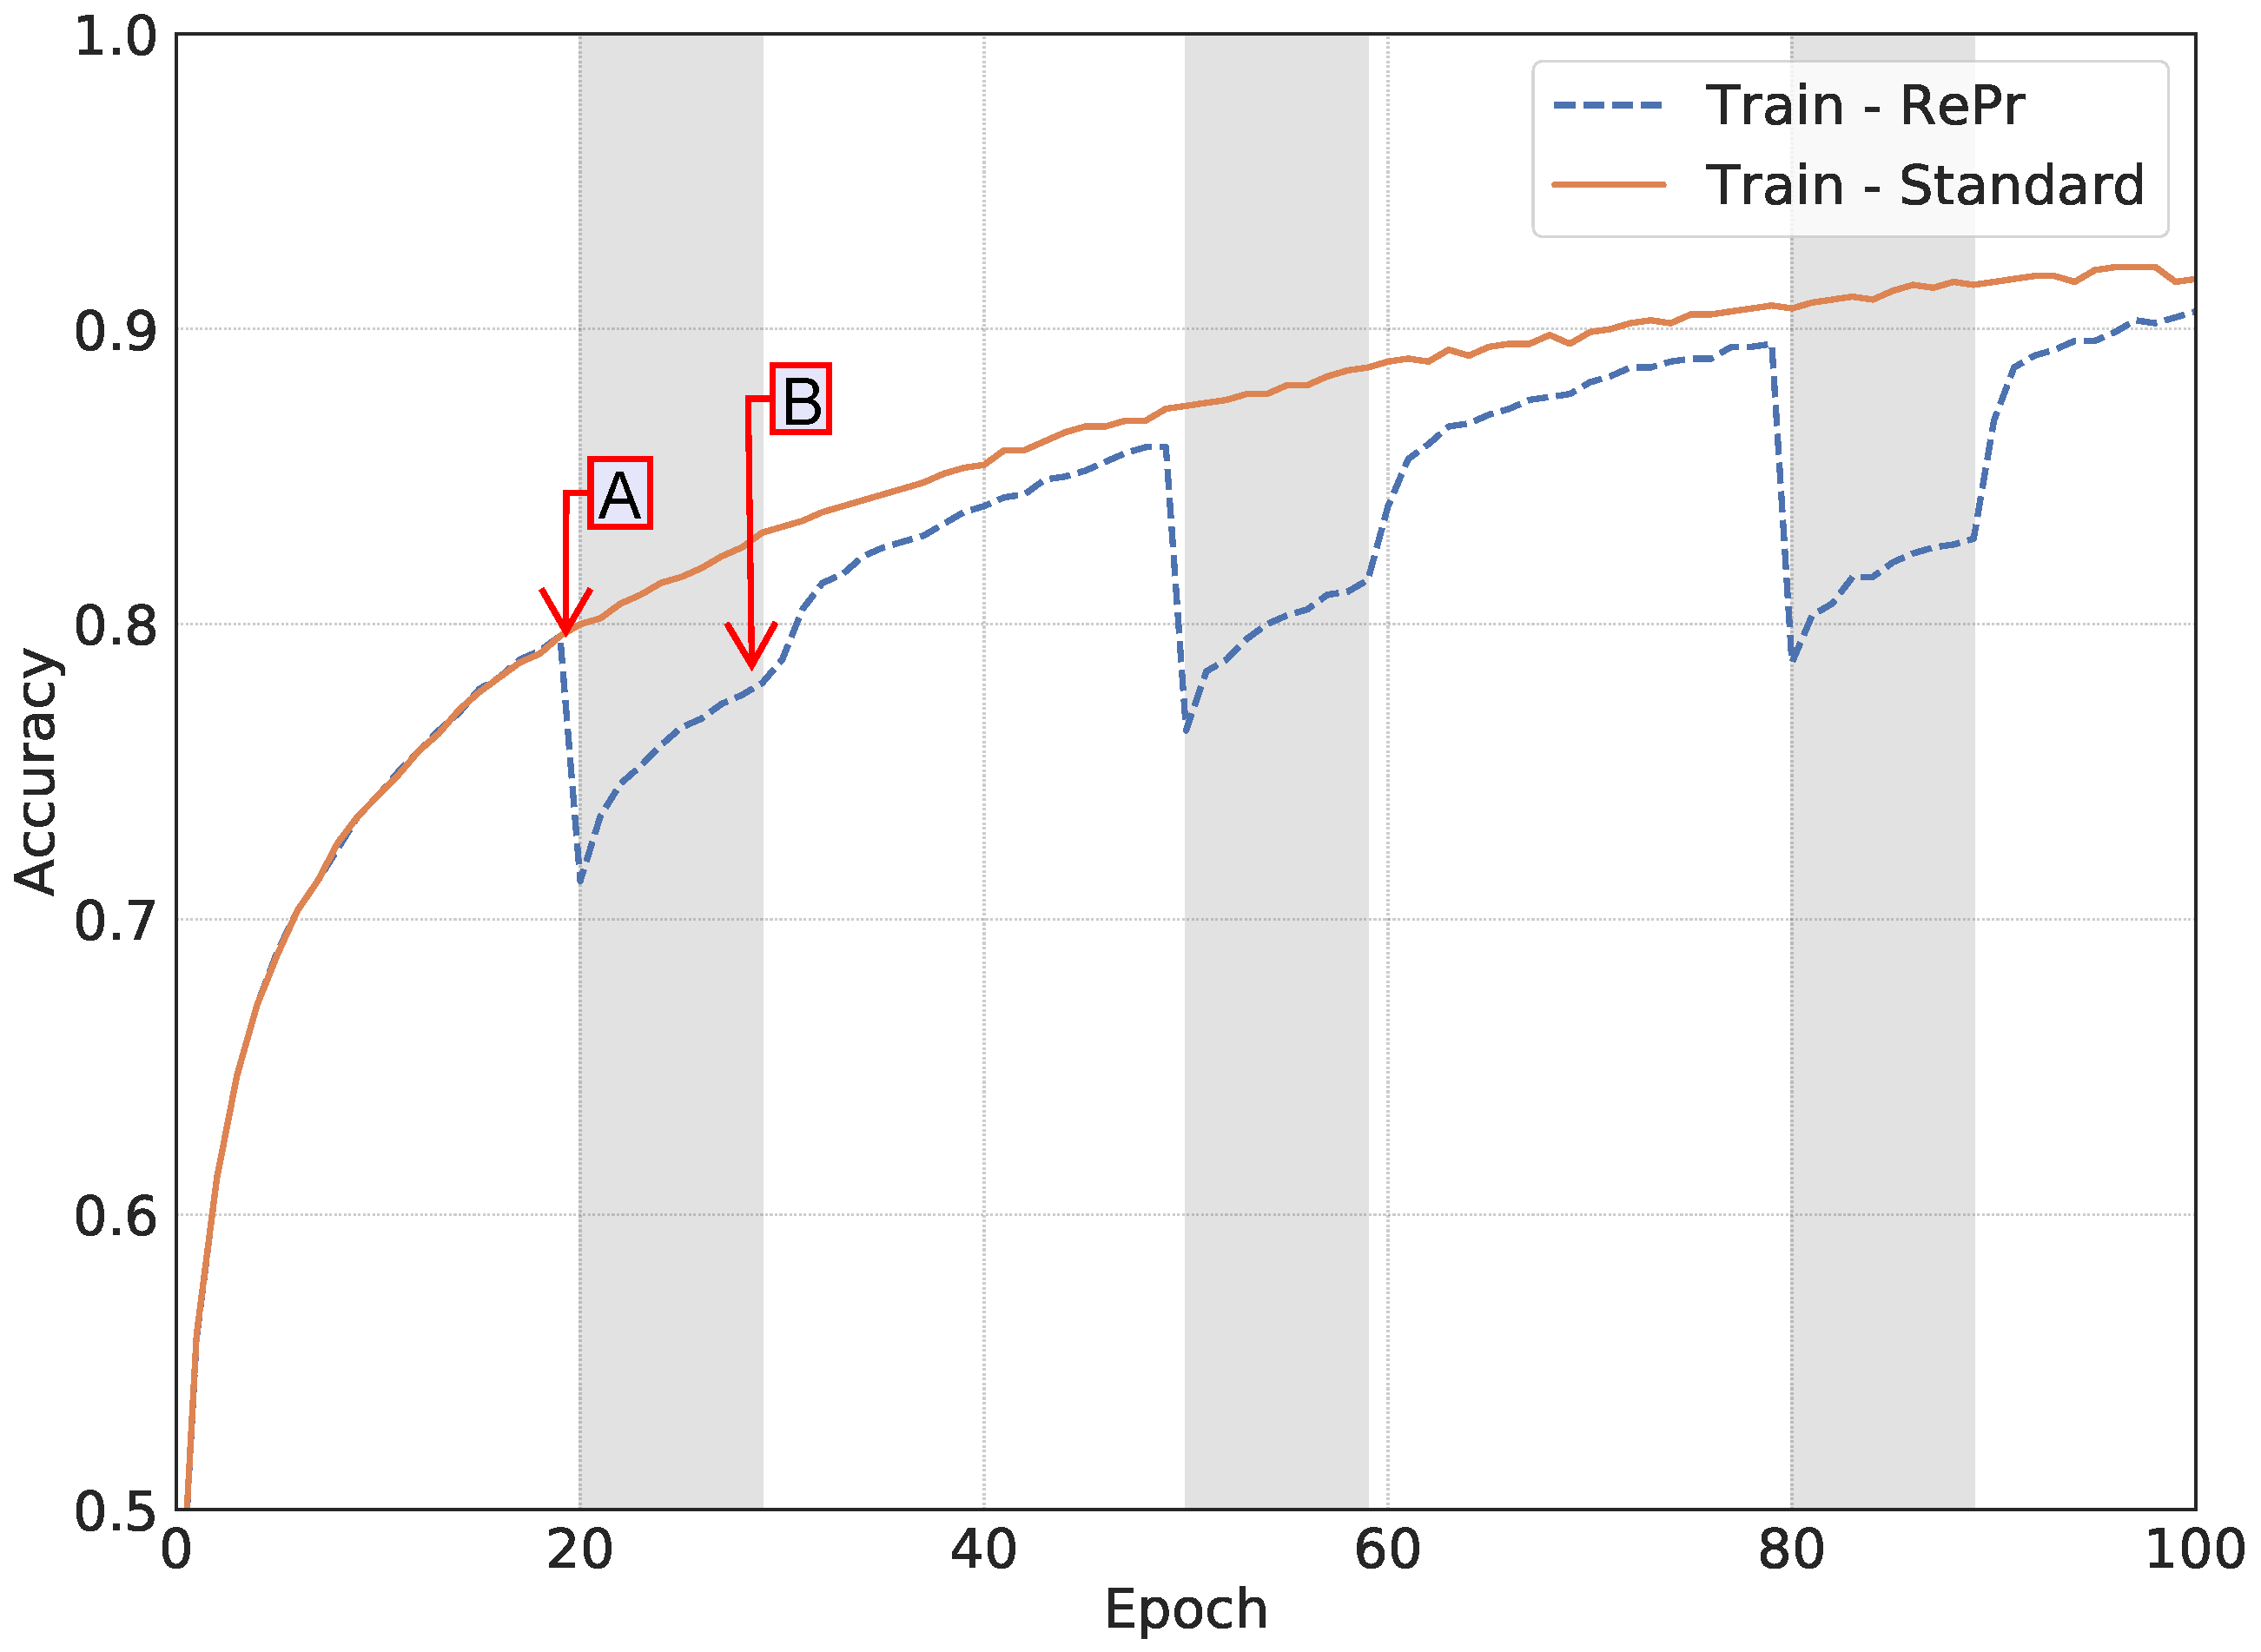
\includegraphics[width=0.47\linewidth]{figures/repr/RePr_Train.pdf}
   %\hspace{-3.0mm}
   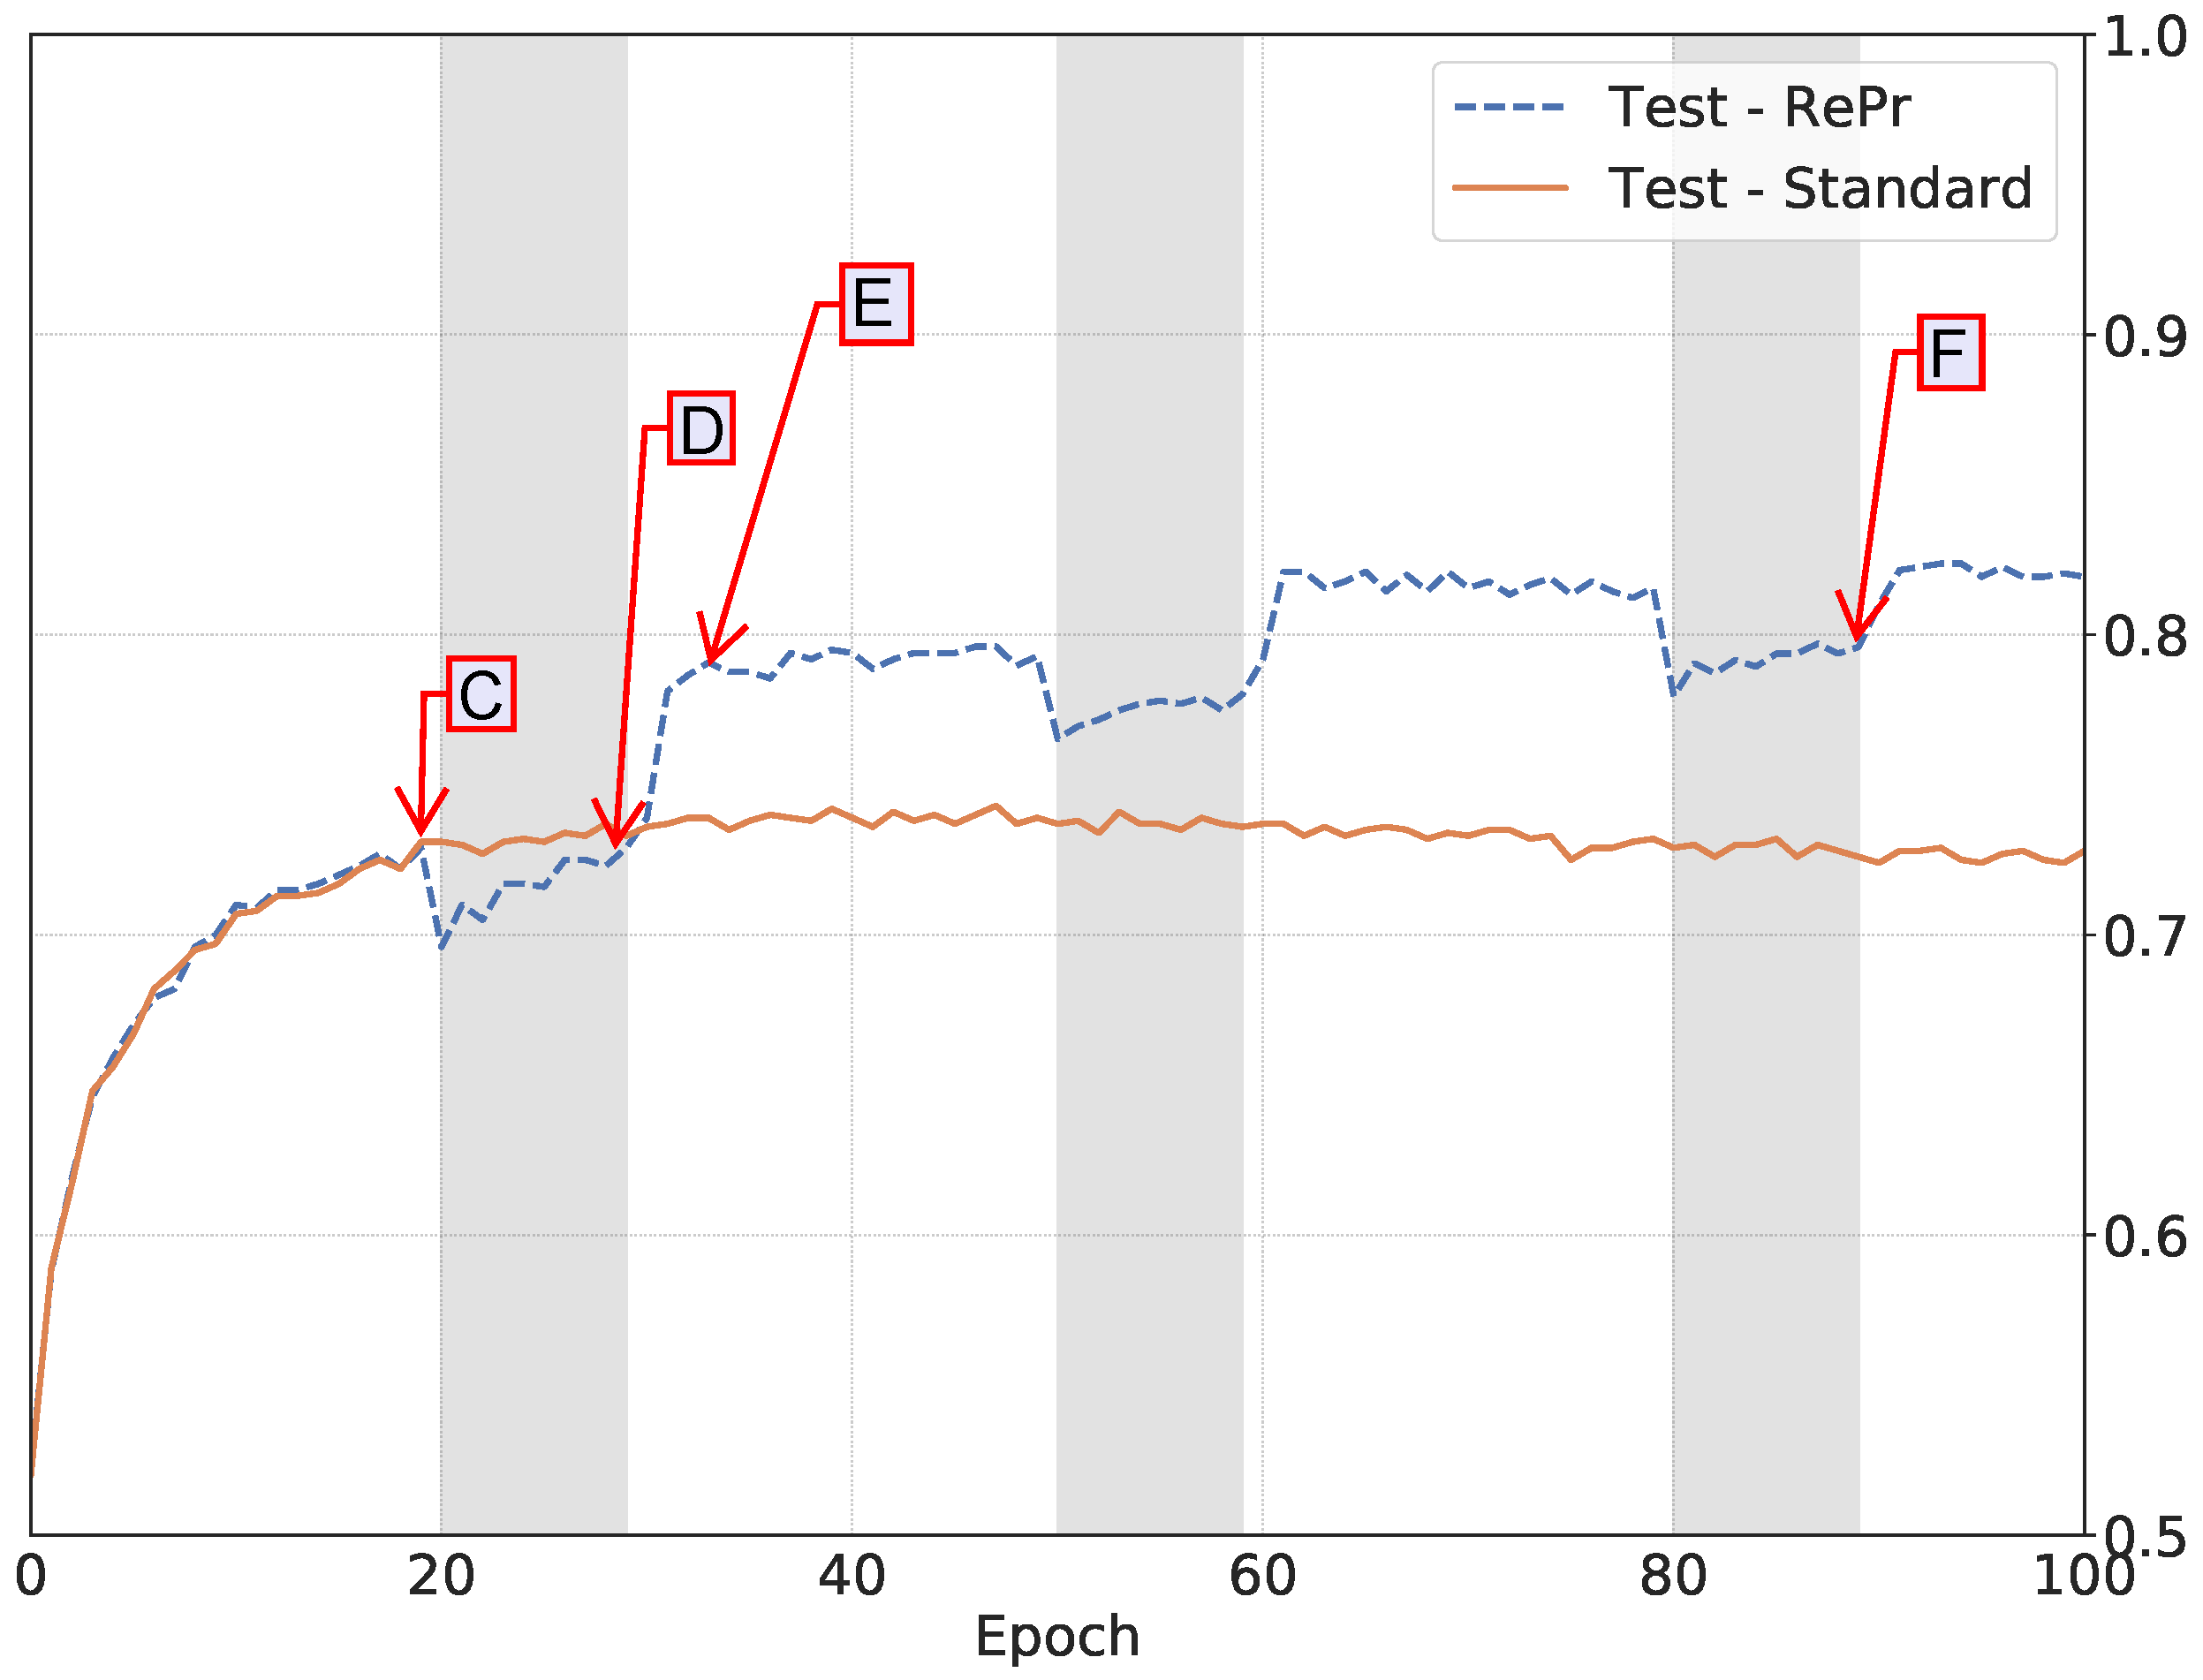
\includegraphics[width=0.45\linewidth]{figures/repr/RePr_Test.pdf}
   %\hspace{-8.0mm}
   %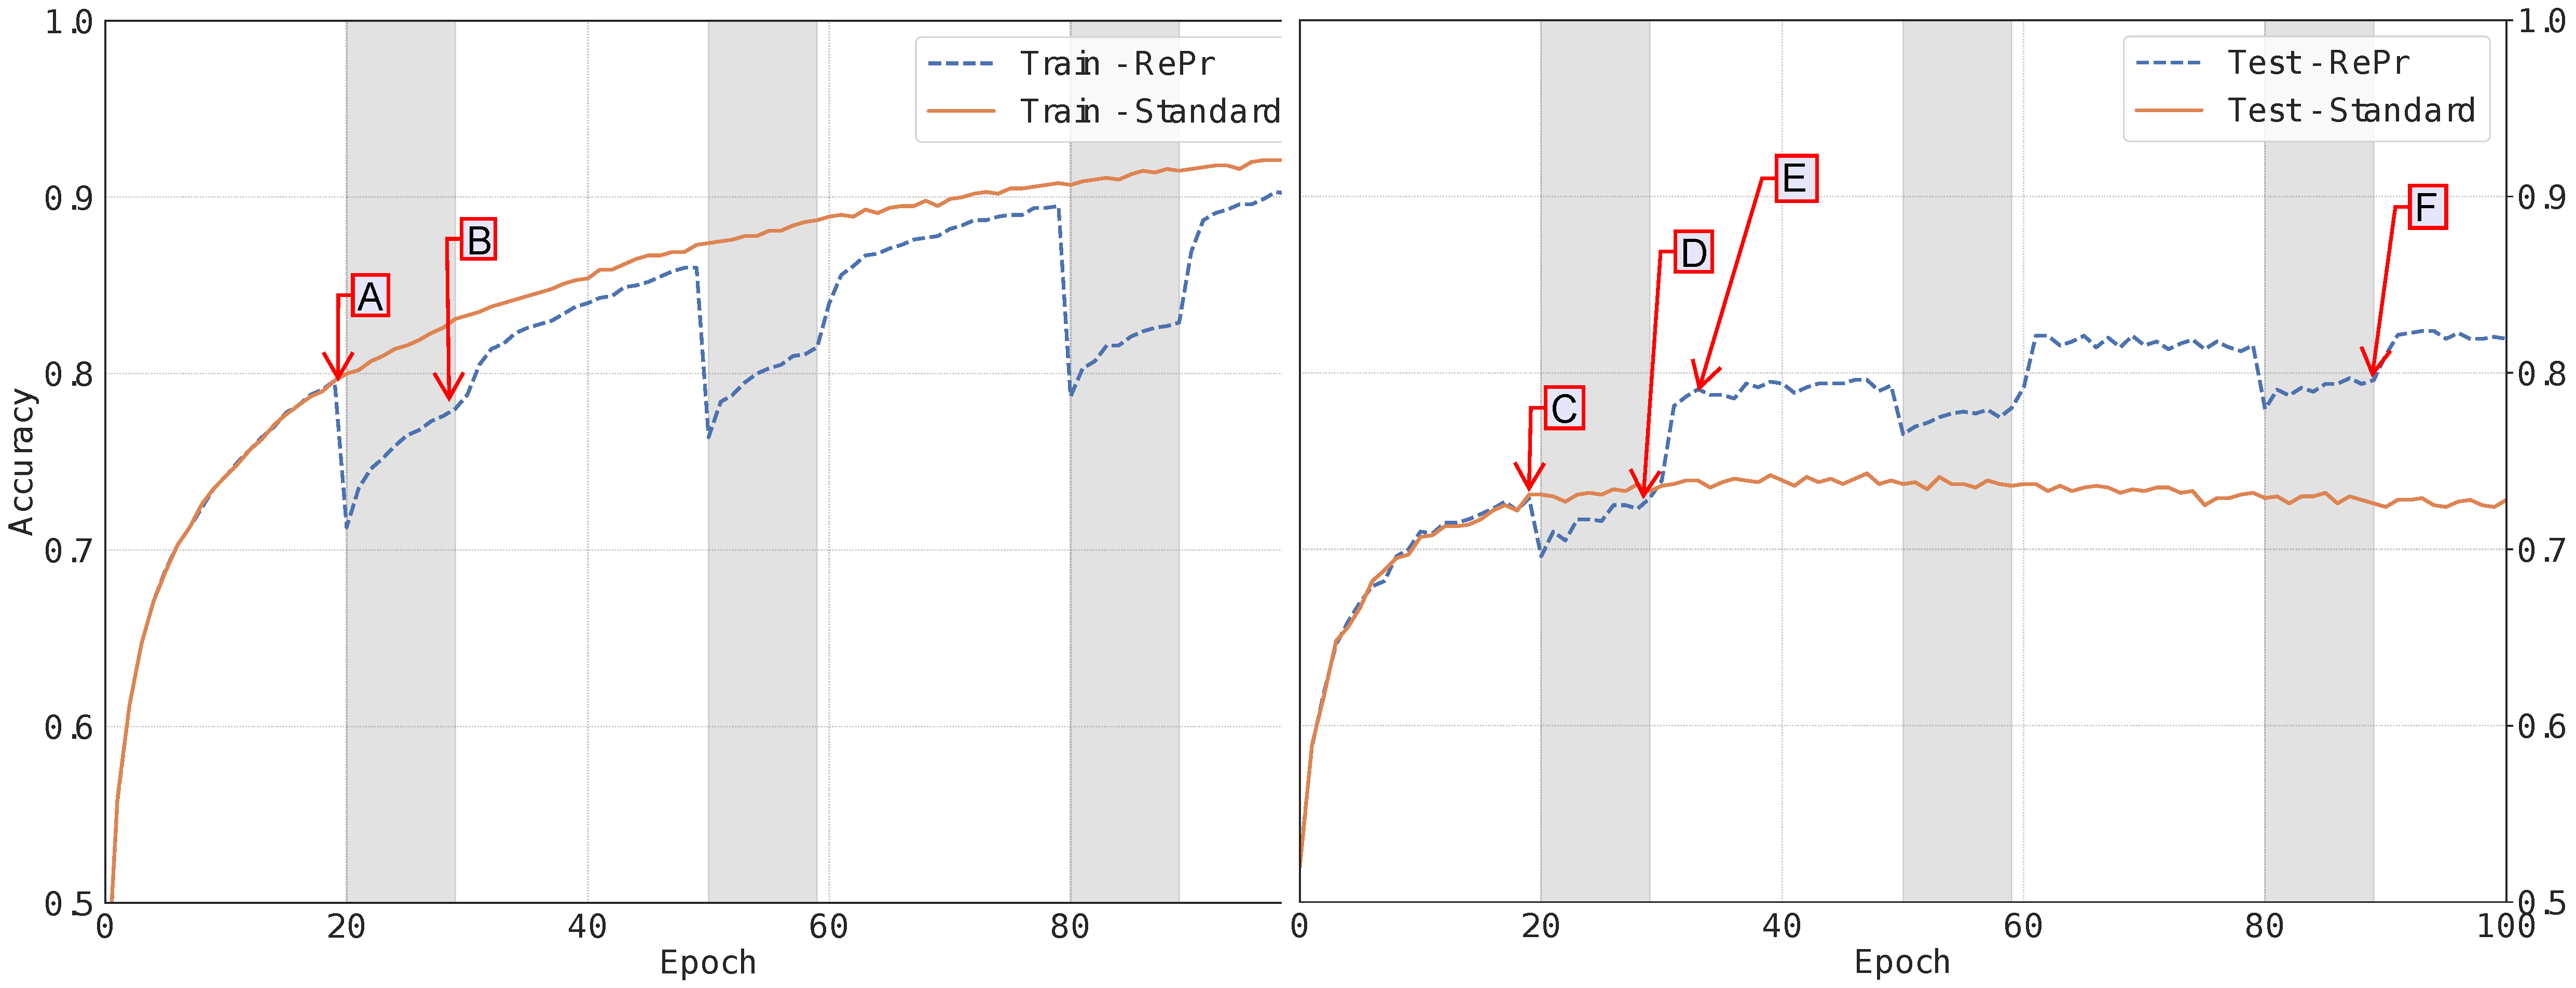
\includegraphics[width=1.05\linewidth]{figures/repr/combine_repr.pdf}
   %\vspace{-3mm}
   \caption[Performance Standard vs RePr]{Performance of a three layer ConvNet with 32 filters each over $100$ epochs using \textcolor{orange}{standard scheme} and \textcolor{blue}{our method - RePr} on CIFAR-$10$. The shaded regions denote periods when only part of the network is trained. 
   Left: Training Accuracy, Right: Test Accuracy. Annotations [A-F] are discussed in Section~\ref{sec:training}.}
   \label{fig:REPR}
   %%\vspace{1mm}
\end{figure}

%To that aim, we suggest a training scheme whereby after certain iterations of standard training, we mark some percentage of filters based on pre-determined criteria and continue training the rest of the network temporarily without the marked filters. 
To this end, we propose a training scheme in which, after some number of iterations of standard training, we select a subset of the model's filters to be temporarily dropped.
%After few epochs of training the reduced network, we reintroduce the dropped filters with new starting weights. 
After additional training of the reduced network, we reintroduce the previously dropped filters, initialized with new weights, and continue standard training.
%On every the reintroduction of the dropped filters the model's performance jumps higher than the value before the drop. 
We observe that following the reintroduction of the dropped filters, the model is able to achieve higher performance than was obtained before the drop. 
Repeated application of this process obtains models which outperform those obtained by standard training as seen in Figure ~\ref{fig:REPR} and discussed in Section~\ref{sec:training}.
%Repeating this process a couple of times with diminishing returns yields a model that has improved performance compared to standard training alone. 
We observe this improvement across various tasks and over various types of convolutional networks.
%This training technique, regardless of the filter dropping criteria, in itself leads to improved performance.
This training procedure is able to produce improved performance across a range of possible criteria for choosing which filters to drop, and further gains can be achieved by careful selection of the ranking criterion.
According to a recent hypothesis~\cite{Frankle2018TheLT}, the relative success of over-parameterized networks may largely be due to an abundance of initial sub-networks.
%Our technique allows shallow models to seek larger space of sub-networks by repeated re-initialization.
Our method aims to preserve successful sub-networks while allowing the re-initialization of less useful filters.


%Both of these techniques benefit from giving parameters a second chance at initialization.
%Recently, this has been hypothesized to be a reason for the success of large networks over small ones~\cite{Frankle2018TheLT}.
%In addition to the training scheme a major contribution of our work is in exploring an efficient metric for temporary filter dropping that will lead to a model that significantly outperforms the standard training. 
In addition to our novel training strategy, the second major contribution of our work is an exploration of metrics to guide filter dropping.
%We show that ranking criteria used for filter pruning (permanent) is not the right choice, and does not malleable to our training scheme.
Our experiments demonstrate that standard techniques for permanent filter pruning are suboptimal in our setting, and we present an alternative metric which can be efficiently computed, and which gives a significant improvement in performance.
%We propose a metric based on the \textit{inter-}filter orthogonality of convolutional layers as the most effective ranking measure for this alternative training scheme. 
We propose a metric based on the \textit{inter-}filter orthogonality within convolutional layers and show that this metric outperforms state-of-the-art filter importance ranking methods used for network pruning in the context of our training strategy.
%We explore most of the widely known and state-of-the-art filter importance ranking criteria used for pruning networks and show that our metric out-performs all of them while keeping the computation cost on the lower side.
%Several researchers have observed that ConvNets learn over-lapping representations and have redundant filters~\cite{Cogswell2015ReducingOI, Li2016PruningFF}.
We observe that even small, under-parameterized networks tend to learn redundant filters, which suggests that filter redundancy is not solely a result of over-parameterization, but is also due to ineffective training.
%We observed that this is also true for shallow networks and not just deep networks.
%Thus the redundancy is not necessarily due to over-parameterization but also to some extent due to ineffective training.
Our goal is to reduce the redundancy of the filters and increase the expressive capacity of ConvNets and we achieve this by changing the training scheme rather than the model architecture.



\section{Related Work}

%We have divided the discussion of related works into categories that broadly cover our area of research.
\subsection{Training Scheme } 
Many changes to the training paradigm have been proposed to reduce over-fitting and improve generalization.
Dropout~\cite{Wu2015TowardsDT} is widely used in training deep nets. 
By stochastically dropping the neurons it prevents co-adaption of feature detectors.
A similar effect can be achieved by dropping a subset of activations ~\cite{Wan2013RegularizationON}.
Wu \etal~\cite{Wu2015TowardsDT} extend the idea of stochastic dropping to convolutional neural networks by probabilistic pooling of convolution activations.
Yet another form of stochastic training recommends randomly dropping entire layers~\cite{Huang2016DeepNW}, forcing the model to learn similar features across various layers which prevent extreme overfitting.
In contrast, our technique encourages the model to use a linear combination of features instead of duplicating the same feature.
Han \etal~\cite{Han2016DSDDT} propose Dense-Sparse-Dense (DSD), a similar training scheme, in which they apply weight regularization mid-training to encourage the development of sparse weights, and subsequently remove the regularization to restore dense weights.
They recommend adding weight regularization to make sparse weights and removing the regularization subsequently to achieve dense network again.
DSD works on individual parameters and uses weight norm to drop the weights. 
We designed our training scheme for specially convolutional filters and we show that it is important to allow each of the model (with reduced filters) to converge before switching over. 
While DSD works at the level of individual parameters, our method is specifically designed to apply to convolutional filters.
We achieve this by allowing the sub-network to relearn any missing feature representations with existing filters.
In a limited model capacity, doing so encourages more expressivity~\cite{Raghu2017OnTE} and as our results show it leads to efficient model.



\subsection{Model Compression } 
Knowledge Distillation (KD)~\cite{Hinton2015DistillingTK} is a training scheme which uses soft logits from a larger trained model (teacher) to train a smaller model (student).
Soft logits capture hierarchical information about the object and provide a smoother loss function for optimization. This leads to easier training and better convergence for small models.
Stronger forms of KD where a model matches intermediate activations have also been proposed~\cite{Romero2014FitNetsHF}. 
By forcing the student model to match the output statistics from the teacher, it provides the directions for weight updates which are not found in the gradients.
In a surprising result, Born-Again-Network~\cite{Furlanello2018BornAN} shows that if the student model is of the same capacity as the teacher it can outperform the teacher.
A few other variants of KD have been proposed~\cite{Romero2014FitNetsHF} and all of them require training several models.
Our training scheme does not depend on an external teacher and requires less training than KD. %More importantly, our scheme is complementary to KD. 
More importantly, when combined with KD, our method gives better performance than can be achieved by either technique independently (discussed in Section~\ref{lbl:distillation}).


\subsection{Neuron ranking }
Interest in finding the least salient neurons/weights has a long history. 
LeCun~\cite{LeCun1989OptimalBD} and Hassibi\etal~\cite{Hassibi1992SecondOD} show that using the Hessian, which contains second-order derivative, identifies the weak neurons and performs better than using the magnitude of the weights.
Computing the Hessian is expensive and thus is not widely used.
Han \etal~\cite{Han2015DeepCC} show that the norm of weights is still effective ranking criteria and yields sparse models.
The sparse models do not translate to faster inference, but as a neuron ranking criterion, they are effective.
Computing the norm of the weights is easy and data-free, thus lends itself to pruning for transfer learning.
Hu \etal~\cite{Hu2016NetworkTA} explore Average Percentage of Zeros (APoZ) in the activations and use a data-driven threshold to determine the cut-off. 
It is a useful comparison metric and works well when the training data is available.
ThinNet~\cite{Luo2017ThiNetAF} explores reconstruction error between the layers, this does not lead to a generalized filter ranking criteria.
Molchanov \etal~\cite{Molchanov2016PruningCN} recommend the second term from the Taylor expansion of the loss function.%, which is a product of activation and the gradient.
Currently, it is the state-of-the-art in filter pruning and works well for transfer pruning.
Our filter ranking criteria, \textit{inter}-filter orthogonality, is yet another approach and is designed especially for the purposes of temporary pruning. 
We provide detail comparison and show results on using these metrics with our training scheme in Section~\ref{sec:metric}.

Chen \etal ~\cite{Chen2017TrainingGO} used privileged information, like segmentation maps, to encourage diversity in feature maps, and approximate group orthogonal filters.
Unfortunately, such techniques restrict themselves to domains where segmentation maps are available for the task of image classification. 
Our method does not rely on any external information or a pretrained model.

\subsection{Architecture Search } 

Neural architecture search ~\cite{Liu2017ProgressiveNA, Real2018RegularizedEF, Zoph2016NeuralAS} is where the architecture is modified during training, and multiple neural network structures are explored in search of the best architecture for a given dataset. 
Such methods do not have any benefits if the architecture is fixed ahead of time. Our scheme improves training for a given architecture by making better use of the available parameters. 
This could be used in conjunction with architecture search if there is flexibility around the final architecture or used on its own when the architecture is fixed due to certified model deployment, memory requirements, or other considerations.
Our scheme is finds better weights given a fixed architecture and thus have a lower potential than the NAS models.
Potential for finding a better generalizing architecture diminishes by restricting to a fixed final architecture but asserts itself to several applications where predetermined architecture is warranted.
This could be due to certified model deployment, memory requirements or better interpretability of simpler ConvNets.

\subsection{Feature correlation } 
A well-known shortcoming of vanilla convolutional networks is their correlated feature maps~\cite{Cogswell2015ReducingOI, Glorot2010UnderstandingTD}.
Architectures like Inception-Net~\cite{Szegedy2015GoingDW} are motivated by analyzing the correlation statistics of features across layers.
They aim to reduce the correlation between the layers by using concatenated features from various sized filters, subsequent research shows otherwise~\cite{Raghu2017SVCCASV}.
%However, correlation of singular values across inception layers show that there is a significant overlap of activations. 
More recent architectures like ResNet~\cite{he2015deep} and DenseNet ~\cite{Huang2017DenselyCC} aim to implicitly reduce feature correlations by summing or concatenating activations from previous layers.
That said, these models are computationally expensive and require large memory to store previous activations.
Our aim is to induce decorrelated features without changing the architecture of the convolutional network.
This benefits all the existing implementations of ConvNet without having to change the infrastructure.
While our technique performs best with vanilla ConvNet architectures it still marginally improves the performance of modern architectures.

\section{Motivation for Orthogonal Features}
A feature for a convolutional filter is defined as the point-wise sum of the activations from individual kernels of the filter.
A feature is considered useful if it helps to improve the generalization of the model.
A model that has poor generalization usually has features that, in aggregate, capture limited directions in activation space~\cite{Morcos2017OnTI}.
%If the features are orthogonal they will be less correlated and capture more of the directions.
On the other hand, if a model's features are orthogonal to one another, they will each capture distinct directions in activation space, leading to improved generalization.
%For a trivial sized ConvNet, maximally expressive weights is computed by analyzing the correlation of features across layers and clustering them to common groups~\cite{Arora2014ProvableBF}. 
For a trivially-sized ConvNet, we can compute the maximally expressive filters by analyzing the correlation of features across layers and clustering them into groups~\cite{Arora2014ProvableBF}.
%However, this scheme for finding weights is impractical for a typical sized deep ConvNet. 
However, this scheme is computationally impractical for the deep ConvNets used in real-world applications.
%Instead of adding a regularization during standard SGD training minimizes the covariance of activations leads to slightly better models~\cite{Rodrguez2016RegularizingCW, Cogswell2015ReducingOI}.
Alternatively, a computationally feasible option is the addition of a regularization term to the loss function used in standard SGD training which encourages the minimization of the covariance of the activations, but this produces only limited improvement in model performance~\cite{Rodrguez2016RegularizingCW, Cogswell2015ReducingOI}.
%Similarly, marginal improvements have been observed by regularizing the orthogonality of weights during training~\cite{Brock2016NeuralPE, Poole2014AnalyzingNI, Xie2017NearOrthogonalityRI}.
A similar method, in which the regularization term instead encourages the orthogonality of filter weights, has also produced marginal improvements~\cite{Brock2016NeuralPE, Poole2014AnalyzingNI, Xie2017NearOrthogonalityRI, Xie2017AllYN}.
Shang \etal~\cite{Shang2016UnderstandingAI} discovered the low-level filters are duplicated with opposite phase. 
%This can be prevented by using CReLU in place of ReLU, but the later still remains the most common choice for the activation function.
Forcing filters to be orthogonal will minimize this duplication without changing the activation function.
%These techniques fall short of finding the filters that are perfectly decorrelated but are practical for everyday use.
%An another advantage of weights being orthogonal are that they lead to stable convergence of deep networks~\cite{Saxe2013ExactST}.
In addition to improvements in performance and generalization, Saxe \etal ~\cite{Saxe2013ExactST} show that the orthogonality of weights also improves the stability of network convergence during training.
The authors of ~\cite{Xie2017AllYN, Xiao2018DynamicalIA} further demonstrate the value of orthogonal weights to the efficient training of networks.
%This is also why Recurrent Neural Networks are often initialized with orthogonal weights due to their sensitivity of initial point~\cite{Vorontsov2017OnOA} even if this is no longer popular for ConvNets.
Orthogonal initialization is common practice for Recurrent Neural Networks due to their increased sensitivity to initial conditions~\cite{Vorontsov2017OnOA}, but it has somewhat fallen out of favor for ConvNets.
%Yet another advantage of orthogonal weights is that they lead to the efficient training of very deep networks~\cite{Xie2017AllYN, Xiao2018DynamicalIA}.
These factors shape our motivation for encouraging orthogonality of features in the ConvNet and form the basis of our ranking criteria.

Collecting activations over a dataset in order to compute orthogonal features is slow and inefficient. Instead, we use orthogonality of weights, to represent feature overlap.
Because features are dependent on the input data, determining their orthogonality requires computing statistics across the entire training set, and is therefore prohibitive.  
We instead compute the orthogonality of filter weights as a surrogate.
Our experiments show that encouraging weight orthogonality through a regularization term is insufficient to promote the development of features which capture the full space of the input data manifold.
Our method of dropping overlapping filters acts as an implicit regularization and leads to the better orthogonality of filters without hampering model convergence.


We use Canonical Correlation Analysis~\cite{hotelling1936relations} (CCA) to study the overlap of features in a single layer.
CCA finds the linear combinations of random variables that show maximum correlation with each other.
It is a useful tool to determine if the learned features are overlapping in their representational capacity. 
Li \etal ~\cite{Li2015ConvergentLD} apply correlation analysis to filter activations to show that most of the well-known ConvNet architectures learn similar representations.
Raghu \etal ~\cite{Raghu2017SVCCASV} combine CCA with SVD to perform a correlation analysis of the singular values of activations from various layers.
They show that increasing the depth of a model does not always lead to a corresponding increase of the model's dimensionality, due to several layers learning representations in correlated directions.
We ask an even more elementary question - how correlated are the activations from various filters within a single layer?
In an over-parameterized network like VGG-$16$, which has several convolutional layers with $512$ filters each, it is no surprise that most of the filter activations are highly correlated.
%Thus, it is one of the easily pruned networks with models achieving same performance after dropping over $50$\% of the filters~\cite{Molchanov2016PruningCN, Li2015ConvergentLD}.
As a result, VGG-$16$ has been shown to be easily pruned - more than $50$\% of the filters can be dropped while maintaining the performance of the full network~\cite{Molchanov2016PruningCN, Li2015ConvergentLD}.
Is this also true for significantly smaller convolutional networks, which under-fit the dataset?


\begin{figure}[H]
   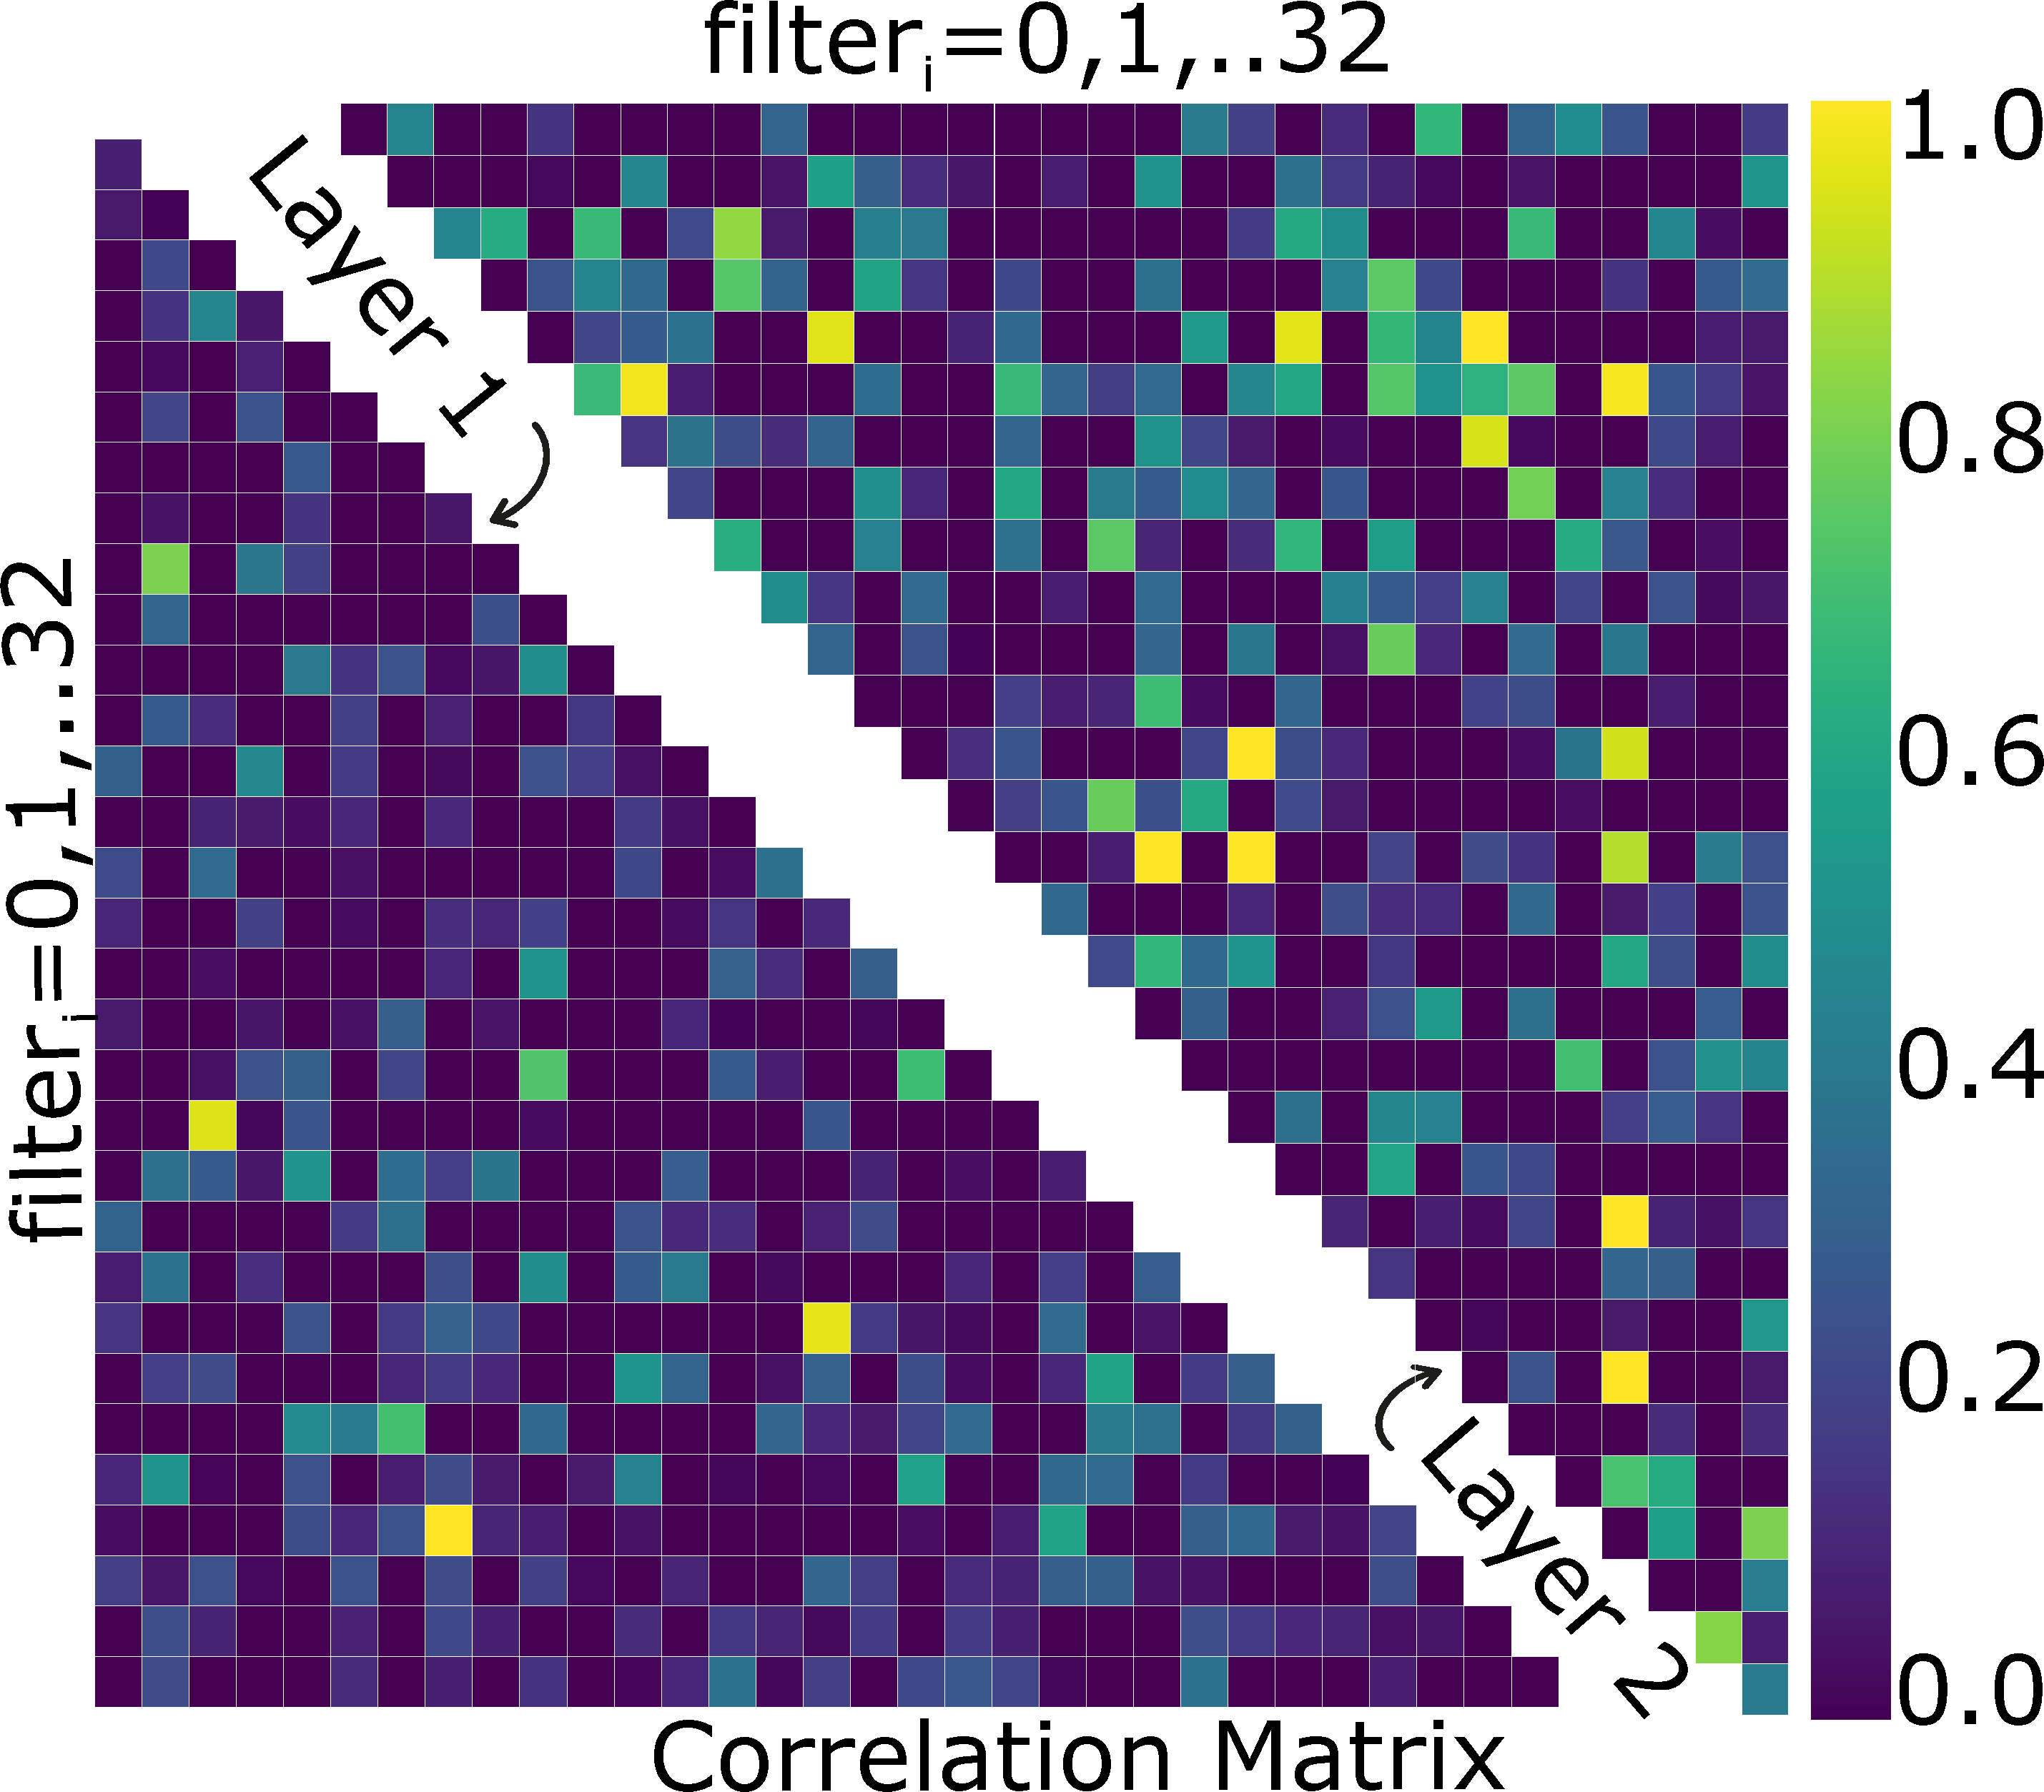
\includegraphics[width=0.49\linewidth]{figures/repr/Filter_CCA.pdf}
   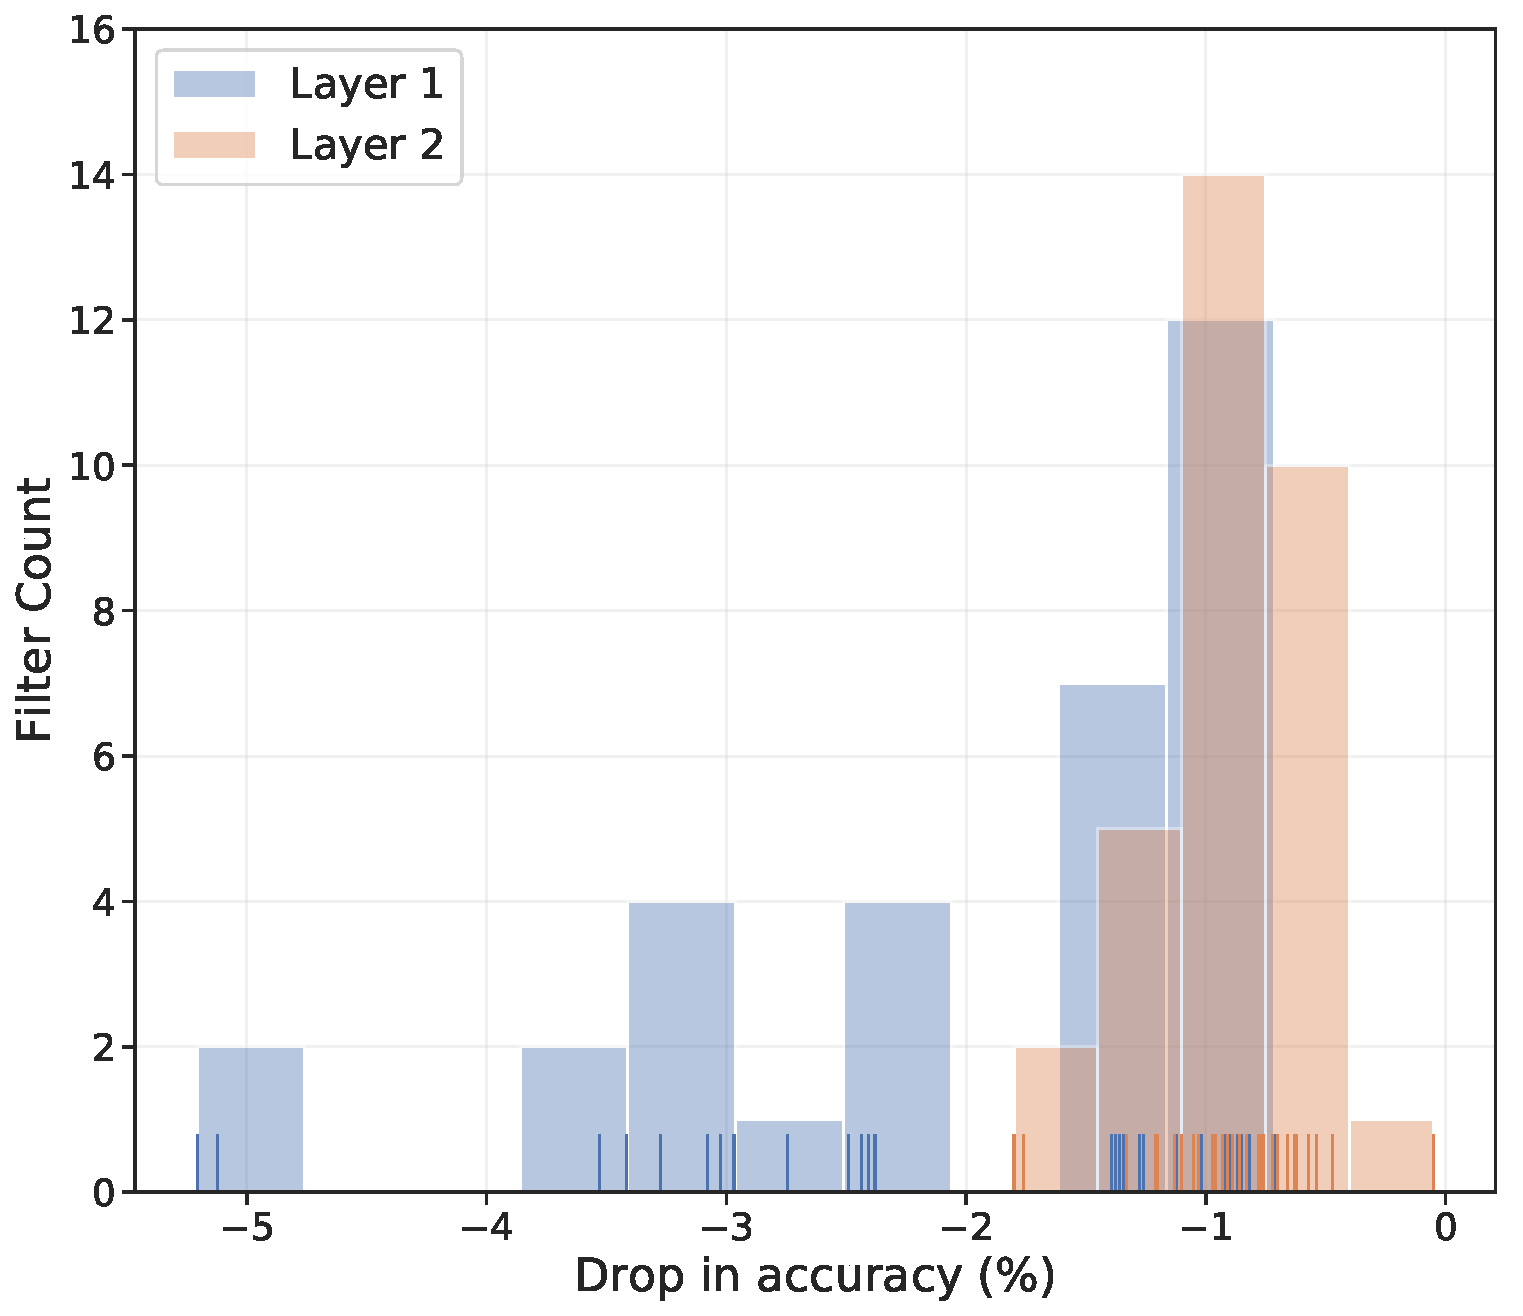
\includegraphics[width=0.49\linewidth]{figures/repr/Error_Distribution.pdf}
   %%\vspace{-2mm}
   \caption[Correlation Analysis of filters]{Left: Canonical Correlation Analysis of activations from two layers of a ConvNet trained on CIFAR-10. Right: Distribution of change in accuracy when the model is evaluated by dropping one filter at a time.}
   \label{fig:CCA}
   %\vspace{-2mm}
\end{figure}

We will consider a simple network with two convolutional layers of $32$ filters each, and a softmax layer at the end.
Training this model on CIFAR-$10$ for $100$ epochs with an annealed learning rate results in test set accuracy of $58.2$\%, far below the $93.5$\% achieved by VGG-$16$.
%Given the limited capacity of this model every filter is critical to its performance and any correlation in activation would mean limited expressivity of the features and therefore inefficiency in the training.
In the case of VGG-$16$, we might expect that correlation between filters is merely an artifact of the over-parameterization of the model - the dataset simply does not have a dimensionality high enough to require every feature to be orthogonal to every other.
On the other hand, our small network has clearly failed to capture the full feature space of the training data, and thus any correlation between its filters is due to inefficiencies in training, rather than over-parameterization.

%, In order to measure the impact of each filter on the current performance we remove \textit{(zero out),} that filter and run the inference on the test set.
Given a trained model, we can evaluate the contribution of each filter to the model's performance by removing \textit{(zeroing out)} that filter and measuring the drop in accuracy on the test set.
We will call this metric of filter importance the \emph{"greedy Oracle"}.
We perform this evaluation independently for every filter in the model, and plot the distribution of the resulting drops in accuracy in Figure~\ref{fig:CCA} (right).
%We run this independently for all the filters and show the distribution of drop in accuracy due to removing each of the filters in figure~\ref{fig:CCA} (right). This kind of filter importance ranking is known as greedy Oracle.
Most of the second layer filters contribute less than $1\%$ in accuracy and with first layer filters, there is a long tail. 
Some filters are important and contribute over $4\%$ of accuracy but most filters are around $1\%$. 
This implies that even a tiny and under-performing network could be filter pruned without significant performance loss.
The model has not efficiently allocated filters to capture wider representations of necessary features. 
Figure ~\ref{fig:CCA} (left) shows the correlations from linear combinations of the filter activations (CCA) at both the layers.
It is evident that in both the layers there is a significant correlation among filter activations with several of them close to a near perfect correlation of $1$ (\textit{bright yellow spots} $\color{Yellow} \blacksquare$).  The second layer (upper right diagonal) has lot more overlap of features the first layer (lower right).
For a random orthogonal matrix any value above $0.3$ (\textit{lighter than dark blue} $\color{blue} \blacksquare$) is an anomaly.
The activations are even more correlated if the linear combinations are extended to kernel functions~\cite{Hardoon2004CanonicalCA} or singular values~\cite{Raghu2017SVCCASV}.
Regardless, it suffices to say that standard training for convolutional filters does not maximize the representational potential of the network.



 


\section{Our Training Scheme : RePr} \label{sec:training}

We modify the training process by cyclically removing redundant filters, retraining the network, re-initializing the removed filters, and repeating. 
%In order to determine the redundancy of a filter within its layer, we first flatten the $3$D filters into $1$D vectors and correlate them against one another.
We consider each filter ($3$D\textit{ tensor}) as a single unit, and represent it as a long vector - ($f$).
Let $\mathbf{M}$ denote a model with $\mathcal{F}$ filters spread across $\mathbf{L}$ layers. 
Let $\mathcal{\widehat{F}}$ denote a subset of $\mathcal{F}$ filters, such that $\mathbf{M}_\mathcal{F}$ denotes a complete network whereas, $\mathbf{M}_\mathcal{F-\widehat{F}}$ denotes a sub-network without that $\mathcal{\widehat{F}}$ filters.
Our training scheme alternates between training the complete network ($\mathbf{M}_\mathcal{F}$) and the sub-network ($\mathbf{M}_\mathcal{F-\widehat{F}}$).
This introduces two hyper-parameters.
First is the number of iterations to train each of the networks before switching over; let this be $S_1$ for the full network and $S_2$ for the sub-network. 
%If $S_1$ and $S_2$ are equal to $1$, then this scheme becomes stochastic dropout of filters. 
These have to be non-trivial values so that each of the networks learns to improve upon the results of the previous network.
The second hyper-parameter is the total number of times to repeat this alternating scheme; let it be $N$. 
This value has minimal impact beyond certain range and does not require tuning.


The most important part of our algorithm is the metric used to rank the filters. 
Let $\mathcal{R}$ be the metric which associates some numeric value to a filter. 
This could be a norm of the weights or its gradients or our metric - \textit{inter-}filter orthogonality in a layer.
Here we present our algorithm agnostic to the choice of metric. Most sensible choices for filter importance results in an improvement over standard training when applied to our training scheme \textit{(see Ablation Study~\ref{sec:ablation})}.
%We provide a detailed description of our metric and its comparison in the sections below.


Our training scheme operates on a macro-level and is not a weight update rule.
Thus, is not a substitute for SGD or other adaptive methods like Adam~\cite{Kingma2014AdamAM} and RmsProp~\cite{Tieleman2012}. 
Our scheme works with any of the available optimizers and shows improvement across the board. %TODO table reference
However, if using an optimizer that has parameters specific learning rates \textit{(like Adam)}, it is important to re-initialize the learning rates corresponding to the weights
that are part of the pruned filters ($\mathcal{\widehat{F}}$).
Corresponding Batch Normalization~\cite{Ioffe2015BatchNA} parameters ($\gamma \& \beta$) must also be re-initialized.
For this reason, comparisons of our training scheme with standard training are done with a common optimizer.
%TODO add table for optimizer comparison

%We reinitialize the filters ($\mathcal{\widehat{F}}$) to be orthogonal to its value before being dropped and the current value of non-pruned filters ($\mathcal{F-\widehat{F}}$).

Our algorithm is training interposed with \textbf{Re}-initializing and \textbf{Pr}uning - \textbf{RePr} \textit{(pronounced: reaper)}.
We summarize our training scheme in Algorithm~\ref{alg:repr}.

\begin{algorithm}[H]
    \SetKwInOut{Input}{Input}
    \SetKwInOut{Output}{Output}
    %\For{$n\gets0$ \KwTo $N$}{
    \For{$N$ iterations}{
    
        \For{$S_1$ iterations}{
            Train the full network: $\mathbf{M}_\mathcal{F}$
        }
        
        Compute the metric : $\mathcal{R}(f) \  \forall f\in \mathcal{F}$
        
        Let $\mathcal{\widehat{F}}$ be bottom $p_\%$ of $\mathcal{F}$ using $\mathcal{R}(f)$
        
        \For{$S_2$ iterations}{
            Train the sub-network : $\mathbf{M}_\mathcal{F-\widehat{F}}$
        }
        
        Reinitialize the filters ($\mathcal{\widehat{F}}$) s.t. $\mathcal{\widehat{F}} \perp \mathcal{F}$
        
        {\textit{(and their training specific parameters \\ from BatchNorm and Adam, if applicable)}}
        
    }
    \caption[RePr Training Scheme]{RePr Training Scheme}
    \label{alg:repr}
\end{algorithm}

We use a shallow model to analyze the dynamics of our training scheme and its impact on the train/test accuracy. 
A shallow model will make it feasible to compute the greedy Oracle ranking for each of the filters.
This will allow us to understand the impact of training scheme alone without confounding the results due to the impact of ranking criteria.
We provide results on larger and deeper convolutional networks in Section Results~\ref{sec:results}.

%Consider a three layer vanilla ConvNet, without a skip or dense connections, as shown below.
Consider a $n$ layer vanilla ConvNet, without a skip or dense connections, with X filter each, as shown below:
\begin{equation*}  
    \text{Img} \longmapsto \bigg[ \text{CONV}(X) \rightarrow \text{RELU}  \bigg]^n \longmapsto \text{FC} \longmapsto \text{Softmax}
\end{equation*}

We will represent this architecture as $C^n(X)$. Thus, a $C^3(32)$ has $96$ filters, and when trained with SGD with a learning rate of $0.01$, achieves test accuracy of $73\%$.
Figure~\ref{fig:REPR} shows training plots for accuracy on the training set (left) and test set (right). 
In this example, we use a RePr training scheme with $S_1=20, S_2=10, N=3, p_\%=30$ and the ranking criteria $\mathcal{R}$ as a greedy Oracle.
We exclude a separate validation set of $5$K images from the training set to compute the Oracle ranking.
In the training plot, annotation [A] shows the point at which the filters are first pruned.
Annotation [C] marks the test accuracy of the model at this point. 
The drop in test accuracy at [C] is lower than that of training accuracy at [A], which is not a surprise as most models overfit the training set.
However, the test accuracy at [D] is the same as [C] but at this point, the model only has $70\%$ of the filters. 
This is not a surprising result, as research on filter pruning shows that at lower rates of pruning most if not all of the performance can be recovered~\cite{Molchanov2016PruningCN}.

What is surprising is that test accuracy at [E], which is only a couple of epochs after re-introducing the pruned filters, is significantly higher than point [C].
Both point [C] and point [E] are same capacity networks, and higher accuracy at [E] is not due to the model convergence. 
In the standard training (\textcolor{orange}{orange line}) the test accuracy does not change during this period.
Models that first grow the network and then prune~\cite{Dai2017NeSTAN, Han2015LearningBW}, unfortunately, stopped shy of another phase of growth, which yields improved performance. 
In their defense, this technique defeats the purpose of obtaining a smaller network by pruning. 
However, if we continue RePr training for another two iterations, we see that the point [F], which is still at $70\%$ of the original filters yields accuracy which is comparable
to the point [E] ($100\%$ of the model size.

Another observation we can make from the plots is that training accuracy of RePr model is lower, which signifies some form of regularization on the model. 
This is evident in the Figure~\ref{fig:ablation_percent} (Right), which shows RePr with a large number of iterations ($N=28$). 
While the marginal benefit of higher test accuracy diminishes quickly, the generalization gap between train and test accuracy is reduced significantly.


\section{Our Metric : \textit{inter}-filter orthogonality} \label{sec:metric}

The goals of searching for a metric to rank least important filters are twofold - (1) computing the greedy Oracle is not computationally feasible for large networks, and (2) the greedy Oracle may not be the best criteria. If a filter which captures a unique direction, thus not replaceable by a linear combination of other filters, has a lower contribution to accuracy, the Oracle will drop that filter. On a subsequent re-initialization and training, we may not get back the same set of directions.

The directions captured by the activation pattern expresses the capacity of a deep network~\cite{Raghu2017OnTE}. 
Making orthogonal features will maximize the directions captured and thus expressiveness of the network.
In a densely connected layer, orthogonal weights lead to orthogonal features, even in the presence of ReLU~\cite{Vorontsov2017OnOA}.
However, it is not clear how to compute the orthogonality of a convolutional layer. 

%A parameter of a Convolutional layer is a group of a single kernel, which is only sparsely connected to the previous layer.
A convolutional layer is composed of parameters grouped into spatial kernels and sparsely share the incoming activations.
Should all the parameters in a single convolutional layer be considered while accounting for orthogonality?
The theory that promotes initializing weights to be orthogonal is based on densely connected layers (FC-layers) and popular deep learning libraries follow this guide\footnote{tensorflow:ops/init\_ops.py\#L543 \& pytorch:nn/init.py\#L350} by considering convolutional layer as one giant vector disregarding the sparse connectivity.
A recent attempt to study orthogonality of convolutional filters is described in ~\cite{Xiao2018DynamicalIA} but their motivation is the convergence of very deep networks (10K layers) and not orthogonality of the features.
Our empirical study suggests a strong preference for requiring orthogonality of individual filters in a layer (inter-filter \& intra-layer) rather than individual kernels.


A filter of kernel size $k\times k$ is commonly a $3$D tensor of shape $k \times k \times c$, where $c$ is the number of channels in the incoming activations.
Flatten this tensor to a $1$D vector of size $k*k*c$, and denote it by $f$.
%A convolutional layer usually has more than one filter per layer. 
Let $J_\ell$ denote the number of filters in the layer $\ell$, where $\ell \in \mathbf{L}$, and $\mathbf{L}$ is the number of layers in the ConvNet.
Let $\boldsymbol{W}_\ell$ be a matrix, such that the individual rows are the flattened filters ($f$) of the layer $\ell$.

Let $\boldsymbol{\hat{W}_\ell} = \boldsymbol{W_\ell}/||\boldsymbol{W_\ell}||$ denote the normalized weights.
Then, the measure of Orthogonality for filter $f$ in a layer $\ell$ (denoted by $O_\ell^f$) is computed as shown in the equations below.

% \begin{equation}
%     \boldsymbol{\hat{W}_\ell} = \frac{\boldsymbol{W_\ell}}{||\boldsymbol{W_\ell}||}
% \end{equation}

% \noindent\begin{minipage}{.5\linewidth}
% %\vspace{-1mm}
% \begin{equation}
% %\vspace{-1mm}
%   \boldsymbol{P}_\ell = |\boldsymbol{\hat{W}_\ell} \times \boldsymbol{\hat{W}_\ell}^T - I | 
% \end{equation}
% %\vspace{-0.2mm}
% \end{minipage}%
% \begin{minipage}{.5\linewidth}
% %\vspace{-1mm}
% \begin{equation}
% \label{eqn:ortho}
% %\vspace{-1mm}
%   O^f_\ell = \sum \boldsymbol{P_\ell}[f] / J_\ell
% \end{equation}
% %\vspace{-0.2mm}
% \end{minipage}

%\vspace{-3mm}
\begin{equation}
\boldsymbol{P}_\ell = |\boldsymbol{\hat{W}_\ell} \times \boldsymbol{\hat{W}_\ell}^T - I |
%\vspace{-3mm}
\end{equation}

\begin{equation}
\label{eqn:ortho}
O^f_\ell = \frac{\sum \boldsymbol{P_\ell}[f]}{J_\ell}
%\vspace{-3mm}
\end{equation}

$\boldsymbol{P}_\ell$ is a matrix of size $J_\ell \times J_\ell$ and $\boldsymbol{P}[i]$ denotes $i^{\textit{th}}$ row of $\boldsymbol{P}$.
Off-diagonal elements of a row of $\boldsymbol{P}$ for a filter $f$ denote projection of all the other filters in the same layer with $f$.
The sum of a row is minimum when other filters are orthogonal to this given filter.
We rank the filters least important (thus subject to pruning) if this value is largest among all the filters in the network.
While we compute the metric for a filter over a single layer, the ranking is computed over all the filters in the network.
We do not enforce per layer rank because that would require learning a hyper-parameter $p_\%$ for every layer and some layers are more sensitive than others.
Our method prunes more filters from deeper layers compared to the earlier layers.
This is in accordance with the distribution of contribution of each filter in a given network (Figure~\ref{fig:CCA} right).

Computation of our metric does not require expensive calculations of the inverse of Hessian~\cite{LeCun1989OptimalBD} or the second order derivatives~\cite{Hassibi1992SecondOD} and is feasible for any sized networks. 
The most expensive calculations are $L$ matrix products of size $J_\ell \times J_\ell$, but GPUs are designed for fast matrix-multiplications. 
Still, our method is more expensive than computing norm of the weights or the activations or the Average Percentage of Zeros (APoZ).

Given the choice of Orthogonality of filters, an obvious question would be to ask if adding a soft penalty to the loss function improve this training?
A few researchers  ~\cite{Brock2016NeuralPE, Poole2014AnalyzingNI, Xie2017NearOrthogonalityRI} have reported marginal improvements due to added regularization in the ConvNets used for task-specific models.
We experimented by adding $\lambda * \sum_\ell \boldsymbol{P}_\ell$ to the loss function, but we did not see any improvement. 
Soft regularization penalizes all the filters and changes the loss surface to encourage random orthogonality in the weights without improving expressiveness.

\begin{figure}[H]
    \centering
    \includegraphics[scale=0.4]{figures/repr/correlation_combined_reduced.pdf}
    \caption[Correlation of Various Metrics]{Left: Pearson correlation coefficient of various metric values with the accuracy values from greedy Oracle.
   Center: Pearson correlation coefficient of filter ranks using various metric with rank from greedy Oracle \label{fig:corr}}
\end{figure}

\begin{table}[H]
\centering
\rowcolors{1}{White}{Gray}
\begin{tabular}{rl}
                   \multicolumn{2}{c}{\textbf{\shortstack{CIFAR-10}} - $C^3(32)$} \\ \hline
                  %\multicolumn{2}{c}{\textbf{Test Accuracy}} \\ \hline
                  \toprule
                  Standard             & 72.1                                  \\ \hdashline
                  %\multicolumn{2}{c}{RePr} \\ \hdashline
                  \rowcolor[HTML]{EFEFEF} 
                  Random          & 73.4                                  \\
                  Activations          & 74.1                                  \\
                  \rowcolor[HTML]{EFEFEF} 
                  APoZ~\cite{Hu2016NetworkTA}                 & 74.3                                \\
                  Gradients~\cite{LeCun1989OptimalBD}            & 74.3                                  \\
                  \rowcolor[HTML]{EFEFEF} 
                  Taylor~\cite{Molchanov2016PruningCN}               & 74.3                                  \\
                  Hessian~\cite{LeCun1989OptimalBD}              & 74.4                                  \\
                  \rowcolor[HTML]{EFEFEF} 
                  Weights~\cite{Han2015DeepCC}              & 74.6                                  \\
                  Oracle               & 76.0                                  \\
                  \rowcolor[HTML]{EFEFEF} 
                  \textcolor{green}{Ortho}                & \textbf{76.4}                                  \\ \hline
    \end{tabular}
    \caption[Neuron Ranking Metrics]{Test accuracy on CIFAR-10 using standard training and RePr training with various metrics}
  \label{tbl:corr_metrics}
\end{table}

\section{Ablation study} \label{sec:ablation}
%There are some hyper-parameters and function choices in our scheme. 
%We present a short study of the parameters in our scheme.

\begin{figure}[H]
\center
    \includegraphics[width=0.8\linewidth]{figures/repr/percentage_pruned_X.pdf}
   \caption[Percentage of filters pruned]{RePr training with various percentage of filters pruned. Shows average test accuracy over 5 epochs starting from epoch 20 for better visibility.}
   \label{fig:ablation_percent}
\end{figure}


\begin{figure}[H]
\center
   \includegraphics[width=0.75\linewidth]{figures/repr/marginal_returns_no_y.pdf}
   \caption[Multiple Iterations of RePr]{Marginal returns of multiple iterations of RePR - \textcolor{blue}{Training} and \textcolor{green}{Test} accuracy on CIFAR-10}
   \label{fig:ablation_N_repeat}
\end{figure}



\subsection{Comparison of pruning criteria }
We measure the correlation of our metric with the Oracle to answer the question - how good a substitute is our metric for the filter importance ranking. 
Pearson correlation of our metric, henceforth referred to as Ortho, with the Oracle is $0.38$. 
This is not a strong correlation, however, when we compare this with other known metrics, it is the closest.
Molchanov \etal ~\cite{Molchanov2016PruningCN} report Spearman correlation of their criteria (Taylor) with greedy Oracle at $0.73$. 
We observed similar numbers for Taylor ranking during the early epochs but the correlation diminished significantly as the models converged.
This is due to low gradient value from filters that have converged.
The Taylor metric is a product of the activation and the gradient. 
High gradients correlate with important filters during early phases of learning but when models converge low gradient do not necessarily mean less salient weights.
It could be that the filter has already converged to a useful feature that is not contributing to the overall error of the model or is stuck at a saddle point.
With the norm of activations, the relationship is reversed. 
Thus by multiplying the terms together hope is to achieve a balance. 
But our experiments show that in a fully converged model, low gradients dominate high activations.
Therefore, the Taylor term will have lower values as the models converge and will no longer be correlated with the inefficient filters.
%Most of the well-known pruning criteria assumes low-activity of the neurons. 
While the correlation of the values denotes how well the metric is the substitute for predicting the accuracy, it is more important to measure the correlation of the rank of the filters.
Correlation of the values and the rank may not be the same, and the correlation with the rank is the more meaningful measurement to determine the weaker filters.
Ortho has a correlation of $0.58$ against the Oracle when measured over the rank of the filters. 
Other metrics show very poor correlation using the rank. Figure~\ref{fig:corr} (Left and Center) shows the correlation plot for various metrics with the Oracle.
The table on the right of Figure~\ref{fig:corr} presents the test accuracy on CIFAR-10 of various ranking metrics.
From the table, it is evident that Orthogonality ranking leads to a significant boost of accuracy compared to standard training and other ranking criteria.

\subsection{Percentage of filters pruned }
One of the key factors in our training scheme is the percentage of the filters to prune at each pruning phase ($p_\%$). It behaves like the Dropout parameter, and impacts the training time and generalization ability of the model \textit{(see Figure:~\ref{fig:ablation_percent})}. 
In general the higher the pruned percentage, the better the performance. However, beyond $30\%$, the performances are not significant.
Up to $50\%$, the model seems to recover from the dropping of filters. 
Beyond that, the training is not stable, and sometimes the model fails to converge.
% \begin{figure}[ht]
% \center
%   \includegraphics[width=0.90\linewidth]{figures/repr/marginal_returns.pdf}
%     \caption{\textcolor{blue}{Training} and \textcolor{green}{Test} accuracy over many iterations of RePr}
%     \label{fig:ablation_N}
%     %%\vspace{-2mm}
% \end{figure}

\subsection{Number of RePr iterations }
Our experiments suggest that each repeat of the RePr process has diminishing returns, and therefore should be limited to a single-digit number (see Figure~\ref{fig:ablation_percent} (Right)).
Similar to Dense-Sparse-Dense~\cite{Han2016DSDDT} and Born-Again-Networks~\cite{Furlanello2018BornAN}, we observe that for most networks, two to three iterations is sufficient to achieve the maximum benefit.

\subsection{Optimizer and S1/S2 }
Figure~\ref{fig:ablation_optimizer_s1s2} (left) shows variance in improvement when using different optimizers. 
Our model works well with most well-known optimizers. Adam and Momentum perform better than SGD due to their added stability in training. 
We experimented with various values of $S1$ and $S2$, and there is not much difference if either of them is large enough for the model to converge temporarily. 
\begin{figure}[H]
   \includegraphics[width=1.0\linewidth]{figures/repr/ablation_optimizer_s1s2.pdf}
   %%\vspace{-2mm}
   \caption[Optimizers on RePr]{Left: Impact of using various optimizers on RePr training scheme. Right: Results from using different S1/S2 values. For clarity, these experiments only shows results with $S1=S2$}
   \label{fig:ablation_optimizer_s1s2}
   %\vspace{-2mm}
\end{figure}

\subsection{Learning Rate Schedules}
%Optimal accuracy on SGD is not achieved at a fixed learning rate. 
SGD with a fixed learning rate does not typically produce optimal model performance.
%It is well-known that gradually annealing the learning rate finds better test accuracy.
Instead, gradually annealing the learning rate over the course of training is known to produce models with higher test accuracy.
State-of-the-art results on ResNet, DenseNet, Inception were all reported with a predetermined learning rate schedule.
%However, finding the right schedule is a hyper-parameter, and what works for some models may not work for others. 
However, the selection of the exact learning rate schedule is itself a hyperparameter, one which needs to be specifically tuned for each model.
%Cyclical learning rates\footnote{Smith, Leslie N.. “Cyclical Learning Rates for Training Neural Networks.” WACV (2017)} reduce the need to tune the frequency and rate for LR schedule.
Cyclical learning rates~\cite{Smith2017CyclicalLR} can provide stronger performance without exhaustive tuning of a precise learning rate schedule.
Figure~\ref{fig:LR} shows the comparison of our training technique when applied in conjunction with fixed schedule learning rate scheme and cyclical learning rate. 
Our training scheme is not impacted by using these schemes, and improvements over standard training is still apparent.

\begin{figure}[H]
\hspace*{-4.0mm}
\center
   \includegraphics[width=0.47\linewidth]{figures/repr/RePr_LR_Staircase.pdf}
   \hspace{-2.0mm}
   \includegraphics[width=0.47\linewidth]{figures/repr/RePr_LR_Cycle.pdf}
   %\vspace{-3mm}
   \caption[Learning Rate Schedule]{Test accuracy of a three layer ConvNet with 32 filters each over $100$ epochs using \textcolor{orange}{standard scheme} and \textcolor{blue}{our method - RePr} on CIFAR-$10$. The shaded regions denote periods when only part of the network is trained for RePr.
   Left: Fixed Learning Rate schedule of $0.1$, $0.01$ and $0.001$.Right: Cyclic Learning Rate with periodicity of $50$ Epochs, and amplitude of 0.005 and starting LR of 0.001.}
   \label{fig:LR}
   %%\vspace{1mm}
\end{figure}

\subsection{Impact of Dropout}
%Dropout is commonly not used in Convolutional Neural Networks.
Dropout, while commonly applied in Multilayer Perceptrons, is typically not used for ConvNets.
%However, our model could be considered as Dropout with non-random criteria. 
Our technique can be viewed as a type of non-random Dropout, specifically applicable to ConvNets.
%It should be noted that while Dropout is applied to individual weights and across all iterations, our technique is applied to filters and only at select stages.
Unlike standard Dropout, out method acts on entire filters, rather than individual weights, and is applied only during select stages of training, rather than in every training step.
%Dropout prevents overfitting by co-adaptation, this is necessary with over-parameterized models.
Dropout prevents overfitting by encouraging co-adaptation of weights.
This is effective in the case of over-parameterized models, but in compact or shallow models, Dropout may needlessly reduce already limited model capacity.
%With compact and shallow models it might not be the case, and dropout effectively reduces the model capacity.

Figure~\ref{fig:dropout} shows the performance of Standard Training and our proposed method (RePr) with and without Dropout on a three-layer convolutional neural network with $32$ filters each. 
Dropout was applied with a probability of $0.5$.
%Overall test accuracy is lower with Dropout, which is primarily due to Dropout reducing the model capacity by half. 
We observe that the inclusion of Dropout lowers the final test accuracy, due to the effective reduction of the model's capacity by half.
%However, our training scheme (RePr) applied with our proposed metric - \textit{inter}-filter orthogonality - still provides improves performance over the standard training. 
Our method produces improved performance with or without the addition of standard Dropout, demonstrating that its effects are distinct from the benefits of Dropout. 

\begin{figure}[H]
%\hspace*{-2mm}
\center
   \includegraphics[width=0.48\linewidth]{figures/repr/with_dropout.pdf}
   \includegraphics[width=0.48\linewidth]{figures/repr/without_dropout.pdf}
   %\vspace{-3mm}
   \caption[Impact of Dropout]{Test accuracy of a three layer ConvNet with 32 filters each over $100$ epochs using \textcolor{red}{standard scheme}, \textcolor{blue}{RePr with Oracle} and \textcolor{green}{RePr with Ortho} on CIFAR-$10$. Left: With Dropout of $0.5$. Right: No Dropout}
   \label{fig:dropout}
   %%\vspace{1mm}
\end{figure}

\textbf{Orthogonal Loss - OL}
Adding Orthogonality of filters (equation 1) as a regularization term as a part of the optimization loss does not significantly impact the performance of the model.
Thus, the loss function will be -
\begin{equation*}
    \mathcal{L} = \text{Cross entropy} + \lambda * |\boldsymbol{\hat{W}_\ell} \times \boldsymbol{\hat{W}_\ell}^T - I |
\end{equation*}
where, $\lambda$ is a hyper-parameter which balances both the cost terms. We experimented with various values of $\lambda$. Table~\ref{tbl:ortho_loss} report the results with this loss term for the $\lambda = 0.01$, for which the validation accuracy was the highest. OL refers to addition of this loss term.

\begin{table}[H]
\center
\begin{tabular}{ccccc}
\toprule
          $C^3(32)$ & \multicolumn{1}{c}{\textbf{Std}} & \multicolumn{1}{c}{\textbf{Std+OL}} & \multicolumn{1}{c}{\textbf{RePr}} & \multicolumn{1}{c}{\textbf{RePr+OL}} \\ \hline
CIFAR-10  & 72.1                                                     & 72.8                                                    & 76.4                                                      & {\color[HTML]{3166FF} 76.7}                                                         \\
CIFAR-100 & 47.2                                                     & 48.3                                                    & 58.2                                                      & {\color[HTML]{3166FF} 58.6}                                                        \\ \bottomrule
\end{tabular}
%%\vspace{-2mm}
\caption[Orthogonality Loss]{Comparison of addition of Orthogonality loss to Standard Training and RePr}
\label{tbl:ortho_loss}
%%\vspace{-2mm}
\end{table}


\begin{figure}[H]
   \includegraphics[width=1.0\linewidth]{figures/repr/orthogonality_distillation.pdf}
   %%\vspace{-2mm}
   \caption[Comparison with Knowledge Distillation]{Comparison of orthogonality of filters (Ortho-sum - eq 2) in standard training and RePr training with and without Knowledge Distillation. \textbf{Lower value} signifies less overlapping filters.
   Dashed vertical lines denotes filter dropping.}
   \label{fig:orthodistill}
   %%\vspace{-2mm}
\end{figure}

\begin{table}[H]
\center
\begin{tabular}{
>{\columncolor[HTML]{FFFFFF}}c 
>{\columncolor[HTML]{FFFFFF}}c 
>{\columncolor[HTML]{FFFFFF}}c
>{\columncolor[HTML]{FFFFFF}}c 
>{\columncolor[HTML]{FFFFFF}}c }
\toprule
          $C^3(32)$ & \multicolumn{1}{c}{\cellcolor[HTML]{FFFFFF}\textbf{Std}} & \multicolumn{1}{c}{\cellcolor[HTML]{FFFFFF}\textbf{KD}} & \multicolumn{1}{c}{\cellcolor[HTML]{FFFFFF}\textbf{RePr}} & \multicolumn{1}{c}{\cellcolor[HTML]{FFFFFF}\textbf{KD+RePr}} \\ \hline
CIFAR-10  & 72.1                                                     & 74.8                                                    & 76.4                                                      & \textbf{83.1}                                                         \\
CIFAR-100 & 47.2                                                     & 56.5                                                    & 58.2                                                      & \textbf{64.1}                                                        \\ \bottomrule
\end{tabular}
%%\vspace{-2mm}
\caption[Comparison of Knowledge Distillation with RePr]{Comparison of Knowledge Distillation with RePr.}
\label{tbl:distillation}
%%\vspace{-2mm}
\end{table}

\section{Orthogonality and Distillation} \label{lbl:distillation}
Our method, RePr and Knowledge Distillation (KD) are both techniques to improve performance of compact models.
RePr reduces the overlap of filter representations and KD distills the information from a larger network. 
We present a brief comparison of the techniques and show that they can be combined to achieve even better performance.

RePr repetitively drops the filters with most overlap in the directions of the weights using the \textit{inter}-filter orthogonality, as shown in the equation~\ref{eqn:ortho}. 
Therefore, we expect this value to gradually reduce over time during training.
Figure~\ref{fig:orthodistill} (left) shows the sum of this value over the entire network with three training schemes.
%\textcolor{red}{Base Model} is the standard training which does not involve our RePr scheme.
We show RePr with two different filter ranking criteria - \textcolor{green}{Ortho} and \textcolor{blue}{Oracle}. 
It is not surprising that RePr training scheme with Ortho ranking has lowest Ortho sum but it is surprising that RePr training with Oracle ranking also reduces the filter overlap, compared to the standard training.
Once the model starts to converge, the least important filters based on Oracle ranking are the ones with the most overlap.
And dropping these filters leads to better test accuracy \textit{(table on the right of  Figure~\ref{fig:corr}).}
Does this improvement come from the same source as the that due to Knowledge Distillation?
Knowledge Distillation (KD) is a well-proven methodology to train compact models. 
Using soft logits from the teacher and the ground truth signal the model converges to better optima compared to standard training. 
If we apply KD to the same three experiments (see Figure~\ref{fig:orthodistill}, right), we see that all the models have significantly larger Ortho sum. Even the RePr (Ortho) model struggles to lower the sum as the model is strongly guided to converge to a specific solution.
This suggests that this improvement due to KD is not due to reducing filter overlap. Therefore, a model which uses both the techniques should benefit by even better generalization.
Indeed, that is the case as the combined model has significantly better performance than either of the individual models, as shown in  Table~\ref{tbl:distillation}. 

\section{Results} \label{sec:results}

\subsection{Image Classification}
We present the performance of our training scheme, RePr, with our ranking criteria, \textit{inter}-filter orthogonality, Ortho, on different ConvNets~\cite{Simonyan2014VeryDC, he2015deep, Szegedy2015GoingDW, Szegedy2016RethinkingTI, Huang2017DenselyCC}.
For all the results provided RePr parameters are: $S_1=20$, $S_2=10$, $p_\%=30$, and with three iterations, $N=3$.

\begin{figure}[H]
\center
   \includegraphics[width=1.0\linewidth]{figures/repr/ablation_layers.pdf}
   %%\vspace{-2mm}
   \caption[Impact of model depth]{Accuracy improvement using RePr over standard training on Vanilla ConvNets across many layered networks [$C^n(32)$]}
   \label{fig:ablation_layers}
   %%\vspace{-2mm}
\end{figure}

\begin{table}[H]
\center
\begin{tabular}{cccccc}
\toprule
\multicolumn{6}{c}{\textbf{ResNet-20 on CIFAR-10}}                                                                                                                                                                                                                                                                                                     \\ \toprule
\multicolumn{2}{c}{Baseline}                                                                                 & \multicolumn{4}{c}{Various Training Schemes}                                                                                                                                                                                                    \\
\multicolumn{1}{c}{\textbf{\begin{tabular}[c]{@{}c@{}}Original\\ ~\cite{he2015deep}\end{tabular}}}        & \multicolumn{1}{c|}{\textbf{\begin{tabular}[c]{@{}c@{}}Our \\ Impl\end{tabular}}} & \multicolumn{1}{c}{\textbf{\begin{tabular}[c]{@{}c@{}}DSD\\ ~\cite{Han2016DSDDT}\end{tabular}}}             & \multicolumn{1}{c|}{\textbf{\begin{tabular}[c]{@{}c@{}}BAN\\ ~\cite{Furlanello2018BornAN}\end{tabular}}} & \multicolumn{1}{c}{\textbf{\begin{tabular}[c]{@{}c@{}}RePr\\ Weights\end{tabular}}} & \multicolumn{1}{c}{\textbf{\begin{tabular}[c]{@{}c@{}}RePr \\ Ortho\end{tabular}}} \\ \hline
\multicolumn{1}{c}{8.7} & \multicolumn{1}{c|}{8.4}                                                         & \multicolumn{1}{c}{7.8} & \multicolumn{1}{c|}{8.2}          & 7.7                                                                                 & \textcolor{blue}{6.9}                     \\
\bottomrule
\end{tabular}
    \caption[RePr vs DSD vs BAN]{Comparison of test error from using various techniques. }
   \label{tbl:resnet20}
   %%\vspace{-2mm}
\end{table}

We compare our training scheme with other similar schemes like BAN and DSD in table~\ref{tbl:resnet20}.
All three schemes were trained for three iterations \ie N=3. 
All models were trained for 150 epochs with similar learning rate schedule and initialization.
DSD and RePr (Weights) perform roughly the same function - sparsifying the model guided by magnitude, with the difference that DSD acts on individual weights, while RePr (Weights) acts on entire filters.
Thus, we observe similar performance between these techniques.
%The primary difference between DSD and RePr (Weights) is that DSD applies sparsity at the level of individual weights, while RePr does so the level of blocks (filters), and thus results are not too different. 
RePr (Ortho) outperforms the other techniques and is significantly cheaper to train compared to BAN, which requires N full training cycles.

Compared to modern architectures, vanilla ConvNets show significantly more inefficiency in the allocation of their feature representations. 
Thus, we find larger improvements from our method when applied to vanilla ConvNets, as compared to modern architectures. 
Table~\ref{tbl:cifar} shows test errors on CIFAR 10 \& 100. 
Vanilla CNNs with 32 filters each have high error compared to DenseNet or ResNet but their inference time is significantly faster. 
RePr training improves the relative accuracy of vanilla CNNs by $~8\%$ on CIFAR-10 and $~25\%$ on CIFAR-100.
The performance of baseline DenseNet and ResNet models is still better than vanilla CNNs trained with RePr, but these models incur more than twice the inference cost.
For comparison, we also consider a reduced DenseNet model with only $5$ layers, which has similar inference time to the 3-layer vanilla ConvNet. 
%Compare DenseNet with $5$ layers (not part of the original paper), which has similar inference time with 3 layer vanilla CNN.
This model has many fewer parameters (by a factor of $11\times$) than the vanilla ConvNet, leading to significantly higher error rates, but we choose to equalize inference time rather than parameter count, due to the importance of inference time in many practical applications.
%This model is much weaker than the vanilla CNN, which could be attributed to reduced capacity ($11\times$ fewer parameters), but for many practical applications, low inference time is more important than the model capacity.
Figure~\ref{fig:ablation_layers} shows more results on vanilla CNNs with varying depth.
Vanilla CNNs start to overfit the data, as most filters converge to similar representation.
Our training scheme forces them to be different which reduces the overfitting (Figure~\ref{fig:ablation_percent} - right).
This is evident in the larger test error of 18-layer vanilla CNN with CIFAR-10 compared to 3-layer CNN.
With RePr training, $18$ layer model shows lower test error.

RePr is also able to improve the performance of ResNet and shallow DenseNet.
This improvement is larger on CIFAR-100, which is a $100$ class classification and thus is a harder task and requires more specialized filters.
Similarly, our training scheme shows bigger relative improvement on ImageNet, a $1000$ way classification problem.
Table~\ref{tbl:imagenet} presents top-1 test error on ImageNet~\cite{Russakovsky2015ImageNetLS} of various ConvNets trained using standard training and with RePr.
RePr was applied three times (N=3), and the table shows errors after each round.
We have attempted to replicate the results of the known models as closely as possible with suggested hyper-parameters and are within $\pm 1\%$ of the reported results.
More details of the training and hyper-parameters are provided in the supplementary material.
Each subsequent RePr leads to improved performance with significantly diminishing returns.
Improvement is more distinct in architectures which do not have skip connections, like Inception v1 and VGG and have lower baseline performance.

\begin{figure}[H]
   \includegraphics[width=0.999\linewidth]{figures/repr/filter_CCA_3_second_rebuttal.pdf}
%   \vspace{-2mm}
   \caption[Comparison of Filter Overlap]{Canonical Correlation Analysis of activations from the $1^\text{st}$ and $2^\text{nd}$ layer of a C$2^(32)$ ConvNet trained on CIFAR-10.}
   \label{fig:CCA_after}
%   \vspace{-4mm}
\end{figure}

Figure ~\ref{fig:CCA_after}) provides a side-by-side comparison of correlation of activations on the layers of a two-layer ConvNet when trained with standard training scheme and when trained with RePr. While RePr is not able to remove all the high correlation filters, it significantly reduces the overlap of feature representation. For the first layer the differences are less pronounced due to less overlapping filters in the standard training.



\begin{table}[ht]
\center
\begin{tabular}{ccccccc}
\toprule
                  &                                                                            & \multicolumn{1}{c}{}                                                                        & \multicolumn{2}{c}{\textbf{CIFAR-10}}                                                                & \multicolumn{2}{c}{\textbf{CIFAR-100}}     \\ \hline
Layers & \begin{tabular}[c]{@{}c@{}}Params\\ {\scriptsize($\times 000$)}\end{tabular} & \multicolumn{1}{c}{\begin{tabular}[c]{@{}c@{}}Inf. Time\\ {\scriptsize(relative)}\end{tabular}} & Std               & \multicolumn{1}{c}{RePr}                                       & Std & RePr               \\ \midrule
\multicolumn{7}{c}{Vanilla CNN {[}32 filters / layer{]}}                                                                                                                                                                                                                                                                                                   \\ \hline
\rowcolor[HTML]{EFEFEF} 
3                 & 20                                                                         & \multicolumn{1}{c}{\cellcolor[HTML]{EFEFEF}1.0}                                             & 27.9                       & \multicolumn{1}{c}{\cellcolor[HTML]{EFEFEF}{\color[HTML]{3166FF} 23.6}} & 52.8         & {\color[HTML]{3166FF} 41.8} \\
8                 & 66                                                                         & \multicolumn{1}{c}{1.7}                                                                     & 26.8                       & \multicolumn{1}{c}{{\color[HTML]{3166FF} 19.5}}                         & 50.9         & {\color[HTML]{3166FF} 36.8} \\
\rowcolor[HTML]{EFEFEF} 
13                & 113                                                                        & \multicolumn{1}{c}{\cellcolor[HTML]{EFEFEF}2.5}                                             & 26.6                       & \multicolumn{1}{c}{\cellcolor[HTML]{EFEFEF}{\color[HTML]{3166FF} 20.6}} & 51.0         & {\color[HTML]{3166FF} 37.9} \\
18                & 159                                                                        & \multicolumn{1}{c}{3.3}                                                                     & 28.2                       & \multicolumn{1}{c}{{\color[HTML]{3166FF} 22.5}}                         & 51.9         & {\color[HTML]{3166FF} 39.5} \\ \hline
\multicolumn{7}{c}{DenseNet {[}k=12{]}}                                                                                                                                                                                                                                                                                                            \\ \hline
\rowcolor[HTML]{EFEFEF} 
5                 & 1.7                                                                        & \multicolumn{1}{c}{\cellcolor[HTML]{EFEFEF}0.9}                                             & 39.4                       & \multicolumn{1}{c}{\cellcolor[HTML]{EFEFEF}{\color[HTML]{3166FF} 36.2}} & 43.5         & {\color[HTML]{3166FF} 40.9} \\
40                & 1016                                                                       & \multicolumn{1}{c}{8.0}                                                                     & 6.8                        & \multicolumn{1}{c}{{\color[HTML]{3166FF} 6.2}}                          & 26.4         & {\color[HTML]{3166FF} 25.2} \\
\rowcolor[HTML]{EFEFEF} 
100               & 6968                                                                       & \multicolumn{1}{c}{\cellcolor[HTML]{EFEFEF}43.9}                                            & {\color[HTML]{3166FF} 5.3} & \multicolumn{1}{c}{\cellcolor[HTML]{EFEFEF}{\color[HTML]{000000} 5.6}}  & 22.2         & {\color[HTML]{000000} 22.1} \\ \hline
\multicolumn{7}{c}{ResNet}                                                                                                                                                                                                                                                                                                                         \\ \hline
\rowcolor[HTML]{EFEFEF} 
20                & 269                                                                        & \multicolumn{1}{c}{\cellcolor[HTML]{EFEFEF}1.7}                                             & 8.4                        & \multicolumn{1}{c}{\cellcolor[HTML]{EFEFEF}{\color[HTML]{3166FF} 6.9}}  & 32.6         & {\color[HTML]{3166FF} 31.1} \\
32                & 464                                                                        & \multicolumn{1}{c}{2.2}                                                                     & 7.4                        & \multicolumn{1}{c}{{\color[HTML]{3166FF} 6.1}}                          & 31.4         & {\color[HTML]{3166FF} 30.1} \\
\rowcolor[HTML]{EFEFEF} 
110               & 1727                                                                       & \multicolumn{1}{c}{\cellcolor[HTML]{EFEFEF}7.1}                                             & 6.3                        & \multicolumn{1}{c}{\cellcolor[HTML]{EFEFEF}{\color[HTML]{3166FF} 5.4}}  & 27.5         & {\color[HTML]{3166FF} 26.4} \\
182               & 2894                                                                       & \multicolumn{1}{c}{11.7}                                                                    & 5.6                        & \multicolumn{1}{c}{{\color[HTML]{3166FF} 5.1}}                          & 26.0         & {\color[HTML]{3166FF} 25.3} \\ \bottomrule
\end{tabular}
\caption[Results on CIFAR-10/100]{Comparison of test error on Cifar-10 \& Cifar-100 of various ConvNets using Standard training vs RePr Training. Inf. Time shows the inference times for a single pass. All time measurements are relative to Vanilla CNN with three layers. Parameter count does not include the last fully-connected layer.}
   \label{tbl:cifar}
\end{table}

\begin{table}[H]
\center
\begin{tabular}{cccccc}
\toprule
\multicolumn{6}{c}{\textbf{ImageNet}} \\
\midrule
      & Standard                             & \multicolumn{3}{c}{RePr Training}             &      Relative                       \\ \cline{3-5}
Model & Training & N=1 & N=2 & N=3 & Change \\ \midrule
\rowcolor[HTML]{EFEFEF} 
ResNet-18      & 30.41                       & 28.68        & 27.87        & {\color[HTML]{3166FF} 27.31} & -11.35                      \\
ResNet-34      & 27.50                       & 26.49        & 26.06        & {\color[HTML]{3166FF} 25.80} & -6.59                       \\
\rowcolor[HTML]{EFEFEF} 
ResNet-50      & 23.67                       & 22.79        & 22.51        & {\color[HTML]{3166FF} 22.37} & -5.81                       \\
ResNet-101     & 22.40                       & 21.70        & 21.51        & {\color[HTML]{3166FF} 21.40} & -4.67                       \\
\rowcolor[HTML]{EFEFEF} 
ResNet-152     & 21.51                       & 20.99        & 20.79        & {\color[HTML]{3166FF} 20.71} & -3.86                       \\
VGG-16         & 31.30                       & 27.76        & 26.45        & {\color[HTML]{3166FF} 25.50} & -22.75                      \\
\rowcolor[HTML]{EFEFEF} 
Inception v1   & 31.11                       & 29.41        & 28.47        & {\color[HTML]{3166FF} 28.01} & -11.07                      \\
Inception v2   & 27.60                       & 27.15        & 26.95        & {\color[HTML]{3166FF} 26.80} & -2.99                       \\ \bottomrule
\end{tabular}
   \caption[Results on ImageNet]{Comparison of test error (Top-1) on ImageNet with different models at various stages of RePr. N=1, N=2, N=3 are results after each round of RePr.}
   \label{tbl:imagenet}
\end{table}

Our model improves upon other computer vision tasks that use similar ConvNets. We present a small sample of results from visual question answering and object detection tasks.
Both these tasks involve using ConvNets to extract features, and RePr improves their baseline results.

\subsection{Visual Question Answering}

In the domain of visual question answering (VQA), a model is provided with an image and question (as text) about that image, and must produce an answer to that question.
Most of the models that solve this problem use standard ConvNets to extract image features and an LSTM network to extract text features.
These features are then fed to a third model which learns to select the correct answer as a classification problem. State-of-the-art models use an attention layer and intricate mapping between features. We experimented with a more standard model where image features and language features are fed to a Multi-layer Perceptron with a softmax layer at the end that does $1000$-way classification over candidate answers.
Table~\ref{tbl:vqa} provides accuracy on VQAv1 using VQA-LSTM-CNN model~\cite{Antol2015VQAVQ}.
Results are reported for Open-Ended questions, which is a harder task compared to multiple-choice questions.
We extract image features from Inception-v1, trained using standard training and with RePr (Ortho) training, and then feed these image features and the language embeddings (GloVe vectors) from the question, to a two layer fully connected network. 
Thus, the only difference between the two reported results~\ref{tbl:vqa} is the training methodology of Inception-v1.
Figure ~\ref{fig:vqa_quality} shows qualitative results on VQA. Even in cases where the top-1 choice does not change RePR is able to improve the confidence of the prediction.


\begin{table}[H]
\begin{tabular}{llll}
\multicolumn{2}{c}{\includegraphics[width=0.48\linewidth]{figures/repr/frisbee.jpg}}                                                                                 & \multicolumn{2}{c}{\includegraphics[width=0.48\linewidth]{figures/repr/dog.jpg}}                                                                   \\
\multicolumn{2}{c}{\large What are they playing with?}                                                                                 & \multicolumn{2}{c}{\large What animal is in the picture?}                                                                   \\ \midrule
Standard & \begin{tabular}[c]{@{}l@{}}0.4 - Soccer ball\\ 0.3 - Frisbee\\ 0.2 - Soccer\end{tabular}   & Standard & \begin{tabular}[c]{@{}l@{}}0.6 - Donkey\\ 0.3 - Dog\\ 0.1 - No\end{tabular}  \\ \midrule
RePr     & \begin{tabular}[c]{@{}l@{}}{\color[HTML]{3166FF} 0.7 - Frisbee}\\ 0.2 - Soccer ball\\ 0.1 - Baseball\end{tabular} & RePr     & \begin{tabular}[c]{@{}l@{}}{\color[HTML]{3166FF} 0.5 - Dog}\\ 0.3 - Donkey\\ 0.1 - Cow\end{tabular} \\ \midrule
\end{tabular}
\caption[Qualitative Results on VQA]{Sample of differences in confidence of selected answers between Standard Trainin and RePr training}
\label{fig:vqa_quality}
\end{table}


\begin{table}[H]
\center
\rowcolors{1}{White}{Gray}
\begin{tabular}{ccccc}
        \toprule
         & \textbf{All} & \textbf{Yes/No} & \textbf{Other} & \textbf{Number} \\ \midrule
Standard & 60.3    &    81.4    &  47.6     &  37.2      \\
RePr (Ortho)    & {\color[HTML]{3166FF} 64.6}    &  {\color[HTML]{3166FF} 83.4}      &  {\color[HTML]{3166FF} 54.5}     &  37.2     \\ \bottomrule
\end{tabular}
\caption[Results on VQA]{Comparison of Standard Training and RePr on VQA using VQA-LSTM-CNN model}
\label{tbl:vqa}
\end{table}

\subsection{Object Detection}

For object detection, we experimented with Faster R-CNN using ResNet $50$ and $101$ pretrained on ImageNet.
We experimented with both Feature Pyramid Network and baseline RPN with \textit{c4} conv layer.
We use the model structure from Tensorpack~\cite{wu2016tensorpack}, which is able to reproduce the reported mAP scores.
The model was trained on 'trainval35k + minival' split of COCO dataset (2014). 
Mean Average Precision (mAP) is calculated at ten IoU thresholds from $0.5$ to $0.95$. 
mAP for the boxes obtained with standard training and RePr training is shown in the table~\ref{tbl:rpn}.

\begin{table}[H]
\center
\rowcolors{1}{White}{Gray}
\begin{tabular}{ccccc}
        \toprule
         & \multicolumn{2}{l}{\textbf{ResNet-50}} & \multicolumn{2}{l}{\textbf{ResNet-101}} \\
         & RPN           & FPN           & RPN           & FPN           \\ \midrule
Standard  &      38.1  & 38.2      &  40.7     & 41.7\\
RePr (Ortho) &   {\color[HTML]{3166FF} 41.1}  & {\color[HTML]{3166FF} 42.3}     &   {\color[HTML]{3166FF} 43.5}     & {\color[HTML]{3166FF} 44.5}       \\ \bottomrule
\end{tabular}
\caption[Results on Object Detection]{mAP scores with Standard and RePr (Ortho) training for object detection with ResNet the ConvNet (RPN on C4)}
\label{tbl:rpn}
\end{table}

\section{Conclusion} \label{sec:conclusion}
We have introduced RePr, a training paradigm which cyclically drops and relearns some percentage of the least expressive filters.
After dropping these filters, the pruned sub-model is able to recapture the lost features using the remaining parameters, allowing a more robust and efficient allocation of model capacity once the filters are reintroduced.
%Our model parameterizes the frequency and timing of filter dropping, and demonstrate significant improvement from proper settings for these parameters.
We show that a reduced model needs training before re-introducing the filters, and careful selection of this training duration leads to substantial gains. 
We also demonstrate that this process can be repeated with diminishing returns.
%By choosing the frequency and the timing of dropping the filters, we demonstrate significant improvement in generalization ability over standard training.
%Unlike previous approaches, our model takes a parametric approach to the frequency and the timing of the drop. 
%This has a significant impact on performance, as the sub-model is able to learn the dropped representation leading to better allocation of reintroduced filters.

Motivated by prior research which highlights inefficiencies in the feature representations learned by convolutional neural networks, we further introduce a novel \textit{inter}-filter orthogonality metric for ranking filter importance for the purpose of RePr training, and demonstrate that this metric outperforms established ranking metrics.
%We show that instead of using stochastic dropping or well-known filter pruning criteria, our proposed \textit{inter}-filter orthogonality ranking yields the best result. 
%Our ranking is motivated by the research in the inefficiency of feature representation in convolutional neural networks.
%Our metric is motivated by prior research which highlights inefficiencies in the feature representations learned by convolutional neural networks.
%Our training technique significantly improves the performance of smaller and simpler ConvNets and is complementary to Knowledge Distillation.
Our training method is able to significantly improve performance in under-parameterized networks by ensuring the efficient use of limited capacity, and the performance gains are complementary to knowledge distillation.
Even in the case of complex, over-parameterized network architectures, our method is able to improve performance across a variety of tasks.


\chapter{Multimodal Highway Networks}

\section{Introduction}

While it is a common understanding in the field that deeper networks are better\cite{ba2014deep}; in practice training a very deep network for the same size data is prone to over-fitting and vanishing gradients. Recently, some success has been observed by techniques which minimize the attenuation of the information by either learning to represent the residues\cite{he2015deep} or by adding gating units which reinforce the original signal\cite{srivastava2015highway}. This allows successful training of network with thousands of layers.

For the task of visual question answering, we propose a network which alters the gating units to be feed by multi dimensional representation of the words from the question. This allows us to learn common feature space in a single end to end training. When the length of question is shorter than the number of layers, it can be either padded with zeros or by repeating the words from the question. We present our model and result from the VQA dataset\cite{antol2015vqa}. 

\begin{figure}[H]
\centering
\includegraphics[width=1.165\linewidth]{residual_vqa_better.png}
\caption{Basic architecture of highway networks for VQA task}
\label{fig:long}
\label{fig:onecol}
\end{figure}
%-------------------------------------------------------------------------
\subsection{Highway Networks}

For the given input $x$, and weight matrix $\boldmath{W}$, a feed forward network tries to learn the following representation --
\begin{displaymath}
y = H(x, \boldmath{W}) + \mathbf{b}
\end{displaymath}
where, $H$ is a non-linear transformation and $\mathbf{b}$ is bias. Highway Network as described by Srivastava et al\cite{srivastava2015highway}, adds two gates to above equation, essentially transforming it to --
\begin{displaymath}
y = H(x, \boldmath{W_H})\cdot T(x, \boldmath{W_T}) + x \cdot C(x,\boldmath{W_C})
\end{displaymath}



where, T and C are \textit{transform} gate and \textit{carry} gate.  It should be noted that \boldmath{x}, \boldmath{y}, \boldmath{H}, \boldmath{T}, and \boldmath{C} should have same dimensionality.

\subsection{Gating for Visual Question Answering}
Since the original model was meant for a single learning task like image classification, the authors choose the carry gate $\boldmath{C} = \boldmath{1-T}$, the same cannot be done for multimodal learning like visual question answering. 

Our modification for the carry gate is to feed the word vectors of the words from the question, extracted from pre-trained models like Glove vectors\cite{pennington2014glove} . $K\times1$ features from word embeddings are translated to dimensions of '$x$' by point-wise multiplication. At each layer vector from only one word or average of few words are feed. This allows us to learn temporal relationship in the words in question. However, for this task, individual words in any order seem to perform equally well. 

%-------------------------------------------------------------------------
\subsection{Feature space}

Most of the related work on visual question answering use some form of pre-trained image vector. All the models used are trained on ImageNet images, and the last layer before the softmax is extracted. It is common to use GoogLeNet \cite{jiang2015compositional} \cite{xu2015ask} \cite{zhou2015simple} \cite{wu2016image} or VGGNet \cite{wu2015ask}  \cite{xiong2016dynamic}  \cite{yang2015stacked}   \cite{shih2015look} \cite{ren2015exploring} \cite{andreas2016learning} \cite{Lu2015}\cite{zhu2015visual7w} \cite{noh2015image}. We use ResNet\cite{he2015deep} for their ability to extract better features. Features obtained from VGGNet, GoogLeNet or ResNet are easily transferable to MS COCO Images and  number of images in the VQA dataset are not big enough to train a independent image model. However, some of the models do fine-tuning\cite{noh2015image}, but with our model that is redundant because the \textit{transfer gate} alters the weights of image features effectively doing fine-tuning constrained upon {carry gate} weights.

%-------------------------------------------------------------------------
\subsection{Attention}
Most of the recent models \cite{xiong2016dynamic} \cite{xu2015ask} \cite{yang2015stacked} tackling the task of visual question answering have taken inspiration from success of soft attention models for image captioning\cite{karpathy2015deep} \cite{xu2015show}. This has led to some improvement in VQA but comes at a cost of slower training process due to recurrent network. While Noh et. al's \cite{noh2015image} use of parameter prediction to obtain attention from hashing weights into smaller dimension and Xiong et. al's\cite{xiong2016dynamic} use of episodic memory for attention avoids recurrence but are limited by size of learnable parameters. Our model achieves the effect of attention by learning the parameters of the gate. And thus it can be extended by adding more layers. \textit{Carry gate} changes the network structure based on the improvement obtained from merging the weights from current word vector.  In a control experiment where question words were replaced by random words, the network performance was diminished significantly.

\subsection{Bi-directional Recurrence}
As an experimental model we appended with input questions in reverse order. This improved the accuracy of the model only slightly but the computational cost was doubled and training took twice the time. Thus we believe there is not much gain in bi-directional recurrence as far as visual question answering is concerned. Similar results were reported for bi-directional LSTM by Ren et al \cite{ren2015exploring}.

%-------------------------------------------------------------------------
\section{Results}

\begin{table}[]
\centering
\caption{Results VQA Open-Ended and Multiple Choice (MC) on Testdev-2015 and Test-Standard \textit{\tiny{(first four MC scores are from Testdev)}}}
\label{my-label}
\begin{tabular}{|l|l|l|l|l|l| l|}
\hline
%\multicolumn{1}{|c|}{} 
  & \multicolumn{5}{|c|}{Open Ended}  & MC  \\
  \hline
 & \multicolumn{4}{|c|}{Test-Dev}  & \multicolumn{2}{|c|}{Test-Std} \\
\hline


\textbf{Method} & \textbf{All}  &\textbf{ Y/N}  & \textbf{Other}  & \textbf{Num} & \textbf{All} & \textbf{All}  \\ \hline \hline
Image only& 28.1& 64.0& 3.8& 0.4& - & 30.5\\ \hline
Question only& 48.1& 75.7& 27.1& 36.7& - & 53.6\\ \hline
Q+I& 52.6& 75.6& 37.4& 33.7& - & 58.9\\ \hline
LSTM Q+I& 53.7& 78.9& 36.4& 35.2& 54.1 & 57.1\\ \hline
CMV \cite{jiang2015compositional} & 52.6& 78.3& 35.9& 34.4& - & -\\ \hline 
AMA \cite{wu2015ask} & 55.7& 79.2& 40.1& 36.1& 56.0 & -\\ \hline
iBOW \cite{zhou2015simple} & 55.7& 76.5& 42.6& 35.0& 55.9 & 61.9\\ \hline
DPPNet \cite{noh2015image}& 57.2& 80.7& 41.7& 37.2& 57.4 & 62.6\\ \hline
LCN \cite{andreas2016learning} & 57.9& 80.5& 43.1& 37.4& 58.0 & -\\ \hline
AAA \cite{xu2015ask} & 57.9& 80.8& 43.2& 37.3& 58.2 & -\\ \hline
dLSTM+ \cite{Lu2015} & 57.7& 80.5& 43.0& 36.7& 58.1 & 63.0\\ \hline
SAN \cite{yang2015stacked} & 58.7& 79.3& 46.1& 36.6& 58.9 & -\\ \hline
DMN+ \cite{xiong2016dynamic} & 60.3& 80.5& 48.3& 36.8& 60.4 & -\\ \hline
\textbf{OUR} & \textbf{60.4}& \textbf{81.5}& \textbf{47.6}& \textbf{37.2}& \textbf{60.7} & \textbf{65.0} \\ \hline

\end{tabular}
\end{table}


\chapter{Residual LSTM}
                                                           
% \begin{abstract}
% In this paper, we propose a novel neural approach for paraphrase generation. Conventional paraphrase generation methods either leverage hand-written rules and thesauri-based alignments, or use statistical machine learning principles. To the best of our knowledge, this work is the first to explore deep learning models for paraphrase generation. Our primary contribution is a stacked residual LSTM network, where we add residual connections between LSTM layers. This allows for efficient training of deep LSTMs. We experiment with our model and other state-of-the-art deep learning models on three different datasets: \texttt{PPDB}, \texttt{WikiAnswers} and \texttt{MSCOCO}. Evaluation results demonstrate that our model outperforms sequence to sequence, attention-based and bi-directional LSTM models on \texttt{BLEU}, \texttt{METEOR}, \texttt{TER} and an \emph{embedding}-based sentence similarity metric.
% \end{abstract}
 
\section{Introduction}
 
 
Paraphrasing, the act of using textual alternatives to express the same meaning as the source content, is an important subtask in various Natural Language Processing (NLP) applications such as question answering, information extraction, information retrieval, summarization and natural language generation. Research on paraphrasing methods typically aims at solving three related problems: (1) recognition (i.e.\ to identify if two textual units are paraphrases of each other), (2) extraction (i.e.\ to extract paraphrase instances from a thesaurus or a corpus), and (3) generation (i.e.\ to generate a reference paraphrase given a source textual unit) \cite{Madnani2010}. In this paper, we focus on the paraphrase generation problem.
 
Paraphrase generation has been used to gain performance improvements in several NLP applications, for example, by generating query variants or pattern alternatives for information retrieval, information extraction or question answering systems, by creating reference paraphrases for automatic evaluation of machine translation and document summarization systems, and by generating concise or simplified information for sentence compression or sentence simplification systems \cite{Madnani2010}.
 
Traditional paraphrase generation methods exploit hand-crafted rules \cite{McKeown1983} or automatically learned complex paraphrase patterns \cite{Zhao2009}, use thesaurus-based \cite{Hassan2007} or semantic analysis driven natural language generation approaches \cite{Kozlowski2003}, or leverage statistical machine learning theory \cite{quirk2004,Wubben2010}. In this paper, we propose to use deep learning principles to address the paraphrase generation problem.
Recently, techniques like sequence to sequence learning \cite{SutskeverVL14} have been applied to various NLP tasks with promising results, for example, in the areas of machine translation \cite{cho14,Bahdanau15}, speech recognition \cite{li2015constructing}, language modeling \cite{vinyals2015grammar}, and dialogue systems \cite{serban2016multiresolution}. Although paraphrase generation can be formulated as a sequence to sequence learning task, not much work has been done in this area with regard to applications of state-of-the-art deep neural networks. There are several works on paraphrase recognition \cite{SocherEtAl2011,yin-schutze2015,kiros2015skip}, but those employ classification techniques and do not attempt to generate paraphrases. Another recent related work uses attention-based Long Short-Term Memory (LSTM) networks for textual entailment generation \cite{KolesnykRR16}; however, paraphrase generation is a type of bidirectional textual entailment generation and no prior work has proposed a deep learning-based formulation of this task.
In the light of the lack of such prior work, we explore various types of sequence to sequence models for paraphrase generation. We test these models on three different datasets and evaluate these models using various metrics. Along with the application of various existing sequence to sequence models for the paraphrase generation task, in this paper we also propose a new model that allows for training multiple stacked LSTM networks by introducing a residual connection between the layers. This is inspired by the recent success of such connections in a deep Convolutional Neural Network (CNN) for the image recognition task \cite{he2015deep}. Our experiments demonstrate that the proposed model can outperform various other techniques we have explored.
Most of the deep learning models in NLP use Recurrent Neural Networks (RNNs). RNNs differ from normal perceptrons as they allow gradient propagation in time to model sequential data with variable-length input and output \cite{SutskeverMH11}. In practice, RNNs often suffer from the vanishing/exploding gradient problems while learning long-range dependencies \cite{Bengio94}. LSTM \cite{Hochreiter:1997} and GRU \cite{cho14} are known to be successful remedies to these problems.
It has been observed that increasing the depth of a deep neural network can improve the performance of the model \cite{Simonyan2014VeryDC,he2015deep} as deeper networks learn better representations of features \cite{farabet2013learning}. In the vision related tasks where CNNs are more widely used, adding many layers of neurons is a common practice. For tasks like speech recognition \cite{li2015constructing} and also in machine translation, it is useful to stack layers of LSTM or any other variants of RNN.\ So far this has been limited to only a few layers due to difficulty in training deep RNN networks. We propose to add residual connections between multiple stacked LSTM networks and show that this allows us to stack more layers of LSTM successfully.
 
The rest of the paper is organized as follows: Section 2 presents a brief overview of the sequence to sequence models followed by a description of our proposed residual deep LSTM model, Section 3 describes the datasets used in this work, Section 4 explains the experimental setup, Section 5 presents the evaluation results and analyses, Section 6 discusses the related work, and finally, in Section 7 we conclude and discuss future work.
 
 
\section{Model Description}
\subsection{Encoder-Decoder Model}
A neural approach to sequence to sequence modeling proposed by Sutskever et al.~\cite{SutskeverVL14} is a two-component model, where a source sequence is first encoded into some low dimensional representation (Figure~\ref{fig:enc_dec}) that is later used to reproduce the sequence back to a high dimensional target sequence (i.e.\ decoding). In machine translation, an encoder operates on text written in the source language and encodes the meaning of the sentence to be translated before the decoder can take that vector (which represents the meaning) and generate a sentence in the target language. These encoder-decoder blocks can be either a vanilla RNN or its variants. While producing the target sequence, the generation of each new word depends on the model and the last word generated. For the first word, this is done by appending a special `\texttt{EOS}' (end-of-sentence) token to the source.
The training objective is to maximize the log probability of the target sequence given the source sequence. Therefore, the best possible decoded target is the one that has the maximum score over the length of the sequence. To find this, a small set of hypotheses (candidate set) called \emph{beam size} is used and the total score for all these hypotheses are computed. In the original work by Sutskever et al.~\cite{SutskeverVL14}, they observe that even beam size of $1$ gives a very good result but a higher beam size always does better. This is because for some of the hypotheses the first word may not have the highest score.

\begin{figure}
    \centering
    \includegraphics[scale=0.5]{figures/paraphrase/seq2seq.pdf}
    \caption[Sequence to Sequence Learning]{Encoder-Decoder framework for sequence to sequence learning}
    \label{fig:enc_dec}
\end{figure}
 
\subsection{Deep LSTM}
LSTM (Figure~\ref{fig:lstmcell}) is a RNN which adds an internal memory cell $c_t \! \in \! \mathbb{R}^n$ at every time step. An LSTM unit takes three inputs $x_t,h_{t-1},c_{t-1}$ at every time step and produces the hidden state, $h_t$ and the internal memory state, $c_t$ at time step $t$. The memory cell is controlled via three learned gates: input $i$, forget $f$, and output $o$. These memory cells use the addition of gradient with respect to time and thus minimize the gradient explosion. In most NLP tasks, LSTM outperforms vanilla RNN \cite{sundermeyer2012lstm}. Therefore, for our model we only explore LSTM as a basic unit in the encoder and decoder. Here, we describe the basic computations in an LSTM unit, which will provide the grounding to understand the residual connections between stacked LSTM layers later.
In the equations below, $W_{x\_}, W_{h\_}$ are the learned parameters for $x$ and $h$ respectively. $\sigma(.)$ and $\tanh(.)$ denote element-wise sigmoid and hyperbolic tangent functions. $\astrosun$ is the element-wise multiplication operator and $b$ denotes the added bias.

\begin{enumerate}
  \item Gates \\
        \(\displaystyle   i_{t} = \sigma(W_{xi}x_{t} + W_{hi}h_{t-1} + b_{i}) \) \\
        \(\displaystyle   f_{t} = \sigma(W_{xf}x_{t} + W_{hf}h_{t-1} + b_{f}) \) \\
        \(\displaystyle   o_{t} = \sigma(W_{xo}x_{t} + W_{ho}h_{t-1} + b_{o}) \) 
  \item Input transform \\
        \(\displaystyle    c\_in_{t} = \textrm{tanh}(W_{xc}x_{t} + W_{hc}h_{t-1} + b_{c\_in})  \) 
  \item State Update \\
        \(\displaystyle    c_{t} = f_{t} \ \astrosun \ c_{t-1} + i_{t} \ \astrosun c\_in_{t} \) \\
        \(\displaystyle    h_{t} = o_{t} \ \astrosun \ \textrm{tanh}(c_{t}) \) 
 
\end{enumerate}

\begin{figure}
    \centering
    \includegraphics[scale=0.5]{figures/paraphrase/lstm.png}
    \caption{LSTM Cell}
    \label{fig:lstmcell}
\end{figure}
 
 
% \subsection{ Deep LSTM }
Graves~\cite{graves2013generating} explored the advantages of deep LSTMs for handwriting recognition and text generation. There are multiple ways of combining one layer of LSTM with another. For example, Pascanu et al.~\cite{pascanu2013construct} explored multiple ways of combining them and discussed various difficulties in training deep LSTMs. In this work, we employ vertical stacking where only the output of the previous layer of LSTM is fed to the input, as compared to
the stacking technique used by Sutskever et al.~\cite{SutskeverVL14}, where hidden states of all LSTM layers are fully connected. In our model, all but the first layer input at time step $t$ is passed from the hidden state of the previous layer $h_{t}^{l}$, where $l$ denotes the layer. This is similar to stacked RNN proposed by Bengio et al.~\cite{Bengio94} but with LSTM units. Thus, for a layer $l$ the activation is described by:
$$
\bm{h}_{t}^{(l)} = f_{h}^{l}(\bm{h}_{t}^{(l-1)}, \bm{h}_{t-1}^{(l)})
$$
where hidden states $\bm{h}$ are recursively computed and $\bm{h}_{t}^{(l)} $ at $t=0$ and $l=0$ is given by the LSTM equation of $h_{t}$.
 
\subsection{Stacked Residual LSTM}
We take inspiration from a very successful deep learning network \emph{ResNet} \cite{he2015deep} with regard to adding residue for the purpose of learning. With  theoretical and empirical reasoning, He et al.~\cite{he2015deep} have shown that the explicit addition of the residue $x$ to the function being learned allows
for deeper network training without overfitting the data.
 
When stacking multiple layers of neurons, often the network suffers through a \emph{degradation} problem \cite{he2015deep}. The degradation problem arises due to the low convergence rate of training error and is different from the vanishing gradient problem. Residual connections can help overcome this issue. We experimented with four-layers of stacked LSTM for each of the model. Residue connections is added at layer two as the pointwise addition (see Figure~\ref{fig:res}), and thus it requires the input to be in the same dimension as the output of $h_t$. Principally because of this reason, we use a simple last hidden unit stacking of LSTM instead of a more intricate way as shown by Sutskever et al.~\cite{SutskeverVL14}. This allowed us to clip the $h_t$ to match the dimension of $x_{t-2}$ where they were not the same. Similar results could be achieved by padding $x$ to match the dimension instead. The function $\bm{\hat{h}}$ that is being learned for the layer with residue connection is therefore:
$$
\bm{\hat{h}}_{t}^{(l)} = f_{h}^{l}(\bm{h}_{t}^{(l-1)}, \bm{h}_{t-1}^{(l)}) + x_{l-n}
$$
where $\hat{h}$ for layer $l$ is updated with residual value $x_{l-n} $ and $x_{i}$ represents the input to layer $i+1$. Residual connection is added after every $n$ layers. However, for stacked LSTM $n>3$ is very expensive in terms of computation. In this paper we experimented with $n=2$. Note that when $n=1$, the resulting function learned is a standard LSTM with bias that depends on the input $x$. That is why, it is not necessary to add the residue connection after every stacked layer of LSTM.\ Addition of residual connection does not add any learnable parameters. Therefore, this does not increase the complexity of model unlike bi-directional models which doubles the number of LSTM units.
\begin{figure}
    \centering
    \includegraphics[scale=0.8]{figures/paraphrase/reslstm.pdf}
    \caption[Residual LSTM]{A unit of stacked residual LSTM}
    \label{fig:res}
\end{figure}
 
\section{Datasets}
We present the performance of our model on three datasets, which are significantly different in their characteristics.
\textbf{PPDB} \cite{pavlick2015} is a well known dataset used for various NLP tasks. It comes in different sizes and the precision of the paraphrases degrades with the size of the dataset. We use the size $L$ dataset from \texttt{PPDB} 2.0, which comes with over $18M$ paraphrases including lexical, phrasal and syntactic types. We have omitted the syntactic paraphrases and the instances which contain numbers, as they increase the vocabulary size significantly without giving any advantage of a larger dataset. This dataset contains relatively short paraphrases ($86\%$ of the data is less than four words), which makes it suitable for synonym generation and phrase substitution to address lexical and phrasal paraphrasing \cite{Madnani2010}. For some phrases, \texttt{PPDB} has one-to-many paraphrases. All such phrases were collected to make a set of paraphrases and sampling without replacement was used to obtain the source and reference phrases.
 
\textbf{WikiAnswers} \cite{fader2013paraphrase} is a large question paraphrase corpus created by crawling the WikiAnswers website, where users can post questions and answers about any topic. The paraphrases are different questions, which were tagged by the users as similar questions. The dataset contains approximately 18M word-aligned question pairs. There is some loss of specialization between the given source question (a paraphrase to be tagged as similar to the reference question) and the reference question. For example, ``prepare a \emph{three month} cash budget'' is tagged to ``how to prepare a cash budget''. This happens because it is more likely that a general question has been answered as they are more popular and specific ones are redirected to the general ones due to comparative lack of interest in a very specific question. It should be noted that this dataset has been lemmatized and some processing has been done in order to sanitize the large corpus. We refer the reader to the original paper for more details.
\textbf{MSCOCO} \cite{lin2014microsoft} dataset contains human annotated captions of over $120K$ images. Each image contains five captions from five different annotators. While there is no guarantee that the human annotations are paraphrases, but because of the nature of the image (which tends to focus on only a few objects and in most cases one prominent object or action) most annotators describe the obvious thing in the image. In fact, this is the main reason why neural networks for generating captions obtain very good \texttt{BLEU} scores \cite{VinyalsTBE14}, which allows us to use this dataset for the paraphrase generation task.
 
 
%In this regard, our model works like a blind captioner to generate captions only using other captions and not the image.
 
\section{Experimental Settings}
\subsection{Data Selection}
For \texttt{PPDB} we remove the phrases that contain numbers, which includes all syntactic phrases. This step gives us a total of $5.3M$ paraphrases from which we randomly select $90\%$ instances for training and $20K$ pairs from the rest $10\%$ data are selected similarly for testing. Although \texttt{WikiAnswers} comes with $29,139,992$ instances, we randomly select $4,826,492$ for training to keep the training size similar to \texttt{PPDB} (see Table 1). $20K$ instances are randomly selected from the remaining data for testing. Note that, for the \texttt{WikiAnswers} dataset, we had to clip the vocabulary size\footnote{\texttt{WikiAnswers} dataset had many spelling errors yielding a very large vocabulary size (approximately $250K$). Hence, we selected the most frequent $50K$ words in the vocabulary to reduce the computational complexity.} to $50K$ and use the special \emph{UNK} symbol for the words outside the vocabulary. \texttt{MSCOCO} dataset has five captions for every image. This dataset comes with separate subsets for training and validation: \emph{Train 2014} contains over $82K$ images and \emph{Val 2014} contains over $40K$ images. From each set of five captions, we randomly select two pairs to use as training instances. The remaining caption is disregarded. Because of the free form nature of the caption generation task \cite{VinyalsTBE14}, some captions were very long. We clipped those captions to the size of $15$ words in order to make the training feasible.

\begin{table}
    \rowcolors{1}{White}{Gray}
      \centering
    \begin{tabular}{lllr}
    \midrule
    \multicolumn{1}{c}{\textbf{Dataset}} & \multicolumn{1}{c}{\textbf{Training}} & \multicolumn{1}{c}{\textbf{Test}} & \multicolumn{1}{c}{\textbf{Vocabulary Size}}\\
    \midrule
    \texttt{PPDB}                        & 4,826,492                    & 20,000         & 38,279          \\
    \texttt{WikiAnswers}                 & 4,826,492                    & 20,000         & 50,000          \\
    \texttt{MSCOCO}                      & 331,163                      & 20,000         & 30,332         \\
    \midrule
    \end{tabular}
     \caption{Dataset details}
\end{table}

\begin{table}
      \centering
        \rowcolors{1}{White}{Gray}
        \begin{tabular}{ll}
        \midrule
        \textbf{Models}                                      & \textbf{Reference}  \\
        \midrule
        Sequence to Sequence                                 & \cite{SutskeverVL14} \\
        With Attention                                       & \cite{Bahdanau15} \\
        Bi-directional LSTM                                  & \cite{graves2013hybrid} \\
        Residual LSTM                                        & Our proposed model                                   \\             
        \midrule
        \end{tabular}
        \caption{Models}
\end{table}


\begin{figure}
    \centering
    \includegraphics[scale=0.30]{figures/paraphrase/wordlength.pdf}
    \caption[Distribution of word length]{Distribution of word length across datasets}
    \label{fig:res1}
\end{figure}

 
\subsection{Models}
In this work, we experimented with four different models (see Table 2). For each model, we experimented with two- and four-layers of stacked LSTMs. This was motivated from the state-of-the-art speech recognition systems that also use three to four layers of stacked LSTMs \cite{li2015constructing}. In encoder-decoder models, the size of the beam search used during inference is very important. Larger beam size always give higher accuracy but comes at a computational cost. We experimented with beam sizes of $5$ and $10$ to compare the models, as these are the most common beam sizes used in the literature \cite{SutskeverVL14}. The bi-directional model used half of the number of layers shown for other models. This was done to ensure similar parameter sizes across the models.
 
\subsection{Training}
We used a one-hot vector approach to represent the words in all models. Models were trained with a stochastic gradient descent (SGD) algorithm. The learning rate began at $1.0$, and was halved after every third training epoch. Each network was trained for ten epochs. A standard dropout \cite{srivastava2014dropout} of 50\% was applied after every LSTM layer. The number of LSTM units in each layer was fixed to $512$ across all models. In order to allow exploration of a wide variety of models, training was restricted to a limited number of epochs, and no hyper-parameter search was performed. Training time ranged from $36$ hours for \texttt{WikiAnswers} and \texttt{PPDB} to $14$ hours for \texttt{MSCOCO} on a \emph{Titan X} with \emph{CuDNN 5} using Theano version $0.9.0dev1$ \cite{2016arXiv160502688short}.
 
A beam search algorithm was used to generate optimal paraphrases by exploiting the trained models in the testing phase \cite{SutskeverVL14}. We used perplexity as the loss function during training. Perplexity measures the uncertainty of the language model, corresponding to how many bits on average would be needed to encode each word given the language model. A lower \texttt{PPLX} indicates a better score. While \texttt{WikiAnswers} and \texttt{MSCOCO} had a very good correlation of training and validation perplexity, \texttt{PPDB} easily overfitted and did not yield good validation perplexity (see Figure~\ref{fig:perplex}).
\begin{figure}
    \centering
    \includegraphics[scale=0.20]{figures/paraphrase/plots.pdf}
    \caption[Model Evaluation]{Perplexity ($\downarrow$) during training and validation for various models [shared legend]}
    \label{fig:perplex}
\end{figure}
\section{Evaluation}
\subsection{Metrics}
To quantitatively evaluate the performance of our paraphrase generation models, we use the well-known automatic evaluation metrics\footnote{We used the software available at \url{https://github.com/jhclark/multeval}} for comparing parallel corpora:
\texttt{BLEU} \cite{papineni2002}, \texttt{METEOR}  \cite{Lavie2007}, and Translation Error Rate (\texttt{TER}) \cite{snover2006study}. Even though these metrics were designed for machine translation, previous works have shown that they can perform well for the paraphrase recognition task \cite{Madnani2012} and correlate well with human judgments in evaluating generated paraphrases \cite{Wubben2010}.
 
Although there exists a few automatic evaluation metrics that are specifically designed for paraphrase generation, such as \texttt{PEM} (Paraphrase Evaluation Metric) \cite{LiuDN10} and \texttt{PINC} (Paraphrase In N-gram Changes) \cite{ChenD11}, they have certain limitations. \texttt{PEM} relies on large in-domain bilingual parallel corpora along with sample human ratings for training the metric and it can only model paraphrasing up to the phrase-level granularity. \texttt{PINC} attempts to solve these limitations by proposing a method that is essentially the inverse of \texttt{BLEU}, as it calculates the n-gram difference between the source and the target sentences. Although \texttt{PINC} correlates well with human judgments in lexical dissimilarity assessment, \texttt{BLEU} have been shown to correlate better for semantic equivalence agreements at the sentence-level when a sufficiently large number of reference sentences are available for each source sentence \cite{ChenD11}.
 
\texttt{BLEU} considers exact matching between reference paraphrases and system generated paraphrases by considering n-gram overlaps while \texttt{METEOR} improves upon this measure via stemming and synonymy using WordNet. \texttt{TER} measures the number of edits required to change a system output into one of the references. As suggested in \cite{Clark:2011}, we used a stratified approximate randomization (AR) test. AR calculates the probability of a metric score providing the same reference sentence by chance. We report our {\it p}-values at \texttt{95\%} Confidence Intervals (CI).
The major limitation of these evaluation metrics is that they do not consider the meaning of the paraphrases, and hence, are not able to capture paraphrases of entities. For example, these metrics will not reward the paraphrasing of \emph{Coke} to \emph{Pepsi}. However, in Word2Vec embeddings they will be considered as similar entities. Therefore, we also evaluate our models on a sentence similarity metric\footnote{We used the software available at \url{https://github.com/julianser/hed-dlg-truncated/}} proposed by Rus et al.~\cite{rus2012comparison}. This metric uses word embeddings to compare the phrases. In our experiments, we used Word2Vec embeddings pre-trained on the Google News Corpus \cite{mikolov2014word2vec}. This is referred as \emph{`Emb Greedy'} in our results table.
\subsection{Results}
\begin{table}[htbp]
\centering
\footnotesize
\rowcolors{1}{White}{Gray}
\hspace*{-6em}
\begin{tabular}{rlll}
\midrule
\multicolumn{1}{l}{}           & \multicolumn{1}{l}{{\texttt{PPDB}}}                                  & \multicolumn{1}{l}{{\texttt{WikiAnswers}}}                                                       & \multicolumn{1}{l}{{\texttt{MSCOCO}}}                              \\ \hline
\multicolumn{1}{r|}{\textbf{Src}}    & \multicolumn{1}{l||}{south eastern}    & \multicolumn{1}{l||}{what be the symbol of magnesium sulphate} & a small kitten is sitting in a bowl \\
\multicolumn{1}{r|}{\textbf{Ref}} & \multicolumn{1}{l||}{the eastern part} & \multicolumn{1}{l||}{chemical formulum for magnesium sulphate}  & a cat is curled up in a bowl        \\
\multicolumn{1}{r|}{\textbf{Gen}} & \multicolumn{1}{l||}{south east}       & \multicolumn{1}{l||}{do magnesium sulphate have a formulum}    & a cat that is sitting on a bowl     \\ \hline
\multicolumn{1}{r|}{\textbf{Src}}    & \multicolumn{1}{l||}{organized}        & \multicolumn{1}{l||}{what be the bigggest galaxy know to man} & an old couple at the beach during the day \\
\multicolumn{1}{r|}{\textbf{Ref}} & \multicolumn{1}{l||}{managed}          & \multicolumn{1}{l||}{how many galaxy be there in you known universe}  & two people sitting on dock looking at the ocean        \\
\multicolumn{1}{r|}{\textbf{Gen}} & \multicolumn{1}{l||}{arranged}         & \multicolumn{1}{l||}{about how many galaxy do the universe contain}    & a couple standing on top of a sandy beach    \\ \hline
\multicolumn{1}{r|}{\textbf{Src}}    & \multicolumn{1}{l||}{counselling}      & \multicolumn{1}{l||}{what do the ph of acid range to} & a little baby is sitting on a huge motorcycle \\
\multicolumn{1}{r|}{\textbf{Ref}} & \multicolumn{1}{l||}{be kept informed} & \multicolumn{1}{l||}{a acid have ph range of what}  &  a little boy sitting alone on a motorcycle       \\
\multicolumn{1}{r|}{\textbf{Gen}} & \multicolumn{1}{l||}{consultations}    & \multicolumn{1}{l||}{how do acid affect ph}    &    a baby sitting on top of a motorcycle \\ \hline
\end{tabular}
\caption[Sample paraphrases]{Samples generated using Residual LSTM with beam size 5 for each dataset.Src: Source, Ref: Reference, Gen: Generated}
\label{samples}
\end{table}
We present the results from various models across different datasets (Table 3). Although our focus is on stacked residual LSTM, which is applicable only when there are more than two layers, we still present the scores from two layer LSTM as a baseline. This will provide a good comparison against deeper models. The results demonstrate that our proposed model outperforms other models on \texttt{BLEU}  and \texttt{TER} for all datasets. On \emph{Emb Greedy} our model outperforms other models in all datasets except against the Attention model when beam size is 10. On \texttt{METEOR} our model outperforms other models on \texttt{MSCOCO} and \texttt{WikiAnswers} however, for \texttt{PPDB} the simple sequence to sequence model has better scores. Note that, these results were obtained from using single models and no ensemble of any models was used. To calculate \texttt{BLEU} and \texttt{METEOR}, four references were used for \texttt{MSCOCO}, and five for \texttt{PPDB} and \texttt{WikiAnswers}. In some instances \texttt{WikiAnswers} did not have five references for every source, hence, those were calculated on reduced references. In Table 4, we present the variance due to the test set selection. This is calculated using bootstrap re-sampling for each optimizer run \cite{Clark:2011}. Variance due to optimizer instability was less than 0.1 in all cases. {\it p}-value of these tests are less than $0.05$ in all cases. Thus, comparison between two models is significant at 95\% CI if the difference in their score is more than the variance due to test set selection [Table 4].
 
% \global\long\def\ra#1{\global\long\def\arraystretch{#1}}
\begin{center}
\begin{table}
\footnotesize
% \rowcolors{0}{White}{Gray}
    % \centering \ra{1.1} %
    \hspace*{-4em}
    \begin{tabular}{@{}clrrrrcrrrr}
        \toprule
        &&& \multicolumn{3}{c}{Beam size = 5} & \phantom{abc} & \multicolumn{3}{c}{Beam size = 10}\tabularnewline
        \midrule
        \#Layers & \multicolumn{1}{c}{Model} & \scriptsize{\texttt{BLEU}}$\uparrow$ & \scriptsize{\texttt{METEOR}}$\uparrow$  & \scriptsize{Emb Greedy}$\uparrow$ & \scriptsize{\texttt{TER}}$\downarrow$  &  & \scriptsize{\texttt{BLEU}}$\uparrow$ & \scriptsize{\texttt{METEOR}}$\uparrow$  & \scriptsize{Emb Greedy}$\uparrow$ & \scriptsize{\texttt{TER}}$\downarrow$ \tabularnewline
        \toprule \multicolumn{11}{c}{\texttt{PPDB}}  \tabularnewline \midrule
        \multirow{2}{*}{2} & Sequence to Sequence & 12.5  & 21.3  & 32.55  & 82.9 & &  12.9 & 20.5 &  32.65 & 83.0 \tabularnewline
        & With Attention                          & 13.0  & 21.2  & 32.95  & 82.2 & &  13.8 & 20.6 &  32.29 & 81.9 \tabularnewline
        \midrule
        \multirow{4}{*}{4} & Sequence to Sequence & 18.3  & \textbf{23.5}  & 33.18  & 82.7 & &  18.8 & \textbf{23.5} &  33.78 & 82.1 \tabularnewline
        & Bi-directional                           & 19.2  & 23.1  & 34.39  & 77.5 & &  19.7 & 23.2 &  34.56 & 84.4 \tabularnewline
        & With Attention                          & 19.9  & 23.2  & 34.71  & 83.8 & &  20.2 & 22.9 &  \textbf{34.90} & 77.1 \tabularnewline
        & \textbf{Residual LSTM}                   & \textbf{20.3}&  23.1& \textbf{34.77}  & \textbf{77.1}& & \textbf{21.2} & 23.0& 34.78 & \textbf{77.0} \tabularnewline
        \bottomrule
        \multicolumn{11}{c}{\texttt{WikiAnswers}}  \tabularnewline \midrule
        \multirow{2}{*}{2} & Sequence to Sequence & 19.2  & 26.1  &   62.65 & 35.1 & &  19.5 & 26.2 & 62.95 & 34.8 \tabularnewline
        & With Attention                          & 21.2  & 22.9  &   63.22 & 37.1 & &  21.2 & 23.0 & 63.50 & 37.0 \tabularnewline
        \midrule
        \multirow{4}{*}{4} & Sequence to Sequence & 33.2  & 29.6  &   73.17 & 28.3 & & 33.5  & 29.6  & 73.19 & 28.3 \tabularnewline
        & Bi-directional                           & 34.0  & 30.8  &   73.80 & 27.3 & & 34.3  & 30.7  & 73.95 & 27.0 \tabularnewline
        & With Attention                          & 34.7  & 31.2  &   73.45 & 27.1 & & 34.9  & 31.2  & 73.50 & 27.1 \tabularnewline
        & \textbf{Residual LSTM}                  & \textbf{37.0}  & \textbf{32.2}  & \textbf{75.13}  & \textbf{27.0} & & \textbf{37.2}  & \textbf{32.2}  & \textbf{75.19} & \textbf{26.8} \tabularnewline
        \bottomrule
        %\toprule
        \multicolumn{11}{c}{\texttt{MSCOCO}}  \tabularnewline \midrule
        \multirow{2}{*}{2} & Sequence to Sequence & 15.9  & 14.8  &   54.11 & 66.9 & &  16.5 & 15.4  & 55.81 & 67.1 \tabularnewline
        & With Attention                          & 17.5  & 16.6  &   58.92 & 63.9 & &  18.6 & 16.8  & 59.26 & 63.0 \tabularnewline
        \midrule                                                                                           
        \multirow{4}{*}{4} & Sequence to Sequence & 28.2  & 23.0  &   67.22 & 56.7 & & 28.9  & 23.2  & 67.10 & 56.3 \tabularnewline
        & Bi-directional                           & 32.6  & 24.5  &   68.62 & 53.8 & & 32.8  & 24.9  & 68.91 & 53.7 \tabularnewline
        & With Attention                          & 33.1  & 25.4  &   69.10 & 54.3 & & 33.4  & 25.2  & \textbf{69.34} & 53.8 \tabularnewline
        & \textbf{Residual LSTM}                  & \textbf{36.7}  & \textbf{27.3}  &  \textbf{69.69} & \textbf{52.3} & & \textbf{37.0}  & \textbf{27.0}  & 69.21 & \textbf{51.6} \tabularnewline
        \bottomrule
    \end{tabular}
    \caption[Results]{Evaluation results on \texttt{PPDB}, \texttt{WikiAnswers}, and \texttt{MSCOCO} (Best results are in \textbf{bold})}
\end{table}
\end{center}
 
\begin{table}
\centering
\rowcolors{1}{White}{Gray}
\begin{tabular}{lllll}
\midrule
\multicolumn{1}{l}{Dataset} & \multicolumn{1}{c}{$\sigma^2$\texttt{[BLEU]}} & \multicolumn{1}{c}{$\sigma^2$\texttt{[METEOR]}} & $\sigma^2$\texttt{[TER]} & \multicolumn{1}{c}{$\sigma^2$[Emb Greedy]} \\
\midrule
\texttt{PPDB}                        & 2.8                      & 0.2                        & 0.4 & 0.000100 \\
\texttt{WikiAnswers}                     & 0.3                      & 0.1                        & 0.1 & 0.000017 \\
\texttt{MSCOCO}                      & 0.2                      & 0.1                        & 0.1 & 0.000013  \\
\midrule
\end{tabular}
\caption[Test Set Variance]{Variance due to test set selection for the results obtained}
\label{vartest}
\end{table}
 
 
 
\subsection{Analysis}
\label{sec:length}
    Scores on various metrics vary a lot across the datasets, which is understandable because they are of different natures.  \texttt{PPDB} contains very small phrases and thus does not score well with metrics like \texttt{BLEU} and \texttt{METEOR} which penalize short phrases. As shown in Figure~\ref{fig:res1} more than fifty percent of \texttt{PPDB} contains two or fewer works. This leads to big difference in training and validation errors, as shown in Figure~\ref{fig:perplex}. For \texttt{WikiAnswers} and \texttt{MSCOCO} the boost in the result compared to other sequence to sequence model is statistically significant (Table 3). From the results it is evident that deeper LSTMs always improve upon shallow ones. For the beam size of 5 our model beats other models in all datasets. For beam size of 10, attention model has marginally better \emph{Emb Greedy} score than our model. When we look at the qualitative result we notice that the bias in the dataset is exploited by the system which is a side effect of any form of learning on a limited dataset. We can see this effect in Table 5. For example \emph{a OBJECT} is always paraphrased with \emph{a OBJECT}. Shorter sentences always generate shorter paraphrases and same is true for longer sequences. Based on our results we see that the embedding-based metric correlates well with statistical metrics. Looking at Figure~\ref{fig:perplex} and the results from Table 5, we can conclude that perplexity is a good loss function for training paraphrase generation models. However, a more ideal metric to fully encode the objective of paraphrasing should reward novelty and penalize redundancy during paraphrase generation.
 
 
\section{Related Work}
Prior work for paraphrase generation have applied relatively different methodologies, typically using knowledge-driven approaches or statistical machine translation (SMT) principles. The knowledge-driven approaches for paraphrase generation \cite{Madnani2010} generally utilize hand-crafted rules \cite{McKeown1983} or automatically learned complex paraphrase patterns \cite{Zhao2009}. Other related work uses thesaurus-based \cite{Hassan2007} or semantic analysis-driven natural language generation approaches \cite{Kozlowski2003} to generate paraphrases. In contrast, Quirk et al.,~\cite{quirk2004} show the effectiveness of SMT techniques for paraphrase generation given adequate monolingual parallel corpus extracted from comparable news articles. Wubben et al.,~\cite{Wubben2010} propose a phrase-based SMT framework for sentential paraphrase generation by using a large aligned monolingual corpus of news headlines. Zhao et al.,~\cite{Zhao08} propose a combination of multiple resources to learn phrase-based paraphrase tables and corresponding feature functions to devise a log-linear SMT model. Other models generate application-specific paraphrases \cite{Zhao2009}, leverage bilingual parallel corpora \cite{Bannard05} or apply a multi-pivot approach to output candidate paraphrases \cite{ZhaoWLL10}.
 
Not much work has been done with regard to applications of deep learning for paraphrase generation. We explored several sources as potential large datasets. Recently, Weiting et al.~\cite{wieting2015ppdb} took the \texttt{PPDB} dataset (size $XL$) and annotated phrases based on their paraphrasability. This dataset is called \emph{Annotated-}\texttt{PPDB} and contains $3000$ pairs in total. In the same work, they also introduced another dataset called \emph{ML-Paraphrase} for the purpose of
evaluating bigram paraphrases. This dataset contains $327$ instances. Microsoft Research Paraphrase Corpus (MSRP) \cite{dolan2005microsoft} is another widely used dataset for paraphrase detection. MSRP contains $5800$ pairs of sentences (obtained from various news sources) accompanied with human annotations. These datasets are too small and therefore not suitable for deep learning models.
 
   
\section{Conclusion}
        In this paper, we described a novel technique to train stacked LSTM networks for paraphrase generation. This is an extension to sequence to sequence learning, which has shown great promise for NLP tasks. Our model is able to outperform the state-of-the-art models for sequence to sequence learning. We have shown that stacking of residual LSTM layers is useful for paraphrase generation, but it may not perform equally well for machine translation because not every word in a source sequence needs to be substituted for paraphrasing. Residual connections help retain important words in the generated paraphrases.
      
                                                We experimented on three different large scale datasets and reported results using various automatic evaluation metrics. We showed the use of the well-known \texttt{MSCOCO} dataset for paraphrase generation and demonstrated that the models can be trained effectively without the advantage of having the images. Regardless of this limitation, our model performed equally good on this dataset. We believe that we have set strong baselines for neural paraphrase generation on these datasets. This will enable future researchers to easily compare and evaluate subsequent works in paraphrase generation.
       
                                                Recent advances in neural network with regard to learnable memory \cite{sukhbaatar2015end,ntmalex} have enabled models to get one step closer to learn comprehension. It will be helpful to explore such networks for the paraphrase generation task. Also, it remains to be explored how unsupervised deep learning could be harnessed for paraphrase generation. It would be interesting to see if researchers working on image-captioning can employ neural paraphrase generation to augment their dataset.
 


\chapter{Condensed Memory Networks}
\section{Introduction}
     Clinicians perform complex cognitive processes to infer the probable diagnosis after observing several variables such as the patient's past medical history, current condition, and various clinical measurements. The cognitive burden of dealing with complex patient situations could be reduced by having an automated assistant provide suggestions to physicians of the most probable diagnostic options for optimal clinical decision-making. 
    
    
    Some work has been done in building Artificial Intelligence (AI) systems that can support clinical decision making~\cite{DBLP:journals/corr/LiptonKEW15,choi2015doctor,Choi2016RETAINIP}. These works have primarily focused on the use of various biosignals as features. EHRs typically store such structured clinical data (e.g.\ physiological signals, vital signs, lab tests etc.) about the patients' clinical encounters in addition to unstructured textual notes that contain a complete picture of the associated clinical events. Structured clinical data generally contain raw signals without much interpretation, whereas unstructured free-text clinical notes contain detailed description of the overall clinical scenario. In this paper, we explore the discriminatory capability of the unstructured free-text clinical notes to correctly infer the most probable diagnoses from a complex clinical scenario. In the Clinical Decision Support track\footnote{http://www.trec-cds.org/} of the recent Text REtrieval Conference (TREC) series, clinical diagnostic inferencing from unstructured free texts has been shown to play a significant role in improving the accuracy of relevant biomedical article retrieval~\cite{sadid14,sadid15,sadid16}. We also explore the use of an external knowledge source like Wikipedia from which the model can extract relevant information, such as signs and symptoms for various diseases. Our goal is to combine such an external clinical knowledge source with the free-text clinical notes and use the learning capability of memory networks to correctly infer the most probable diagnosis.
    
    Memory Networks (MemNNs)~\cite{NIPS2015_end_to_end,DBLP:journals/corr/WestonCB14} are a class of models which contain an external memory and a controller to read from and write to the memory. Memory Networks read a given input source and a knowledge source several times (hops) while updating an internal memory state. The memory state is the representation of relevant information from the knowledge base optimized to solve the given task. This allows the network to remember useful features. The notion of neural networks with memory was introduced to solve AI tasks that require complex reasoning and inferencing. These models have been successfully applied in the Question Answering domain on datasets like \emph{bAbi}~\cite{weston2015towards}, \emph{MovieQA}~\cite{tapaswi2015movieqa}, and \emph{WikiQA}~\cite{NIPS2015_end_to_end,DBLP:journals/corr/MillerFDKBW16}. Memory networks are harder to train than traditional networks and they do not scale easily to a large memory. End-to-End Memory Networks~\cite{NIPS2015_end_to_end} and Key-Value Memory Networks (KV-MemNNs)~\cite{DBLP:journals/corr/MillerFDKBW16} try to solve these problems by training multiple hops over memory and compartmentalizing memory slots into hashes, respectively. 
    
    When the memory is large, hashing can be used to selectively retrieve only relevant information from the knowledge base, however not much work has been done to improve the information content of the memory state. If the network were trained for factoid question answering, the memory state might be trained to represent relevant facts and relations from the underlying domain. However, for real world tasks, a large amount of memory is required to achieve state-of-the-art results. In this paper, we introduce Condensed Memory Networks (C-MemNNs), an approach to efficiently store condensed representations in memory, thereby maximizing the utility of limited memory slots. We show that a condensed form of memory state which contains some information from earlier hops learns efficient representation. We take inspiration from human memory for this model. Humans can learn new information and yet remember even very old memories as abstractions. We also experiment with a simpler form of knowledge retention from previous hops by taking a weighted \textbf{average} of memory states from all the hops (A-MemNN). Even this simpler alternative which does not add any extra parameter is able to outperform standard memory networks. Empirical results on the \texttt{\texttt{MIMIC-III}} dataset reveal that C-MemNN improves the accuracy of clinical diagnostic inferencing over other classes of memory networks. To the best of our knowledge, this is the first empirical study to classify diagnosis from EHR free-text clinical notes using memory networks.
    
\section{Related Work}
    \subsection{Memory Networks}
    Memory Networks (MemNNs)~\cite{DBLP:journals/corr/WestonCB14} and Neural Turing Machines (NTMs)~\cite{graves2014neural} are the two classes of neural network models with an external memory component. MemNN stores all information (e.g.\ knowledge base, background context) into the external memory, assigns a relevance probability to each memory slot using content-based addressing schemes, and reads contents from each memory slot by taking their weighted sum. End-to-End Memory Networks introduced multi-hop training~\cite{NIPS2015_end_to_end} and do not require strong supervision unlike MemNN\@. Key-Value Memory Networks~\cite{DBLP:journals/corr/MillerFDKBW16} have a key-value paired memory and are built upon MemNN\@. The key-value paired structure is a generalized way of storing content in the memory. The contents in the key-memory are used to calculate the relevance probabilities whereas the contents in the value-memory are read into the model to help make the final prediction.
    
    In contrast to MemNN, which uses a content-based mechanism to access the external memory, the NTM controller uses both content- and location-based mechanisms. The fundamental difference between these models is that MemNN does not have a mechanism for the content to be changed in the memory, while NTM can modify the content in each episode. This makes MemNN easier to train compared to NTM. 
    
    
    Recently, there has been an attempt to incorporate longer contextual memory into the basic Recurrent Neural Networks (RNNs) framework. Stack-Augmented RNN~\cite{joulin2015inferring} proposes interconnecting RNN modules using a push-down stack in order to learn long-term dependencies. They are able to reproduce complicated sequence patterns.~\citeauthor{chung2016hierarchical} (2016) explore multi-scale RNN, which is able to learn a latent hierarchical structure by using temporal representation at different time-scales. These methods are well-suited for learning long-term temporal dependencies, but do not scale well to large memory. Hierarchical Memory Networks~\cite{chandar2016hierarchical} study the use of maximum inner product search (MIPS) to store memory slots in a hierarchy. Our aim is to improve the efficiency and knowledge density of the standard memory slots by exploring a hierarchy of internal memory representations over multiple hops.
    
    Another related class of models are the attention-based neural networks. These models are trained to learn an attention mechanism so that they can focus on the important information on a given input. Applying an attention mechanism on the machine reading comprehension task~\cite{Hermann2015TeachingMT,Dhingra2016GatedAttentionRF,Cui2016AttentionoverAttentionNN,Sordoni2016IterativeAN} has shown promising results. In tasks where inferencing is governed by the input source e.g.\ sentence-level machine translation~\cite{bahdanau2014neural}, image caption generation~\cite{xu2015show}, and visual question answering~\cite{lu2016hierarchical}, the use of attention-based models has proven to be very effective. As attention is learned by the iterative finding of the highly-activated input regions, this is not feasible for a large-scale external memory; however, more research is required in order to achieve attention over memory. 
    
    

    \subsection{Neural Networks for Clinical Diagnosis}
    The application of neural networks to medical tasks dates back more than twenty years~\cite{baxt1990use}. The recent success of deep learning has drawn broader interest in building AI systems to support clinical decision making.~\citeauthor{DBLP:journals/corr/LiptonKEW15} (2015) train Long Short-Term Memory Networks (LSTMs) to classify 128 diagnoses from 13 frequently but irregularly sampled clinical measurements extracted from the EHR\@. DoctorAI~\cite{choi2015doctor} and RETAIN~\cite{Choi2016RETAINIP} also use time series data for diagnosis classification. Similar to these works, we formulate the problem as multi-label classification, since each medical note might be associated with multiple diagnoses. However, there are two important differences between our work and the previous work. We only consider discharge notes for our experiments, which are unstructured free-texts and do not contain time series data, while they rely on time series datasets where each time series has a fixed number of clinical measurements. Moreover, we train our model in an end-to-end fashion and do not extract any hand-engineered features from the notes, while they resample all time series data to an hourly rate and fill in the gaps created by window-based resampling in clinical measurements. We propose the use of memory networks instead of LSTMs to classify the  diagnoses since the memory component provides the flexibility to learn from an external knowledge source. 

\section{Dataset}
    \texttt{\texttt{MIMIC-III}} (Multiparameter Intelligent Monitoring in Intensive Care)~\cite{johnson2016mimic} is a large freely-available clinical database. It contains physiological signals and various measurements captured from patient monitors, and comprehensive clinical data obtained from hospital medical information systems for over $58K$ Intensive Care Unit (ICU) patients.  We use the \emph{noteevents} table from \texttt{\texttt{MIMIC-III}}: v1.3, which contains the unstructured free-text clinical notes for patients. We use `discharge summaries', instead of `admission notes', as former contains actual ground truth and free-text. Since discharge summaries are written after diagnosisdecision, we sanitize the notes by removing any mention of class-labels in the text.


\begin{table}
    \small
    \centering
\label{mimic-ii}
    \def\arraystretch{1.5}
    \rowcolors{1}{White}{Gray}
    \begin{tabularx}{8.5cm}{X}
    % \hline
    \midrule
    \textbf{Medical Note} (partially shown) \\
    % \hline
    \midrule
    Date of Birth:   {\tiny [********] }     Sex:  M \newline
    Service:  Medicine \newline
    \textbf{Chief Complaint:} \newline
    Admitted from rehabilitation for
    hypotension (systolic blood pressure to the 70s) and
    decreased urine output.
    \textbf{History of present illness:} \newline
    The patient is a 76-year-old male who had
    been hospitalized at the {\tiny[**Hospital1 3007**]} from {\tiny[******]} through {\tiny[******]} of 2002
    after undergoing a left femoral-AT bypass graft and was
    subsequently discharged to a rehabilitation facility. \newline
    On {\tiny[*****]}, he presented again to the {\tiny[**Hospital1 3087**]}
    after being found to have a systolic
    blood pressure in the 70s and no urine output for 17 hours.\\
    
    % \hline
    \midrule
    \textbf{Diagnosis} \\
    % \hline
    \midrule
    Cardiorespiratory arrest. \newline
    Non-Q-wave myocardial infarction. \newline
    Acute renal failure. \\
    % \hline
    \midrule
    \end{tabularx}
    \caption[Sample MIMIC note]{An example \texttt{\texttt{MIMIC-III}} note.}
\end{table}


\begin{figure}
\centering
    \includegraphics[scale=0.6]{figures/cmemnn/image_number_of_diagnosis.png}
  \caption[Distribution of classes]{Distribution of number of diagnosis in a note.}
\label{number_of_diagnosis}
\end{figure}



\begin{figure}
 \centering 
 \includegraphics[scale=0.9]{figures/cmemnn/image_architecture.pdf}
  \caption[CMemNN Structure]{\small (a) Abstract view of transformation of memory representation over multiple hops. 
  (b) Structural overview of end-to-end model for condensed memory networks.}
\end{figure}

As shown in Table 1, medical notes contain several details about the patient but the sections are not uniform. We do not separate the sections other than the \emph{DIAGNOSIS}, which is our label. There are multiple labels (diagnoses) for a given note, and a note can belong to multiple classes of diagnoses, thus we formulate our task as a multiclass-multilabel classification problem. The number of diagnoses per note is also not consistent and shows a long tail (Figure~\ref{number_of_diagnosis}). We have taken measures to counteract these issues, which are discussed in the \emph{Memory addressing} section. 

Some diagnoses are less frequent in the data set. Without enough training instances, a model is not able to learn to recognize these diagnoses. Therefore, we experiment with a varying number of labels in this work (see details in the \emph{Experiments} section). % DONE table for the results

\subsection{Knowledge Base}
We use Wikipedia pages (see Table 2) corresponding to the diagnoses in the \texttt{MIMIC-III} notes as our external knowledge source. WikiProject Medicine is dedicated to improving the quality of medical articles on Wikipedia and the information presented in these pages are generally shown to be reliable~\cite{trevena2011wikiproject}. % DONE TODO CITE THIS 
Since some diagnosis terms from \texttt{MIMIC-III} don't always match a Wikipedia title, we use the Wikipedia API with the diagnoses as the search terms to find the most relevant Wikipedia pages. In most cases we find an exact match while in the rest we pick the most relevant page. We use the first paragraph and the paragraphs corresponding to the \emph{Signs and symptoms} sections for our experiments. In cases where such a section is not available, we use the second and third paragraphs of the page. This happens for the obscure diseases, which have a limited content.


\begin{table}
    \small
    \centering
\label{wiki}
    \def\arraystretch{1.5}
    \rowcolors{1}{White}{Gray}
    \begin{tabularx}{8.5cm}{X}
    % \hline
    \midrule
    \textbf{Cardiac arrest} \\
    % \hline
    \midrule
    Cardiac arrest is a sudden stop in effective blood circulation due to the failure of the heart to contract effectively or at all[1]. A cardiac arrest is different from (but may be caused by) a myocardial infarction (also known as a heart attack), where blood flow to the muscle of the heart is impaired such that part or all of the heart tissue dies\ldots \newline
    \textbf{Signs and symptoms}\newline
    Cardiac arrest is sometimes preceded by certain symptoms such as fainting, fatigue, blackouts, dizziness, chest pain, shortness of breath, weakness, and vomiting. The arrest may also occur with no warning \ldots \\
    % \hline
    \midrule
    \end{tabularx}
    \caption[Data from Wikipedia]{\small Partially shown example of a relevant Wikipedia page.}
\end{table}




\section{Condensed Memory Networks}
The basic structure of our model is inspired by MemNN\@. Our model tries to learn memory representation from a given knowledge base. Memory is organized as some number of slots $m_1, \ldots m_t$. For the given input text i.e.\ medical notes $x_1, \ldots, x_n$, the external knowledge base (wiki pages, wiki titles) $(k_1, v_1), (k_2, v_2), \ldots , (k_m, v_m)$, and the diagnoses of those notes $y$, we aim to learn a model $\mathcal{F}$ such that
    \begin{equation}
        \mathcal{F}(x_n, (k_m, v_m)) = \hat{y} \rightarrow y
    \end{equation}

    We break down this function $\mathcal{F}$, in four parts \textit{I, G, O, R} which are the standard components of Memory Networks.
    \begin{itemize}
        \item \textbf{I: Input memory representation} is the transformation of the input $x$ to some internal representation $u$ using learned weights $\boldsymbol{B}$. This is the internal state of the model and is similar to the hidden state of RNN-based models. In this paper, we propose the addition of a condensed memory state $\widetilde{u}$, which is obtained via the iterative concatenation of successively lower dimensional representations of the input memory state $u$. 
        \item \textbf{G: Generalization} is the process of updating the memory. MemNN updates all slots in the memory, but this is not feasible when the size of the knowledge source is very large. Therefore,  we organize the memory as key-value pairs as described in~\citeauthor{DBLP:journals/corr/MillerFDKBW16} (2016). We use hashing to retrieve a small portion of keys for the given input.  

        \item \textbf{O: Output memory representation} is the transformation of the knowledge $(k,v)$ to some internal representation $m$ and $c$. While End-to-End MemNN uses an embedding matrix to convert memories to learned feature space, our model uses a two-step process because we represent wiki-titles and wikipages as different learned spaces. We learn matrix $\boldsymbol{A}$ to transform wikipages (keys) and $\boldsymbol{C}$ to transform wiki-titles (values). Our choice of wikipages as keys and wiki-titles as values is deliberate -- the input ``medical notes'' more closely match the text of the wikipages and the diagnoses more closely match the wiki-titles. This allows for a better mapping of features; our empirical results validate this idea.

        Let $k$ represents the hop number. The output memory representation is obtained by:
            \begin{equation}
                o^k = \sum_i \text{Addressing}(u^k, m_i^k) \cdot c_i^k  
            \end{equation}
            
        where \textit{Addressing} is a function which takes the given input memory state $u$ and provides the relevant memory representation $m$.

    \item \textbf{R: Response} combines the internal state $u$, internal condensed state $\widetilde{u}$ and the output representation $o$ to provide the predicted label $\hat{y}$. We sum $u$ and $o$ and then take the dot product with another learned matrix $\boldsymbol{W}$. We then concatenate this value with condensed memory state $\widetilde{u}$. This value is then passed through sigmoid to obtain the likelihood of each class. We use sigmoid instead of softmax in order to obtain multiple predicted labels, $\hat{y_1}, \ldots \hat{y_r}$ among possible $R$ labels. Both the memory states $u$ and $\widetilde{u}$ are computed as:
            
            \begin{equation}
                u^{k+1} = u^k + o^k 
            \end{equation}
    
            \begin{equation}
                \widetilde{u}^{k+1}    = u^{k+1} \oplus \boldsymbol{D_1} \cdot \widetilde{u}^k
            \end{equation}
    
            where $\oplus$ denotes concatenation of vectors. 
            
            Our major contribution to memory networks is the use of condensed memory state $\widetilde{u}$ in combination with input memory state $u$ to do the inference. As shown in Figure 2(a), $\widetilde{u}$ is transformed to include the information of previous hops, but in lower dimensional feature space. This leads to a longer term memory representation, which is better able to represent hierarchy in memory. The class prediction is obtained using: 
            
            
            \begin{equation}
                \hat{y_r} = \argmaxA_{r \epsilon R} {\frac {1}{1+e^{-1 * (\widetilde{u}^{k+1} \cdot \boldsymbol{W})}}} \label{eq:probs}
            \end{equation}

     \end{itemize}
    
     \subsection{Network Overview}
            
            Figure 2(b) shows the overview of the C-MemNN structure. The input $x$ is converted to internal state $u^1$ using the transformation matrix $\boldsymbol{B}$. This is combined with memory key slots $m^1$ using matrix $\boldsymbol{A}$. Memory addressing is used to retrieve the corresponding memory value $c^1$. This value is transformed using matrix $\boldsymbol{C}$ to output memory representation $o^1$. In parallel, memory state $u$ is condensed to half of its original dimension using the transformation matrix $\boldsymbol{D}$. If $u$ is of size $1 \times K$ then $\boldsymbol{D}$ is of size $K \times \frac{K}{2}$. We call this reduced representation of $u$ the condensed memory state, $\widetilde{u}$. This is the end of the first hop. This process is then repeated for a desired number of hops. After each hop, the condensed memory state $\widetilde{u}$ becomes the concatenation of its previous state and its current state, each reduced to half of its original dimension. 
        
            
            
\subsection{Averaged Memory Networks}

In C-MemNN, the transformation of $\widetilde{u}$ at every hop adds more parameters to the model, which is not always desirable. Thus, we also present a simpler alternative model, which we call A-MemNN, to capture hierarchy in memory representation without adding any learned parameters. In this alternative model, we compute the weighted average of $\widetilde{u}$ across multiple hops. Instead of concatenating previous $\widetilde{u}$ values, we simply maintain an exponential moving average from different hops: 

    \begin{equation}
         \widetilde{u}^{k+1} =  \widetilde{u}^{k} +  \frac{\widetilde{u}^{k-1}}{2}  + \frac{\widetilde{u}^{k-2}}{4} + \ldots
    \end{equation}
    where, the starting condensed memory state is same as the input memory state $\widetilde{u}^1 = u^1$.
    
    
    %We retrieve a subset of keys containing the most frequently occurring non-stop-words from the given note.  DONE : Incorporate this <decided against this>
    \subsection{Memory Addressing}

    Key-Value addressing as described in KV-MemNN uses softmax on the product of question embeddings and retrieved keys to learn a relevance probability distribution over memory slots. The representation obtained is then the sum of the output memory representation $o$, weighted by those probability values. KV-MemNN was designed to pick the single most relevant answer given a set of candidate answers. The use of softmax significantly decreases the estimated relevance of all but the most probable memory slot.  This presents a problem for multi-label classification in which several memory slots may be relevant for different target labels.  We experimented with changing softmax to sigmoid to alleviate this problem, but this was not sufficient to allow the incorporation of the condensed form of the internal state $u$ arising from earlier hops. Thus, we explore a novel alternate addressing scheme, which we call gated addressing.  This addressing method uses a multi-layer feed-forward neural network (FNN) with a sigmoid output layer to determine the appropriate weights for each memory slot.  The network calculates a weight value between 0 and 1 for each memory slot, and a weighted sum of memory slots is obtained as before.



    \subsection{Document Representation}
    There are a variety of models to represent knowledge in key-value memories, and the choice of a model can have an impact on the overall performance. We use a simple bag-of-words (BoW) model which transforms each word $w_{ij}$ in the document $d_i = {w_{i1}, w_{i2}, w_{i3}, \ldots, w_{in}}$ to embeddings, and sums these together to obtain the vectors $\Phi(d_i) = \sum_jAw_{ij}$, with $A$ being the embedding matrix. Medical notes, memory keys and memory values are all represented in this way.

    

\section{Experiments}
    The distribution of diagnoses in our training data has a very long tail. There are 4,186 unique diagnoses in \texttt{MIMIC-III} discharge notes. However, many diagnoses (labels) occur in only a single note. This is not sufficient to efficiently train on these labels. The 50 most-common labels cover 97\%  of the notes and the 100 most-common labels cover 99.97\%. Thus, we frame this task as multi-label classification for top-N labels. We present experiments for both the 50 most-common and 100-most common labels. For all experiments, we truncate both notes and wiki-pages to 600 words. We reduce the trained vocabulary to 20K after removing common stop-words. We use a common dimension of 500 for all embedding matrices. We use a memory slot of dimension 300. A smaller embedding of dimension 32 is used to represent the wiki-titles.
    
    We present experiments for end-to-end memory networks~\cite{NIPS2015_end_to_end}, Key-Value Memory Networks (KV-MemNNs)~\cite{DBLP:journals/corr/MillerFDKBW16} and our models, Condensed Memory Networks (C-MemNN) and Averaged Memory Networks (A-MemNN). We separately train models for three, four and five hops. The strength of our model is the ability to make effective use of several memory hops, and so we do not present results for one or two hops. We did not consider standard text classification models like CNN, LSTM or Fasttext~\cite{joulin2016bag} as they do not allow incorporating external memory, which is one of the main goals of this paper.
  
\begin{figure}
 \centering 
  \scalebox{.60}{\includegraphics[width=\textwidth,scale=0.2]{figures/cmemnn/image_plot.pdf} }
  \caption[Precision Plots]{Precision@5 plot for various models on validation data (at 4 hops).}
\end{figure}



\begin{table}[tbp]
\centering

\def\arraystretch{1.20}%  1 is the default, change whatever you need
\begin{tabular}{clcccccccc}
 &  & \multicolumn{3}{c}{\# classes = 50} &   & & \multicolumn{3}{c}{\# classes = 100}     \\
  \bottomrule

\# \texttt{Hops} & \multicolumn{1}{c}{\texttt{Model}} & \multicolumn{1}{c}{\begin{tabular}[c]{@{}c@{}}\texttt{AUC}  \\ \texttt{(macro)} \\ $\uparrow$\end{tabular}} & \multicolumn{1}{c}{\begin{tabular}[c]{@{}c@{}}\texttt{Average} \\ \texttt{Precision}\\ @5 $\uparrow$ \end{tabular}} & \multicolumn{1}{c}{\begin{tabular}[c]{@{}c@{}}\texttt{Hamming} \\ \texttt{Loss} \\ $\downarrow$ \end{tabular}} & \multicolumn{1}{c|}{} &  & \multicolumn{1}{c}{\begin{tabular}[c]{@{}c@{}}\texttt{AUC} \\ \texttt{(macro)}\\ $\uparrow$ \end{tabular}} & \multicolumn{1}{c}{\begin{tabular}[c]{@{}c@{}}\texttt{Average}\\ \texttt{Precision}\\ @5 $\uparrow$\end{tabular}} & \multicolumn{1}{c}{\begin{tabular}[c]{@{}c@{}}\texttt{Hamming}\\ \texttt{Loss} \\ $\downarrow$ \end{tabular}} \\
 %&  &  &  &  & \multicolumn{1}{l|}{} &  &  &  &  \\
 
 \bottomrule
 
 %&  &  &  &  & \multicolumn{1}{l|}{} &  &  &  &  \\
\multirow{4}{*}{3} & End-to-End & 0.759 & 0.32 & 0.06 & \multicolumn{1}{l|}{} &  & 0.664 & 0.23 & 0.15 \\
 & KV MemNN & 0.761 & 0.36 & \textbf{0.05} & \multicolumn{1}{l|}{} &  & 0.679 & 0.24 & 0.14 \\
 & A-MemNN & 0.762 & 0.36 & 0.06 & \multicolumn{1}{l|}{} &  & 0.675 & 0.23 & 0.14 \\
 & C-MemNN & \textbf{0.785} & \textbf{0.39} & \textbf{0.05} & \multicolumn{1}{l|}{} &  & \textbf{0.697} & \textbf{0.27} & \textbf{0.12} \\
% &  &  &  &  & \multicolumn{1}{l|}{} &  &  &  &  \\
  \bottomrule
\multirow{4}{*}{4} & End-to-End & 0.760 & 0.33 & 0.04 & \multicolumn{1}{l|}{} &  & 0.672 & 0.24 & 0.15 \\
 & KV MemNN & 0.776 & 0.35 & 0.04 & \multicolumn{1}{l|}{} &  & 0.683 & 0.24 & 0.13 \\
 & A-MemNN & 0.775 & 0.37 & 0.03 & \multicolumn{1}{l|}{} &  & 0.689 & 0.23 & 0.11 \\
 & C-MemNN & \textbf{0.795} & \textbf{0.42} & \textbf{0.02} & \multicolumn{1}{l|}{} &  & \textbf{0.705} & \textbf{0.27} & \textbf{0.09} \\
 %&  &  &  &  & \multicolumn{1}{l|}{} &  &  &  &  \\
  \bottomrule
\multirow{4}{*}{5} & End-to-End & 0.761 & 0.34 & 0.04 & \multicolumn{1}{l|}{} &  & 0.683 & 0.25 & 0.14 \\
 & KV MemNN & 0.775 & 0.36 & 0.03 & \multicolumn{1}{l|}{} &  & 0.697 & 0.25 & 0.11 \\
 & A-MemNN & 0.804 & 0.40 & 0.02 & \multicolumn{1}{l|}{} &  & 0.720 & 0.29 & 0.11 \\
 & C-MemNN & \textbf{0.833} & \textbf{0.42} & \textbf{0.01} & \multicolumn{1}{l|}{} &  & \textbf{0.767} & \textbf{0.32} & \textbf{0.05} \\
 \bottomrule
\end{tabular}

\caption[Results]{Evaluation results of various memory networks on \texttt{MIMIC-III} dataset.}
\end{table}

\subsection{Training}
    We use Adam~\cite{Kingma2014AdamAM} stochastic gradient descent for optimizing the learned parameters. The learning rate is set to 0.001 and batch size for each iteration to 100 for all models. For the final prediction layer, we use a fully connected layer on top of the output from equation~\ref{eq:probs} with a sigmoid activation function. The loss function is the sum of cross entropy from prediction labels and prediction memory slots using addressing schema. Complexity of the model was penalized by adding $L2$ regularization to the cross entropy loss function.  We use dropout~\cite{Srivastava2014DropoutAS} with probability 0.5 on the output-to-decision sigmoid layer and limit the norm of the gradients to be below 20. Models are trained on $80\%$ of the data and validated on $10\%$. The remaining $10\%$ is used as test set which is evaluated only once across all experiments with different models. 



\subsection{Results and Analysis}

We present experiments in which performance is evaluated using three metrics: the area under the ROC curve (AUC), the average precision over the top five predictions, and the hamming loss. The AUC is calculated by taking unweighted mean of the AUC values for each label - this is also known as the macro AUC\@. Average precision over the top five predictions is reported because it is a relevant metric for real world applications. Hamming loss is reported instead of accuracy because it is a better measure for multi-label classification~\cite{elisseeff2001kernel}. 

    As shown in Table 3, C-MemNN is able to exceed the results of various other memory networks across all experiments.  The improvement is more pronounced with a higher number of memory hops. This is because of the learning saturation of vanilla memory networks over multiple hops. While A-MemNN has better results for higher hops it does not improve upon KV-MemNN at lower hops. The strength of our model lies at higher hops, as the condensed memory state $\widetilde{u}$ after several hops contains more information than the same size input memory state $u$. Across all models, results improve as the number of hops increases, although with diminishing returns. The AUC value of C-MemNN with five memory hops for 100 labels is higher than the AUC value for End-to-End models trained only for three hops, which shows efficient training of higher hops produces good results. 
    
    Most documents do not have five labels (Figure 1) and thus precision obtained for five predictions is poor across all models. Hamming Loss correlates very well with other metrics along with the cross-entropy loss function, which was used for training. 

    Our model has 30\% more parameters than standard Memory Networks ($\boldsymbol{D}$ for every pair of $\boldsymbol{A}$ and $\boldsymbol{C}$). Figure 3 shows that adding more memory does not lead to overfitting. Training time of our model for GPU implementation is same as other memory networks, as condensed memory state ($\widetilde{u}$) is trained almost in parallel with standard memory state ($u$) for every hop. 

\section{Conclusion}
\citeauthor{DBLP:journals/corr/WestonCB14} (2014) discussed the possibility of a better memory representation for complex inferencing tasks. We achieved a better memory representation by condensing the previous hops in a novel way to obtain a hierarchical representation of the internal memory. We have shown the efficacy of the proposed memory representation for clinical diagnostic inferencing from raw textual data. We discussed the limitations of memory networks for multi-label classification and explored gated addressing to achieve a better mapping between the clinical notes and the memory slots. We have shown that training multiple hops with condensed representation is helpful, but this is still computationally expensive. We plan to investigate asynchronous memory updating, which will allow for faster training of memory networks. In the future, we will explore other knowledge sources and the recently proposed word vectors for the biomedical domain~\cite{chiu2016train}. 
    


\addcontentsline{toc}{chapter}{Bibliography}
\printbibliography



\end{document}
